\documentclass[11pt]{article}
\usepackage{debulletin,times,epsfig,subfig,wrapfig,color,boxedminipage,graphicx,url}
\usepackage{cancel}
\usepackage[utf8]{inputenc}

% \usepackage{algorithm}
% \usepackage{algorithmicx}
% \usepackage{algpseudocode}
\usepackage[ruled,vlined,linesnumbered]{algorithm2e}
\usepackage{booktabs}

\usepackage{multirow}

%\usepackage{xcolor}
\usepackage[dvipsnames]{xcolor}
\usepackage{tabularx}

\usepackage{caption}
\usepackage{float}

% The preceding line is only needed to identify funding in the first footnote. If that is unneeded, please comment it out.
\usepackage{cite}

\usepackage{textcomp}
\usepackage{tikz}
\usepackage{titlesec}


\usepackage[shortcuts,acronym]{glossaries}

% this is the template for an issue of the Data Engineering Bulletin

% all packages used by any paper must be listed here


\usepackage{amsmath, amssymb, amsfonts}

\usepackage[export]{adjustbox}
\usepackage{menukeys}


\usepackage{hyperref}
\usepackage{enumitem}
\usepackage{xspace} 

\usepackage{tikz}
\usepackage[T1]{fontenc}
\usepackage{beramono}
\usepackage{listings}
\usepackage{xcolor}
\usepackage{booktabs}
\usepackage{multirow}
\usepackage{makecell}
\usepackage{tabularx}
\usepackage{array}
\usepackage{arydshln}
%\setlength\dashlinedash{0.2pt}
%\setlength\dashlinegap{1.5pt}
%\setlength\arrayrulewidth{0.3pt}



\usepackage{graphics}
\usepackage{pifont}
\renewcommand{\ttdefault}{cmtt}
\renewcommand{\sfdefault}{cmss}
\usepackage{fancyhdr,amsmath}





%\usepackage[numbers]{natbib}
\usepackage{microtype}
\usepackage{pgfplotstable}
\usepackage{pgfplots}
\usepgfplotslibrary{groupplots}
\usepackage{bbm}
\usepackage{verbatim}
\usepackage[T1]{fontenc}
\usepackage{siunitx}
\usepackage[autostyle,english=american]{csquotes}
\usepackage{breakurl}

% some specific stuff needed by various components (added by JY):
\usepackage{fancybox}
\usepackage{cleveref}
\usepackage{stmaryrd}
\usepackage{tablefootnote}
\RequirePackage{scalerel}

\DeclareMathOperator*{\argmax}{arg\,max}

\begin{document}


% please enter real date, vol no, issue no
\bulletindate{September 2022}
\bulletinvolume{45}
\bulletinnumber{3}
\bulletinyear{2022}

% these are files that I have- but your part of the issue can be done without
% them
\IEEElogo{cs.pdf}
\insidefrontcover{incvA19.pdf}

\begin{bulletin}

% the above samples assume the issue is generated from a directory structure of the following sort
% major directory name is month and year of issue
% there are sub-directorys for
% letters: directory name is "letters"
% technical articles: a directory per paper, named for an "author"
% news articles: directory name is "news"
% calls: directory name is "calls

%
%  Editor letters section.  Use the lettersection environment.
%  Each letter is contained in a letter environment, where the two required
%  options to \begin{letter} are the author and the address of the author.
%

\begin{lettersection}


\begin{letter}{Letter from the Editor-in-Chief}
{Haixun Wang}{Instacart}
\documentclass[11pt]{article} 

\usepackage{deauthor,times,graphicx}
%\usepackage{url}
\usepackage{hyperref}

\begin{document}
Around the time we published our last issue in March, the nation went
into a lockdown. Life in the last 3 months has been unprecedented in
many ways. As governments around the world scrambled to fight
coronavirus, people in the scientific community, especially those on
the frontline -- doctors, healthcare professionals, medical staff and
researchers -- made heroic efforts and sacrifices to curb the pandemic
and save lives. The data management and data science communities also
sprang to action immediately. Globally, it is the first time that data
driven approaches are being used at such a large scale toward solving
a common problem. Under this backdrop, in this special issue of the
Data Engineering Bulletin edited by Joseph Gonzalez, we feature 8
papers on the topic of {\it digital contact tracing}, a technique that
may prove crucial in the fight against Covid-19.

This issue also features two opinion pieces. Divyakant Agrawal and Amr
El Abbadi's wake-up call on managing data in an untrusted environment
takes us to the fascinating world of cryptocurrencies and
blockchains. It shows what the database community, which was
responsible for creating and perfecting transaction management and
distributed systems, can learn from the blockchain approach when it
comes to handling untrusted behaviours from the underlying
infrastructure. The second opinion piece, written by Jeffrey
D. Ullman, addresses a question on the mind of every data management
person: What is our role in the machine learning and AI revolution?
Have we missed the boat again and become irrelevant? Ullman's
perspective, illustrated by his remake of the well known Conway Venn
Diagram that illustrates the relationship between computer science,
mathematics \& statistics, and domain knowledge is incisive,
thought-provoking, and entertaining at the same time.
\end{document}


\end{letter}
%
\newpage
%
%% your introductory letter goes here
%
\begin{letter}{Letter from the Special Issue Editors} 
{Sudeepa Roy and Jun Yang}{Duke University, USA}
\documentclass[11pt]{article} 

\usepackage{deauthor,times,graphicx}
%\usepackage{url}

\begin{document}

The global e-Commerce market size is valued at USD 9.09 trillion with an annual growth rate of 14.7%. The 2020 pandemic dramatically changed people's lifestyles. E-Commerce will further accelerate its growth and penetration into people's daily lives. E-Commerce websites and apps are among the top visits of everyone's daily routine. Customers want E-Commerce websites and apps as their personal assistant that finds the exact products they are searching for, provides recommendations when they are not sure which products to buy, and answers questions about product details. Extracting structural knowledge about e-Commerce products from their text descriptions, images, reviews, customer interaction logs is the key for building delightful shopping experience for search, recommendation, advertising, and product QA. Many challenges in building a product knowledge base can benefit from the learnings of building a semantic web. On the other hand, the unique data in e-commerce can spike new research directions in the web conference community. 

%
This special issue presents some recent work from both industry companies and academy on the issues in E-Commerce. The first two papers how structured data and knowledge about product can help improve product understanding and ranking. The next two papers talk about how to model user preference to build tailored and personalized experience in E-Commerce. Deep Learning is the new trend. The last two papers highlights how classical problems are solved with new deep learning models now. 


Working on this issue has been a privilege for me, and I would like to thank the authors for their  contributions.


\end{document}

\end{letter}

%% \begin{letter}{Letter from the TCDE Awards Committee}
%% {Anastasia Ailamaki}{EPFL, Switzerland}
%% \input{letters/anastasia.tex}
%% \end{letter}

\end{lettersection}

\begin{opinionsection}
\begin{opinion}{A Bird’s Eye View of the 4th Industrial Revolution Technologies}
  {Kyu-Young Whang, Jae-Gil Lee, Hyo-Sang Lim, Inju Na}
  {National Academy of Sciences Republic of Korea, KAIST, and Yonsei University}
\documentclass[11pt]{article}

%% \usepackage{deauthor,times,graphicx}
%% \usepackage{hyperref}
%% \usepackage{xcolor}
%% \usepackage{comment}

%% \graphicspath{{figs/}}
%% \begin{document}

%% \title{A Bird’s Eye View of the 4th Industrial Revolution Technologies}
%% \author{Kyu-Young Whang$^{1,2}$, Jae-Gil Lee$^2$, Hyo-Sang Lim$^3$, Inju Na$^2$ \\
%% $^1$National Academy of Sciences Republic of Korea \\
%% $^2$KAIST \\
%% $^3$Yonsei University, Wonju \\
%% {\small \{kywhang, jaegil, ijna\}@kaist.ac.kr, hyosang@yonsei.ac.kr}}
\begin{document}
%% \maketitle

\section{Introduction}

Big data and artificial intelligence\,(AI) are at the core of the rapid digitalization of all aspects in our lives, which is referred to as the Digital Transformation, 4th Industrial Revolution, or Industry 4.0. In particular, the term ``4th Industrial Revolution (4IR)'' proposed by Klaus Schwab, the founder of the World Economic Forum, is widely used in the scientific literature. As significant parts of our work and personal life are now performed non-face-to-face due to the COVID-19 crisis, the development of 4IR technologies has been accelerating. At the same time, it is difficult to understand and digest all the new 4IR technologies that are pouring out every day. 
With this motivation, we take a bird's eye view of exploring these technologies and their relationships (Section 2). We then elaborate on the base and core technologies (Sections 3 and 4) and a key application (Section 5). 
%With this motivation, we examine the structure of these technologies from a bird’s eye view to see what they look like in a large framework and identify their relationships in Section 2. Then, we briefly discuss on base and core technologies in Sections 3 and 4.  Finally, we introduce an example application technology in Section 5.
 
\subsection{Definition of Industrial Revolution}
An industrial revolution occurs when impactful new technologies cause rapid changes in industrial and manpower structures, which in turn cause large economic and social changes. The 1st Industrial Revolution refers to the drastic economical and societal changes caused by technological innovations and transitions to new manufacturing processes triggered by James Watt’s steam engine, which was invented in the mid-18th and early 19th centuries. The 2nd Industrial Revolution generally refers to innovative changes triggered by the use of electricity and oil, which was made possible by Thomas Edison, Nicola Tesla, and George Westinghouse at the end of the 19th century. The 3rd Industrial Revolution, which is also called the Digital Revolution or Information Revolution, mainly refers to the large economic and social changes triggered by the advent of computers and the Internet at the end of the 20th century. The term ``3rd Industrial Revolution’’ was first used by Jeremy Rifkin in his 2011 book with the same title\,\cite{Rifkin2011}. The 4th Industrial Revolution was first mentioned in 2016 at the World Economic Forum (WEF, aka Davos Forum) chaired by Klaus Schwab\,\cite{Schwab2016}. There are various definitions for 4IR. 
% In essence, we are witnessing economic and social (even political) changes that are caused by intelligent processes using Big data and AI in a world where all people and things are increasingly connected globally in real time starting from the 21st century. 
The fusion of the physical, digital, and biological worlds claimed in 4IR is expected to be realized through metaverse technology.
% , and its development is accelerating due to widespread lifestyle changes caused by the COVID-19 pandemic. 
Notably, Facebook has changed its company name to Meta and is working to dominate the technology market. Being confined to the manufacturing sector, digital transformation characterized by AI, big data, and the Internet of Things\,(IoT) is combined with robot technology to lead to automation of existing production processes. In the EU, centering on Germany, technology development for a smart factory is collectively referred to as ``Industry 4.0''\,\cite{lasi2014industry}.
Some including Jeremy Rifkin view this process as a continuation of the 3rd Industrial Revolution. However, it appears that, while the 3rd Industrial Revolution has an emphasis on improved productivity through fast computation and improved communication through the Internet, 4IR focuses on intelligence including AI (especially, deep learning) that may replace humans and on the integration of %The Fourth Industrial Revolution refers the fusion of technologies across the physical, digital and biological worlds 
real and virtual worlds in a hyper-connected society\,\cite{Schwab2016b}. In particular, the metaverse is increasingly becoming a reality especially due to COVID-19 where many conferences are held virtually and people are interacting through avatars. In addition, more and more virtual and augmented reality\,(VR/AR) products are becoming available.

\subsection{Impact of Industrial Revolution}
As mentioned above, an industrial revolution introduces innovative new technologies, which cause sudden industrial structure changes and impact the job market. The major issues for such a rapid change are the lack of manpower for the new industry and the long time it takes to train a workforce. At the same time, large-scale unemployment is expected of many workers/experts of the existing industry due to its rapid decline. High-tech industries are no exception. In the automobile industry, for example, a significant portion (30--50\%) of new car sales is expected to be filled with electric vehicles made with simpler processes within the next decade or so\,\cite{Reuters2022,Hyundai2022}, so the demand for workers in automobile factories, high-tech engine and transmission engineers, and various automobile parts may decrease significantly. Instead, battery and self-driving AI software technologies are expected to replace the existing ones.

Therefore, the following preparations for 4IR are necessary:
\begin{enumerate}
\item Job creation by understanding, leading the development of, and industrializing new technologies for 4IR.
\item Resolving the demand for manpower by systematically nurturing manpower necessary for new industry.
\item Relieving unemployment and demand for manpower through re-education of old-industry professionals.
\end{enumerate}

\section{4IR Technologies and Their Relationships}

We categorize and organize the technologies for 4IR as follows.  Figure 1 shows the result and their relationship in a large framework.

\begin{figure}[h]
  \centering
  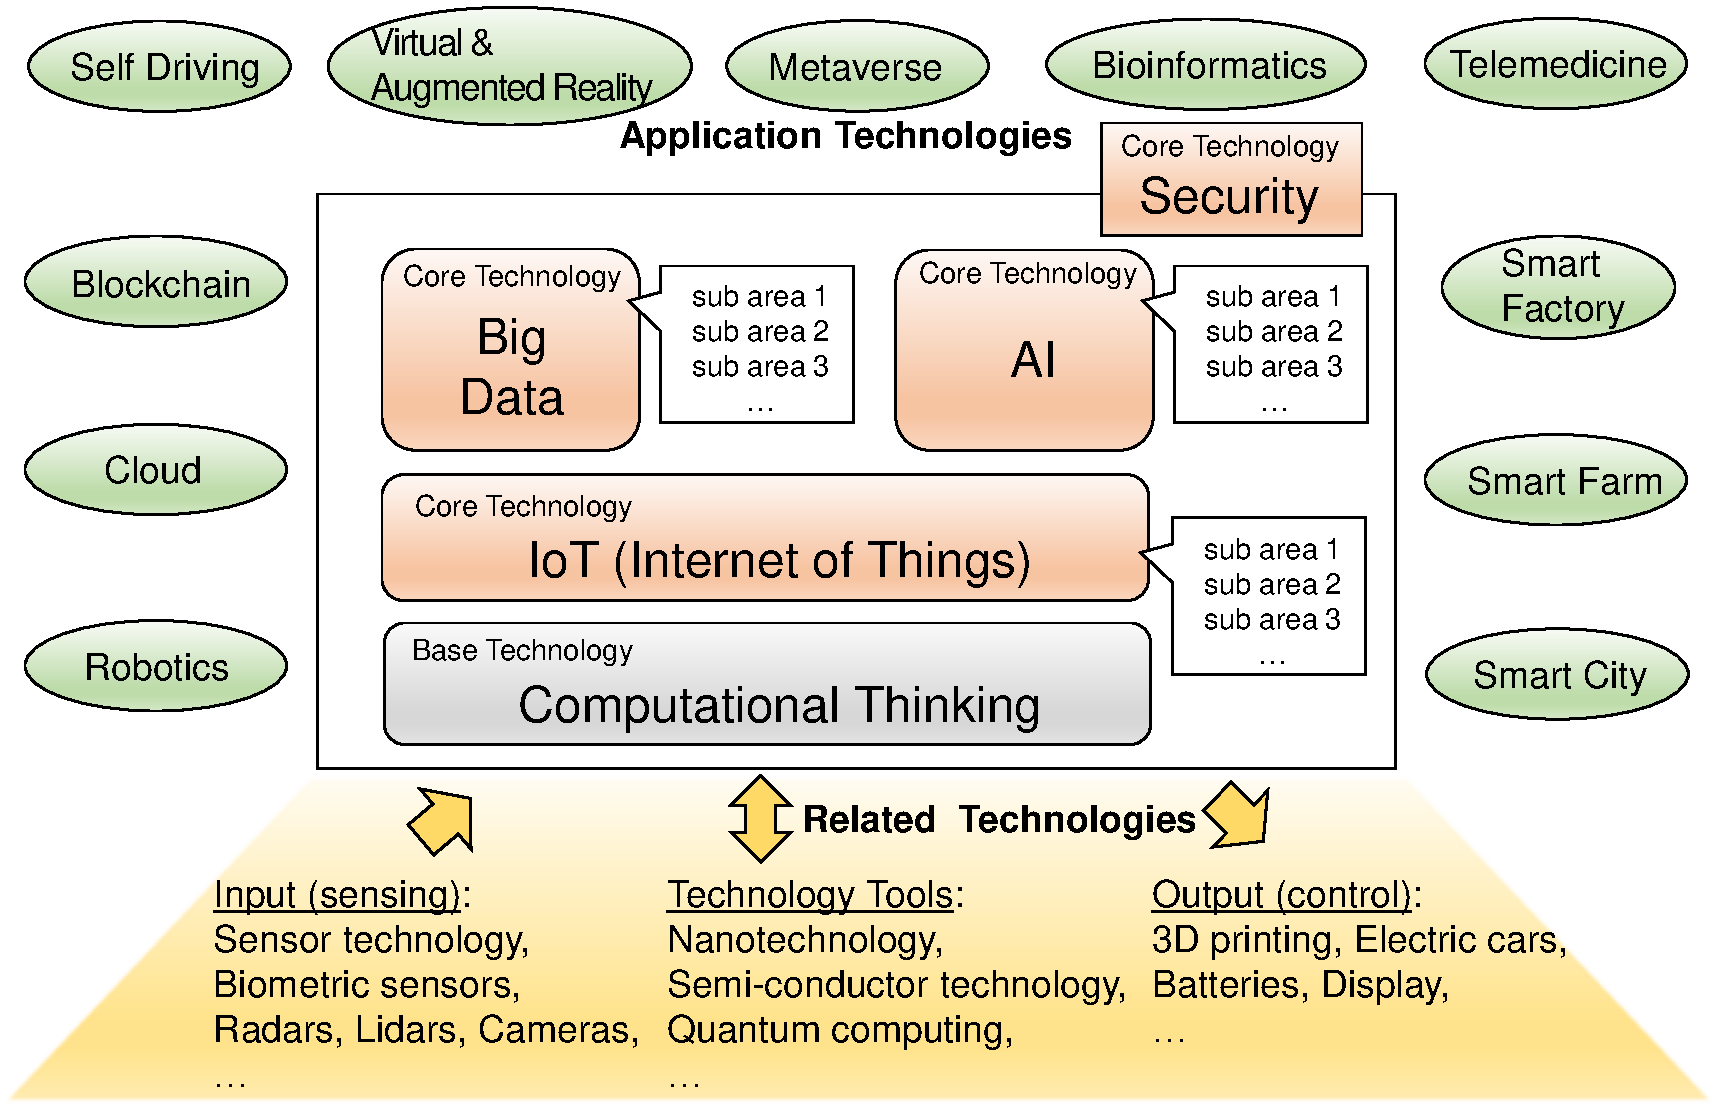
\includegraphics[width=\textwidth]{4IR.pdf}
  \caption{A Bird's eye view of the 4th Industrial Revolution technologies and their relationships.}
  \label{fig:4ir}
\end{figure}

\subsection{Core Technologies}
At the core is a hyper-connected network that can be envisioned as one giant computer. The operations of this computer are sensing, computing, and control/interaction for integrating real and virtual worlds. Big data and AI represent the computing, and the IoT plays the role of the infrastructure. There are also security technologies that protect all these processes. Although not shown here, computer systems form the underlying infrastructure.

\subsection{Base Technologies}
At the base of this paradigm lies computational thinking, which attempts to solve real-life problems computationally. Computational thinking is a fundamental skill required of everyone and not only of computer scientists\,\cite{DBLP:journals/cacm/Wing06}, especially in the 4IR era. Thus, we categorize computational thinking as the base technology, although it may be more appropriate to categorize it as a skill or an approach.

\subsection{Application Technologies}
In Figure 1, example application technologies (by no means exhaustive) based on the core technologies are shown outside the large box and include self driving, VR/AR, metaverse, robotics, smart farms, telemedicine, smart factories, and blockchain. These technologies are already revolutionizing the entire industry. The list is certainly not exhaustive and will keep on growing as AI has become democratized where it is now easy to add intelligence to any existing domain by utilizing open machine learning (ML) platforms such as Google’s TensorFlow and Meta’s PyTorch.

\subsection{Related Technologies}
The related technologies to connect the computer with the real world include various sensor technologies including biometric sensors, radars, lidars, and cameras for the input (sensing part) and 3D printing, electric vehicles, batteries, and display technologies for the output (control/interaction part). Besides, nanotechnology, semi-conductor technology, and quantum computing are widely used for realizing the core technologies as well as the other related technologies. 

In the next sections, we briefly discuss on the core and base technologies and introduce an example application technology on how AI\,(ML) is used in molecular biology, which is a typical approach in bioinformatics. The other application and related technologies are vast, and there are ample opportunities to learn about them through various other media.

% [Add more details on the example application technology in a new section 5]


\section{Base Technology of 4IR}

\subsection{Computational Thinking}
In the 4IR characterized by the metaverse, not only computer scientists, but also general consumers and citizens must be armed with computational thinking. Many countries including the United States, England, and Germany have steadily been revamping their curriculums starting from as early as elementary school (K-12) to strengthen Computer Science education and even require computational thinking\,\cite{10.1145/1929887.1929905,Berry14,DBLP:books/sp/17/DelckerI17,DBLP:books/sp/RH2017}. 
%The International Society for Technology in Education recently defined computational thinking as students “develop[ing] and employ[ing] strategies for understanding and solving problems in ways that lever age the power of technological methods to develop and test solutions” (http://www.iste.org/standards/standards/for-students-2016). 
A pioneering example is the 2014 U.K. educational reform where the subject ``Computing'' was introduced as compulsory in the K-12 curriculum instead of the conventional ICT subject so as to teach students computational thinking, in effect replacing ``how to use'' computers with ``how to be creative'' to understand and change the world\,\cite{Berry14}. 
\emph{Computational thinking} is a methodology ``for understanding and solving problems in ways that leverage the power of technological methods to develop and test solutions''\,\cite{iste2016}.
An alternative description is a set of problem-solving methods that involve formulating problems and solving them in such a way that a computer could also execute\,\cite{wiki-computational-thinking}. 
The four key techniques to computational thinking are decomposition, pattern recognition, abstraction, and algorithms\,\cite{BBC2022}. It involves formulating a problem through summarizing and abstracting a real-world problem and solving it by using an algorithm. During this process, a large problem can be decomposed into smaller problems and solved (divide and conquer). If we borrow the notion ``algorithms + data structures = programs'' by Niklaus Wirth\,\cite{Wirth1976}, computational thinking in short is an approach of solving real life problems by thinking, understanding, analyzing, designing, and executing by computer programs (or computationally).
Since computational thinking constitutes the most basic education to confront 4IR, we categorize it as the base technology.\footnote{Of course some critics worry about ``computational chauvinism''\,\cite{DBLP:journals/cacm/DenningTY17} because computational thinking may not be broad enough to solve all real-life problems.}

\section{Core Technologies of 4IR}

\subsection{AI, Big Data, and Their Integration}

\subsubsection{Integrated Research}
Big data research has been conducted since the 1960’s under the names of file systems, databases, data mining, big data analytics, big data systems, and data science. In the big data era, data has become extremely valuable and is considered to be the oil of the 21st century. Data is also the essential fuel for AI\,(ML). As a result, the collection, storage, processing, and analysis of data has become an indispensable element in any application. AI has been studied since the 1940’s and mimics the human ability to learn, solve problems, and recognize patterns in the form of computer programs. ML is an important branch of AI that uses big data to automatically learn and improve computer algorithms without explicit programming. Platforms such as Google’s TensorFlow have been made public, so the general public can easily use ML in various applications. Applications include self-driving cars, intelligent assistants, AI speakers, AI clerks in marts, automatic defect detection of products in manufacturing, and even professional tasks conducted by doctors and lawyers.
As AI and in particular deep learning heavily rely on large amounts of data, the big data and AI disciplines are becoming increasingly integrated. Within an AI system, ML algorithms account for only a small fraction of all the components in terms of lines of code\,\cite{DBLP:conf/nips/SculleyHGDPECYC15}. In addition to ML code, the significant components include data collection, data verification, feature extraction, and analysis tools. Moreover, according to practitioners of ML, 80--90\% of the efforts in an ML life cycle is spent on data preparation, and many companies have difficulty adopting deep learning due to the need of large amounts of labeled data and the lack of explainability of the trained models\,\cite{DBLP:journals/debu/StonebrakerR19}. In addition, the broad field of data science is not just about ML, but also data mining and database techniques\,\cite{DBLP:journals/debu/Ullman20}. Most recently, even the ML community has started to focus on improving the data for AI performance. Unlike traditional AI where the ML algorithm is of primary interest, the goal is to improve the data while using the same algorithm. This paradigm has been coined as \emph{data-centric AI}\,\cite{data-centric-ai}. In the next sections, we explain two directions of integration: DB to ML and ML to DB.

\subsubsection{DB to ML}
The ML data lifecycle consists of many steps including data understanding, data validation and cleaning, and data preparation\,\cite{DBLP:journals/sigmod/PolyzotisRWZ18}. We summarize how database and data management techniques are being used for these steps.
Better data management can improve ML. For example, data normalization is a common technique to reduce redundancies and anomalies and has been proposed to factorize and improve the speed of ML training as well\,\cite{DBLP:journals/pvldb/ChenKNP17}. Data cleaning has recently been extended and evaluated with the new objective of improving ML accuracy\,\cite{DBLP:conf/icde/LiRBZCZ21}, and data validation techniques are routinely used to check the quality of training data\,\cite{DBLP:conf/kdd/BaylorBCFFHHIJK17}. ML systems are increasingly becoming declarative as well by using schemas and declarative interfaces\,\cite{DBLP:journals/cacm/MolinoR22}. In supervised learning, models are trained using labeled data, and a significant bottleneck is to perform the labeling itself. Data programming\,\cite{DBLP:journals/vldb/RatnerBEFWR20} has been proposed as a way to semi-automatically perform data labeling on unlabeled data where training on large amounts of such data can result in better model accuracy than using smaller amounts of manually-labeled data. 
Another approach is to develop techniques for collecting more datasets that can improve the current training data and lead to better model performance\,\cite{DBLP:journals/tkde/RohHW21}. 
There are new directions in AI that can benefit from data management techniques as well. In particular, \emph{Responsible AI} (also known as \emph{Trustworthy AI}) has become important due to the widespread usage of AI. In addition to simply aim for high accuracy, it is also important to be responsible and guarantee fairness, robustness, privacy, explainability, and transparency among others\,\cite{trustworthy-ai}. \emph{Model fairness} is about removing or coping with bias in the data, which may lead to discriminative predictions\,\cite{compas}. \emph{Robustness} is about ensuring high model accuracy against various noise or poisoning in the data by either removing or fixing them\,\cite{DBLP:conf/icml/SongK019}. \emph{Privacy} is also becoming important as illustrated by a Korean AI chatbot\,\cite{leeluda}, which was famously shut down due to its hate speech and personal information leakage including home addresses. \emph{Explainability} is another important direction where models must be more transparent and understandable when making predictions. Many of these problems can be traced to the training data, so better data management can be a fundamental solution. 

\subsubsection{ML to DB}
The other direction, ML to DB, has been extensively studied recently\,\cite{DBLP:journals/debu/KraskaM0PPRS21}. In this direction, ML techniques are used to improve the performances of various components of a DBMS including indexing, query optimization, and parameter tuning. An index like a B-tree or hash table can be viewed as a function receiving a key attribute value as an input and returning a location of the record with that value. This function can also be learned from data by training a model that is smaller than the index and can be looked up faster\,\cite{DBLP:conf/sigmod/DingMYWDLZCGKLK20}. Query optimization involves searching for the most efficient query plan, and reinforcement learning is a suitable technique as it can help speed up the searching without having to perform exhaustive searching or use handcrafted heuristics, and it only requires a modest amount of training data to approximate the Q-function\,\cite{DBLP:journals/pvldb/MarcusNMZAKPT19}. Parameter tuning in databases can also benefit from reinforcement learning\,\cite{DBLP:journals/pvldb/LiZLG19}. Another line of research is integrating the ML process itself within a database system so that the ML process does not have to be used separately and can take advantage of the database system\,\cite{DBLP:conf/icde/ChaudhuriFB99,DBLP:conf/cidr/BoehmADGIKLPR20}.

\subsubsection{Perspective}
In the future, the integration between big data and AI will only accelerate. Data management is no longer just about data, but needs to be tightly integrated to AI techniques to achieve data-centric AI. At the same time, AI techniques will increasingly complement and possibly even replace database components. While both research directions are very interesting, there must also be considerations of the real needs in the industry as well.

\subsection{Internet of Things (IoT)}
The \emph{IoT} refers to a state where all physical objects are connected over the Internet and can exchange data\,\cite{iot}. People can interact with these things by being connected to the network. Each object obtains information from the surrounding environment through sensors and transmits the information through the network. This concept extends existing Machine to Machine (M2M) communication and is expected to evolve to an Internet of Everything (IoE) where humans, objects, data, and processes all become connected\,\cite{ioe}. Applications for the IoT include smart home, smart farms, smart factories, smart healthcare, and self driving.

\subsubsection{Hyper-Connected Society}
The IoT started as a connection of home appliances and is becoming a foundation for a hyper-connected society. Accordingly, there is a need for more data sensing and fast and reliable networks. Faster communication technology like 5G becomes essential. In December 2018, the three Korean mobile carriers succeeded in transmitting 5G radio waves\,\cite{samsung2019}, thereby ushering in the 5G era where major technologies of 4IR can be supported. As of February 2022, more than 200,000 5G base stations are deployed in South Korea\,\cite{rcrwireless}.

\subsubsection{Definition of 5G and Beyond}
The \emph{5G standard} is developed by the International Telecommunication Union (ITU), which provides the vision and goals, and the 3rd Generation Partnership Project (3GPP) international standardization organization, which develops the technical standards\,\cite{samsung2018}. The key characteristics of 5G are ultra-high speed, ultra-low latency, and hyper-connectivity. Ultra-high speed refers to the high speed of 20Gbps, which is up to 20 times faster than 4G\,\cite{samsung2018}. Ultra-low latency means uninterrupted service where the goal is to reduce latency from tens of milliseconds to around one millisecond\,\cite{samsung2018}. For example, assuming that the time for a self-driving car going at the speed of 100km/h to receive an emergency braking command is 10ms using 4G, the vehicle will move 28cm before stopping. On the other hand, if the delay is 1ms using 5G, the vehicle will only move 2.8cm before starting to stop, which makes the self driving safe. Hyper-connectivity means that the number of devices that can be connected at the same time increases. Table \ref{tab:4G_5G_comparison} shows that the connection density of the IoT and smart devices within 1km$^2$ is 1 million for 5G, which is 10 times larger than that of 4G\,\cite{samsung2018} and brings us a step closer to a wireless smart city. 

\begin{table}[h!]
\begin{center}
\begin{tabular}{ |c|c|c| } 
\hline
Item & 4G & 5G \\\hline\hline
Peak data rate & 1Gbps & 20Gbps \\\hline
User experienced data rate & 10Mbps & 100Mbps \\\hline
Spectrum efficiency & - & X 3 \\\hline
Area traffic capacity & 0.1Mbps/m$^2$ & 10Mbps/m$^2$ \\\hline
Latency & 10ms & 1ms \\\hline
Connection density & 100,000/km$^2$ & 1,000,000/km$^2$ \\\hline
Network energy efficiency & - & X100 \\\hline
Mobility & 350km/h & 500km/h \\
%†Spectrum efficiency: maximum data rate of the communication system within a given bandwidth
%††Area traffic capacity: Maximum transmission capacity within a unit area
\hline
\end{tabular}
\end{center}
\caption{Comparison of 4G and 5G requirements\,\cite{samsung2018}. \emph{Spectrum efficiency} is the maximum data rate of the communication system within a given bandwidth. \emph{Area traffic capacity} is the maximum transmission capacity within a unit area. \emph{Connection density} is the maximum number of devices within a unit area.}
\label{tab:4G_5G_comparison}
\end{table}

More recently the \emph{6G standard} is in development\,\cite{6g}. It is targeting 1 Tbps peak data rate (50 times), 100 microseconds of latency (1 tenth), and 10,000,000/km$^2$ of connection density (10 times), more reliability (100 times) compared with those of 5G (Figure ~\ref{fig:6g}). It is expected 500 billion objects be connected by 2030. There will be more emphasis on heterogeneity to support key 6G services such as truly immersive extended reality (XR), high-fidelity mobile hologram, and digital replica among others, beyond VR/AR and IoT applications\,\cite{samsungwhitepaper}.

\begin{figure}[h!]
  \centering
  \vspace*{-0.4cm}
  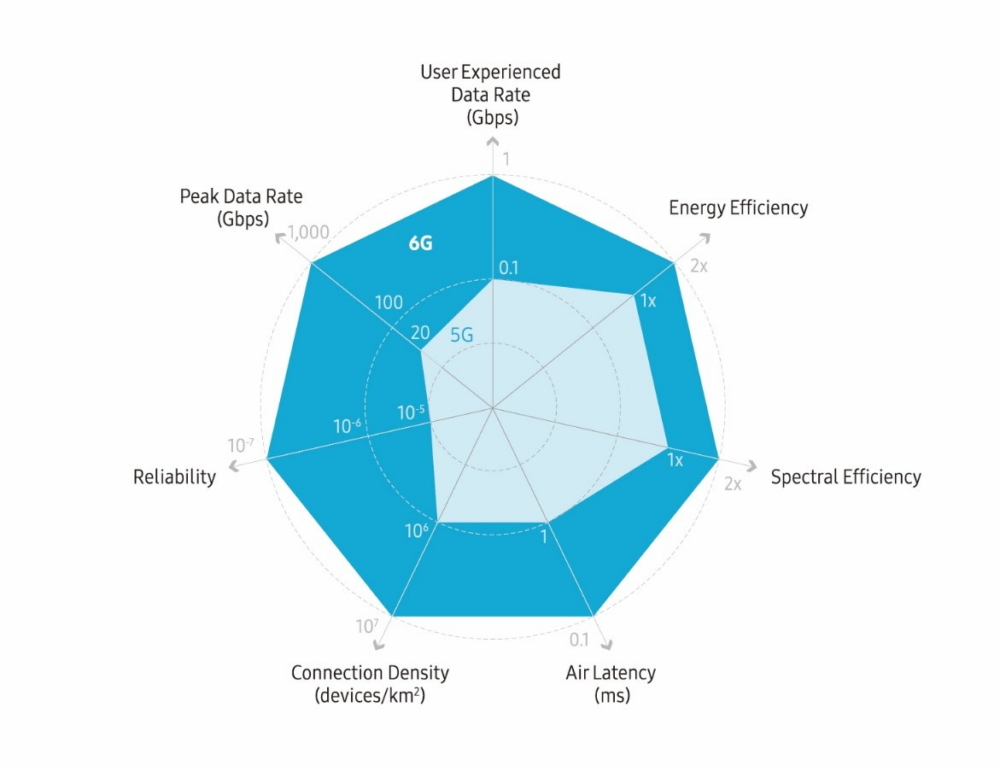
\includegraphics[width=0.71\textwidth]{samsung-6g.jpg}
  \vspace*{-0.5cm}
  \caption{Comparison of 5G and 6G performances. Source: Samsung Electronics\,\cite{samsungwhitepaper}}
  \label{fig:6g}
\end{figure}


\subsection{Security Technology}
%With the advent of innovative new ideas in 4IR, new security issues arise as well. We first need the 5G communication networks and IoT devices to be reliable\,\cite{presidential2019}. For example, in self driving, a temporary disconnect in communication may result in traffic interference, or even life-threatening accidents can occur due to hacking. We also need to prepare for new technologies that break existing security technologies. As the number of IoT devices increases, DDoS (Distributed Denial-of-Service attack) attacks using those devices become easier\,\cite{ddos2016}. In addition, we need to prepare for the vulnerability of asymmetric keys (RSA\,\cite{DBLP:journals/cacm/RivestSA83} and ECC\,\cite{Koblitz1987,DBLP:conf/crypto/Miller85}) against quantum computers\,\cite{presidential2019}. While cyber security is critical in 4IR\,\cite{10.5555/3312394}, we should also make sure it does not stall progress.

%The following quote can be found at the end of the recommendations made by the Korean Presidential Committee on 4IR on October 25th, 2019.
%``As Klaus Schwab revealed in his book ‘The Next’, if cyber security is not guaranteed, all attempts related to 4IR will be like a castle built on sand, which cannot last long. However, security should not become a regulation either. Only when we find a balance between the dilemmas will Korea have a credible status as a hyper-connected nation.’’ Source: Daily Secu (https://www.dailysecu.com) 

A core technology of 4IR, security technology is inextricably related to the other core technologies---big data, AI, and IoT. In this section, we discuss the security issues in each of these three. 

\subsubsection{Security in Big Data}

\begin{itemize}
  \item Data protection and privacy preserving: 
  % As mentioned before, data becomes extremely variable assets as the oil in 4IR era, therefore they are needed to be strictly protected. Privacy preserving also becomes crucial concerns for individuals and societies due to prevalent threat to personal information. 
  Big data poses new threats in data protection and privacy beyond what traditional cryptography and de-identification techniques could counter. For example,
  existing de-identification techniques including $k$-anonymity\,\cite{Sweeney2013} and $l$-diversity\,\cite{Machanavajjhala2006} may be vulnerable to re-identification attacks\,\cite{Henriksen-Bulmer2016}. Thus, differential privacy\,\cite{Cynthia2014} is being considered as an alternative to preserve privacy. \emph{Differential privacy} enables us to publicly share a dataset by conserving statistical properties of groups in the dataset while hiding exact information about individuals in it. Differential privacy has been widely used in collecting and analyzing big data, e.g., by U.S. Census Bureau for showing commuting patterns\,\cite{Ashwin2008}, Google for sharing historical traffic statistics\,\cite{Google2015}, Apple for improving the intelligent personal assistant technology of iOS 10\,\cite{Apple2016}, and Microsoft for implementing telemetry in Windows\,\cite{Bolin2017}. 
  Meanwhile, fast evolution of computing power mainly driven by quantum computing may invalidate existing cryptography systems whose safety is supposed to be guaranteed by extremely high computational complexity\,\cite{bernstein2009introduction}. \emph{Quantum cryptography}\,\cite{Nicolas2002}, in which copying and viewing encrypted message without notification is impossible, can be considered as a countermeasure.
%PPDB deals with obtaining true data mining results without disclosing the basic sensitive data values.

  \item Security in distributed and decentralized information technology\,(IT) infrastructure: In the 4IR era, IT environments become more distributed and decentralized as distributed information processing engines such as Hadoop and Spark are widely used to handle large-scale data, and the IT service platforms move to cloud environments. 
  %To protect such distributed software and hardware infrastructure, traditional countermeasures such as intrusion detection, network security, identity and access management\,(IAM), and distributed denial-of-service\,(DDos) protection have been redesigned. 
  To protect such distributed IT infrastructure, identity and access management\,(IAM), data loss prevention\,(DLP), security information and event management\,(SIEM), business continuity and disaster recovery\,(BCDR) are considered as common countermeasures\,\cite{cloudSecurity} along with traditional cybersecurity techniques such as intrusion detection, network security, and distributed denial-of-service\,(DDoS) protection.
  In addition, a virtualization technique, which securely separates multiple users on a single physical machine, plays a key role to ensure cybersecurity in distributed IT infrastructure, because it is common to share the same resource\,(e.g., machine) with multiple users\,\cite{Darshan2020}. 
%Virtual Machines(VMs) share the underlying hardware and rely on the software level isolation. Several security threats, risks, and vulnerabilities such as malicious VM images, sensitive data leakage, unsecured VM migrations in multi-cloud environments, and backdoor of host OS exist in present virtualization infrastructure that an adversary can utilize to infiltrate the security and privacy of the systems in cloud computing environments. 
Besides, a blockchain is expected to be an important technique to build a decentralized, trustworthy infrastructure even with presence of untrustworthy participants\,\cite{blockchain}. It is being widely used for cryptocurrency and smart contracts.

  \item Security in VR\,/\,AR: % VR/AR can cause serious security issues as it is applied to real life in near future\,\cite{SecurityARVR}. 
  VR\,/\,AR collects a much larger amount of private information about users and their behaviors compared to traditional input devices\,(e.g., keyboards and mouses) and social networking services\,(e.g., Facebook and Twitter)\,\cite{SecurityARVR}. Thus, with smartly forged content, VR\,/\,AR can be powerful means of spreading fake news and social prejudice. At the same time, the guarantee of its availability is crucial when it is utilized in mission-critical tasks such as life rescue, dron control, and production management. We also need to prepare for new security issues such as information sharing between VR\,/\,AR headsets and device protection with physiological or biometric information\,\cite{Guzman2019}.
  % interaction protection such as non-repudiation, authorization, authentication, identifiability, and policy/consent compliance
\end{itemize}


\subsubsection{Security in ML}

ML works with two valuable assets to be protected---data and models, where the former is the input of training and the latter the result. Attack on data is often referred to as \emph{data corruption} or \emph{data poisoning}\,\cite{AIMLThreat}. If the training data is unreliable or biased, ML generates models which may lead to false or unfair decisions. Data corruption or poisoning attacks intentionally manipulate the training data to deceive a model. In principle, such kind of attacks can be prevented with strict access control, confidential data storage, and cryptography. However, the nature of ML training data that a large volume comes from various sources makes this issue more complicated\,\cite{Sarker2020}. In addition, data extraction or exfiltration should be prevented because the training data can be used to infer the behavior of a trained model and can contain proprietary and private information\,\cite{Gary2019}. Attack on a model is often referred to as \emph{model manipulation} or \emph{backdooring} which publishes a model forged for potentially conducting malicious behaviors\,\cite{Gu2017}. The resulting service of such an inflicted model could be problematic. Like data extraction, a model can also be extracted to guess the prediction of the model or to find the hidden parameters influencing the prediction\,\cite{Gary2019}.

%Examples include theft of a proprietary model and enabling attacks on what was designed to be a model. 

\subsubsection{Security in Communications}


In the hyper-connected society realized by 4IR, the cyberattack surface is expanded to all the devices connected to the network---including computers, mobile devices, vehicles, wearable devices, appliances, sensors, and so on\,\cite{forbes2021}. Cyberattacks can target not only the communication between these devices but also the devices themselves. Regarding the IoT communication, lack of IoT security standards is regarded as one of the main obstacles\,\cite{Karie2021}. Because IoT communication is commonly applied to collect and transmit the information in many mission critical scenarios such as self driving, smart factories, and smart healthcare, even a short miscommunication or disconnection by an attack can cause significant damages\,\cite{Moore2020}. 
%For example, when a piece of forged information is delivered to self-driving cars, life-threatening accidents may happen. 
%Regarding the IoT devices, it is possible to trigger false instructions, steal the IoT devices, move the IoT devices to an unauthorized location, comprise the devices on the IoT terminal, and steal or tamper the information
% -->
Pervasive IoT devices also can be exposed to physical threats such as stealing,  unauthorized moving, compromising to steal information or inject forged data, and triggering false instructions that may cause malfunction\,\cite{Xiao2013}. 
%
In addition, traditional DDoS attacks become easier as the number of the devices that can be targeted increases on the IoT platform\,\cite{ddos2016}. 

\begin{comment}
4IR's hyper-connected society connects everything in real time with 5G wireless communication network. Connect everything nature of 5G network considerably expands the cyberattack surface which is all the network connected devices that can be exploited by attackers such as computers, mobile devices, vehicles, wearable devices, appliances, and sensors\,\cite{forbes2021}. Moreover, lack of IoT security standards in 5G network makes the security problems worse. Most of all, 5G networks should be reliable \,\cite{presidential2019}. For example, M2M with 5G network is applied to collect, transmit and manage the information especially in many mission critical scenarios such as Vehicle to Vehicle (V2V), smart grid, smart factory, and SCADA(Supervisory Control And Data Acquisition)\,\cite{Xiao2013}. In self driving with V2V, a temporary disconnect in communication among vehicles due to unreliable 5G network may result in traffic interference, or even life-threatening accidents. Aside from 5G networks, cyber security threats of IoT include false trigger instruction which will active a node incorrectly, stealing the IoT devices, moving the IoT devices to unauthorized location, node compromising attack in the IoT terminal layer, and stealing or tampering the information. We also need to concern the traditional DDoS (Distributed Denial-of-Service attack) attacks become easier as the number of IoT devices that can be participated for the attack increases\,\cite{ddos2016}.
\end{comment}

%5G network is dynamic software-based system which has far more traffic routing points than the current hardware-based, centralized hub-and-spoke designs that 4G has. 
%Many IoT devices are being manufactured with minimal or non-existent cybersecurity measures. These devices are already being used by hackers as entry points to enterprise networks.


\section{Example Application Technology: Molecular Biology}

AI has been actively used in molecular biology, especially for predicting protein structures. Google's DeepMind, well known as the inventor of AlphaGo, created AlphaFold\,\cite{AlphaFold}, the cutting edge AI network for predicting protein structures. Knowing how proteins fold is very useful for scientists to understand the biological processes of every creature. This direction of research can greatly impact on every field of molecular biology, from helping overcome disease and quickly discovering new medicines to revealing the mysteries of life.

% subset of machine learning in which multilayered neural networks learn from vast amounts of data.

Consistent with the trend of 4IR, \emph{deep learning}, a subset of ML in which deep\,(i.e., multilayered) neural networks learn from vast amounts of data, is attracting more and more attention in molecular biology as well. Notably, deep learning relieves the need for rigorous feature engineering done by domain experts, because a deep neural network itself can accept high-dimensional input as well as decide the importance of each feature and derive latent features\,\cite{Jisna2021}. Directly using raw input data without help from domain experts not only automates and speeds up the entire process but also increases the scalability of the input data. This benefit stands out especially in the 4IR era, because deep learning can digest unprecedented amounts of big data generated by DNA sequencing. 
For example, DeepTFactor\,\cite{DeepTFactor} is designed to predict a \emph{transcription factor\,(TF)}, which is a protein that specifically binds to DNA and regulates gene transcription. Identifying TFs is regarded as the starting point of the inspection of transcriptional regulatory systems\,\cite{DeepTFactor}. As shown in Figure \ref{fig:DeepTFactor}, DeepTFactor, which consists of convolutional neural networks (CNNs),  receives a protein sequence and predicts whether the given protein sequence is a TF. Three CNNs with different filter sizes can learn diverse latent features, and their outputs are concatenated to exploit all of these latent features; then, another CNN learns the mapping between the latent features and the class label\,(i.e., TF or non-TF). As a result, DeepTFactor achieves higher accuracy than previous TF classification tools\,\cite{DeepTFactor}. Overall, deep learning has become a powerful tool for various studies in molecular biology\,\cite{Webb2018}.

\begin{figure}[h]
  \centering
  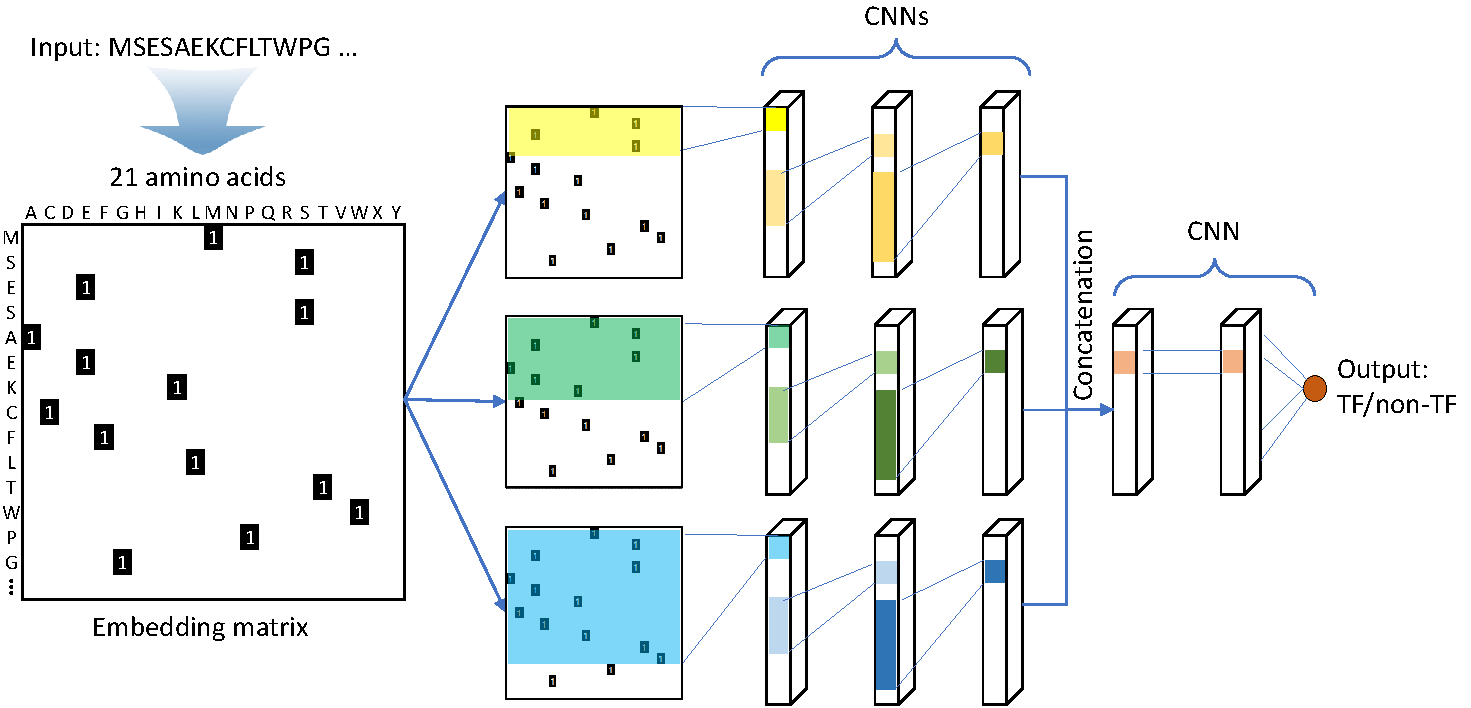
\includegraphics[width=0.9\textwidth]{DeepTFactor.pdf}
  \caption{Deep neural network architecture of DeepTFactor. A shade color indicates the connection between the input and output of a convolution operation. Source: Kim et al.\,\cite{DeepTFactor}}
  \label{fig:DeepTFactor}
\end{figure}


\section{Conclusion}
In summary, we categorized the various technologies in 4IR and covered important core technologies---big data, AI, IoT, and security. In addition, we presented an application of AI in molecular biology. We hope this article will serve as a useful stepping stone for a comprehensive understanding of the technologies related to 4IR.

\section*{Acknowledgment}
The authors deeply appreciate the invaluable help from Steven E. Whang in completing Section 4.1.

\bibliographystyle{plain}
\small
\itemsep=1pt
%\bibliography{references}

\begin{thebibliography}{10}

\bibitem{6g}
6{G} (network).
\newblock \url{https://en.wikipedia.org/wiki/6G_(network)}.
\newblock Accessed June 12th, 2022.

\bibitem{Apple2016}
Apple previews {iOS} 10, the biggest {iOS} release ever.
\newblock
  \url{https://www.apple.com/newsroom/2016/06/apple-previews-ios-10-biggest-ios-release-ever/}.
\newblock Accessed June 15th, 2022.

\bibitem{blockchain}
Blockchain in {W}ikipedia.
\newblock \url{https://en.wikipedia.org/wiki/Blockchain}.
\newblock Accessed June 15th, 2022.

\bibitem{iste2016}
Computational thinking.
\newblock \url{http://www.iste.org/standards/standards/for-students-2016}.
\newblock Accessed June 10th, 2022.

\bibitem{wiki-computational-thinking}
Computational thinking.
\newblock \url{https://en.wikipedia.org/wiki/Computational_thinking}.
\newblock Accessed June 10th, 2022.

\bibitem{data-centric-ai}
Data-centric {AI}.
\newblock \url{https://datacentricai.org/}.
\newblock Accessed June 5th, 2022.

\bibitem{ddos2016}
Ddos attack that disrupted internet was largest of its kind in history, experts
  say.
\newblock
  \url{https://www.theguardian.com/technology/2016/oct/26/ddos-attack-dyn-mirai-botnet}.
\newblock Accessed June 10th, 2022.

\bibitem{compas}
How we analyzed the compas recidivism algorithm.
\newblock
  \url{https://www.propublica.org/article/how-we-analyzed-the-compas-recidivism-algorithm}.
\newblock Accessed June 5th, 2022.

\bibitem{Hyundai2022}
Hyundai motor company's mid-to-long term electrification strategy disclosed (in
  {K}orean).
\newblock \url{https://www.hyundai.co.kr/news/CONT0000000000012239}.
\newblock Accessed August 1st, 2022.

\bibitem{ioe}
Internet of everything.
\newblock
  \url{https://www.techtarget.com/iotagenda/definition/Internet-of-Everything-IoE}.
\newblock Accessed June 10th, 2022.

\bibitem{iot}
Internet of things.
\newblock \url{https://www.oracle.com/internet-of-things/what-is-iot/}.
\newblock Accessed June 10th, 2022.

\bibitem{BBC2022}
Introduction to computational thinking.
\newblock \url{https://www.bbc.co.uk/bitesize/guides/zp92mp3/revision/1}.
\newblock Accessed June 5th, 2022.

\bibitem{Reuters2022}
The long road to electric cars.
\newblock \url{https://graphics.reuters.com/AUTOS-ELECTRIC/USA/mopanyqxwva/}.
\newblock Accessed August 1st, 2022.

\bibitem{Schwab2016b}
Schwab {K}laus. {T}he fourth industrial revolution: what it means, how to
  respond.
\newblock
  \url{https://www.weforum.org/agenda/2016/01/the-fourth-industrial-revolution-what-it-means-and-how-to-respond/}.
\newblock World Economic Forum, June 2016.

\bibitem{SecurityARVR}
The security risks of {AR} and {VR}.
\newblock \url{ https://defpr.com/the-security-risks-of-ar-and-vr/}.
\newblock Accessed June 15th, 2022.

\bibitem{leeluda}
A {S}outh {K}orean chatbot shows just how sloppy tech companies can be with
  user data.
\newblock
  \url{https://slate.com/technology/2021/04/scatterlab-lee-luda-chatbot-kakaotalk-ai-privacy.html}.
\newblock Accessed June 5th, 2022.

\bibitem{Google2015}
Tackling urban mobility with technology.
\newblock
  \url{https://europe.googleblog.com/2015/11/tackling-urban-mobility-with-technology.html}.
\newblock Accessed June 15th, 2022.

\bibitem{AIMLThreat}
Top 5 security threats facing artificial intelligence and machine learning.
\newblock
  \url{https://hubsecurity.com/blog/cyber-security/security-threats-for-ai-and-machine-learning/}.
\newblock Accessed June 15th, 2022.

\bibitem{trustworthy-ai}
Trustworthy {AI}.
\newblock \url{https://www.ibm.com/watson/trustworthy-ai}.
\newblock Accessed June 5th, 2022.

\bibitem{cloudSecurity}
What is cloud security?
\newblock \url{https://www.ibm.com/topics/cloud-security}.
\newblock Accessed July 25th, 2022.

\bibitem{forbes2021}
Why {5G} networks are disrupting the cybersecurity industry.
\newblock
  \url{https://www.forbes.com/sites/forbestechcouncil/2021/10/29/why-5g-networks-are-disrupting-the-cybersecurity-industry/?sh=4b997d5a1fe9}.
\newblock Accessed June 15th, 2022.

\bibitem{10.1145/1929887.1929905}
Valerie Barr and Chris Stephenson.
\newblock Bringing computational thinking to {K}-12: What is involved and what
  is the role of the computer science education community?
\newblock {\em ACM Inroads}, 2(1):48--54, February 2011.

\bibitem{DBLP:conf/kdd/BaylorBCFFHHIJK17}
Denis Baylor, Eric Breck, Heng{-}Tze Cheng, Noah Fiedel, Chuan~Yu Foo, Zakaria
  Haque, Salem Haykal, Mustafa Ispir, Vihan Jain, Levent Koc, Chiu~Yuen Koo,
  Lukasz Lew, Clemens Mewald, Akshay~Naresh Modi, Neoklis Polyzotis, Sukriti
  Ramesh, Sudip Roy, Steven~Euijong Whang, Martin Wicke, Jarek Wilkiewicz, Xin
  Zhang, and Martin Zinkevich.
\newblock {TFX:} {A} tensorflow-based production-scale machine learning
  platform.
\newblock In {\em KDD}, pages 1387--1395. {ACM}, 2017.

\bibitem{bernstein2009introduction}
Daniel~J Bernstein.
\newblock Introduction to post-quantum cryptography.
\newblock In {\em Post-quantum cryptography}, pages 1--14. Springer, 2009.

\bibitem{Berry14}
Miles Berry.
\newblock This is for everyone {K}12 computer science in {E}ngland.
\newblock In {\em The 21st KAST International Symposium (KAST 20th Anniversary
  International Symposium), Plaza Hotel, Seoul}, 2014.

\bibitem{DBLP:conf/cidr/BoehmADGIKLPR20}
Matthias Boehm, Iulian Antonov, Sebastian Baunsgaard, Mark Dokter, Robert
  Ginth{\"{o}}r, Kevin Innerebner, Florijan Klezin, Stefanie~N. Lindstaedt,
  Arnab Phani, Benjamin Rath, Berthold Reinwald, Shafaq Siddiqui, and
  Sebastian~Benjamin Wrede.
\newblock Systemds: {A} declarative machine learning system for the end-to-end
  data science lifecycle.
\newblock In {\em CIDR}, 2020.

\bibitem{DBLP:conf/icde/ChaudhuriFB99}
Surajit Chaudhuri, Usama~M. Fayyad, and Jeff Bernhardt.
\newblock Scalable classification over {SQL} databases.
\newblock In {\em ICDE}, pages 470--479. {IEEE}, 1999.

\bibitem{DBLP:journals/pvldb/ChenKNP17}
Lingjiao Chen, Arun Kumar, Jeffrey~F. Naughton, and Jignesh~M. Patel.
\newblock Towards linear algebra over normalized data.
\newblock {\em Proc. {VLDB} Endow.}, 10(11):1214--1225, 2017.

\bibitem{Guzman2019}
Jaybie~A. de~Guzman, Kanchana Thilakarathna, and Aruna Seneviratne.
\newblock Security and privacy approaches in mixed reality: {A} literature
  survey.
\newblock {\em {ACM} Comput. Surv.}, 52(6):110:1--110:37, 2020.

\bibitem{DBLP:books/sp/17/DelckerI17}
Jan Delcker and Dirk Ifenthaler.
\newblock Computational thinking as an interdisciplinary approach to computer
  science school curricula: {A} {G}erman perspective.
\newblock In Peter~J. Rich and Charles~B. Hodges, editors, {\em Emerging
  Research, Practice, and Policy on Computational Thinking}, pages 49--62.
  Springer, 2017.

\bibitem{DBLP:journals/cacm/DenningTY17}
Peter~J. Denning, Matti Tedre, and Pat Yongpradit.
\newblock Misconceptions about computer science.
\newblock {\em Commun. {ACM}}, 60(3):31--33, 2017.

\bibitem{Bolin2017}
Bolin Ding, Janardhan Kulkarni, and Sergey Yekhanin.
\newblock Collecting telemetry data privately.
\newblock In {\em NeurIPS}, pages 3571--3580, 2017.

\bibitem{DBLP:conf/sigmod/DingMYWDLZCGKLK20}
Jialin Ding, Umar~Farooq Minhas, Jia Yu, Chi Wang, Jaeyoung Do, Yinan Li,
  Hantian Zhang, Badrish Chandramouli, Johannes Gehrke, Donald Kossmann,
  David~B. Lomet, and Tim Kraska.
\newblock {ALEX:} an updatable adaptive learned index.
\newblock In {\em SIGMOD}, pages 969--984. {ACM}, 2020.

\bibitem{Cynthia2014}
Cynthia Dwork and Aaron Roth.
\newblock The algorithmic foundations of differential privacy.
\newblock {\em Found. Trends Theor. Comput. Sci.}, 9(3-4):211--407, 2014.

\bibitem{Nicolas2002}
Nicolas Gisin, Gr\'egoire Ribordy, Wolfgang Tittel, and Hugo Zbinden.
\newblock Quantum cryptography.
\newblock {\em Rev. Mod. Phys.}, 74:145--195, March 2002.

\bibitem{Gu2017}
Tianyu Gu, Brendan Dolan{-}Gavitt, and Siddharth Garg.
\newblock Badnets: Identifying vulnerabilities in the machine learning model
  supply chain.
\newblock {\em CoRR}, abs/1708.06733, 2017.

\bibitem{Henriksen-Bulmer2016}
Jane Henriksen{-}Bulmer and Sheridan Jeary.
\newblock Re-identification attacks--{A} systematic literature review.
\newblock {\em Int. J. Inf. Manag.}, 36(6):1184--1192, 2016.

\bibitem{Jisna2021}
V.A. Jisna and P.B. Jayaraj.
\newblock Protein structure prediction: Conventional and deep learning
  perspectives.
\newblock {\em Protein Journal}, 40:522--544, 2021.

\bibitem{AlphaFold}
John Jumper et~al.
\newblock Highly accurate protein structure prediction with {AlphaFold}.
\newblock {\em Nature}, 596:583--589, 2021.

\bibitem{Karie2021}
Nickson~M. Karie, Nor~Masri Sahri, Wencheng Yang, Craig Valli, and Victor~R.
  Kebande.
\newblock A review of security standards and frameworks for {I}o{T}-based smart
  environments.
\newblock {\em {IEEE} Access}, 9:121975--121995, 2021.

\bibitem{DeepTFactor}
Gi~Bae Kim, Ye~Gao, Bernhard~O. Palsson, and Sang~Yup Lee.
\newblock {DeepTFactor}: A deep learning-based tool for the prediction of
  transcription factors.
\newblock {\em Proceedings of the National Academy of Sciences of the United
  States of America (PNAS)}, 118(2):e2021171118, 2021.

\bibitem{DBLP:journals/debu/KraskaM0PPRS21}
Tim Kraska, Umar~Farooq Minhas, Thomas Neumann, Olga Papaemmanouil, Jignesh~M.
  Patel, Christopher R{\'{e}}, and Michael Stonebraker.
\newblock {ML}-in-databases: Assessment and prognosis.
\newblock {\em {IEEE} Data Eng. Bull.}, 44(1):3--10, 2021.

\bibitem{lasi2014industry}
Heiner Lasi, Peter Fettke, Hans-Georg Kemper, Thomas Feld, and Michael
  Hoffmann.
\newblock Industry 4.0.
\newblock {\em Business \& information systems engineering}, 6(4):239--242,
  2014.

\bibitem{DBLP:journals/pvldb/LiZLG19}
Guoliang Li, Xuanhe Zhou, Shifu Li, and Bo~Gao.
\newblock Qtune: {A} query-aware database tuning system with deep reinforcement
  learning.
\newblock {\em Proc. {VLDB} Endow.}, 12(12):2118--2130, 2019.

\bibitem{DBLP:conf/icde/LiRBZCZ21}
Peng Li, Xi~Rao, Jennifer Blase, Yue Zhang, Xu~Chu, and Ce~Zhang.
\newblock Clean{ML}: {A} study for evaluating the impact of data cleaning on
  {ML} classification tasks.
\newblock In {\em ICDE}, pages 13--24. {IEEE}, 2021.

\bibitem{Machanavajjhala2006}
Ashwin Machanavajjhala, Johannes Gehrke, Daniel Kifer, and Muthuramakrishnan
  Venkitasubramaniam.
\newblock l-diversity: privacy beyond k-anonymity.
\newblock In {\em ICDE}, pages 24--35. IEEE, 2006.

\bibitem{Ashwin2008}
Ashwin Machanavajjhala, Daniel Kifer, John~M. Abowd, Johannes Gehrke, and Lars
  Vilhuber.
\newblock Privacy: Theory meets practice on the map.
\newblock In {\em ICDE}, pages 277--286. IEEE, 2008.

\bibitem{DBLP:journals/pvldb/MarcusNMZAKPT19}
Ryan~C. Marcus, Parimarjan Negi, Hongzi Mao, Chi Zhang, Mohammad Alizadeh, Tim
  Kraska, Olga Papaemmanouil, and Nesime Tatbul.
\newblock Neo: {A} learned query optimizer.
\newblock {\em Proc. {VLDB} Endow.}, 12(11):1705--1718, 2019.

\bibitem{Gary2019}
Gary McGraw, Richie Bonett, Harold Figueroa, and Victor Shepardson.
\newblock Security engineering for machine learning.
\newblock {\em Computer}, 52(8):54--57, 2019.

\bibitem{DBLP:journals/cacm/MolinoR22}
Piero Molino and Christopher R{\'{e}}.
\newblock Declarative machine learning systems.
\newblock {\em Commun. {ACM}}, 65(1):42--49, 2022.

\bibitem{Moore2020}
Samuel~J. Moore, Chris~D. Nugent, Shuai Zhang, and Ian Cleland.
\newblock Io{T} reliability: a review leading to 5 key research directions.
\newblock {\em {CCF} Trans. Pervasive Comput. Interact.}, 2(3):147--163, 2020.

\bibitem{Xiao2013}
Xiao Nie and Xiaobing Zhai.
\newblock {M2M} security threat and security mechanism research.
\newblock In {\em ICCSNT}, pages 906--909, 2013.

\bibitem{DBLP:journals/sigmod/PolyzotisRWZ18}
Neoklis Polyzotis, Sudip Roy, Steven~Euijong Whang, and Martin Zinkevich.
\newblock Data lifecycle challenges in production machine learning: {A} survey.
\newblock {\em {SIGMOD} Rec.}, 47(2):17--28, 2018.

\bibitem{DBLP:journals/vldb/RatnerBEFWR20}
Alexander Ratner, Stephen~H. Bach, Henry~R. Ehrenberg, Jason~A. Fries, Sen Wu,
  and Christopher R{\'{e}}.
\newblock Snorkel: rapid training data creation with weak supervision.
\newblock {\em {VLDB} J.}, 29(2-3):709--730, 2020.

\bibitem{DBLP:books/sp/RH2017}
Peter~J. Rich and Charles~B. Hodges, editors.
\newblock {\em Emerging Research, Practice, and Policy on Computational
  Thinking}.
\newblock Springer, 2017.

\bibitem{Rifkin2011}
Jeremy Rifkin.
\newblock {\em The Third Industrial Revolution}.
\newblock Palgrave MacMillan, 2011.

\bibitem{DBLP:journals/tkde/RohHW21}
Yuji Roh, Geon Heo, and Steven~Euijong Whang.
\newblock A survey on data collection for machine learning: {A} {B}ig data -
  {AI} integration perspective.
\newblock {\em {IEEE} Trans. Knowl. Data Eng.}, 33(4):1328--1347, 2021.

\bibitem{samsung2019}
Samsung.
\newblock {5G} launches in {K}orea.
\newblock
  \url{https://images.samsung.com/is/content/samsung/p5/global/business/networks/insights/white-paper/5g-launches-in-korea-get-a-taste-of-the-future/5G-Launches-in-Korea-Get-a-taste-of-the-future.pdf}.
\newblock 2019.

\bibitem{samsung2018}
Samsung.
\newblock Who \& {H}ow: making {5G} {NR} standards.
\newblock
  \url{https://images.samsung.com/is/content/samsung/p5/global/business/networks/insights/white-paper/who-and-how_making-5g-nr-standards/who-and-how_making-5g-nr-standards.pdf}.
\newblock 2018.

\bibitem{samsungwhitepaper}
Samsung.
\newblock 6{G} the next hyper-connected experience for all.
\newblock White paper, Samsung Research, 2020.

\bibitem{Sarker2020}
Iqbal~H. Sarker, A.~S.~M. Kayes, Shahriar Badsha, Hamed AlQahtani, Paul~A.
  Watters, and Alex Ng.
\newblock Cybersecurity data science: an overview from machine learning
  perspective.
\newblock {\em J. Big Data}, 7(1):1--29, 2020.

\bibitem{Schwab2016}
Klaus Schwab.
\newblock {\em The Fourth Industrial Revolution}.
\newblock Portfolio Penguin, 2016.

\bibitem{DBLP:conf/nips/SculleyHGDPECYC15}
D.~Sculley, Gary Holt, Daniel Golovin, Eugene Davydov, Todd Phillips, Dietmar
  Ebner, Vinay Chaudhary, Michael Young, Jean{-}Fran{\c{c}}ois Crespo, and Dan
  Dennison.
\newblock Hidden technical debt in machine learning systems.
\newblock In {\em NeurIPS}, pages 2503--2511, 2015.

\bibitem{DBLP:conf/icml/SongK019}
Hwanjun Song, Minseok Kim, and Jae{-}Gil Lee.
\newblock {SELFIE:} refurbishing unclean samples for robust deep learning.
\newblock In {\em ICML}, pages 5907--5915. {PMLR}, 2019.

\bibitem{DBLP:journals/debu/StonebrakerR19}
Michael Stonebraker and El~Kindi Rezig.
\newblock Machine learning and {B}ig data: What is important?
\newblock {\em {IEEE} Data Eng. Bull.}, 42(4):3--7, 2019.

\bibitem{Sweeney2013}
Latanya Sweeney.
\newblock k-anonymity: A model for protecting privacy.
\newblock {\em Int. J. Uncertain. Fuzziness Knowl. Based Syst.},
  10(5):557--570, 2002.

\bibitem{Darshan2020}
Darshan Tank, Akshai Aggarwal, and Nirbhay Chaubey.
\newblock {\em Cyber Security Aspects of Virtualization in Cloud Computing
  Environments: Analyzing Virtualization-Specific Cyber Security Risks}, pages
  283--299.
\newblock January 2020.

\bibitem{rcrwireless}
Juan~Pedro Tomas.
\newblock South korea ends {F}ebruary with almost 203,000 5g base stations:
  Report.
\newblock
  \url{https://rcrwireless.com/20220331/5g/south-korea-ends-february-almost-203000-5g-base-stations-report},
  March 2022.

\bibitem{DBLP:journals/debu/Ullman20}
Jeffrey~D. Ullman.
\newblock The battle for data science.
\newblock {\em {IEEE} Data Eng. Bull.}, 43(2):8--14, 2020.

\bibitem{Webb2018}
Sarah Webb.
\newblock Deep learning for biology.
\newblock {\em Nature}, 554:555--557, 2018.

\bibitem{DBLP:journals/cacm/Wing06}
Jeannette~M. Wing.
\newblock Computational thinking.
\newblock {\em Commun. {ACM}}, 49(3):33--35, 2006.

\bibitem{Wirth1976}
Niklaus Wirth.
\newblock {\em Algorithms + Data Structures = Programs}.
\newblock Prentice-Hall, 1976.

\end{thebibliography}


\end{document}

\end{opinion}
\end{opinionsection}

% put the name of your special issue below
\begin{articlesection}{Widening the Impact of Data Engineering through Innovations in Education, Interfaces, and Features}

\begin{article}
{Automated Grading of SQL Queries}
{Bikash Chandra and S.\ Sudarshan}
\documentclass[11pt]{article}
%\documentclass[11pt,dvipdfm]{article}

\usepackage{deauthor}
\usepackage{url}            % simple URL typesetting
\usepackage{graphicx}
\usepackage{times}
\usepackage{fancyvrb}
\usepackage{comment}

% \graphicspath{{authorname/}}

\begin{document}

%\title{MLflow: An Open Platform for Machine Learning Experimentation, Reproducibility and Production}
%\title{MLflow: An Open Platform for the End-to-End Machine Learning Lifecycle}
\title{Accelerating the Machine Learning Lifecycle with {MLflow}}

% The \author macro works with any number of authors. There are two
% commands used to separate the names and addresses of multiple
% authors: \And and \AND.
%
% Using \And between authors leaves it to LaTeX to determine where to
% break the lines. Using \AND forces a line break at that point. So,
% if LaTeX puts 3 of 4 authors names on the first line, and the last
% on the second line, try using \AND instead of \And before the third
% author name.

\author{
  \textbf{Matei Zaharia, Andrew Chen, Aaron Davidson, Ali Ghodsi, Sue Ann Hong, Andy Konwinski,}\\
  \textbf{Siddharth Murching, Tomas Nykodym, Paul Ogilvie, Mani Parkhe, Fen Xie, Corey Zumar} \\
  Databricks Inc.\\
  %% examples of more authors
  %% \And
  %% Coauthor \\
  %% Affiliation \\
  %% Address \\
  %% \texttt{email} \\
  %% \AND
  %% Coauthor \\
  %% Affiliation \\
  %% Address \\
  %% \texttt{email} \\
  %% \And
  %% Coauthor \\
  %% Affiliation \\
  %% Address \\
  %% \texttt{email} \\
  %% \And
  %% Coauthor \\
  %% Affiliation \\
  %% Address \\
  %% \texttt{email} \\
}

\maketitle

\begin{abstract}
Machine learning development creates multiple new challenges that are not present in a traditional software development lifecycle.
These include keeping track of the myriad inputs to an ML application (e.g., data versions, code and tuning parameters), reproducing results, and production deployment.
In this paper, we summarize these challenges from our experience with Databricks customers, and describe MLflow, an open source platform we recently launched to streamline the machine learning lifecycle.
MLflow covers three key challenges: experimentation, reproducibility, and model deployment, using generic APIs that work with any ML library, algorithm and programming language.
The project has a rapidly growing open source community, with over 50 contributors since its launch in June 2018.
\end{abstract}

\section{Introduction}

Machine learning development requires solving new problems that are not part of the standard software development lifecycle.
For example, while traditional software has a well-defined set of product features to be built, ML development tends to revolve around \emph{experimentation}: the ML developer will constantly experiment with new datasets, models, software libraries, tuning parameters, etc.~to optimize a business metric such as model accuracy.
Because model performance depends heavily on the input data and training process, \emph{reproducibility} is paramount throughout ML development.
Finally, in order to have business impact, ML applications need to be \emph{deployed} to production, which means both deploying a model in a way that can be used for inference (e.g., REST serving) and deploying scheduled jobs to regularly update the model.
This is especially challenging when deployment requires collaboration with another team, such as application engineers who are not ML experts.

Based on our conversations with dozens of Databricks customers that use machine learning, these lifecycle problems are a major bottleneck in practice.
Although today's ML libraries provide tools for part of the lifecycle, there are no standard systems and interfaces to manage the full process.
For example, TensorFlow offers a training API and a Serving system~\cite{tfx}, but TensorFlow Serving cannot easily be used for models from another ML library, or from an incompatible version of TensorFlow.
In practice, an organization will need to run models from multiple ML libraries, TensorFlow versions, etc., and has to design its own infrastructure for this task.


Faced with these challenges, many organizations try to ``lock down'' the ML development process to obtain reproducibility and deployability.
Some organizations develop internal guidelines for ML development, such as which libraries one can use that the production team will support.
Others develop internal \emph{ML platforms} (e.g., Facebook's FBLearner~\cite{fblearner}, Uber's Michelangelo~\cite{michelangelo} and Google's TFX~\cite{tfx}): APIs that ML developers must use in order to build deployable models.
Unfortunately, both approaches limit ML developers in the algorithms and libraries they can use, decreasing their ability to experiment, and both create substantial engineering work whenever the ML developers want to use new libraries or models.

%Some organizations ask each ML team to manage its own infrastructure, which is expensive.
%Others try to develop shared \emph{ML platforms} that data scientists must use to build their models (e.g., Facebook's FBLearner~\cite{fblearner} and Uber's Michelangelo~\cite{michelangelo}), but this approach also has challenges, because model developers are limited to the algorithms and libraries supported by the platform and cannot easily experiment with others.

In this paper, we summarize our experience with ML lifecycle challenges at Databricks customers and describe MLflow, an open source ML platform we are developing to address these challenges.
MLflow's key principle is an \emph{open interface} design, where data scientists and engineers can bring their own training code, metrics, and inference logic while benefitting from a structured development process.
%MLflow leverages simple, generic interfaces such as Docker containers and REST APIs to achieve this goal.
For example, a ``model'' saved in MLflow can simply be a Python function (and associated library dependencies) that MLflow then knows how to deploy in various environments (e.g., batch or real-time scoring).
Other MLflow abstractions are likewise based on generic interfaces, such as REST APIs and Docker containers.
Compared to existing ML platforms like FBLearner, Michelangelo and TFX, this open interface design gives users flexibility and control while retaining the benefits of lifecycle management.
%Moreover, MLflow's open source nature enables easily sharing ML work across organizations.
The current version of MLflow provides APIs for experiment tracking, reproducible runs and model packaging and deployment, usable in Python, Java and R.
We describe these APIs and some sample MLflow use cases to show how the system can streamline the machine learning lifecycle.

\section{Challenges in Machine Learning Development}

ML faces many of the challenges in traditional software development, such as testing, code review, monitoring, etc.
In other ways, however, ML applications are different from traditional software, and present new problems.

One of the main differences is that the goal in machine learning is to \emph{optimize} a specific metric, such as prediction accuracy, instead of simply meeting a set of functional requirements.
For example, for a retailer, every 1\% improvement in prediction accuracy for a recommendation engine might lead to millions of dollars in revenue, so the ML team working on this engine will continuously want to improve the model.
This means that ML developers wish to continuously experiment with the latest models, software libraries, etc.,~to improve target metrics.
Beyond this difference in objective, ML applications are more complex to manage because their performance depends on training data, tuning, and concerns such as overfitting that do not occur in other applications.
%This means that reproducibility of these runtime conditions is important.
Finally, ML applications are often developed by teams or individuals with very different expertise, and hand-off between these individuals can be challenging.
For example, a data scientist might be an expert at ML training, and use her skills to create a model, but she might need to pass the model to a software engineer for deployment within an application.
Any errors in this process (e.g., mismatched software versions or data formats) might lead to incorrect results that are hard for a software engineer without ML knowledge to debug.

Based on these requirements in working with ML, we found four challenges to arise repeatedly at ML users:

\vspace{-0.6em}
\paragraph{1. Multitude of tools.} Hundreds of software tools cover each phase of ML development, from data preparation to model training to deployment. However, unlike traditional software development, where teams select \emph{one} tool for each phase, ML developers usually want to try \emph{every} available tool (e.g., algorithm) to see whether it improves results. For example, a team might try multiple preprocessing libraries (e.g., Pandas and Apache Spark) to featurize data; multiple model types (e.g. trees and deep learning); and even multiple frameworks for the same model type (e.g., TensorFlow and PyTorch) to run various models published online by researchers. %This diversity of tools means that ML teams need to use and productionize dozens of libraries.

\vspace{-0.6em}
\paragraph{2. Experiment tracking.} Machine learning results are affected by dozens of configurable parameters, ranging from the input data to hyperparameters and preprocessing code. Whether an individual is working alone or on a team, it is difficult to track which parameters, code, and data went into each experiment to produce a model.

\vspace{-0.6em}
\paragraph{3. Reproducibility.} Without detailed tracking, teams often have trouble getting the same code to work again. For example, a data scientist passing her training code to an engineer for use in production might see problems if the engineer modifies it, and even a user working alone needs to reliably reproduce old results to stay productive. %Even ML researchers frequently experience this problem when trying to reproduce published work.

\vspace{-0.6em}
\paragraph{4. Production deployment.} Moving an application to production can be challenging, both for inference and training. First, there are a plethora of possible inference environments, such as REST serving, batch scoring and mobile applications, but there is no standard way to move models from any library to these diverse environments. Second, the model training pipeline also needs to be reliably converted to a scheduled job, which requires care to reproduce the software environments, parameters, etc.~used in development.
Production deployment is especially challenging because it often requires passing the ML application to a different team with less ML expertise.

~

\vspace{-0.6em}
To address these problems, we believe that ML development processes should be explicitly designed to promote reproducibility, deployability, etc. The challenge is how to do so while leaving maximum flexibility for ML developers to build the best possible model. This led us to the open interface design philosophy for MLflow.

\section{MLflow Overview}

To structure the ML development process while leaving users maximum flexibility, we built MLflow around an \emph{open interface} philosophy: the system should define general interfaces for each abstraction (e.g., a training step, a deployment tool or a model) that allow users to bring their own code or workflows.
For example, many existing ML tools represent models using a serialization format, such as TensorFlow graphs~\cite{abadi2016tensorflow}, ONNX~\cite{onnx} or PMML~\cite{pmml}, when passing them from training to serving. This restricts applications to using specific libraries.
In contrast, in MLflow, a model can be represented simply as a Python function (and library dependency information), so any development tool that knows how to run a Python function can run such a model.
For more specialized deployment tools, a model can also expose other interfaces called ``flavors" (e.g., an ONNX graph) while still remaining viewable as just a Python function.
As another example, MLflow exposes most of its features through REST APIs that can called from any programming language.

More specifically, MLflow provides three components, which can either be used together or separately:

\begin{itemize}
\item \textbf{MLflow Tracking}, which is an API for recording experiment runs, including code used, parameters, input data, metrics, and arbitrary output files. These runs can then be queried through an API or UI.

\item\textbf{MLflow Projects}, a simple format for packaging code into reusable projects. Each project defines its environment (e.g., software libraries required), the code to run, and parameters that can be used to call the project programmatically in a multi-step workflow or in automated tools such as hyperparameter tuners.

\item\textbf{MLflow Models}, a generic format for packaging models (both the code and data required) that can work with diverse deployment tools (e.g., batch and real-time inference). %The goal is to give users of the model (e.g., a production engineer) a consistent interface for working with models built in different tools.
\end{itemize}

%We next sketch these components in turn; full documentation on them is available at \url{mlflow.org}.

\subsection{MLflow Tracking}

MLflow Tracking is an API for logging and querying \emph{experiment runs}, which consist of parameters, code versions, metrics and arbitrary output files called \emph{artifacts}. Users can start/end runs and log metrics, parameters and artifacts using simple API calls, as shown below using MLflow's Python API:

\begin{Verbatim}[frame=single,fontsize=\small,samepage=true]
# Log parameters, which are arbitrary key-value pairs
mlflow.log_param("num_dimensions", 8)
mlflow.log_param("regularization", 0.1)

# Log metrics; each metric can also be updated throughout the run
mlflow.log_metric("accuracy", 0.8)
mlflow.log_metric("r2", 0.4)

# Log artifacts (arbitrary output files)
mlflow.log_artifact("precision_recall.png")
\end{Verbatim}

MLflow Tracking API calls can be inserted anywhere users run code (e.g., standalone applications or Jupyter notebooks running in the cloud). The tracking API logs results to a local directory by default, but it can also be configured to log over the network to a server, allowing teams to share a centralized MLflow tracking server and compare results from multiple developers.

Once users have recorded runs, MLflow allows users to query them through an API or web-based UI (Figure~\ref{fig:tracking-ui}). This UI includes the ability to organize runs into groups called Experiments, search and sort them, and compare groups of runs, enabling users to build a custom leaderboard for each of their ML problems and even compare results across teams. The UI is inspired by experiment visualization tools such as Sacred~\cite{sacred}, ModelDB~\cite{modeldb} and TensorBoard~\cite{tensorboard}, and supports similar visualizations and queries.

\begin{figure}[h]
\centering
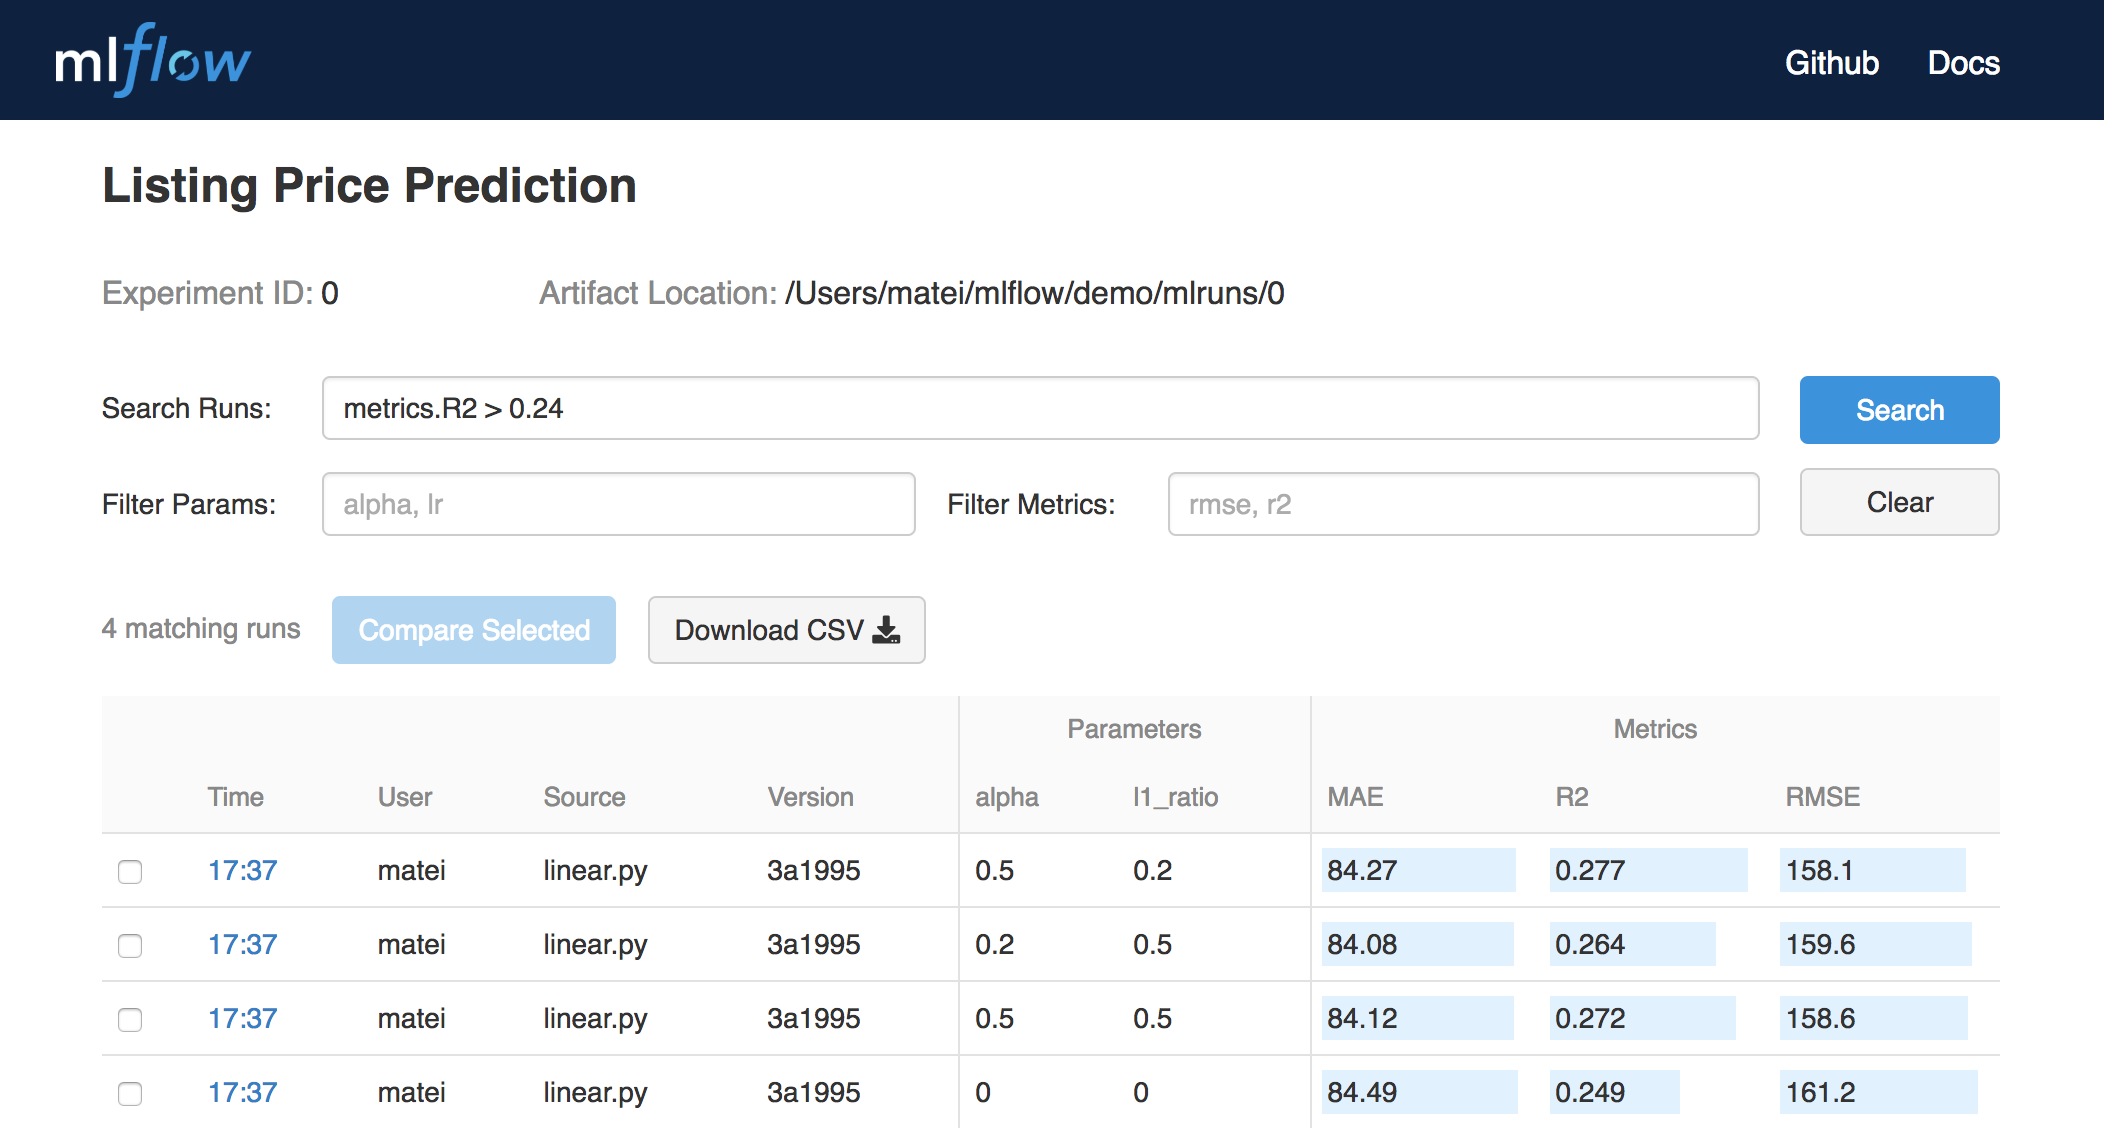
\includegraphics[bb=0 0 1052 564,width=\textwidth]{tracking.png}
\caption{MLflow Tracking UI showing several runs in an experiment. Clicking each run lists its metrics, artifacts and output details and lets the user post comments about the run.}
\label{fig:tracking-ui}
\end{figure}

\subsection{MLflow Projects}

MLflow Projects provide a simple format for packaging reproducible data science code. Each project is simply a directory with code or a Git repository, and uses a descriptor file to specify its dependencies and how to run the code. A MLflow Project is defined by a simple YAML file called MLproject, as shown below:

\begin{Verbatim}[frame=single,fontsize=\small,samepage=true]
name: My Project
conda_env: conda.yaml
entry_points:
  main:
    parameters:
      data_file: path
      alpha: {type: float, default: 0.1}
    command: "python train.py --reg-param {alpha} --data {data_file}"
\end{Verbatim}


Projects can specify their dependencies through a Conda environment or (in an upcoming release) a Docker container specification. A project may also have multiple entry points for invoking runs, with named parameters that downstream users can provide without understanding the internals of the project.

Users can run projects using the \texttt{mlflow run} command line tool, either from local files or a Git repository:

\begin{Verbatim}[frame=single,fontsize=\small,samepage=true]
mlflow run git@github.com:databricks/mlflow-example.git -P alpha=0.5
\end{Verbatim}

Alternatively, projects can be called programmatically using MLflow's API. This can be used to implement multi-step workflows or to pass projects a ``black box'' into automated tools such as hyperparameter search~\cite{hyperopt}.

In either case, MLflow will automatically set up the project's runtime environment and execute it. If the code inside the project uses the MLflow Tracking API, MLflow will also remember the project version executed (that is, the Git commit) and show an \texttt{mlflow run} command to re-execute it in its UI. Finally, MLflow projects can also be submitted to cloud platforms such as Databricks for remote execution.

\subsection{MLflow Models}

MLflow Models are a convention for packaging machine learning models in multiple formats called ``flavors'', allowing diverse tools to understand the model at different levels of abstractions. MLflow also offers a variety of built-in tools to deploy models in its standard favors. For example, the same model can be deployed as a Docker container for REST serving, as an Apache Spark user-defined function (UDF) for batch inference, or into cloud-managed serving platforms like Amazon SageMaker and Azure ML.

Each MLflow Model is simply stored as a directory containing arbitrary files and an MLmodel YAML file that lists the flavors it can be used in and additional metadata about how it was created:

\begin{Verbatim}[frame=single,fontsize=\small,samepage=true]
time_created: 2018-02-21T13:21:34.12
run_id: c4b65fc2c57f4b6d80c6e58a9dcb9f01
flavors:
  sklearn:
    sklearn_version: 0.19.1
    pickled_model: model.pkl
  python_function:
    loader_module: mlflow.sklearn
    pickled_model: model.pkl
\end{Verbatim}

In this example, the model can be used with tools that support either the \texttt{sklearn} or \texttt{python\_function} model flavors. For example, the MLflow SciKit-Learn library knows how to load a \texttt{sklearn} model as a SciKit-Learn Python object, but other deployment tools, such as running the model in a Docker HTTP server, only understand lower-level flavors like \texttt{python\_function}.
In addition, models logged using MLflow Tracking APIs will automatically include a reference to that run's unique ID, letting users discover how they were built.

\section{Example Use Cases}

In this section, we describe three sample MLflow use cases to highlight how users can leverage each component.

\vspace{-0.6em}
\paragraph{Experiment tracking.} A European energy company is using MLflow to track and update hundreds of energy grid models. This team's goal is to build a time series model for every major energy producer (e.g., power plant) and consumer (e.g., factory), monitor these using standard metrics, and combine the predictions to drive business processes such as pricing. Because a single team is responsible for hundreds of models, possibly using different ML libraries, it was important to have a standard development and tracking process. The team has standardized on using Jupyter notebooks for development, MLflow Tracking for metrics, and Databricks jobs for inference.

\vspace{-0.6em}
\paragraph{Reproducible projects.} An online marketplace is using MLflow Projects to package deep learning jobs using Keras and run them in the cloud. Each data scientist develops models locally on his or her laptop using a small dataset, checks them into a Git repository with an MLproject file, and submits remote runs of the project to GPU instances in the cloud for large-scale training or hyperparameter search. Using MLflow Projects makes it easy to create the same software environment in the cloud and share project code between different data scientists.

\vspace{-0.6em}
\paragraph{Model packaging.} The data science team at an e-commerce site is using MLflow Models to package recommendation models for use by application engineers. The technical challenge here was that the recommendation application includes both a standard, ``off-the-shelf'' recommendation model and custom business logic for pre- and post-processing. For example, the application might include custom code to make sure that the recommended items are diverse. This business logic needs to change in sync with the model, and the data science team wants to control both the business logic and the model, without having to submit a patch to the web application each time this logic has to change.
Moreover, the team wants to A/B test distinct models with distinct versions of the processing logic.
The solution was to package both the recommendation model and the custom logic using the \texttt{python\_function} flavor in an MLflow Model, which can then be deployed and tested as a single unit. %This allows production engineers to deploy the recommendation code as they please without the processing logic falling out of sync with the model.

\section{Related Work}

Many software systems aim to simplify ML development.
The closest to our work are the end-to-end ``ML platforms'' at large web companies.
For example, Facebook's FBLearner lets users write reusable workflow steps that run over data in Apache Hive~\cite{fblearner};
Uber's Michelangelo gives users a toolkit of algorithms to choose from that it can automatically train and deploy~\cite{michelangelo}; and Google's TFX provides data preparation and serving tools around TensorFlow~\cite{tfx}.
Anecdotally, these platforms greatly accelerate ML development, showing the benefits of standardizing the ML lifecycle.
However, they generally restrict users to a specific set of algorithms or libraries, so teams are on their own when they step outside these boundaries.
Our goal in MLflow is to let users easily bring their own tools and software in as many steps in the process as possible through our ``open interface'' design.
This includes custom training steps, inference code, and logged parameters and artifacts.

Other systems also tackle specific problems within the ML lifecycle. For example, Sacred~\cite{sacred}, ModelDB~\cite{modeldb} and TensorBoard~\cite{tensorboard} let users track experiments; PMML~\cite{pmml} and ONNX~\cite{onnx} are cross-library model serialization formats; Clipper~\cite{clipper} can deploy arbitrary models as Docker containers; and CDE~\cite{cde}, CodaLab~\cite{codalab}, Binder~\cite{binder} and Repo2Docker~\cite{repo2docker} enable reproducible software runs. MLflow combines these concepts with new ones, such as multi-flavor model packaging, into a unified system design and API.

\section{Conclusion}

For machine learning to have widespread commercial impact, organizations require the same kinds of reliable engineering processes around ML that exist in other engineering disciplines such as software development. In this paper, we have described some of the key challenges that differentiate ML development from traditional software development, such as experimentation, reproducibility, and reliable production deployment. We have also described MLflow, a software platform that can structure the machine learning lifecycle while giving users broad flexibility to use their own ML algorithms, software libraries and development processes.
MLflow is available as open source software at \url{https://www.mlflow.org}.


{\small

\begin{thebibliography}{10}

  \bibitem{abadi2016tensorflow}
  M.~Abadi, P.~Barham, J.~Chen, Z.~Chen, A.~Davis, J.~Dean, M.~Devin,
    S.~Ghemawat, G.~Irving, M.~Isard, et~al.
  \newblock {TensorFlow: A System for Large-Scale Machine Learning}.
  \newblock In {\em OSDI}, volume~16, pages 265--283, 2016.

  \bibitem{tfx}
  D.~Baylor, E.~Breck, H.-T. Cheng, N.~Fiedel, C.~Y. Foo, Z.~Haque, S.~Haykal,
    M.~Ispir, V.~Jain, L.~Koc, C.~Y. Koo, L.~Lew, C.~Mewald, A.~N. Modi,
    N.~Polyzotis, S.~Ramesh, S.~Roy, S.~E. Whang, M.~Wicke, J.~Wilkiewicz,
    X.~Zhang, and M.~Zinkevich.
  \newblock Tfx: A tensorflow-based production-scale machine learning platform.
  \newblock In {\em Proceedings of the 23rd ACM SIGKDD International Conference
    on Knowledge Discovery and Data Mining}, KDD '17, pages 1387--1395, New York,
    NY, USA, 2017. ACM.

  \bibitem{hyperopt}
  J.~Bergstra, B.~Komer, C.~Eliasmith, D.~Yamins, and D.~D. Cox.
  \newblock Hyperopt: a python library for model selection and hyperparameter
    optimization.
  \newblock {\em Computational Science and Discovery}, 8(1):014008, 2015.

  \bibitem{binder}
  {Binder}.
  \newblock \url{https://mybinder.org}, 2018.

  \bibitem{clipper}
  D.~Crankshaw, X.~Wang, G.~Zhou, M.~J. Franklin, J.~E. Gonzalez, and I.~Stoica.
  \newblock Clipper: A low-latency online prediction serving system.
  \newblock In {\em Proceedings of the 14th USENIX Conference on Networked
    Systems Design and Implementation}, NSDI'17, pages 613--627, Berkeley, CA,
    USA, 2017. USENIX Association.

  \bibitem{fblearner}
  J.~Dunn.
  \newblock Introducing {FBLearner Flow}: Facebook’s {AI} backbone.
  \newblock
    \url{https://code.fb.com/core-data/introducing-fblearner-flow-facebook-s-ai-backbone/}.

  \bibitem{repo2docker}
  J.~Forde, T.~Head, C.~Holdgraf, Y.~Panda, G.~Nalvarte, M.~Pacer, F.~Perez,
    B.~Ragan-Kelley, and E.~Sundell.
  \newblock Reproducible research environments with repo2docker.
  \newblock ICML, 07/2018 2018.

  \bibitem{tensorboard}
  Google.
  \newblock Tensorboard: Visualizing learning.
  \newblock \url{https://www.tensorflow.org/guide/summaries_and_tensorboard}.

  \bibitem{pmml}
  A.~Guazzelli, W.-C. Lin, and T.~Jena.
  \newblock {\em PMML in Action: Unleashing the Power of Open Standards for Data
    Mining and Predictive Analytics}.
  \newblock CreateSpace, Paramount, CA, 2nd edition, 2012.

  \bibitem{cde}
  P.~J. Guo.
  \newblock {CDE}: A tool for creating portable experimental software packages.
  \newblock {\em Computing in Science and Engineering}, 14(4):32--35, 2012.

  \bibitem{michelangelo}
  J.~Hermann and M.~D. Balso.
  \newblock Meet {Michelangelo}: Uber’s machine learning platform.
  \newblock \url{https://eng.uber.com/michelangelo/}.

  \bibitem{sacred}
  {K}laus {G}reff, {A}aron {K}lein, {M}artin {C}hovanec, {F}rank {H}utter, and
    {J}\"urgen {S}chmidhuber.
  \newblock {T}he {S}acred {I}nfrastructure for {C}omputational {R}esearch.
  \newblock In {K}aty {H}uff, {D}avid {L}ippa, {D}illon {N}iederhut, and
    M.~{P}acer, editors, {\em {P}roceedings of the 16th {P}ython in {S}cience
    {C}onference}, pages 49 -- 56, 2017.

  \bibitem{codalab}
  P.~Liang et~al.
  \newblock {CodaLab}.
  \newblock \url{https://worksheets.codalab.org}, 2018.

  \bibitem{onnx}
  {ONNX Group}.
  \newblock {ONNX}.
  \newblock \url{https://onnx.ai}.

  \bibitem{modeldb}
  M.~Vartak, H.~Subramanyam, W.-E. Lee, S.~Viswanathan, S.~Husnoo, S.~Madden, and
    M.~Zaharia.
  \newblock Modeldb: A system for machine learning model management.
  \newblock In {\em Proceedings of the Workshop on Human-In-the-Loop Data
    Analytics}, HILDA '16, pages 14:1--14:3, New York, NY, USA, 2016. ACM.

  \end{thebibliography}


}
%\bibliographystyle{abbrv}
%\bibliography{paper}

\end{document}

\end{article}

\begin{article}
{Towards Technology-Enabled Learning of Relational Query Processing}
{Sourav S.\ Bhowmick and Hui Li}
\documentclass[11pt]{article}
\usepackage{deauthor,times,graphicx}
\usepackage{subfig}
\graphicspath{{submissions/teach-qp-bhowmick/figs/}}

\usepackage{balance}
\usepackage{xspace}
\usepackage{url}
\usepackage{hyperref}
\usepackage{authblk}
\usepackage{cite}

\newcommand{\ie}{\emph{i.e.,}\xspace}
\newcommand{\eg}{\emph{e.g.,}\xspace}
\newcommand{\etc}{\emph{etc.}\xspace}
\newcommand{\wrt}{\emph{w.r.t.}\xspace}
\newcommand{\resp}{\emph{resp.,}\xspace}
\newcommand{\etal}{\emph{et al.}\xspace}
\newcommand{\btitle}[1]{\vspace{1ex}\noindent \textbf{#1}}
\newcommand{\eat}[1]{}
\def\EndOfProof{\nolinebreak\ \hfill\rule{1.5mm}{2.7mm}}

\begin{document}
\title{Towards Technology-Enabled Learning of Relational Query Processing}
\author{Sourav S.\ Bhowmick$\,^{\star}$~~~and~~~Hui Li$\,^{\diamond}$\\ $^{\star}$~Nanyang Technological University (NTU), Singapore, \texttt{assourav@ntu.edu.sg}\\
$^{\diamond}$~Xidian University, China, \texttt{hli@xidian.edu.cn}
}
\maketitle

\begin{abstract}
The database systems course has gained increasing prominence in academic institutions due to the convergence of widespread usage of relational database management system (\textsc{rdbms}) in the commercial world, the growth of Data Science, and the increasing importance of lifelong learning. A key learning goal of learners taking such a course is to learn how \textsc{sql} queries are processed in an \textsc{rdbms} in \emph{practice}. Most database courses supplement traditional modes of teaching with technologies such as off-the-shelf \textsc{rdbms} to provide hands-on opportunities to learn database concepts used in practice. Unfortunately, these systems are not designed for effective and efficient pedagogical support for the topic of relational query processing. In this vision paper, we identify novel problems and challenges that need to be addressed in order to provide effective and efficient technological supports for learning this topic. We also identify opportunities for \textit{data-driven} education brought by any effective solutions to these problems. Lastly, we briefly report the \textsc{truss} system that we are currently building to address these challenges.
\end{abstract}


%====================================================================================================
\section{Introduction}  %17
\label{sec1}
%====================================================================================================
Learning is the acquisition of knowledge or skills through study, experience, or being taught~\cite{Gross}.  It is not just listening and accepting what we are taught, but understanding and experiencing them. Education, on the other hand, is the acquisition of knowledge through a process of receiving or giving systematic instruction. Hence, although learning and education are closely related, the former has a broader scope and impact. Specifically, learning can be facilitated through education, personal development, schooling, training or experience. It is not limited to a certain age or period in life. Indeed, while formal education for young adult learners at universities has been the focus of educational provisions in the industrial age, the digital age is now seeing an increased experimentation of  ``lifelong learning''~\cite{unesco} with provisions such as  work-study programmes for early career and mid-career individuals, and digital learning initiatives.

The growing demand for lifelong learning coupled with the widespread use of relational database management system (\textsc{rdbms}) in the commercial world and the growth of Data Science as a discipline have generated increasing demand of database-related courses in academic institutions. Learners from diverse fields and experiences aspire to take these courses, even with limited Computer Science backgrounds~\cite{panel}. In a computer science degree program, the key goal of a database systems course is to teach learners how to \emph{build} a database system. On the other hand, the focus of the course in a data science program is to be able to \emph{control} a database system effectively. To facilitate both these goals, it is paramount for learners to learn  how \textsc{sql} queries are processed in an \textsc{rdbms} in practice. Traditionally, this learning goal is achieved through textbooks and lectures. Specifically, major database textbooks~\cite{dbtext,cow} introduce \textit{general} (\ie not tied to any specific \textsc{rdbms}) theories and principles associated with relational query processing and optimization using natural language-based narratives and visual examples. This allows a learner to gain a general understanding of \textsc{sql} query execution strategies. 

It is well-established in education that \textit{effective} use of technology has a positive impact on learning~\cite{HXK12}. It causes learners to be more motivated and engaged, thus, enabling them to retain more information. It also increases hands-on learning opportunities. In fact, technology is best used as \textit{``a supplement to normal teaching rather than as a replacement for it''}~\cite{HXK12}. Hence, in order to promote effective and efficient learning for diverse individuals in full recognition of the complexity of the topic of relational query processing,  \emph{learner-friendly} tools are paramount to  augment the traditional modes of learning (\ie textbook, lecture).  Indeed, database systems courses in major institutions around the world supplement traditional style of learning with the usage of off-the-shelf \textsc{rdbms}. Unfortunately, these \textsc{rdbms} are not designed for pedagogical support. Although they enable hands-on learning opportunities to build database applications and pose a wide variety of \textsc{sql} queries over it, very limited effective and efficient learner-friendly support, beyond the visualization of \textit{query execution plans}, is provided for understanding and experiencing the processing and optimization of these queries \textit{in practice} by the underlying relational query engine. 


Given the challenges faced by learners to learn \textsc{sql}~\cite{MAF21}, there has been increasing research efforts to build tools and techniques to facilitate comprehension of complex \textsc{sql} statements~\cite{KV+12,HM+22,MRY19,MF21,LZ+20,DG11}, automated grading of \textsc{sql} queries~\cite{BC+15}, and so on. However, scant attention has been paid to explore technologies that can enable learning of relational query processing~\cite{lantern,neuron,picasso}. In this paper, we articulate a vision shaped by the following fundamental questions: (a) What are the key problems that we need to address to facilitate technology-enabled learning of relational query processing in practice? (b) How can the potential solutions to these problems support data-driven education with the goal of making teaching and learning practices more effective and efficient?  Specifically, our vision calls for a \textit{learning-centric}, \textit{generic}, and \textit{psychology-aware} approach grounded on the \textit{theories} of motivation and learning to address these challenges. Note that by no means we claim that the list of problems discussed in this article is exhaustive. The pervasive desire here is to galvanize the data management community to explore this nascent inter-disciplinary topic at the intersection of learning sciences and data management by leveraging these problems as the seed.

The rest of the paper is organized as follows. In Section~\ref{back}, we briefly introduce relevant \textit{motivation theories} that are at the foundation of learning and may potentially impact the design of any learner-centric, technology-enabled solutions for learning. Section~\ref{sec:challenge} introduces the  key novel research challenges that need to be addressed in order to realize the vision. We briefly report the \textsc{truss} system which we are currently building to address these challenges in Section~\ref{sec:truss}. The last section concludes this paper.
  
%====================================================================================================
\section{Motivation Theories}
\label{back} 
%====================================================================================================

Learning is impacted by \textit{motivation}, which is the process that initiates, guides, and maintains goal-oriented behavior~\cite{kazdin}. Specifically, motivation impacts how likely a learner is willing to learn. Since effective use of technology in learning has positive impact on motivation,  we need to understand motivation theories and their impact on learning. These theories should underpin any effective technological solutions for facilitating learning. In this section, we first briefly describe key theories related to motivation proposed in the domain of education psychology. Next, we highlight how these theories can guide technology-enabled solutions for learning. In the next section, we shall identify novel research issues that are grounded on these theories to facilitate learning of relational query processing.

\vspace{1ex} \noindent \textbf{Motivation theories.} Motivation can be broadly characterised into two types,\textit{ intrinsic} and \textit{extrinsic}~\cite{RD00}.\textit{ Intrinsic motivation} is the act of doing an activity purely for the joy of doing it whereas \textit{extrinsic motivation} is to do something due to the influence of external  rewards or punishments (\eg good grades, jobs). Although the latter is not optimal for learning, research suggests that extrinsic motivation is prevalent~\cite{RD00,DV+91} and may pave the way to intrinsic motivation. That is, a learner may initiate learning due to external factors but the motivation may morph to an intrinsic one during task engagement. 
 
Regardless of the type of motivation, \textit{Achievement Goal Theory}~\cite{AP12} argues that all motivation are essentially linked to one's goals that can take two forms, namely \textit{performance goals} and \textit{mastery goals}. The former is caused by satisfaction of one's ego (\eg appearing superior to one's peers) whereas the latter is aligned with intrinsic motivation and is grounded on the pure desire to master a skill or concept. The \textit{Expectancy Value Theory}~\cite{WE00} postulates that expectation and value of learning a skill or concept have direct impact on the performance and task choice of a learner. To elaborate further,  an individual's effort and performance for a task are influenced by their expectation of success or failure.  Note that expectations and values themselves are influenced by how a learner assess their competency and perceived task difficulty.  If a learner has felt satisfaction in undertaking a similar task in the past, then it is more likely they will put effort to the current task.  However, if past experience shows the task is either too difficult to be completed or not sufficiently difficult enough then they may not engage with it. The \textit{Flow Theory}~\cite{NL09} describes a  psychological state in which an individual is purely intrinsically motivated to learn without any external factors. Such state is said to occur when the task is neither too difficult to cause helplessness or frustration nor too easy to make a learner bored. 

\vspace{1ex} \noindent\textbf{Motivation theories in technology-enabled learning frameworks.} Every learner has intrinsic or extrinsic motivation to reach their learning goals. Hence, any technology-enabled learning framework should be cognizant of the above theories in order to cultivate motivation to learn. Specifically, technologies to supplement learning of relational query processing and optimization should support the followings:

\begin{itemize} \itemsep = -0.5ex

\item Learners may learn relational query processing due to intrinsic or extrinsic motivation. It is important that any technological framework support both and facilitate transformation of extrinsic motivation to intrinsic one during the course of interacting with it. 

\item  Increase learners' satisfaction of successful completion of the task of learning relational query processing as well as facilitate flow state of learners to move to the Goldilock's zone (\ie learning relational query processing concepts is neither too difficult nor too easy). 

\end{itemize}

%====================================================================================================
\section{Research Issues}
\label{sec:challenge}
%====================================================================================================
In this section, we outline novel \textit{learner-centric} research issues in the burgeoning topic of technology-enabled learning of relational query processing.  It is worth noting that although technology engages and motivates learners, it is advantageous for learning only when it is aligned to with what is to be learned~\cite{HXK12}. Hence, the issues we focus for technological support are learning about query execution plans, exploration of \textit{alternative query plans} in a plan space, and cost estimation of a physical query plan. Observe that all these issues are typically covered by a database systems course.  A common theme that cuts across these issues is the pervasive desire for motivation theory-aware tools and techniques that aim to \emph{supplement} existing off-the-shelf \textsc{rdbms} to facilitate learning of these issues. We begin with a brief background on relational query plans that learners typically encounter in a database systems course. 

%====================================================================================================
\subsection{Query Plans}
%====================================================================================================

Given an arbitrary \textsc{sql} query, an \textsc{rdbms} generates a \textit{query execution plan} (\textsc{qep}) to execute it.  A \textsc{qep}  consists of a collection of physical operators organized in form of a tree, namely the \textit{physical operator tree} (\textit{operator tree} for brevity). Figure~\ref{fig:alter_plans}(a) depicts an example \textsc{qep} with a collection of physical operators. Each physical operator, \eg \texttt{SEQUENTIAL SCAN}, \texttt{INDEX SCAN}, takes as input one or more data streams and produces an output one. A \textsc{qep} explicitly describes how the underlying \textsc{rdbms} shall execute the given query. Notably, given an \textsc{sql} query, there are many different query plans, other than the \textsc{qep}, for executing it.  We refer to these different plans (other than the \textsc{qep}) as \textit{alternative query plans} (\textsc{aqp}).  Figures~\ref{fig:alter_plans}(b)-(c) depict two examples of \textsc{aqp}. 
 
 
 \begin{figure}[t]
	\centering
	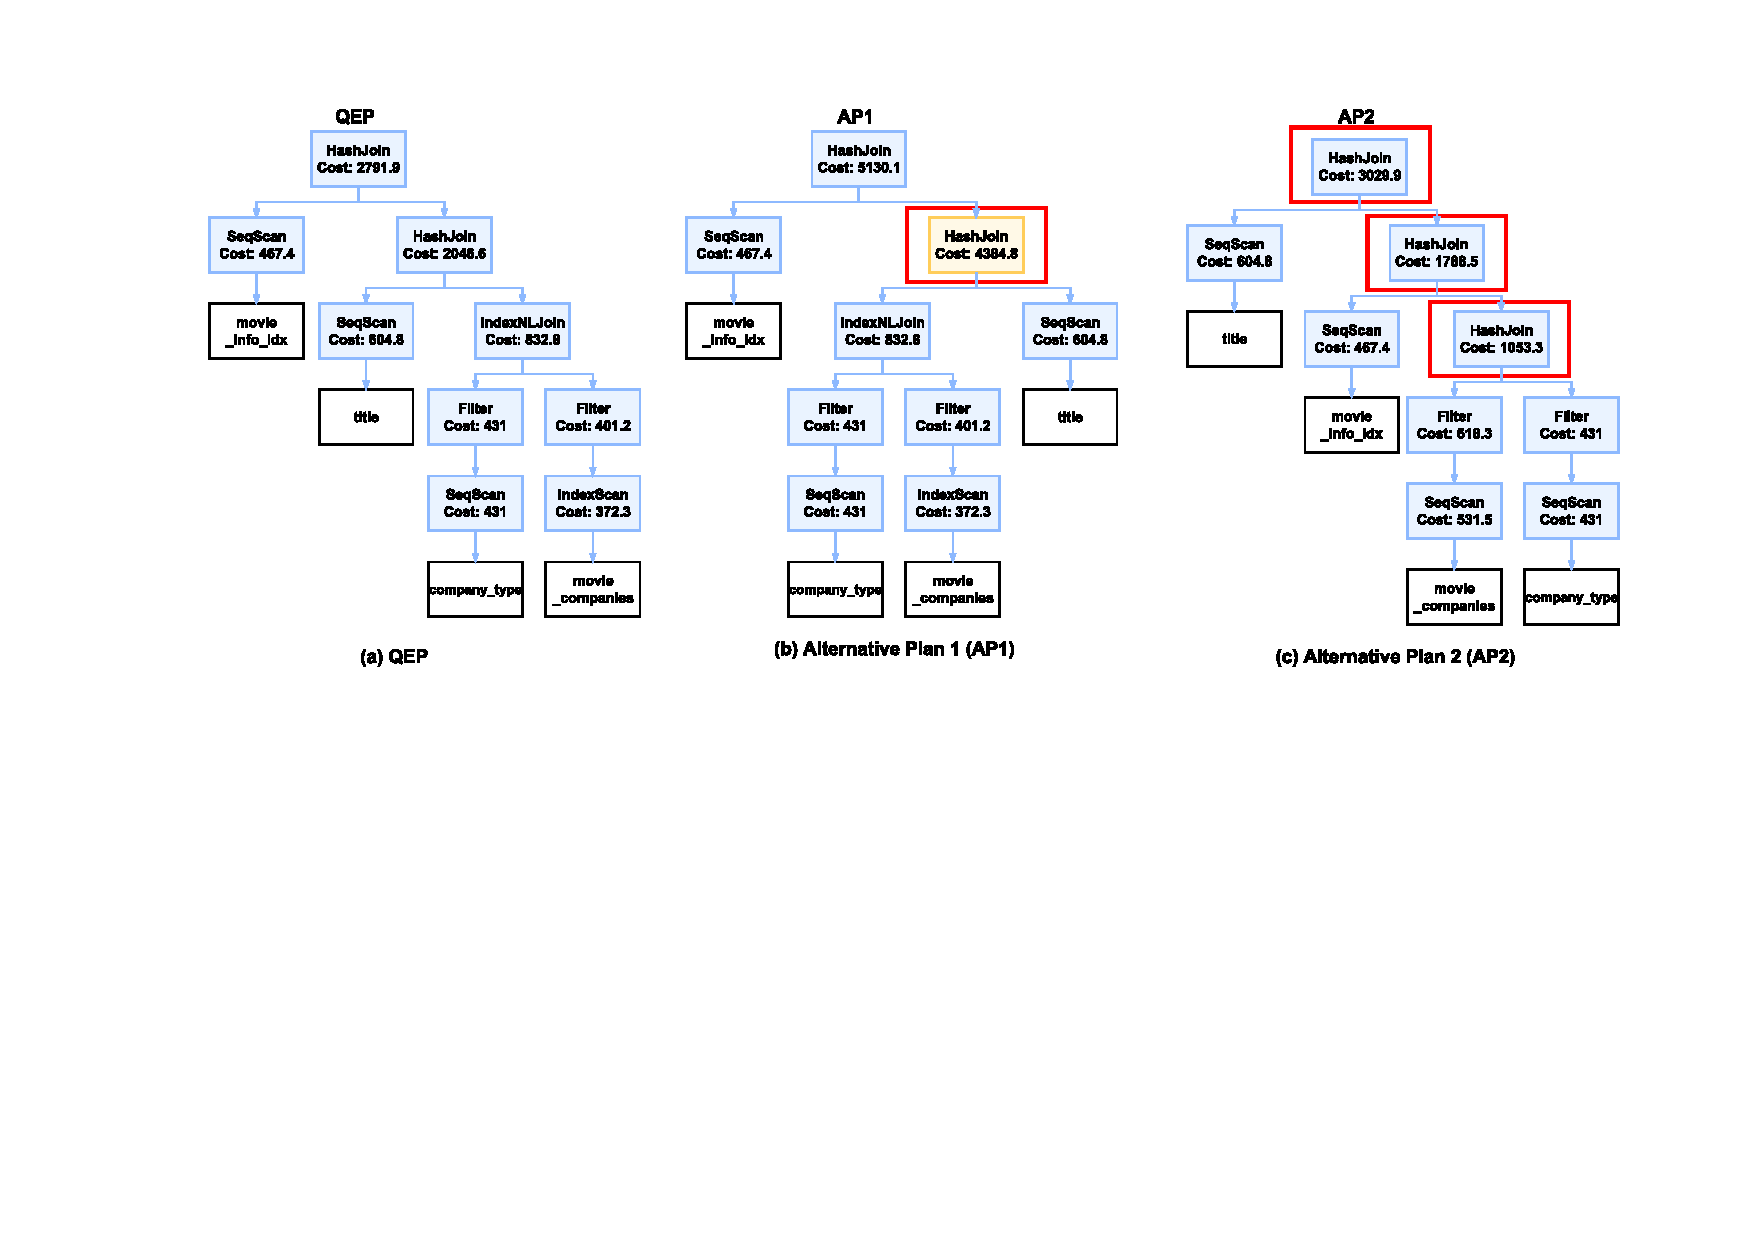
\includegraphics[width=0.95\linewidth]{motieg.pdf}
	\vspace{0ex}\caption{Examples of \textsc{qep} and alternative query plans.}
	\label{fig:alter_plans}
	%\hrule
	\vspace{0ex} \end{figure}

%====================================================================================================
\subsection{Understanding Query Execution Plans (QEPs)} \label{sec:nlg}
%====================================================================================================
A key goal of learning relational query processing is to understand  how \textsc{sql} queries are processed in an \textsc{rdbms} in practice. This can be achieved by understanding the content of the \textsc{qep} of a given query.  Major database textbooks (\eg \cite{dbtext,cow})  typically illustrate \textsc{qep}s of simple \textsc{sql} queries, their costs, and  adverse impact on estimated cost if alternative physical operators are chosen (\eg merge join instead of hash join) for a \textsc{qep}. However, they are not interactive and the variety of examples they can discuss is constraint by the page limit and cost. Hence, only a very few simple, static examples of \textsc{qep}s are typically exposed to learners.

Off-the-shelf \textsc{rdbms} (\eg PostgreSQL) provide the opportunity to greatly mitigate the limitations of textbooks. A learner may implement a database application in an \textsc{rdbms}, pose queries over it, and peruse the associated \textsc{qep}s to comprehend how they are processed by an industrial-strength query engine in practice. Such interactivity provides learners the freedom to formulate a large number of queries with diverse complexities and view the contents of corresponding \textsc{qep}s in real-time. 

Most existing \textsc{rdbms} expose the \textsc{qep} of an \textsc{sql} query using \textit{visual} or \textit{textual} (\eg unstructured text, \textsc{json}, \textsc{xml}) format.  Unfortunately, comprehending these semistructured textual formats to learn about query execution strategies of \textsc{sql} queries in practice can be daunting for learners. In contrast to natural language-based narrations in database textbooks, they are not user-friendly and assume deep knowledge of vendor-specific implementation details.  On the other hand, the visual format is relatively more user-friendly but hides important details. Consequently, in consistent with the \textit{Expectancy-Value Theory}, the task difficulty may become a barrier for some learners to learn about query execution strategies in a specific \textsc{rdbms} from these \textsc{qep} formats.  

\begin{example} \label{eg:1}
Doreen is an undergraduate student in a data science program who is currently enrolled in a database course. She wishes to understand the execution steps of the following \textsc{sql} query in PostgreSQL on the IMDb benchmark dataset~\cite{imdb} by perusing the corresponding \textsc{qep} in Figure~\ref{fig:plan}(a) (partial view). 
\begin{quote}
\begin{verbatim}
SELECT mc.note AS production_note, 
	   t.title AS movie_title, 
	   t.production_year AS movie_year
FROM company_type AS ct, 
	 movie_companies AS mc, 
	 movie_info_idx AS mi_idx, 
	 title AS t
WHERE ct.kind = 'production companies'
	  and mc.note like '%(co-production)%'
	  AND ct.id = mc.company_type_id
	  AND t.id = mc.movie_id 
      AND mc.movie_id = mi_idx.movie_id;
\end{verbatim}
\end{quote}
 Unfortunately, Doreen finds it difficult to mentally construct a narrative of the overall execution steps by simply perusing it. This problem is further aggravated in more complex \textsc{sql} queries. Hence, she switches to the visual tree representation of the \textsc{qep} as shown in Figure~\ref{fig:plan}(b). Although relatively succinct, it simply depicts the sequence of operators used for processing the query, hiding additional details about the query execution (\eg sequential scan, join conditions).  In fact, Doreen needs to manually delve into details associated with each node in the tree for further information.
\EndOfProof
\end{example}

Since natural language (\textsc{nl})-based narratives aided with visual examples (as in textbooks and lectures) have been the traditional mode of learning for decades, we advocate that an  intuitive natural language (\textsc{nl})-based description of a \textsc{qep} can greatly augment learning of the execution strategies of \textsc{sql} queries by an \textsc{rdbms}. The intuition is that \textsc{nl}-based descriptions may facilitate the flow state of learners (\textit{Flow Theory}) to the Goldilock's zone. This can then effectively complement the current visual tree format generated by existing  \textsc{rdbms}.  Specifically, a learner may either use the visual \textsc{qep} to get a quick overview and then peruse the \textsc{nl} description or study them in parallel to acquire detailed understanding. To support this hypothesis, we surveyed 62 and 56 unpaid volunteers taking the undergraduate database course in NTU in two semesters (2019 and 2020).  We use the \textsc{tpc-h} v2.17.3 benchmark  and a  rule-based natural language generation tool for \textsc{qep}s ~\cite{neuron} to generate natural language descriptions of \textsc{qep}s for \textsc{sql} queries formulated by the volunteers.  The volunteers were asked: \textit{``which query plan format they prefer for learning?''} 53.2\% and 55.4\% preferred \textsc{nl}-based description, respectively. Very few (3\% and 5.4\%, respectively) preferred the text format. Hence, there is clear evidence that learners prefer to use \textsc{nl}-based and visual tree-based formats for learning about \textsc{qep}.

\begin{figure}[t]
\centering
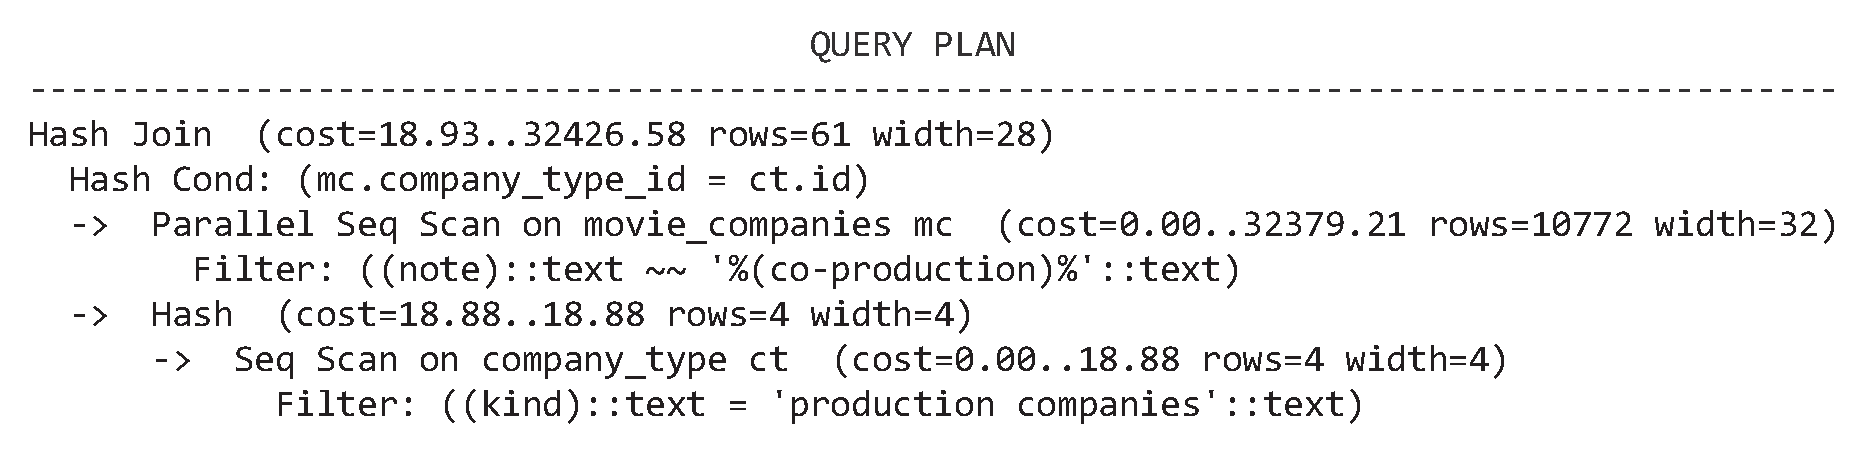
\includegraphics[width=0.45\linewidth]{newfig1.eps}
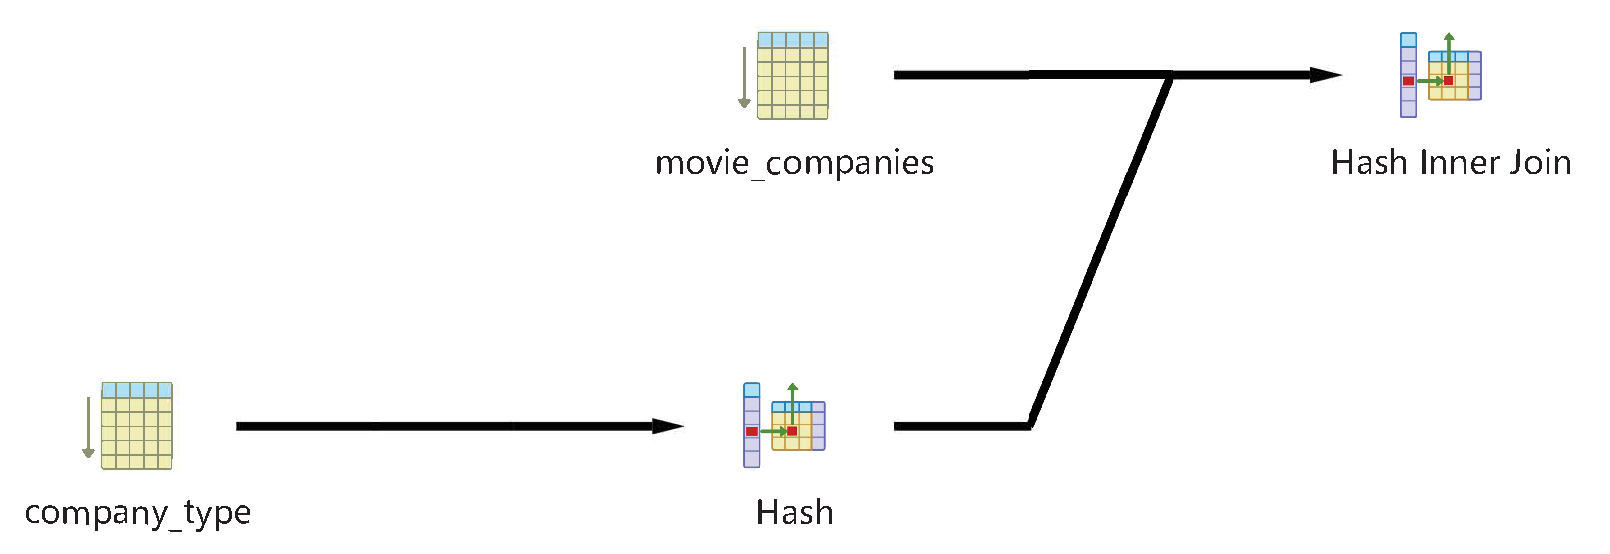
\includegraphics[width=0.5\linewidth]{sdf.eps}
\vspace{0ex}\caption{A \textsc{qep} in PostgreSQL and its visual tree representation.}
\label{fig:plan}
%\hrule
\vspace{0ex}\end{figure}


The majority of \textsc{nl} interfaces for \textsc{rdbms}~\cite{KS+20}, however, have focused either on translating natural language sentences to \textsc{sql} queries or narrating \textsc{sql} queries in a natural language. Scant attention has been paid for generating natural language descriptions of \textsc{qep}s~\cite{neuron,lantern}, which is a challenging problem.
Although deep learning techniques, which can learn task-specific representation of input data, are particularly effective for natural language processing, it has a major upfront cost. These techniques need massive training sets  of labeled examples to learn from. Such training sets in our context are prohibitively expensive to create as they demand database experts to translate thousands of \textsc{qep}s of a wide variety of \textsc{sql} queries.  Even  labeling using crowdsourcing is challenging as accurate natural language descriptions demand experts who understand \textsc{qep}s. Note that accuracy is critical here as low quality translation may adversely impact individuals' learning.

%====================================================================================================
\subsection{Learning Impact of Alternative Choices on QEP} \label{sec:impact}
%====================================================================================================
Natural language description of a \textsc{qep} enables a learner to understand the execution steps of a query. This may pique the interest of a learner to raise further questions related to query processing centred around a specific \textsc{qep}. Since major database textbooks typically discuss the adverse impact of choosing alternative physical operators or join ordering on the estimated cost, a learner may also like to delve deeper into the impact of these alternative choices on the estimated query processing cost of their queries.

\eat{This may be due to the shift from extrinsic motivation to intrinsic one to learn about relational query processing.}

\begin{example}  \label{eg:2} 
Reconsider Example~\ref{eg:1}. Doreen's course lectures and textbook discuss the impact of physical operator choices and join ordering  on the selection of a \textsc{qep}. Hence, after perusing the content of the \textsc{qep},  she wonders what will be the impact on the cost be if the hash join is replaced by a merge join? Is the estimated cost of the alternative query plan substantially higher compared to the \textsc{qep}? How much is the impact on the estimated cost if the join ordering is changed?   In this context, a narrative that explains why the \textsc{qep} is chosen by connecting its content with knowledge garnered from database textbooks will greatly benefit her learning. 
\EndOfProof
\end{example}

Unfortunately, as stated earlier, off-the-shelf \textsc{rdbms} are not developed for pedagogical support.  Typically, they do not expose the impact of alternative choices of various physical operators or join ordering on the \textsc{qep} in a \emph{user-friendly} manner to aid learning.  Note that such information is invaluable to learners as it not only facilitates hands-on inquire-driven learning on the impact of a choice of a physical operator  or a specific join ordering on the estimated cost of a \textsc{qep} but it also enables them to comprehend why a \textsc{qep} is chosen by the underlying \textsc{rdbms}. However,  an \textsc{rdbms} typically demands a learner to manually pose \textsc{sql} queries with various constraints on \textit{configuration parameters} (\textit{e.g.}, \texttt{enable\_hashjoin}, \texttt{enable\_nestloop} in PostgreSQL) to view the corresponding \textsc{qep} containing specific physical operators. Furthermore, one has to manually compare the generated plan with the original \textsc{qep} to understand the impact. Notably, a database course may not introduce these configuration parameters while exposing syntax and semantics of \textsc{sql}. It is also impractical to assume that learners will be familiar with them  when many are taking the course for the first time.  Clearly, based on the \textit{Expectancy-Value} and \textit{Flow} theories, a learner-friendly framework that can facilitate exploration of the impact of various physical operators and join ordering on a \textsc{qep} can greatly motivate learners to deeper engagement and learning of this topic. 

Intuitively,  given  an \textsc{sql} query and learner-specified \textit{preferences} (\eg merge join, index scan, specific join ordering), the goal is to automatically visualize the impact of these choices on the selected \textsc{qep}. In this context, it is important to generate a natural language-based explanation that goes beyond the conventional least-cost-based explanation to connect established knowledge related to usage scenarios of different physical operators from textbooks with the specified preferences. For instance, examples of some established knowledge are:  (a) index scan is the optimal access path for low selectivity whereas sequential scans perform better in high selectivity~\cite{borovicaGajic2018}; (b) merge join is preferred if the join inputs are large and are sorted on their join column~\cite{msdn}; (c) nested-loop join is ideal when one join input is small (\eg fewer than 10 rows) and the other join input is large and indexed on its join columns~\cite{msdn}. Such knowledge in the form of explanations will naturally facilitate learners' understanding of relational query processing. For instance, consider Example~\ref{eg:2}. Explanations such as (b) will help Doreen to understand why a hash join was chosen by the relational query engine.

The problem is challenging from several fronts. While under-the-hood it is straightforward to generate an \textsc{sql} query involving the learner-specified preferences and retrieve the corresponding \textsc{qep}, automatically generating appropriate visualization framework to aid learning is challenging. First, how should the results be presented in consistent with motivation theories to motivate learners to explore and learn? Note that a learner may want to view the impact of multiple physical operators and join ordering together instead of just a single operator or join ordering. Simply generating an \textsc{nl} description of the \textsc{aqp} is insufficient since this will demand a learner to manually compare the description of the original \textsc{qep} with it in order to understand the impact of various operators and join ordering. Naturally, this becomes tedious especially for complex queries.  Second, how can we generate  \textsc{nl} explanations that augment learning by connecting with textbook knowledge? It demands sophisticated text extraction, analytics, and summarization framework that connects the alternative query plans with relevant established knowledge embedded in online resources.   

%====================================================================================================
\subsection{Exploration of Informative Alternative Query Plans} 
%====================================================================================================
In the preceding challenge, a learner has clear preferences that they wish to explore with respect to a \textsc{qep}. However, this may not always be the case.  Some learners may not have clear idea of what alternative query plans they are interested in.\eat{ Consider the following example scenario.} 

\begin{example}\label{eg:3}
 Meng is another undergraduate student pursuing a degree in computer science and a classmate of Doreen in the database course. He also formulates the query in Example~\ref{eg:1}. After viewing the \textsc{qep}, he wonders what are the different alternative query plans (\textsc{aqp}s) considered by the underlying \textsc{rdbms} during the \textsc{qep} selection process. Specifically, are there alternative plan(s) that have similar (resp. different) structure and physical operators but very different (resp. similar) estimated cost? If there are, then how they look like? 
\EndOfProof
\end{example}


Off-the-shelf \textsc{rdbms} do not expose a \textit{representative} set of alternative query plans considered by the underlying query optimizer during the selection of a \textsc{qep} in a \emph{user-friendly} manner to aid learning. Hence, due to the lack of easy access to such information in \textsc{rdbms}, based on the \textit{Expectancy-Value Theory}, learners may restrict themselves to the simple and limited number of examples that are typically exposed in textbooks and lectures or simply abandon the effort. Clearly, a learner-friendly framework that can facilitate retrieval and exploration of ``informative'' alternative query plans associated with a given query can greatly aid in answering Meng's questions related to the query optimization process. 

Selecting a set of \textit{informative} \textsc{aqp}s to facilitate learning is a technically challenging problem. First, what is an ``informative'' \textsc{aqp} in the context of learning? To elaborate further, reconsider Example~\ref{eg:3}. Figures~\ref{fig:alter_plans}(b)-(c) depict two alternative plans for the query where the physical operator/join order differences are highlighted with red rectangles and significant cost differences are shown using yellow nodes. Specifically, \textit{AP1} has very similar structure as the \textsc{qep} but different join order involving \texttt{title} and \texttt{company\_type} relations and significantly different estimated cost. \textit{AP2}, on the other hand, displays similar estimated cost as the \textsc{qep}  but different join order. \textit{Which of these alternative plans should be revealed to Meng?} The overarching goal here is to  choose alternative plan(s)  that may enhance Meng's knowledge of the \textsc{qep} selection process (\ie informative) as well as motivate him to learn and explore. Certainly, any \textit{informativeness} measure needs to be cognizant of plans that a learner have already viewed for her query (including the \textsc{qep}) in order to avoid the exposure of highly similar information. It should also facilitate retrieval of plans that learners may be interested in as far as query optimization is concerned. Hence, it is paramount to take feedback from learners on the \textit{types} of \textsc{aqp}s that are potentially of interest to them and devise a mechanism to quantify \textit{informativeness} of a plan by mapping the knowledge acquired from the feedback to a \textit{utility} measure. Subsequently, we need to design techniques that can select informative plans that  \textit{maximize} the \textit{utility} as we cannot simply rely only on the estimated cost of alternative plans.  Second, the number of candidate \textsc{aqp}s for a given \textsc{sql} query is exponential in the worst case~\cite{SC98}. Hence, it is prohibitively expensive to scan all these plans to select informative ones. Note that the selection of \textsc{aqp} cannot be integrated into the plan enumeration step of the underlying query optimizer. We need to know the \textsc{qep} when computing \textsc{aqp} as they are selected with respect to the \textsc{qep} a learner has seen. 
	
At first glance, it may seem that we can select $k>1$ alternative query plans where $k$ is a value specified by a learner. Although this is a realistic assumption for many top-$k$ problems, learners may not necessarily be confident to specify the value of $k$ always. They may prefer to \textit{iteratively} view one plan-at-a-time and only cease exploration once they are satisfied with the understanding of the query optimization process for a specific query. Hence, $k$ may not only be unknown \textit{apriori} but also the selection of an \textsc{aqp} at each iteration to enhance learning of different plan choices depends on the plans viewed by a learner thus far. Clearly, it does not increase learners' understanding of the query optimization process or motivate them to use the framework if a plan with highly similar information of an already viewed plan is revealed to them in the subsequent iterations. This demands for a flexible solution framework that can select informative \textsc{aqp}s in absence or presence of the $k$ value. 


%====================================================================================================
\subsection{Understanding Cost Estimation of a Physical Query Plan}  \label{sec:cost}
%====================================================================================================
The preceding subsections introduce research issues that aim to facilitate learning of the execution strategy of an \textsc{sql} query and  interesting plan choices a relational query optimizer makes in practice. Another key knowledge that a learner needs to acquire is the cost estimation procedure of these plans.   

\begin{example}\label{eg:4}
 Doreen and Meng have learnt from textbooks and lectures how the cost of a physical query plan can be estimated. However, the number of queries considered in these modes of learning and their complexities are limited. They are motivated to experience cost estimation of plans associated with a wider variety of queries. Hence, they pose several queries with different degrees of complexity on the IMDb dataset in PostgreSQL. They can view the overall estimated cost of a \textsc{qep} as well as cost of different subtrees (\eg Figure~\ref{fig:alter_plans}). However, they cannot view step-by-step details of the input parameters and the formulas used by the underlying query optimizer to compute these numbers. For instance, in Figure~\ref{fig:alter_plans}(a), why is the cost of the first \texttt{HASH JOIN} \textit{2046.6}? By undertaking a back-of-the-envelope calculation using formulas learnt in the course, they could not replicate this value. Are some of the principles and formulas to compute cost different from what they have learnt from textbooks and lectures? If so, then why? 
 
 Doreen and Meng also wonder what the intermediate result sizes of different operations are here? When they execute one of the queries, they have to wait for a considerable amount of time to view the results. Does the estimated time cost of the \textsc{qep} differ significantly from the actual cost? Why? 
\EndOfProof
\end{example}

Existing \textsc{rdbms} do not provide any learner-friendly support to facilitate such learning. Consequently, based on motivation theories, learners may not pursue this direction of inquiry using an \textsc{rdbms}, surrendering valuable opportunity for hands-on acquisition of knowledge of the cost estimation process. It is challenging, however, to expose an interface to facilitate such learning and exploration. First, it demands automated analysis of the code base of the underlying query optimizer to extract various formulas used for cost estimation. These formulas may not necessarily be identical across all \textsc{rdbms} or textbooks. For instance, in~\cite{dbtext}, the cost of a selection involving inequality condition is approximated to be 1/3 of the input size independent of the selection condition. On the other hand, in~\cite{cow}, more accurate measure is used for estimating the selection cost.  Furthermore, a specific \textsc{rdbms} may implement variants of these formulas. Second, it is paramount to connect these formulas with specific input parameters for a query to reveal how the cost of a plan is estimated while emphasizing the similarity and differences with textbook knowledge. A framework that can support this in a palatable manner to facilitate learning is non-trivial as it may demand a sophisticated natural language generation framework that connects analysis of the code base with textbook content. Third, superior visualization and \textsc{nl}-based framework are necessary to explain to learners the reasons for the differences in estimated and actual cost of a query. Although tools such as~\cite{picasso} allow one to visualize the cost of different plans over the plan space,  they are not designed for explaining the \emph{cost differences} for a \emph{specific} query in a palatable manner. 

%====================================================================================================
\subsection{A Unifying Framework: Chatting with a Relational Query Engine} 
%====================================================================================================

\begin{figure}[t]
\centering
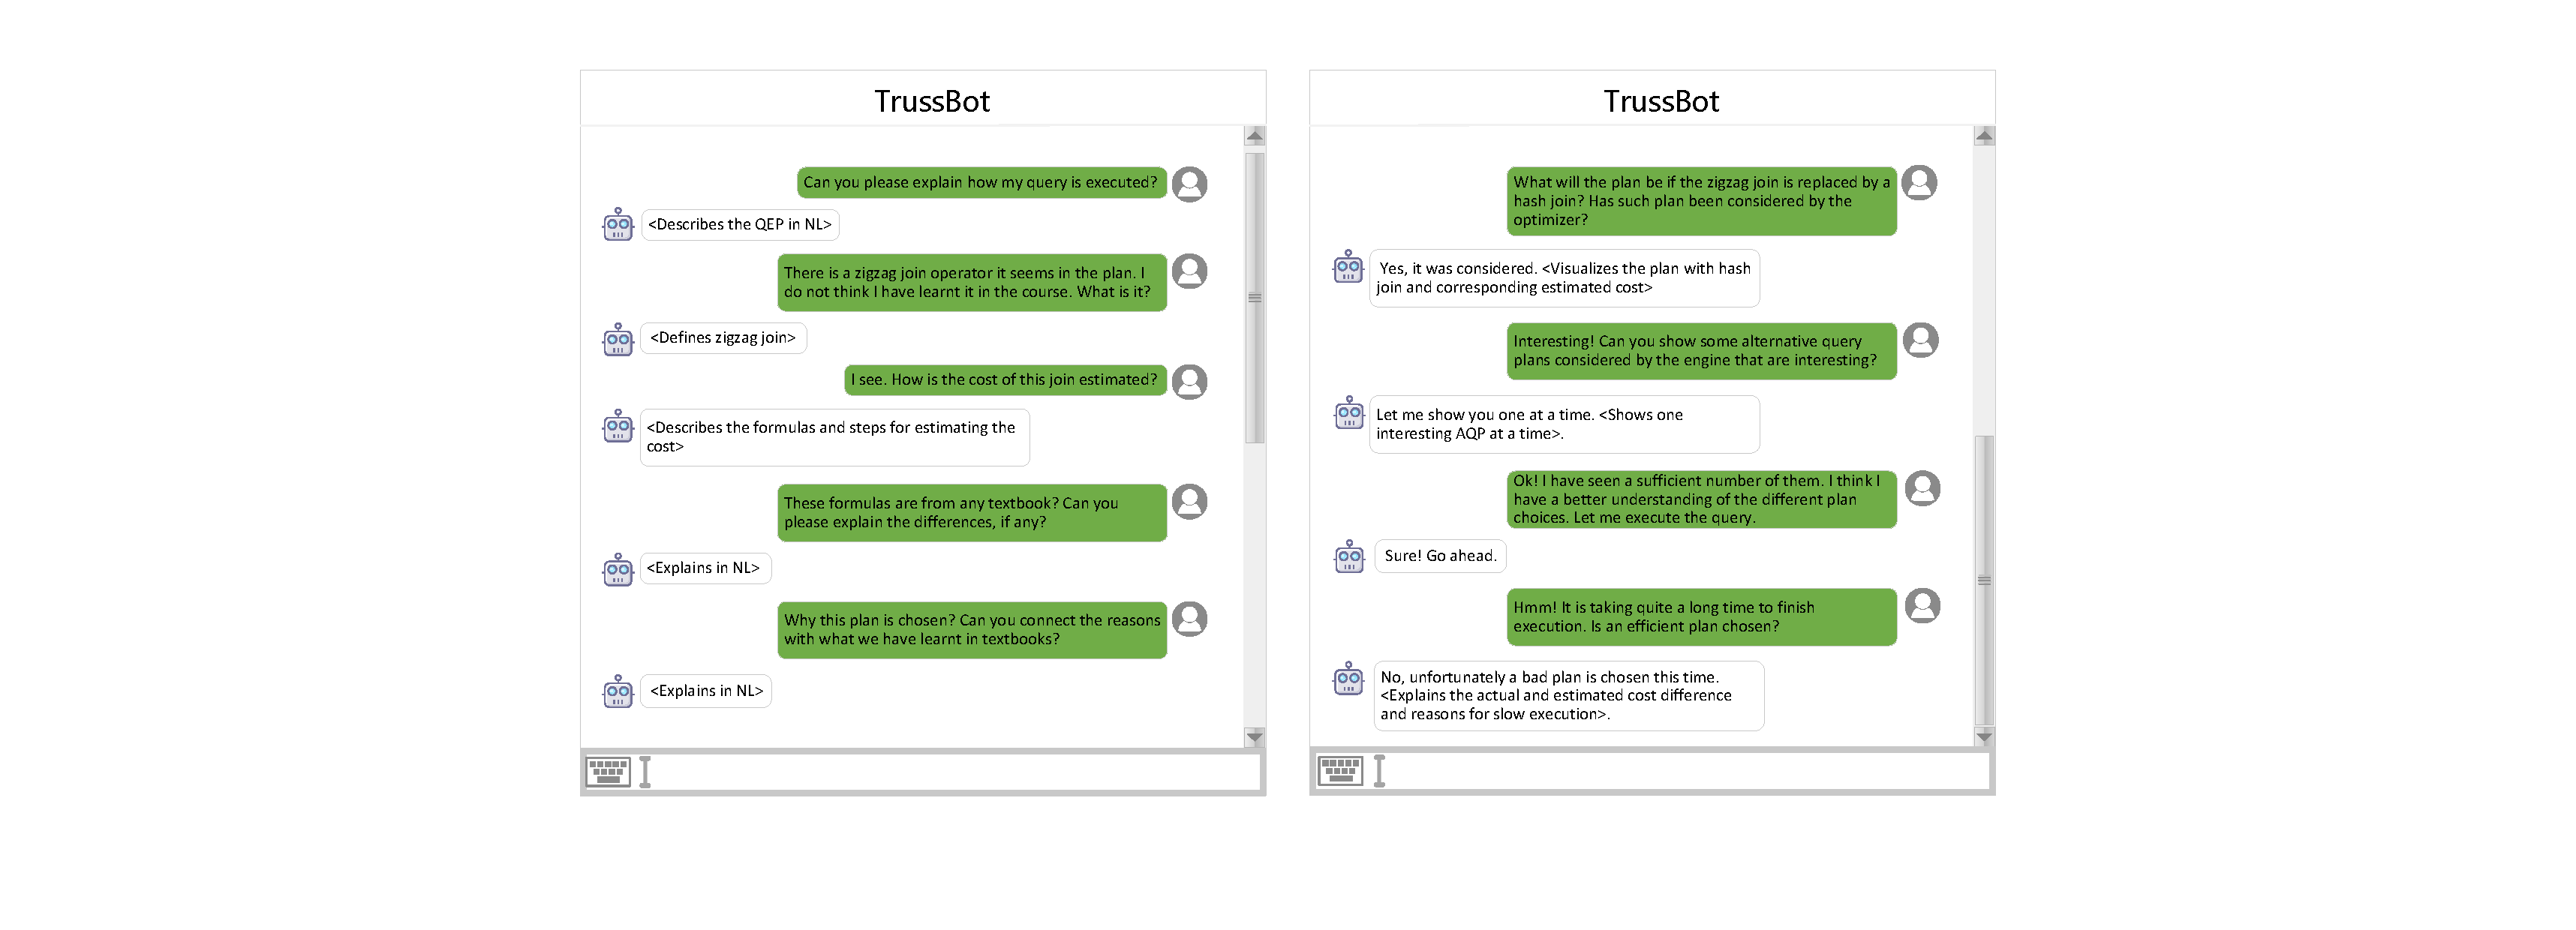
\includegraphics[width=\linewidth]{chatbot.pdf}
\vspace{0ex}\caption{An example of interaction between a learner and the chatbot.}
\label{fig:chatbot}
%\hrule
\vspace{0ex}\end{figure}

Although addressing the aforementioned issues has the potential to facilitate learning of relational query processing by providing learner-friendly platforms, a set of isolated platforms that address these different issues will make it cumbersome for learners to navigate and take advantage of them.  For instance, learners may find it overwhelming to operate three independent technology-enabled learning platforms targeting \textsc{nl} description generation of \textsc{qep}, exploration of \textsc{aqp}, and cost analysis of query plans, respectively. This may deter them to use such technology for learning. Given that young adults often interact through chat apps (\eg Whatsapp, WeChat), a natural language interaction framework (\ie chatbot) that can unify these solutions may bring practical benefits to learners.  A possible interaction between a learner and a hypothetical chatbot designed for interacting with a relational query engine are shown in Figure~\ref{fig:chatbot}.

Building a high-quality chatbot for a relational query engine to facilitate learning is non-trivial and challenging.  In addition to the challenges mentioned earlier for addressing individual components, a chatbot brings new challenges with respect to correct parsing and interpretation of a learner's statement, constructing correct (syntactically and semantically) responses in a natural language, engaging learners in conversations, and so on. While these challenges are long recognized in building a generic chatbot~\cite{GGL18}, the domain-specific nature of the problem brings in interesting flavor to it. Different from natural conversations, a learner’s questions usually have concrete objectives, actively requesting information, and an answer to every question should facilitate understanding of relational query processing. Furthermore, a learner's questions at each step are not only closely related to the chatbot’s current answers, but also need to take into account the context of the previous parts of the conversation. For example, consider the first three questions in Figure~\ref{fig:chatbot} from the learner. These questions are actively requesting information related to relational query processing. Observe that the third question is related to the preceding parts of the conversation.  

Any chatbot needs to consider two kinds of information in a learner's question: (1) the intent of the question (\eg understanding cost computation) and (2) the content of the question (\eg cost computation steps of zigzag join in a \textsc{qep}).  To this end, we can construct a \textit{query processing knowledge graph} semi-automatically to represent a collection of relational query processing concepts. Then the intent and content can be determined by \textit{mapping} the question to different concepts in the knowledge graph. Note that similar idea of knowledge graph has been recently exploited in the context of question generation for multi-party court debates for judicial education~\cite{ZJ+22}. Once the intent and content of a question are determined, the chatbot invokes the relevant component (Section~\ref{sec:nlg}-\ref{sec:cost}) to retrieve the answer for the specific question. The result returned by it is then \textit{transformed} into a natural language (supported by visual representations, if necessary) and presented to the learner.

   

  \begin{table*}[t]
\centering
 \caption{\label{tab:learn}Learning-centric issues.}
 \scriptsize
 \begin{tabular}{|p{70mm}|p{77mm}|}
  \hline
  \textbf{Issue} & \textbf{Questions to address}  \\
  \hline
 \textbf{ \textit{Rational for the impact of technologies on learning}} & Will learners work more efficiently, more effectively, more intensely? \\
 & Will the technology help them to learn for longer, more deeply, more productively? \\ \hline
\textbf{\textit{Role of technology in learning}} & Will it help learners to gain access to learning content? \\
& Will the technology provide feedback?\\ \hline
 \textbf{\textit{Technology should support effective interaction for learning}} & Does it support effective interaction with learners?\\ \hline
 \textbf{\textit{Identify what learners will stop doing}} & What it will replace or how the technology activities will be additional to what learners would normally experience?\\
  \hline
 \end{tabular}
\end{table*}
 
%====================================================================================================
\subsection{Learning-centric, Generic, and Psychology-Awareness of Solutions}  \label{sec:issue}
%====================================================================================================
In addition to the challenges within each aforementioned issues, any solution to them must ensure the following features.

\begin{itemize} \itemsep = -0.5ex

\item \textbf{Learning-centric.} The role, impact, and interaction of the platforms designed to address aforementioned issues have to be learning-centric, \ie they bring about improvement in learning. Table~\ref{tab:learn} lists the learning-centric issues~\cite{HXK12} that any technology-enabled solution needs to address. For instance, consider the last issue. An effective solution to \textsc{nl} descriptions of \textsc{qep}s will provide learners an additional interface to learn about query execution strategies to what they would normally experience. Similarly, consider the second issue. A solution to user-friendly exploration of \textsc{aqp}s will enable learners to gain easy access to informative plans to aid learning of the query optimization process. 
 
\item \textbf{Generalizability.}  Solutions must be \textit{generalizable} to different \textsc{rdbms} and applications. This will significantly reduce the cost of its deployment in different learning institutes and environments where different application-specific examples and \textsc{rdbms} may be used to teach database systems. For example, the natural language generation framework should be generalizable.  Ideally we would like to generate natural language descriptions of \textsc{qep}s using one application-specific dataset (\eg movies) and then use it for other applications (\eg hospital) on any off-the-shelf \textsc{rdbms}. 

\item  \textbf{Psychology-awareness.} Any technology-enabled learning framework has to be \textit{learner-centric}, \ie it has to be cognizant of the psychology of learners. Any deployable  solution has to be palatable and engaging to learners so that they are motivated to learn and explore. Hence, these solutions need to be consistent with various cognitive psychology and motivation theories to have practical impact. For example, the \textsc{nl} descriptions for different queries must not use the same language to describe various operations in \textsc{qep}s. Similarly, highly similar \textsc{aqp}s should not be exposed to the learners. Otherwise, learners may feel bored after viewing several \textsc{aqp}s or reading the \textsc{nl} descriptions for several queries. In fact, this is consistent with research in psychology that have found that repetition of messages can lead to annoyance and boredom~\cite{CP79} resulting in purposeful avoidance~\cite{HK13}, content blindness~\cite{HG+11}, and even lower motivation~\cite{SPC90}.
\end{itemize}


%====================================================================================================
\subsection{Towards Data-driven Education} 
%====================================================================================================
As remarked in Section 1, learning can be facilitated  by education. Hence, technological platforms that address the aforementioned challenges may pave the way for \emph{data-driven} education due to rich access to \textit{interaction log} data of learners.  Such log data may consists of access times of learners, history of queries formulated by learners, temporal information related to various interactions, among others. This provides a rich data source for building data-driven techniques to facilitate education by analyzing these data at both individual and group levels and correlating them with the performances of learners in tests (\ie academic outcomes).  A non-exhaustive list of questions that can be answered by exploiting the log data to facilitate data-driven education is as follows:

\begin{itemize} \itemsep = -0.5ex

\item How do the type and complexity of \textsc{sql} queries posed by learners evolve over time? What are the activity patterns of learners during a semester? Answers to these questions may provide insights on motivation and learning habits of learners.  

\item How do learners learn relational query processing? Numerous studies in cognitive psychology show that \textit{spacing} (\ie distributing practice over more sessions) significantly improves long-term learning compared to \textit{massing} (\ie practice in longer sessions)~\cite{BB11,BDK13,SB15,TR10}. The interaction data may enable us to build models to predict learners demonstrating massing, thereby enabling timely intervention to nudge them to more effective learning habits.

\item Research in education posits that technology can be used effectively as a short but focused intervention to improve learning especially when there is regular and frequent usage over a period of several weeks~\cite{HXK12}. In our context, it is expected that the platforms are also for focused usage over a period of few weeks. Do they help learners to perform better in tests and coursework? Is there any correlation between frequency of engagement with a platform and performance? Answer to this may provide data-driven insights to the effectiveness of these tools in learning. 

\item Do learners continue to use the platforms even after the end of a database course? This may indicate intrinsic motivation to learn relational query processing. 

\item Can the queries posed by learners over time shed light on the difficulties they face with respect to the learning and understanding of relational query processing and optimization? Answer to this question may facilitate the design of more effective and efficient pedagogical strategies to improve effectiveness of teaching.


\end{itemize} 

In summary, addressing the aforementioned research issues provide us a unique opportunity to take a data-driven approach to the education of relational query processing that may otherwise be infeasible through traditional mode of teaching.

\begin{figure}[t]
\centering
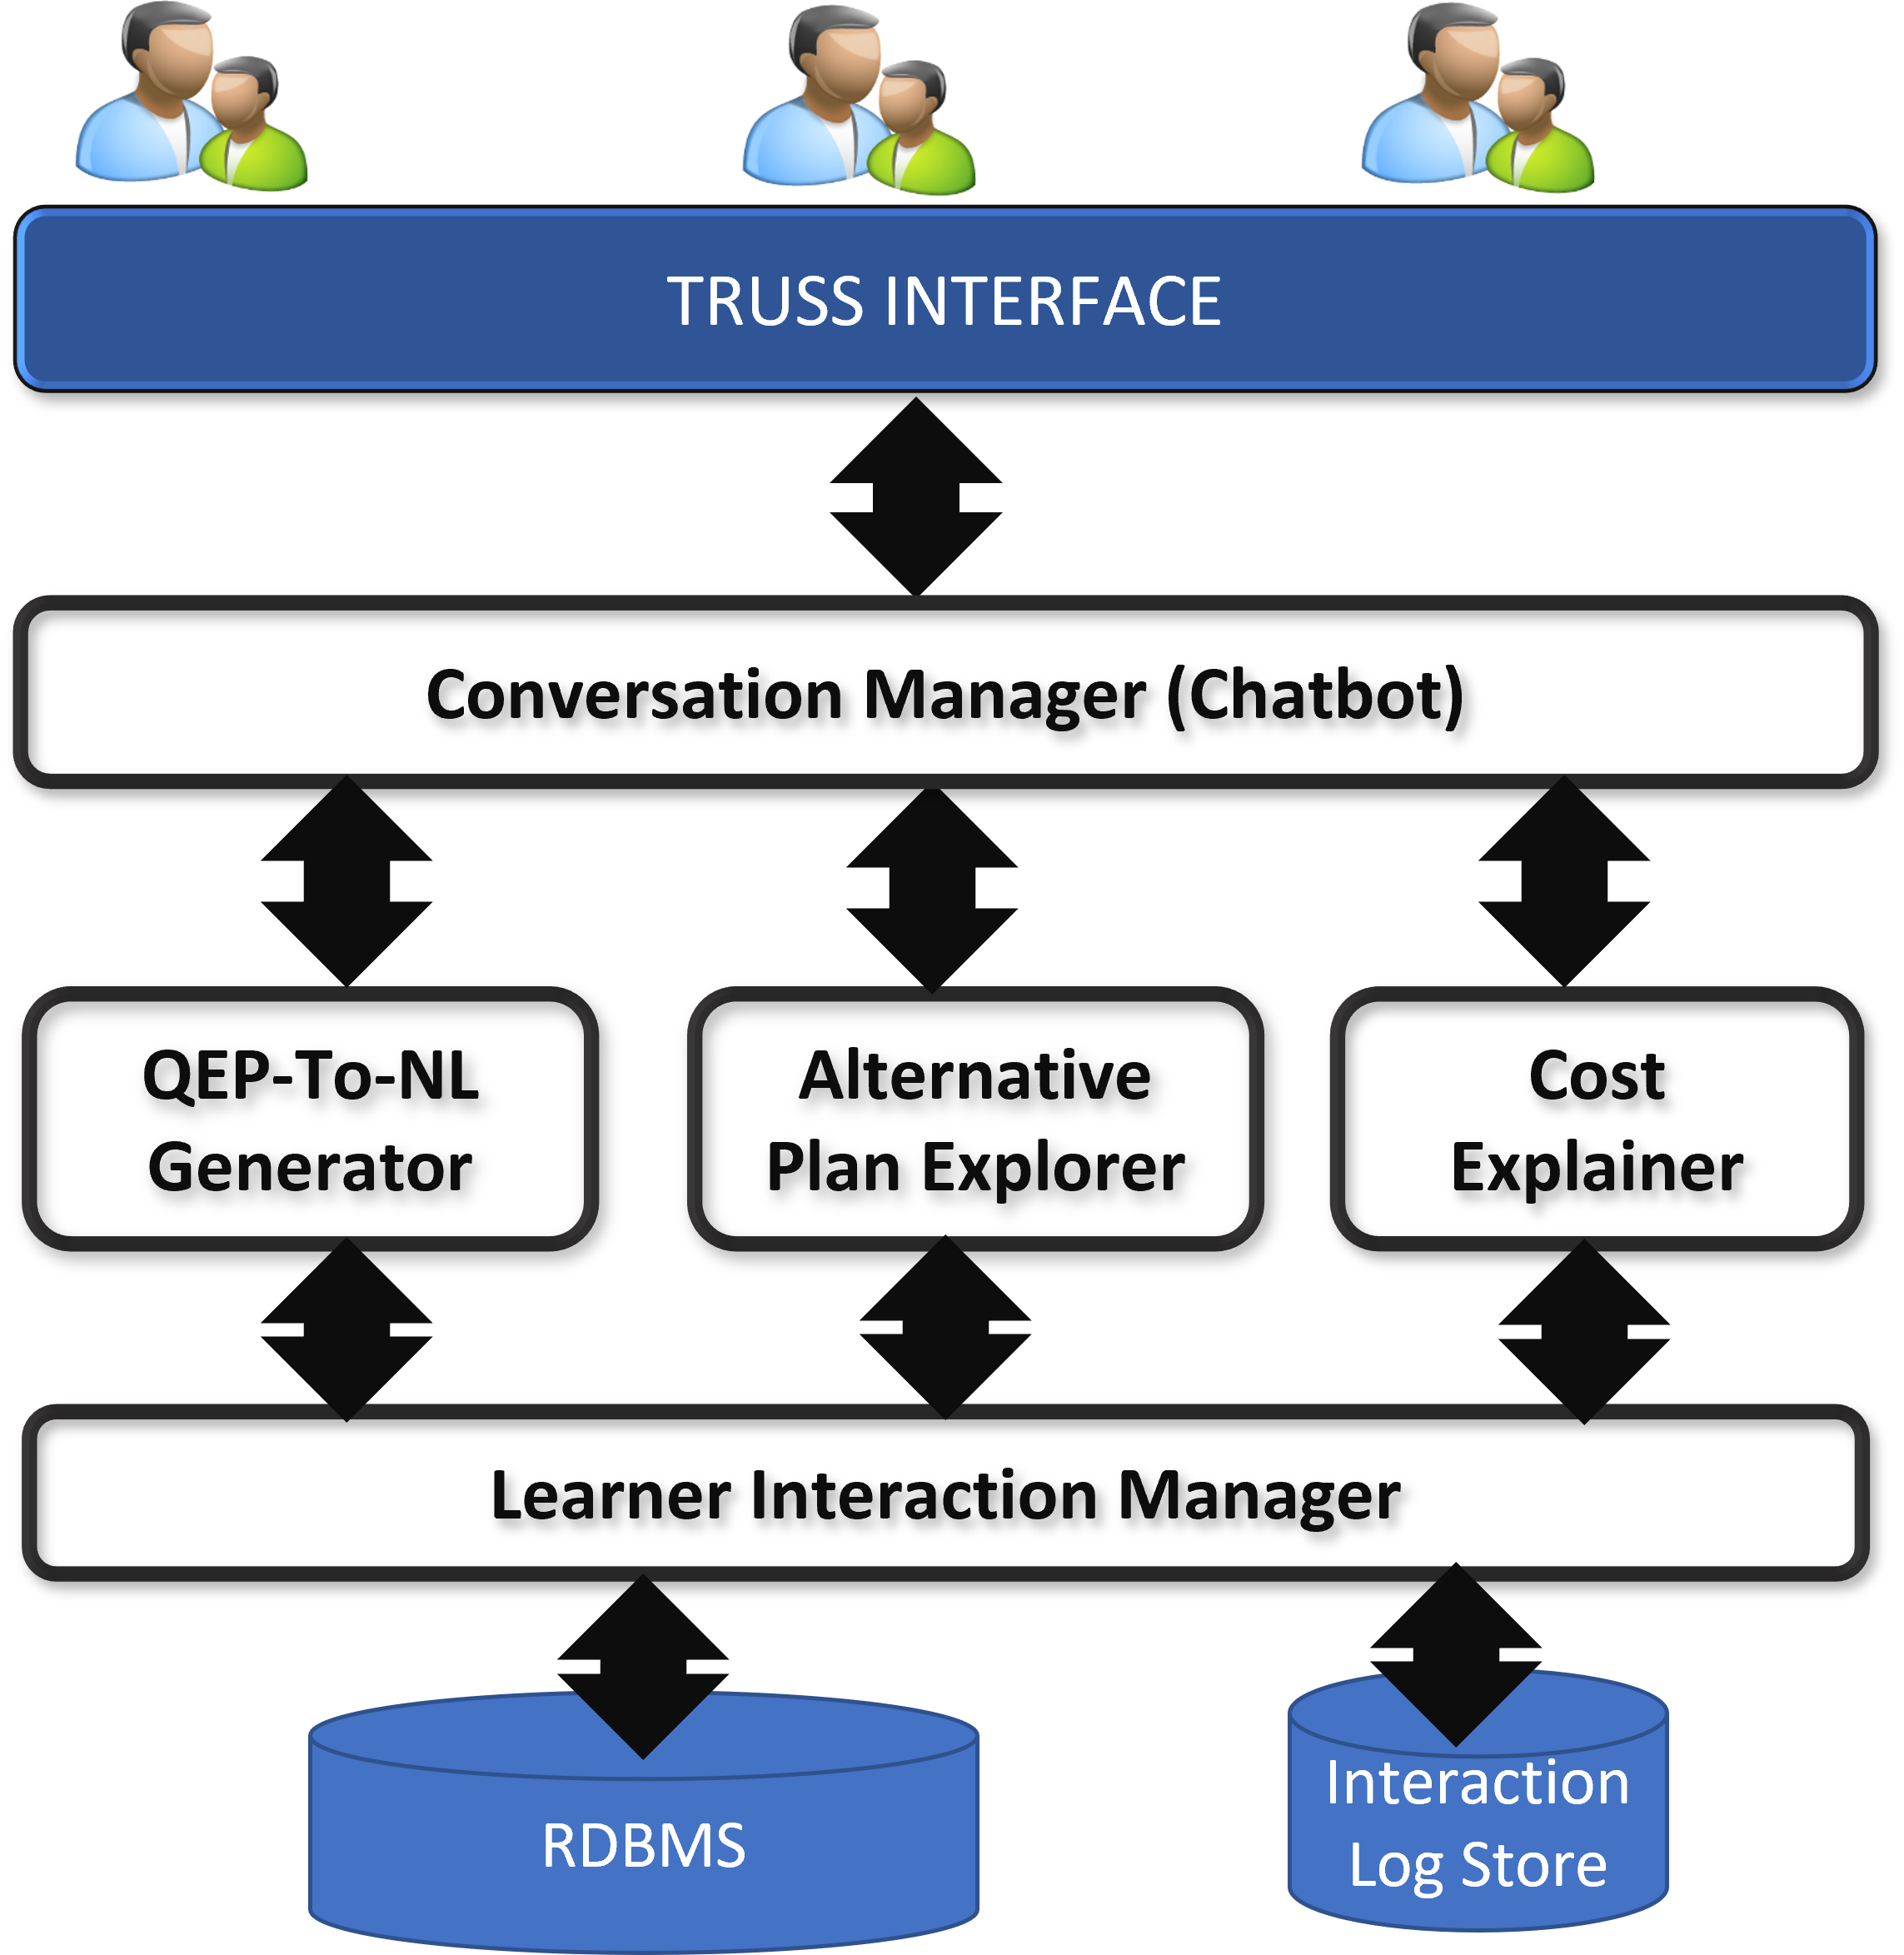
\includegraphics[width=0.4\linewidth]{truss.png}
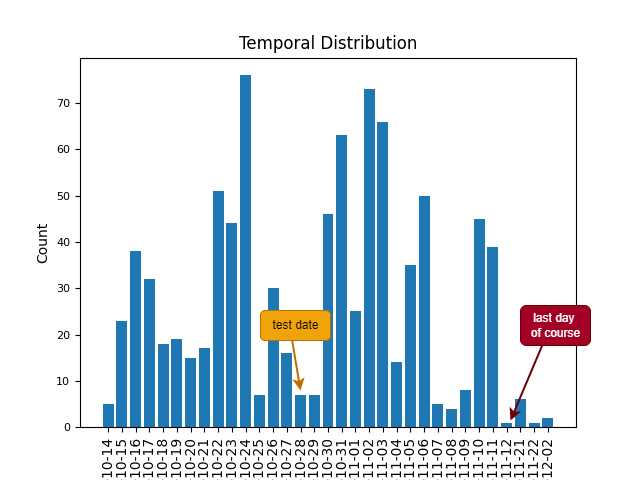
\includegraphics[width=0.5\linewidth]{neuron-time.png}
\vspace{0ex}\caption{(a) Architecture of \textsc{truss} (left); (b) No. of queries versus time (right).}
\label{fig:neuron}
%\hrule
\vspace{0ex}\end{figure}


%====================================================================================================
\section{The TRUSS System}  
\label{sec:truss}
%====================================================================================================
 Figure~\ref{fig:neuron}(a) depicts the high-level architecture of the \textsc{truss} (\textbf{T}echnology-enabled Lea\textbf{R}ning of Q\textbf{U}ery Proce\textbf{SS}ing) system that we are currently building to address the challenges introduced in the preceding section.  The \textit{QEP-to-NL Generator}, \textit{Alternative Plan Explorer}, and \textit{Cost Explainer} components aim to address the challenges in Sections 3.2, 3.3 \& 3.4, and 3.5, respectively. The \textit{Conversation Manager} is to realize the unifying chatbot (Section 3.6) and the \textit{Learner Interaction Manager} is responsible to facilitate data-driven education (Section 3.8). In this section, we briefly describe our recent efforts to build three frameworks, \textsc{neuron}~\cite{neuron} and \textsc{lantern}~\cite{lantern-demo}, that aim to address the problem described in Section~\ref{sec:nlg} (\ie \textit{QEP-to-NL Generator}), and \textsc{mocha}~\cite{mocha} that takes an initial step to address the problem in Section~\ref{sec:impact} (\ie  \textit{Alternative Plan Explorer}).  The reader may refer to~\cite{neuron,lantern,lantern-demo,mocha} for details on these frameworks.
%====================================================================================================
\subsection{NEURON and LANTERN} %17
%====================================================================================================
\textsc{neuron}~\cite{neuron,neuron-soft} is the first system that exploits a rule-based interpretation engine to generate \textsc{nl} description for \textsc{qep} in PostgreSQL.  Specifically, given the \textsc{qep} of a \textsc{sql} query, \textsc{neuron} first parses and transforms the \textsc{qep} of an \textsc{sql} query into an operator tree where each node contains relevant information associated with a plan (\eg filter conditions). Next, it traverses the tree and generates a \textsc{nl} description of the node based on \textsc{nl} templates and the information it carries.  It also supports a preliminary \textit{natural language question answering}  system that allows a user to seek answers to a variety of concepts and features associated with a \textsc{qep}. 

\textsc{neuron} is a rule-based framework that is tightly integrated with PostgreSQL. Hence, it is not generalizable (Section~\ref{sec:issue}).  \textsc{lantern}~\cite{lantern,lantern-demo,lantern-soft} addresses this limitation by not only making the solution generalizable but also psychology-aware. It incorporates a \textit{declarative framework} called \textsc{pool} to empower \textit{subject matter experts} (\textsc{sme}s) create and manipulate the \textsc{nl} descriptions (\ie labels) of physical operators, which are the building blocks of \textsc{qep}s. The data definition in \textsc{pool} allows one to declaratively create physical operator objects associated with a specific \textsc{rdbms}. For example, one can create the definition of hash join operator in PostgreSQL (\texttt{pg}) as follows.

\begin{quote}
\begin{verbatim}
CREATE POPERATOR hashjoin FOR pg
(ALIAS = null,
TYPE = 'binary',
DEFN = null,
DESC = 'perform hash join',
COND = 'true',
TARGET = null)
\end{verbatim}
\end{quote}

In particular, the \texttt{TYPE} attribute can take either \textsf{`unary'} or \textsf{`binary'} value. The \texttt{DESC} attribute allows one to specify a natural language description of the operation performed by the operator.   The \texttt{COND} attribute takes a Boolean value to indicate whether a specified condition (\eg join condition) should be appended to the natural language description of an operator. Values of all attributes are taken from the atomic type \texttt{string} (possibly empty). Note that no relation or condition is specified in \texttt{DESC}. This is because these are added automatically to \texttt{DESC} by exploiting \texttt{TYPE} and \texttt{COND} attributes  of an operator. For instance, since \texttt{TYPE} is \textsf{`binary'} in the above definition, two variables representing join relations will be added automatically to the description of \texttt{hashjoin}.  Lastly, the \texttt{TARGET} attribute allows one to specify the operator name which is supported by the defined operator. For example, \texttt{TARGET} is set to \textsf{`hash join'} for the definition of \texttt{hash} operator.


The key goals of the data manipulation component of \textsc{pool} are to provide syntactical means to support (a) retrieval of specific properties (\ie attributes) of physical operators using \textsc{sql}-like \texttt{SELECT-FROM-WHERE} syntax, (b) generation of the \textit{template} for natural language description of  an operator using the \texttt{COMPOSE} clause, and (c) update properties of physical operator objects using  \texttt{UPDATE} and \texttt{REPLACE} clauses. Specifically, the \texttt{COMPOSE} clause uses the \textit{desc}, \textit{type}, and \textit{cond} attributes of operators to generate the template. For example, the template generation for the \texttt{hash} operator can be specified as follows.
\begin{quote}
\begin{verbatim}
COMPOSE hash FROM pg
\end{verbatim}
\end{quote}

The above statement will return the template \textit{``hash \$$R_1$\$''}, which can be subsequently used by \textsc{lantern} to generate specific description of the \texttt{hash} operator in a \textsc{qep}. Also, observe that $R_1$ is appended based on the \textit{type} attribute of the \texttt{hash} object. An example to generate the \textsc{nl} description template of the \texttt{hash join} operator is as follows.
\begin{quote}
\begin{verbatim}
COMPOSE hash, hashjoin FROM pg
USING hashjoin.desc = 'perform hash join'
\end{verbatim}
\end{quote}
The above statement generates the following template: \textit{``hash \$$R_1$\$ and perform hash join on \$$R_2$\$ and \$$R_1$\$ on condition \$$cond$\$''}. 

The update statement can be exploited to assign definition or description of an operator from one commercial database to another, thereby making it more efficient for an \textsc{sme} to specify properties of physical operators. The following example demonstrates how the description of hash join in PostgreSQL is transferred to the hash join operator in DB2.

\begin{quote}
\begin{verbatim}
UPDATE db2
SET desc = (SELECT desc
 FROM pg WHERE pg.name = 'hashjoin')
WHERE db2.name = 'hsjoin'
\end{verbatim}
\end{quote}

It can also be used along with the \texttt{REPLACE} clause to transfer definition or description of an operator object to another within the \emph{same} source. For example, one can transfer the description of hash join to nested loop join by replacing the word \textsf{`hash'} with \textsf{`nested loop'} as follows.

\begin{quote}
\begin{verbatim}
UPDATE pg
SET desc = REPLACE((SELECT desc FROM pg AS pg2
WHERE pg2.name = 'hashjoin'), 'hash', 'nested loop')
WHERE pg.name = 'nested loop join'
\end{verbatim}
\end{quote}

Note that the \texttt{REPLACE} clause takes three parameters as input, namely, the description or definition of an operator object, the string in it that needs to be replaced (\eg \textsf{`hash'}), and its new replacement string (\eg \textsf{`nested loop'}).

Once the physical operator objects for different \textsc{rdbms} are created in \textsc{pool} and stored, the physical operator tree of a given query in any \textsc{rdbms} can be augmented by automatically annotating relevant nodes with \textsc{nl} descriptions by leveraging the \texttt{COMPOSE} statement and replacing the place holders in \textsc{nl} templates with specific relations, attribute names, and predicates relevant to the query.  The \textsc{nl} description generation framework then utilizes this augmented operator tree and \textit{integrates} a rule-based and deep learning-based techniques. In particular, the latter infuses language variability in the descriptions opportunely. This strategy has been shown to mitigate the impact of boredom on learners that may arise due to repetitive statements in different \textsc{nl} descriptions~\cite{lantern}.
%====================================================================================================
\subsection{MOCHA} %17
%====================================================================================================
\textsc{mocha} (i\underline{M}pact of \underline{O}perator \underline{CH}oices visu\underline{A}lizer)~\cite{mocha, mocha-soft} aids learner-friendly interaction and visualization of the impact of alternative physical operator choices on a selected \textsc{qep} for a given \textsc{sql} query. It is built on top of PostgreSQL. Given  an \textsc{sql} query and learner-specified \textit{operator preferences} (\eg merge join, index scan), \textsc{mocha} automatically visualizes the impact of these choices on the selected \textsc{qep}.
Specifically, it exploits the \textit{planner method configuration}\footnote{\scriptsize \url{www.postgresql.org/docs/9.2/runtime-config-query.html\#RUNTIME-CONFIG-QUERY-CONSTANTS}.} feature of PostgreSQL to generate \textsc{aqp}s based on a user input. The configuration parameters in this feature provide a way to enforce the query optimizer to choose a query plan with certain user-specified physical operators. By default, all parameters are turned on during query processing. A query request is sent to PostgreSQL using the default settings to retrieve the \textsc{qep} of a query. 

In order to retrieve \textsc{aqp}s, a learner may select a subset of the configuration parameters (through a user-friendly visual interface) based on the physical operators that she intend to view in these plans. In this case, the corresponding parameters are set to \textsf{``true"} (\eg \texttt{SET enable\_mergejoin = \textsf{true}}) in the query request. \textsc{mocha} supports two modes for generating alternative plans, namely, \textit{single mode} and \textit{multiple mode}.  In the former mode, \textsc{mocha} sends a query request to PostgreSQL in which the \emph{unselected} parameters are set to \textsf{``false''} to generate an \textsc{aqp} containing the operators corresponding to the selected parameters that are relevant to the processing of the query. In the latter mode, every selected parameter is either set to \textsf{``true''} or \textsf{``false''} to create all possible combinations of these parameters. \textsc{mocha} iterates through these combinations and sends corresponding query requests to PostgreSQL. It only maintains all \emph{distinct} plans retrieved from these requests. To facilitate learning, it provides a learner-friendly \textsc{gui} to detect and visualize various structural and cost differences between a selected \textsc{aqp} and the \textsc{qep}. 

\textsc{mocha} also generates a natural language-based explanation that goes beyond the conventional least-cost-based explanation to connect established knowledge related to usage scenarios of different physical operators that a learner has learnt from textbooks with the operators in a \textsc{qep}. The current version manually extracts usage scenarios of different physical operators from the relevant literature. This is feasible since there is a small number of physical operators in PostgreSQL. Then a set of documents containing these usage scenarios is indexed using an inverted index where each document is associated with a single physical operator.
For a given \textsc{qep}, it identifies relevant operators and retrieves associated predicates and join conditions, if any. The text explanation is then generated for an operator by utilizing a rule-based template, the inverted index to retrieve corresponding usage scenario,  and database statistics information (\eg selectivity).  The generated explanation is visually displayed on the visual interface of \textsc{mocha}. For example, an explanation could be \textit{``the \textsc{qep} uses index scan on the \texttt{lineitem} table as it is faster due to the high selectivity of the predicate (\ie \texttt{l\_orderkey = orders.o\_orderkey})''}. 

In the future, we intend to generalize \textsc{mocha} to accommodate major \textsc{rdbms}, support visualization of the impact of join ordering, and automate the manual extraction of usage information of various physical operators in these \textsc{rdbms}. More importantly, we wish to deploy \textsc{mocha} in our learning environment and investigate its impact on students taking the database systems course.

%====================================================================================================
\subsection{Usage and Impact of NEURON}
%====================================================================================================
\textsc{neuron} and \textsc{lantern} are currently deployed in database systems courses in NTU and Xidian University. We now briefly describe our initial efforts to measure \textsc{neuron}'s impact on the learning  of \textsc{qep}. To this end, we introduced it to students taking the undergraduate database systems course (\textit{CZ4031}) in NTU in the August semester of 2021. 166 students were enrolled in this course. These students are  pursuing a variety of degrees such as computer science, computer engineering, data science and analytics, and business and computing. In particular, the topic of query processing and optimization was covered in 4 weeks (September-October) over eight 1-hour lectures. On October 28th, the students took a test on the topic of query processing and optimization. The following message was sent to the students on 14th October, 2021: \textit{``If you wish to understand query execution plans (\textsc{qep}) generated by PostgreSQL for different \textsc{sql} queries, you may use the software called \textsc{neuron} at \url{https://neuron.scse.ntu.edu.sg/}. \textsc{neuron} translates the \textsc{qep} of a query to natural language description.'' }  We did not nudge students any further on using \textsc{neuron} or give them any hints on whether questions related to natural language descriptions of query plans will appear in the test. Hence, students were not aware of any assessment-related rewards if they used the tool. The goal here is to observe whether learners will use it without any nudging or grades-related rewards and whether they will benefit from it.

\begin{figure}[t]
\centering
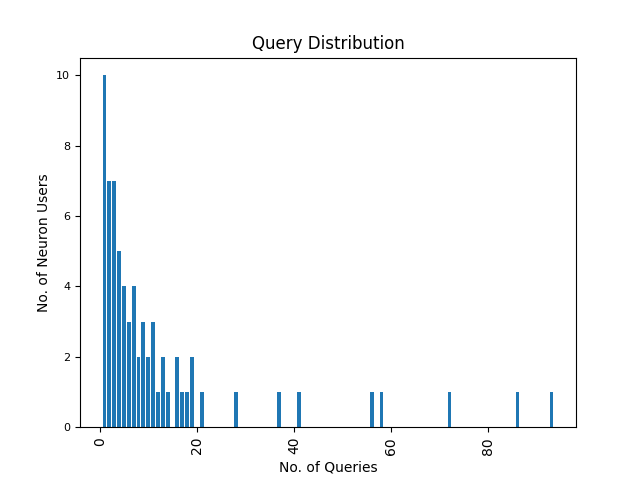
\includegraphics[width=0.7\linewidth]{neuron-no-query.png}
\vspace{0ex}\caption{No. of queries versus no. of users.}
\label{fig:query}
%\hrule
\vspace{0ex}\end{figure}

We observe the usage of \textsc{neuron} from 14th October to 2nd December by analyzing the log file. Note that 12th November was the last date of the course culminating with the submission of a course project. Since a user needs to access \textsc{neuron} by logging using an email address, we were able to match majority of the email addresses that accessed it with those registered for the course. There were 69 distinct learners (41.5\%) using \textsc{neuron} during this period. Figure~\ref{fig:neuron}(b) reports the number of queries posed by learners over time. In total, 888 valid \textsc{sql} queries (484 distinct queries) were executed on \textsc{neuron}. The distribution of the number of queries versus the number of distinct learners who posed that number of queries is shown in Figure~\ref{fig:query}. Observe that more than 85\% of them posed more than one query and the maximum number of queries posed by a single user is 93! Prior to October 28th (test date), the number of distinct users is 48 and the number of queries posed is 409 (211 distinct queries). Hence, the usage of \textsc{neuron} continued even after the test as learners may be using it to understand \textsc{qep}s for their project work. Some students used it even after the official end date of the course probably demonstrating intrinsic motivation to explore \textsc{qep}s. 

To investigate whether \textsc{neuron} may benefit learners to understand \textsc{qep}, we use the test as a proxy. In the test, a question was specifically set to this end. The students were asked to explain in natural language the visual format of a \textsc{qep}  (in PostgreSQL) for an \textsc{SQL} query on IMDb database involving two joins, scans, and sort operations. The question carried 10 marks. Observe that it matches very closely to \textsc{neuron}'s goal. This enables us to evaluate more accurately possible impact of \textsc{neuron} on the test performance.  

 In order to avoid any bias, a teaching assistant (TA) who is not involved with \textsc{neuron} graded the answers to this question.  The TA was given the solution and was allowed to set the marking scheme for the question. The number of students who took the test is 162. The average score of students who used (resp. not used) \textsc{neuron} prior to test is 8.43 (resp. 7.07). The maximum, minimum, and median scores of these two groups are (10, 6.5, 8) and (10, 0, 7.5), respectively. Among the non-\textsc{neuron} users, the percentage of students with scores lower than the minimum score in the \textsc{neuron} user group (\ie 6.5)  is 21.31\%.  Furthermore, the percentage of \textsc{neuron} users (resp. non-\textsc{neuron} users) with scores higher than the average score of 8 is 47.5\% (resp. 35.25\%). Some of the common errors made by students are (a) not describing in natural language; (b) incorrect sequence of steps; (c) not including filter conditions in the scan operations; and (d) unclear specifications of operators and intermediate results. Observe that these errors could have been mitigated with the usage of \textsc{neuron}.

 In summary, while we cannot infer causal link from the initial results, it is possible \textsc{neuron} may improve learning of query execution strategies. We are still in the early stages of understanding the impact of this tool on learning. We intend to use \textsc{neuron} and \textsc{lantern} in future semesters to gather sufficient longitudinal data for a more detailed investigation of technology-enabled learning and their impact on data-driven education.

%====================================================================================================
\section{Conclusions}
\label{concl}
%====================================================================================================
Impact of digital technologies on learning has consistently shown positive benefits when they are aligned.  With the advent of data science and lifelong learning, there has been growing interest in the database course from adult learners with diverse background. This necessitates us to revisit the traditional way we teach this course by supplementing it with technological support to improve learning. This paper contributes a vision of technology-enabled learning of the topic of relational query processing in a database systems course. Specifically, our vision attempts to carve out a substantially new research topic that is at the intersection of learning sciences and data management to improve learning of relational query processing.  To the best of our knowledge, this vision has not been systematically investigated before, prior to our recent publications.

\vspace{1ex}\noindent\textbf{Measures of success.} Successful realisation of this vision will improve learning and understanding of the complex topic of relational query processing. But several non-trivial and novel research challenges as articulated in the paper need to be overcome to realize  it. Adoption of the potential solutions by real-world learners as a supplement to traditional modes of learning will be another measure of success.

\vspace{1ex}\noindent\textbf{Wider applicability.} We focused on the topic of relational query processing since it is one of the most challenging topic in a database systems course. Nevertheless, it is easy to see that our vision of technology-enabled learning can be extended to other topics such as enabling technologies to facilitate learning of \textsc{sql} queries.


\begin{thebibliography}{10}
	\itemsep=1pt
	\begin{small}
	
	\bibitem{imdb} The IMDb database. \url{https://relational.fit.cvut.cz/dataset/IMDb}.
	
	\bibitem{msdn} Advanced query tuning concepts. \url{https://docs.microsoft.com/en-us/previous-versions/sql/sql-server-2008-r2/ms191426(v=sql.105)?redirectedfrom=MSDN}, 2012.
	
	\bibitem{lantern-soft} \textsc{lantern} software. \url{https://howardlee.cn/lantern/}.
	
	\bibitem{mocha-soft} \textsc{mocha} software. \url{https://howardlee.cn/mocha/}.
	
	\bibitem{neuron-soft} \textsc{neuron} software. \url{https://howardlee.cn/#/}.

\bibitem{unesco} USESCO Insititute of Lifelong Learning. UNESCO Global Network of Learning Cities. Accessible at \url{https://uil.unesco.org/lifelong-learning/learning-cities}, 2019.

\bibitem{AP12} E. M. Anderman, H. Patrick. Achievement goal theory, conceptualization of ability/intelligence, and classroom climate. \textit{In Handbook of research on student engagement},  Springer: Boston, MA, 2012.

\bibitem{BC+15} A. Bhangdiya, B. Chandra, B. Kar, B. Radhakrishnan, K. V. M. Reddy, S. Shah, S. Sudarshan.
The XDa-TA system for automated grading of SQL query assignments. \textit{In ICDE}, 2015.

\bibitem{BB11} E. L. Bjork, R. Bjork.  Making things hard on yourself, but in a good way. \textit{Psychology in the Real World}, 59-68, 2011.

\bibitem{BDK13} R. A. Bjork, J. Dunlosky, N. Kornell. Self-regulated learning: Beliefs, techniques, and illusions. \textit{Annual review of psychology}, 64, 417–444, 2013.

\bibitem{borovicaGajic2018} R. Borovica-Gajic, S. Idreos, A. Ailamaki, M. Zukowski, C. Fraser. Smooth scan: robust access path selection without cardinality estimation. \textit{The VLDB Journal}, 27(4):521-545, 2018.

\eat{\bibitem{BCR09} N. Bruno, S. Chaudhuri, R. Ramamurthy. Interactive plan hints for query optimization.\textit{ In SIGMOD}, 2009.}

\bibitem{CP79} J. T. Cacioppo and R. E. Petty. Effects of Message Repetition and Position on Cognitive Response, Recall, and Persuasion. \textit{Journal of Personality and Social Psychology} ,37, 1: 97-109, 1979.

\bibitem{SC98} S. Chaudhuri. An Overview of Query Optimization in Relational Systems. \textit{In PODS}, 1998.

\bibitem{lantern-demo} P. Chen, H. Li, S. S. Bhowmick, S. R. Joty, W. Wang. LANTERN: Boredom-conscious Natural Language Description Generation of Query Execution Plans for Database Education.\textit{ In SIGMOD}, 2022.

\bibitem{DG11} J. Danaparamita, W. Gatterbauer. QueryViz: Helping Users Understand SQL Queries and Their Patterns. \textit{In EDBT}, 2011.

\bibitem{DV+91} E. L. Deci, R. J. Vallerand, L. G. Pelletier, R. M. Ryan. Motivation and education: The self-determination perspective. Educational psychologist, 26(3-4), 325-346, 1991.

\bibitem{dbtext} H. Garcia-Molina, J. D. Ullman, J. Widom. Database Systems: The Complete Book. \textit{Prentice-Hall}, 2002.

\bibitem{GK12} M. Gawade, M. L. Kersten. Stethoscope: A platform for interactive visual analysis of query execution plans . \textit{PVLDB}, 5(12), 2012.

\bibitem{Gross} R. Gross. Psychology: The Science of Mind and Behaviour. \textit{Hachette UK}, ISBN 978-1-4441-6436-7.

\bibitem{GGL18} J. Gao, M. Galley, L. Li. Neural Approaches to Conversational AI. \textit{In ACL}, 2018.

\bibitem{picasso} J. R. Haritsa.  The Picasso Database Query Optimizer Visualizer. \textit{In PVLDB}, 3(2), 2010.

\bibitem{HK13} M. R. Hastall and S. Knobloch-Westerwick. Severity, Efficacy, and Evidence Type as Determinants of Health Message Exposure. \textit{Health Communication}, 28, 4: 378-388, 2013.

\bibitem{HG+11} G. Hervet, K. Guerard, S. Tremblay, M. Saber Chtourou. Is Banner Blindness Genuine? Eye Tracking Internet Text
Advertising. \textit{Applied Cognitive Psychology}, 25, 5: 708-716, 2011.

\bibitem{HXK12} S. Higgins, Z. M. Xiao, M. Katsipatak. The Impact of Digital Technology on Learning: A Summary for the Education. \textit{Education Endowment Foundation}, 2012.

\bibitem{HM+22} Y. Hu, Z. Miao, Z. Leong, H. Lim, Z. Zheng, S. Roy, K. Stephens-Martinez, J. Yang. I-Rex: An Interactive Relational Query Debugger for SQL. \textit{In ACM Technical Symposium on Computer Science Education (SIGCSE)}, 2022.

\bibitem{panel} Z. Ives,  J. Gehrke, J. Giceva, A. Kumar, R. Pottinger. VLDB Panel Summary: "The Future of Data(base) Education: Is the Cow Book Dead?". \textit{SIGMOD Rec.}, 50(3), 2021.

\bibitem{kazdin} A. E. Kazdin. Motivation: an overview. \textit{Encyclopedia of Psychology}, American Psychological Association,  ISBN 978-1-55798-187-5, 2000.

\bibitem{KS+20} H. Kim,  B.-H. So, W.-S. Han, H. Lee. Natural Language to SQL: Where Are We Today? \textit{PVLDB}, 13(10), 2020.

\bibitem{KV+12} A. Kokkalis, P. Vagenas, A. Zervakis, A. Simitsis, G. Koutrika, Y. E. Ioannidis. Logos: A System for Translating Queries into Narratives. \textit{In SIGMOD}, 2012.

\bibitem{LZ+20} A. Leventidis, J. Zhang, C. Dunne, W. Gatterbauer, H. V. Jagadish, M. Riedewald. QueryVis: Logic-based Diagrams help Users Understand Complicated SQL Queries Faster. \textit{In SIGMOD}, 2020.

\bibitem{neuron} S. Liu, S. S. Bhowmick, W. Zhang, S. Wang, W. Huang, S. Joty. NEURON: Query Optimization Meets Natural Language Processing For Augmenting Database Education. \textit{In SIGMOD}, 2019.

\bibitem{MRY19} Z. Miao, S. Roy, J. Yang. Explaining Wrong Queries Using Small Examples. \textit{In SIGMOD}, 2019.

\bibitem{MF21} D. Miedema, G. Fletcher. SQLVis: Visual Query Representations for Supporting SQL Learners. \textit{In VL/HCC}, 2021.


\bibitem{MAF21} D. Miedema, E. Aivaloglou, G. Fletcher. Identifying SQL Misconceptions of Novices: Findings from a Think-Aloud Study. \textit{In ICER}, 2021.

\bibitem{NL09} J. Nakamura, M. Csikszentmihalyi. Flow theory and research. \textit{Oxford Handbook of Positive Psychology}, Oxford University Press, 2009.

\bibitem{cow} R. Ramakrishna, J. Gehrke.  Database Management Systems. \textit{McGraw-Hill, Inc.}, USA, 2020.


\bibitem{RD00} R. M. Ryan, E. L. Deci. Intrinsic and extrinsic motivations: Classic definitions and new directions. \textit{Contemporary educational psychology}, 25(1), 54-67, 2000.

\bibitem{SPC90} D. W. Schumann, R. E. Petty, D. S. Clemons. Predicting the Effectiveness of Different Strategies of Advertising Variation: A Test of the Repetition-Variation Hypotheses. \textit{Journal of Consumer Research}, 17, 2: 192, 1990.

\bibitem{SB15} N. C. Soderstrom, R. A. Bjork.  Learning versus performance: An integrative review. \textit{Perspectives on Psychological Science}, 10(2), 176-199, 2015.

\bibitem{mocha} J. Tan,  D. Yeo, R. Neoh, H.-E. Chua, S. S. Bhowmick. MOCHA: A Tool for Visualizing Impact of Operator Choices in Query Execution Plans for Database Education.  \textit{PVLDB}, 15(12), 2022.

\bibitem{TR10} K. Taylor, D. Rohrer. The effects of interleaved practice. \textit{Applied Cognitive Psychology}, 24(6), 2010.

\bibitem{lantern} W. Wang, S. S. Bhowmick, H. Li, S. Joty, S. Liu, P. Chen. Towards Enhancing Database Education: Natural Language Generation Meets Query Execution Plans.\textit{ In SIGMOD}, 2021.


\bibitem{WE00} A. Wigfield, J. S. Eccles. Expectancy-value theory of achievement motivation. \textit{Contemporary educational psychology}, 25(1), 68-81, 2000.

\bibitem{ZJ+22} C. Zhu, C. Ji, Y. Zhang, X. Liu, A. Jatowt, S. S. Bhowmick, C. Sun, T. Zhao. Towards Automatic Support for Leading Court Debates: A Novel Task Proposal \& Effective Approach of Judicial Question Generation.  {\em To Appear in Neural Computing and Applications (NCAA)\/}, Springer, 2022.
	
	\end{small}
\end{thebibliography}


\end{document}
\end{article}

\begin{article}
{Principles of Query Visualization}
{Wolfgang Gatterbauer, Cody Dunne, H.V.\ Jagadish, and Mirek Riedewald}
\documentclass[letterpaper,11pt]{article}
\usepackage{deauthor}
\usepackage{times}
\usepackage{graphicx} 
\usepackage{amssymb}	%
\usepackage{amsmath}

\usepackage{xcolor,colortbl}    %
%
%
%
%
%
%
%

%
%
%
%
%




\usepackage{xspace}            %

\newcommand{\queryvis}{\textsf{QueryVis}\xspace}
\newcommand{\diagrams}{\textsf{Relational Diagrams}\xspace}

\newcommand{\sql}[1]{\textup{\textsf{\small#1}}}



%
%
\usepackage{scalerel}
\usepackage{tikz}

\usetikzlibrary{svg.path}

\definecolor{orcidlogocol}{HTML}{A6CE39}
\tikzset{
  orcidlogo/.pic={
    \fill[orcidlogocol] svg{M256,128c0,70.7-57.3,128-128,128C57.3,256,0,198.7,0,128C0,57.3,57.3,0,128,0C198.7,0,256,57.3,256,128z};
    \fill[white] svg{M86.3,186.2H70.9V79.1h15.4v48.4V186.2z}
                 svg{M108.9,79.1h41.6c39.6,0,57,28.3,57,53.6c0,27.5-21.5,53.6-56.8,53.6h-41.8V79.1z M124.3,172.4h24.5c34.9,0,42.9-26.5,42.9-39.7c0-21.5-13.7-39.7-43.7-39.7h-23.7V172.4z}
                 svg{M88.7,56.8c0,5.5-4.5,10.1-10.1,10.1c-5.6,0-10.1-4.6-10.1-10.1c0-5.6,4.5-10.1,10.1-10.1C84.2,46.7,88.7,51.3,88.7,56.8z};
  }
}

\DeclareRobustCommand{\orcidiconlink}[2]{%
    \hypersetup{urlcolor=black}%
    \href{https://orcid.org/#2}{#1 \mbox{\scalerel*{%
        \begin{tikzpicture}[yscale=-1,transform shape]%
            \pic{orcidlogo};%
        \end{tikzpicture}%
    }{|}}}%
}%
%
%



%\usepackage[caption=false]{subfig} 
\usepackage{subfig}

\newcommand{\smallsection}[1]{\vspace{5mm}\noindent\textbf{#1.}}	%
\newcommand{\introparagraph}[1]{\textbf{#1.}}        %






%
%

\newtoks\bsubfloattoks
\newdimen\bsubfloatht

\makeatletter
\newenvironment{bsubfloatrows}[1][\quad]
  {\def\bsubfloatspace{#1}\resetbsubfloatrows
   \def\\{\printbsubfloatrow\resetbsubfloatrows\par
     \@ifnextchar[{\bsubfloatvspace}{}}%
   \def\bsubfloatvspace[##1]{\vspace{##1}}%
  }
  {\printbsubfloatrow}
\newcommand{\bsubfloat}[2][]{%
  \sbox\z@{#2}%
  \ifdim\bsubfloatht<\ht\z@
    \bsubfloatht=\ht\z@
  \fi
  \bsubfloattoks=\expandafter{\the\bsubfloattoks
    \bsubfloatspace\subfloat[#1]{\vbox to\bsubfloatht{\hbox{#2}\vfill}}}%
}
\newcommand\resetbsubfloatrows{\bsubfloatht\z@\bsubfloattoks={\@gobble}}
\newcommand{\printbsubfloatrow}{\the\bsubfloattoks}
\makeatother
%



%
%
%
%
\renewcommand\topfraction{1}
\renewcommand\bottomfraction{1}
\renewcommand\textfraction{0}            %
\renewcommand\floatpagefraction{1}
\renewcommand\dbltopfraction{1}
\renewcommand\dblfloatpagefraction{1}
\setcounter{totalnumber}{50} %
\setcounter{topnumber}{50} %
\setcounter{dbltopnumber}{50} %
\setcounter{bottomnumber}{50}


\usepackage{url}
\urlstyle{rm}

		

%
%
%
%
%
%\newtheorem{theorem}{Theorem}  	%
\newtheorem{scenario}{Scenario}              	
%\newtheorem{definition}{Definition}    %



%\usepackage[colorlinks, allcolors=blue]{hyperref}
\usepackage{hyperref}

\def\scenarioautorefname{Scenario}%
\def\subfigureautorefname{Figure}%
\def\subsectionautorefname{Section}%




\newcommand{\osfpreprintplain}{osf.io/btszh}
\newcommand{\osfsupplementplain}{osf.io/mycr2}
\newcommand{\osfpreregplain}{osf.io/mycr2}
\newcommand{\osfpreprint}{\formattedurl{https://\osfpreprintplain}{\osfpreprintplain}}
\newcommand{\osfpreprintlong}{\formattedurl{https://\osfpreprintplain}{https://\osfpreprintplain}}
\newcommand{\osfsupplement}{\formattedurl{https://\osfsupplementplain}{\osfsupplementplain}}
\newcommand{\osfsupplementlong}{\formattedurl{https://\osfsupplementplain}{https://\osfsupplementplain}}
%
\newcommand{\osfprereg}{\url{https://\osfpreregplain}}
\newcommand{\formattedurl}[2]{\href{#1}{\small\texttt{#2}}\xspace}



\graphicspath{{submissions/query-vis-gatterbauer/}}


\begin{document}

\title{Principles of Query Visualization}

\author{
  \hspace{-15mm}\phantom{x}
  \texorpdfstring{\orcidiconlink{Wolfgang Gatterbauer}{0000-0002-9614-0504}}{Wolfgang Gatterbauer}
  \hspace{-15mm}\phantom{x}  
  \\
  \hspace{-6mm}\phantom{x}
  Northeastern University
  \hspace{-6mm}\phantom{x}
  \\
  \footnotesize
  \hspace{-15mm}\phantom{x}
  w.gatterbauer@northeastern.edu
  \hspace{-15mm}\phantom{x}  
\and
  \texorpdfstring{\orcidiconlink{Cody Dunne}{0000-0002-1609-9776}}{Cody Dunne}\\
  \hspace{-6mm}\phantom{x}
  Northeastern University
  \hspace{-6mm}\phantom{x}
  \\
  \footnotesize
  \hspace{-15mm}\phantom{x}
  c.dunne@northeastern.edu
  \hspace{-15mm}\phantom{x}  
\and
  \texorpdfstring{\orcidiconlink{H.V.\ Jagadish}{0000-0003-0724-5214}}{H.V.\ Jagadish}\\
  \hspace{-6mm}\phantom{x}
  University of Michigan
  \hspace{-6mm}\phantom{x}
  \\
  \footnotesize
  jag@umich.edu
\and
  \hspace{-15mm}\phantom{x}
  \texorpdfstring{\orcidiconlink{Mirek Riedewald}{0000-0002-6102-7472}}{Mirek Riedewald}
  \hspace{-15mm}\phantom{x}  
  \\
  \hspace{-6mm}\phantom{x}  
  Northeastern University
  \hspace{-6mm}\phantom{x}
  \\
  \footnotesize
  \hspace{-15mm}\phantom{x}  
  m.riedewald@northeastern.edu  
  \hspace{-15mm}\phantom{x}  
}

\maketitle





\begin{abstract}
Query Visualization (QV) is the problem of transforming a given query into a graphical representation
that helps humans understand its meaning.
This task is notably different from designing a Visual Query Language (VQL)
that helps a user compose a query.
This article discusses 
the principles of relational query visualization
and its potential for simplifying user interactions with relational data.



\end{abstract}





\section{What is Query Visualization (QV) and what is it for?} 
\label{sec:1}



%
%
%
%
%
%
%

The design of relational query languages and the difficulty for users to compose relational queries have
received much attention over the 
last 40 years~\cite{DBLP:journals/vlc/CatarciCLB97, 
ChanUserDatabaseInterface:1993,
GREENE1990303,
Harel:Nonprocedural:1985,
FrameworkForChoosingQueryLanguages:1985,
LEGGETT1984493,
DBLP:journals/csur/Reisner81, 
Reisner1975:HumanFactors,
Welty-Stemple:1981,
scamell:1993}.
A complementary and much-less-studied problem is that of helping users 
\emph{read and understand an existing query}.  
Reading code is hard, and SQL is no exception.  
With the proliferation of public data sources, and associated queries, users increasingly have a need to read other people's queries and scripts.  
Furthermore, it is usually much easier to modify a draft than to write something from scratch.  
As such, modifying an already existing query could be an effective way to write new queries.
However, modifying an existing query requires first to understand it (\autoref{Fig_TheVision}). 
For these reasons, it is valuable to help users understand queries,
and visualization is one obvious route.
In this paper, we study the problem of query visualization with a view towards improving query understanding.


Consider the following five scenarios that illustrate how query visualizations can assist users:




\begin{scenario}[Data scientists reusing past queries]\label{scenario:1}
	A group of data analysts 
	are collaboratively analyzing movie data.
	This data is stored in a shared data repository. 
	In addition to the data itself, they are also sharing their queries using a Collaborative Query Management System (CQMS)
	\cite{QueRIERecommendations:2010,
	ARZAMASOVA2021101646,
	DBLP:conf/ssdbm/ChatzopoulouEP09,
	Eirinaki:QueRie:2014,
	DBLP:conf/icde/FanLZ11,
	HoweC2010:SQLshare, SQLshare:2016,
	DBLP:conf/cidr/KhoussainovaBGKS09, KhoussainovaKBS:2011, LiFWWF2011:DBease,
	Marcel:QueryRecommendations:2011,
	Milo:REACT:2016}.	
	The query recommendation component of that tool suggests relevant previously-issued queries that the user can choose from, 
	rather than write a query from scratch.
	The tool shows the queries both in text (\autoref{Fig_KevinBacon_a})
	and as query visualization (\autoref{Fig_KevinBacon_b}).
	The visualization preserves the logical structure of the textual query.
	 %
	 There is also a one-to-one mapping between the query and its visualization:
	%
	As the user moves the mouse over components of the visualization, the corresponding component in the textual query is highlighted (and v.v.).
	The particular query used in 
	\autoref{Fig_KevinBacon}
	is over the IMDB movie database and finds all actors with Kevin Bacon number 2
	(i.e.\
	actors who have not played in a movie with Kevin Bacon directly, 
	but who have played with other actors who have played with Kevin Bacon).\footnote{See \url{https://youtu.be/kVFnQRGAQls?t=170} for an animated explanation of how to read and understand  this particular query.}
	%
%
	These diagrams require some training to understand (see our discussion in \autoref{sec:2} for how to read them). 
	However, in a controlled and pre-registered user study  (see \autoref{sec:userstudy})
	we found that even a few minutes of training
	suffice, and experienced SQL users could interpret queries \emph{in less time} and \emph{with fewer errors} 
	using these diagrams instead of using SQL alone \cite{DBLP:conf/sigmod/LeventidisZDGJR20}.




	A widely known example of such a shared data and query repository is the Sloan Digital Sky Survey (SDSS)~\cite{QueRIERecommendations:2010, SDSS}.
	Data about stars was put into a relational database and is freely available for access. 
	%
	Astronomers, who are mostly ``hobbyist" SQL users, 
	have to write queries to get the data they want.
	In most cases, the queries they wish to write are similar to queries others have written before.  So the standard workflow is for the user 
	%
	to look at previously issued queries, find one that is close to what they want, and then modify it to suit their analysis needs.
	In response, SDSS has added templates for commonly written query types.\footnote{\url{http://skyserver.sdss.org/dr8/en/help/docs/realquery.asp}} 
	
		%
	%


	%
	%
	%
	%
	%
\end{scenario}

	%
	%
	%


	%
	%




\begin{figure}[t]
%
   \centering
\subfloat[SQL query]{
	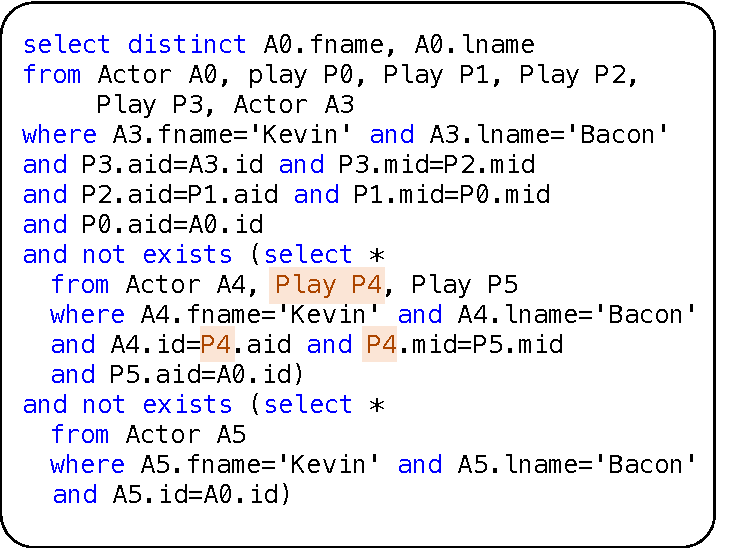
\includegraphics[scale=0.58]{figs/Fig_KevinBaconNew_a}
	\label{Fig_KevinBacon_a}}
\hspace{4mm}
\subfloat[Query Visualization]{
	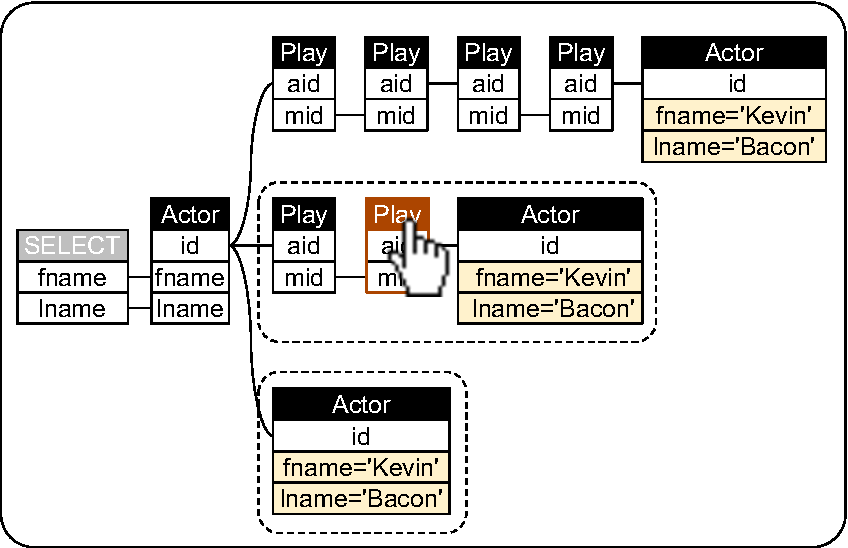
\includegraphics[scale=0.58]{figs/Fig_KevinBaconNew_b}
	\label{Fig_KevinBacon_b}}	
%
	\caption{\autoref{scenario:1}: A user searches for a query by browsing through a repository 
	of previously-recorded SQL queries.
	For each query, she needs to \emph{quickly understand} its meaning. 
	A query visualization panel helps her understand the query by showing a 
	succinct representation of its relational query pattern. 
	The shown query returns actors with Bacon number 2.
	As she hovers her mouse over parts of the query, 
	both the textual and visualized query highlight corresponding parts in synchronization.
		%
		%
	%
}
\label{Fig_KevinBacon}
\end{figure}



\begin{scenario}[Visual feedback during query editing]
	As the user starts editing the SQL query (\autoref{Fig_KevinBacon_a}), the query visualization gets updated too
	(\autoref{Fig_KevinBacon_b}, updates are not shown).
	When a syntactically-correct query does not give the expected result,
	the query visualization can help the user understand that an incorrect join pattern was used between the various subqueries. 
		%
		%
\end{scenario}	








\begin{scenario}[Learning from galleries of relational query patterns]
	A data scientist wants to issue another query and looks for inspiration in a \emph{web gallery of SQL design patterns}.
	Similar to the way users of Matplotlib\footnote{\url{https://matplotlib.org/stable/gallery/index.html}},
	 D3\footnote{\url{https://d3-graph-gallery.com/}}, 
	and Altair\footnote{\url{https://altair-viz.github.io/gallery/index.html}} 
	%
	program new visualizations by browsing through, copying from, and adapting existing designs~\cite{10.1145/3503490}, 
	such galleries enhance the technical skills of data scientists and learners by 
	showing a range of possible relational patterns and design templates to learn from 
	that would be hard to browse and make sense of 
	based on text alone.
	Similar programmer behaviors are found outside of visualization, where existing code templates, examples, and idioms are extensively copied and adapted.
	%
	From IDE (Integrated Development Environment) logs of 81 developers, 
	Ciborowska et al.\ \cite{Ciborowska2018} identified many cases of opportunistic code reuse from the Web
	followed by editing the code. 
	%
	%
	LaToza et al.~\cite{Latoza2006} surveyed 157 programmers, 
	%
	and 56\% agreed that understanding code that someone else wrote is a serious problem.
	Yang et al.~\cite{Yang2017} found that many blocks of Python code are copied from Stack Overflow 
	into open-source projects with slight modifications. 
	Ahmed et al.~\cite{Ahmed2015} found that 24\%
	of copy-and-paste events 
	%
	%
	among 21,770 users of Eclipse were from sources external to the IDE, though this is likely an overestimate. 
	Brandt et al.~\cite{Brandt2009} found that such copy-and-paste programming is particularly beneficial for programmers working in new domains:
	In their study of students learning to use a new framework, one-third of the participants' code consisted of modified versions of examples from the documentation. 
	%
	%

	
	
	%
	
%
		%
		%
		%
		%
		%


		%
        %
        %
        %
        %
        %
        %
        %
        %
        %
        %
        %
        %
        %
        %
        %
        %
        %
        %
        %
        %
        %
        %
        %
        %
        %
        %
        %
        %
        %
        %
        %
        %
        %
        %
        %
	%
	%
	
		%
		%
		%
		%
\end{scenario}	


\begin{scenario}[Clustering pattern-identical queries]
	A teacher receives the SQL solutions for a homework from her 50 students. 
	An automatic correction tool, such as
	ADUSA~\cite{DBLP:conf/kbse/KhalekELK08},
	Cosette~\cite{DBLP:conf/cidr/ChuWWC17},
	Qex~\cite{DBLP:conf/lpar/VeanesTH10}
	TATest~\cite{MRJ:ExplainingWrongQueries:2019},
	or XData~\cite{DBLP:journals/vldb/ChandraCKRS015},
	%
	%
	determines that 40 of those solutions are correct. But those correct solutions ``look'' very different,
	even after applying some standard SQL pretty printer,
	such as sqlparse~\cite{sqlparse}.
	%
	%
	%
	%
	%
	%
	%
	The queries use different table aliases, nesting patterns, join sequences, and at times different syntactic constructs, 
	such as
	implicit joins in the WHERE clause
	or infixed SQL-92 join notation.
	%
	%
	%
	%
	%
	%
	%
	%
	%
	%
	%
	%
	%
	%
	The teacher would like to cluster the 40 correct solutions not by their syntactic variants, but 
	%
	by whether there
	%
	are `truly' 
	\emph{novel patterns} beyond the 3 she currently knows.
		%
		%
		%
		%
		%
		%
		%
		%
		%
	Query visualization makes it easier to cluster and compare the 40 queries, because a good visualization
	captures the essence of the query structure, abstracting away superficial
	syntactic differences.	
	And, indeed, the teacher finds 2 new patterns.
	She can now show and discuss 5 total patterns with the learners in the next class.
\end{scenario}	





\begin{scenario}[Visual feedback from voice assistants]
	\label{scenario:5}
	We now switch to the year 2045.
	%
	A data analyst 
	stands in her office analyzing some company data. 
	She directs possible queries to her voice assistant 
	which then visualizes on the walls the queries 
	together with the data (\autoref{Fig_SpeechAssistant}). 
	The visualization of the query provides immediate feedback on what the assistant understood.
\end{scenario}



	%
	%
	%
	%
	%
	%


\begin{figure}
    \centering
    \begin{minipage}{0.5\textwidth}
        \centering
        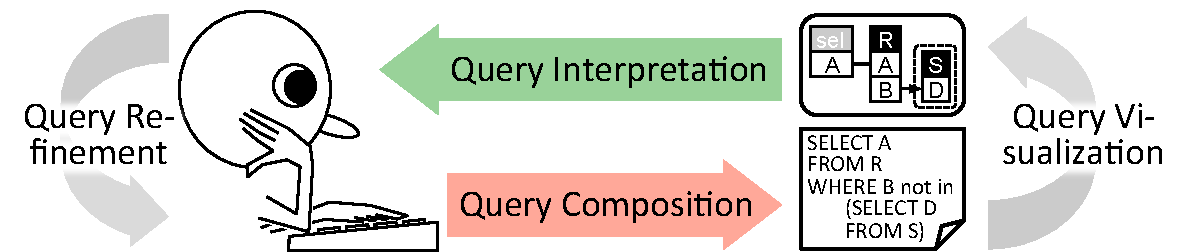
\includegraphics[scale=0.425]{figs/Fig_TheVision}
		\caption{The goal of query visualization is to complement (but not substitute) the composition of queries 
		by creating automatic visualizations of queries. 
		Composition of a query is still performed via unambiguous and expressive text. 
		The transformation from text into a visualization can abstract away from a concrete syntax and thus be non-injective. 
		Compare to the write-format-preview cycle used by LaTeX~\cite{latex} in that a user writes text, 
		the system then autoformats and renders a document, 
		which the user can then peview.
		%
		%
		%
		}
		\label{Fig_TheVision}
    \end{minipage}
	\hfill
    \begin{minipage}{0.45\textwidth}
        \centering
        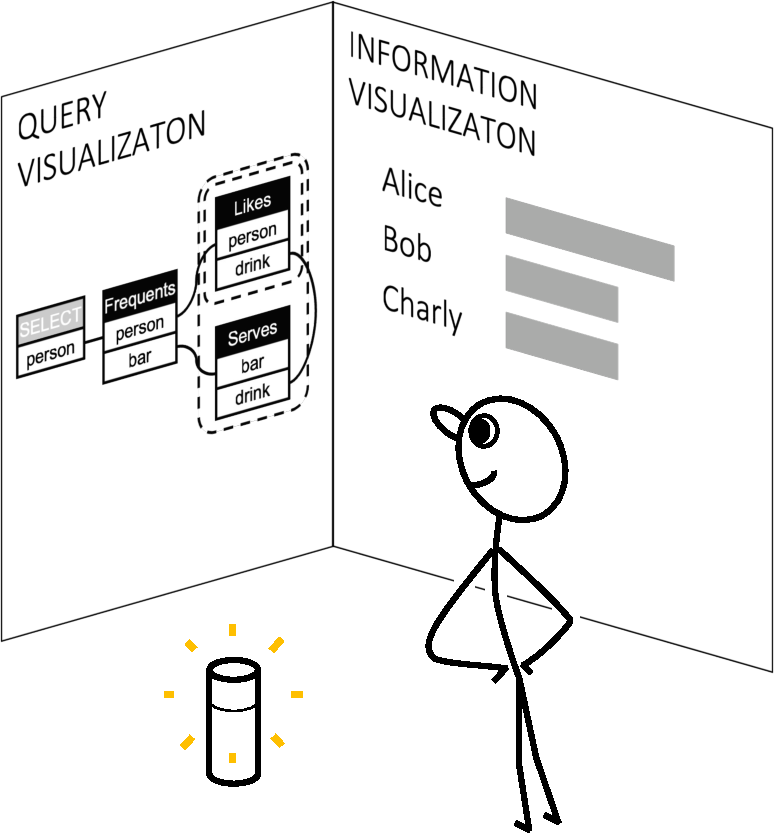
\includegraphics[scale=0.36]{figs/Fig_SpeechAssistantv2}
		\caption{\autoref{scenario:5}: An analyst dictates queries to her voice assistant which then shows the query as understood 
		together with the query answers.}
		\label{Fig_SpeechAssistant}
    \end{minipage}
\end{figure}


	%
	%
	%
	%
	%
	%
	%
	%
	%
	%
	%
	%
	%
	%
	%
	%
	%
	%
	%
	%
	%
	%




Common to these 5 scenarios is that query visualization helps the users achieve new functionalities 
or increased efficiency in composing queries
as a \emph{complement} to query composition and 
\emph{not a substitute} for it.
%
	%
	%
	%
%
%
	%
	%
	%
	%


\begin{definition}[Query Visualization]
The term ``query visualization'' refers to both ($i$) a graphical representation of a query 
and ($ii$) the process of transforming a given query into a graphical representation.
The goal of query visualization is to help users more quickly understand the intent of a query,
as well as its relational query pattern.
\end{definition}

When we say ``query visualization", we will typically mean the end result. 
From context, it should be clear to the reader on the few occasions when we mean the process rather than the end result.

	%
	%
	%
	%
	%
	%
	%
	%
	%
	%
	%
	%
	%
	%
	%
	%
	%
	%
	%
	%
	%

	%
	%
	%
	%
	%
	%
	%











\section{What Query Visualization is not}
\label{section:whatisQVnot}


\subsection{Query Visualization is not the same as a Visual Query Language (VQL)}
\label{QVisnotVQL}

Visual Query Languages (VQLs) provide languages to express queries in a visual format.
Visual Query Systems (VQSs) implement VQLs and generate queries from visual representations constructed by users~\cite{DBLP:reference/db/Catarci18a}.
Such visual methods for specifying relational queries have been studied
extensively
(a 1997 survey by Catarci et al.~\cite{DBLP:journals/vlc/CatarciCLB97} 
cites over 150 references), and
many commercial database products offer some visual interface for users to write SQL queries.  
In parallel, there is a centuries-old history on the study of formal diagrammatic reasoning systems \cite{DBLP:conf/iccs/Howse08}
with the goal of helping humans to reason in terms of logical statements.\footnote{A relational query is a logical formula with free variables. 
A logical statement has no free variables and is intuitively the same as a Boolean query that returns a truth value of TRUE or FALSE. }
Yet despite their extensive study and intuitive appeal, successful visual tools today mostly only 
\emph{complement instead of 
replace}
%
text for specifying queries.
Why has visual query specification not yet replaced textual query specification?




\begin{figure}[t]
\centering
\begin{minipage}{0.50\textwidth}
	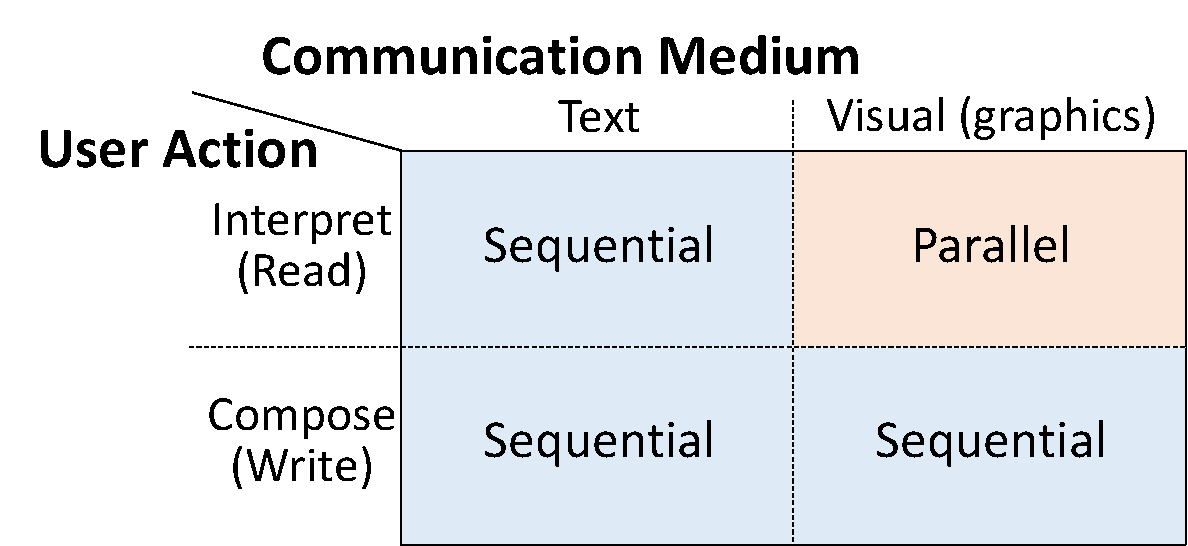
\includegraphics[scale=0.35]{figs/Fig_MatrixDataQueryNew}
	\caption{%
	    \emph{Composing} a query with a visual query language is as sequential as composing it with SQL. 
        \emph{Interpreting} a visualization (whether of information or a query) 
		is the only modus in which a user can act on information in parallel, 
		leveraging the speed of the human perceptual system 
		(orange = easier, blue = harder).
    }
    \label{Fig_MatrixDataQueryNew}
\end{minipage}
\hfill
\begin{minipage}{0.45\textwidth}
	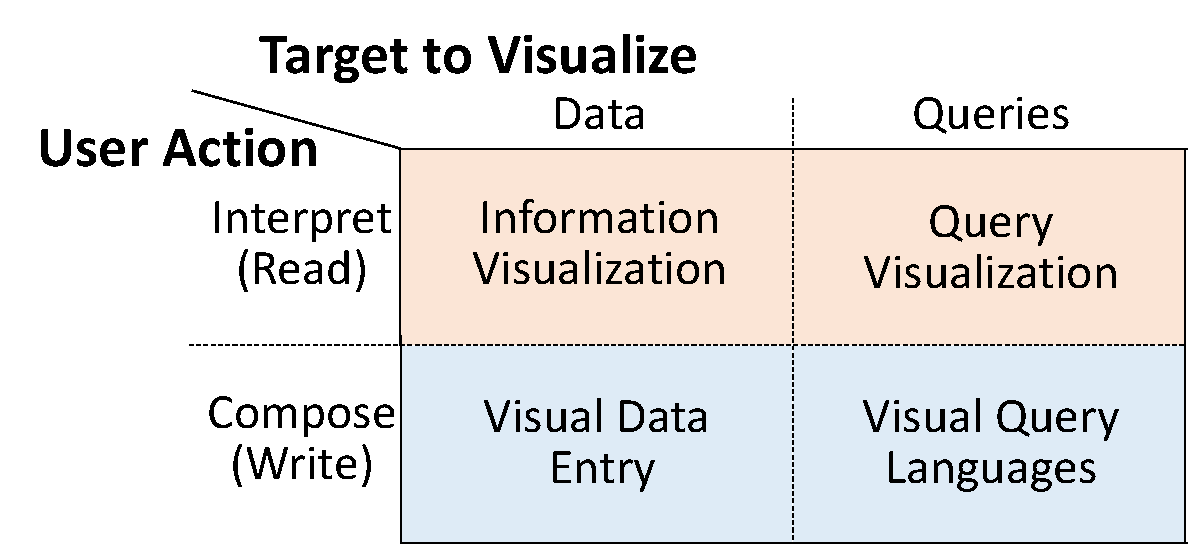
\includegraphics[scale=0.35]{figs/Fig_MatrixTextGraphicsNew}
	\caption{%
	    \emph{Visual Query Languages} allow a user to compose queries. 
		They have been widely studied and have a rich history.
	    In contrast, \emph{Query Visualization} helps the user understand an existing query 
		just as \emph{Information Visualization} helps understand data 
		(orange = easier, blue = harder).
    }
	\label{Fig_MatrixTextGraphics}
\end{minipage}
\end{figure}




We believe that there are two primary reasons:
(1) First, humans are \emph{better in interpreting rather than composing visuals} because visual composition is an inherently sequential process (\autoref{Fig_MatrixDataQueryNew}).
All human input methods (composition) are sequential, whether resulting in text or a graphic. Visual perception is a remarkable human sense (interpretation) that can 
understand inputs
in parallel,
%
and it works dominantly by \emph{spatial arrangement of information}. 
While reading text is also a visual activity, the spatial arrangement of the letters requires a sequential scan of the text 
(though notice that pretty printers can spatially arrange text, \autoref{section:alternatives}).
Hence, visual interpretation of graphics is the fastest way to communicate with humans, 
and it only works well for understanding rather than composing.
Even in theory, there is no dramatic speed-up 
%
in
using a visual language for composition. 
In practice, the user interaction is quite cumbersome: 
users must be able to interactively construct and manipulate expressions in a visual language and connect graphical elements 
to establish graphical relationships. In turn, the program must provide appropriate interpretations
 of mouse, touch, and keyboard events, 
 and it is difficult to build formal grammars and compilers for two-dimensional drawing areas. 
In sum, solutions to these graphical requirements are intricate, inherently difficult to implement, and challenging to use~\cite{Zhang:2007zr}. 
%








(2) A second reason is that graphs are more ambiguous than text, i.e.\ it is more difficult to be precise with a visual representation than with text. 
In order to precisely specify a query, possible options
and specific details affecting query semantics must be presented. 
In contrast, 
understanding a query requires a focus on the high-level structure, abstracting
away low-level details and subtleties. 
In programming languages, this distinction is clearly made between \emph{visual programming} for developing a program
and \emph{program visualization} for analyzing an existing program~\cite{MYERS199097}.
%
%






This leads us to suggest a user-query interaction 
that separates the query composition from the visualization (\autoref{Fig_TheVision}):
Composition is unchanged and best done in text 
(or alternatively with exploratory input
formats like natural language).
But composition is augmented and \emph{complemented with a visual that helps interpretation}. 
%
%
%
%
%
%
Recall \autoref{scenario:5} where a digital voice assistant connects to omnipresent screens to show what it understood before executing a command (\autoref{Fig_SpeechAssistant}).
Compare to the way that many of us write research papers: we write LaTeX code in a text editor but prefer to read and verify the auto-compiled PDF using automatic or editor-specific build instructions (\autoref{Fig_TheVision}).
%
	%
	%

Finally notice that query visualization is related to \emph{Information Visualization}~\cite{Chen:2006vn},
which also focuses on helping users understand complex relationships, 
but in data instead of in query logic~(\autoref{Fig_MatrixTextGraphics}).

	%
	%
	%
	%
	%



	%

	%
	%








\subsection{Query Visualization is not the same as Query Plan Visualization}
\label{sec:queryplans}

Readers may be familiar with visualizations of query plans.
\autoref{Fig_explain_PersonBarDrink} shows a query plan chosen by PostgreSQL~\cite{postgres}
to run query $Q_{\textrm{some}}$ from \autoref{figure:sql_conjunctive} 
(\emph{Find persons who frequent some bar that serves a drink they like}).
Similarly, \autoref{Fig_DFQL_Drinkers} shows the same query expressed 
in DFQL (Dataflow Query Language) \cite{DBLP:journals/iam/ClarkW94} which is modeled after relational algebra.
Notice that neither visualization captures the cyclic nature of the joins in query $Q_{\textrm{some}}$.
%
A query plan visualization attempts to represent HOW a query is executed.
In contrast, a query visualization attempts to represent WHAT a query does (i.e.\ its intent) and possibly the relational pattern it uses.
See the query visualization in \autoref{Fig_ExampleExists} which shows the join pattern and that this query is cyclic.
Similarly, query visualizations are also different from 
visualizing and comparing the cost or speed of execution plans~\cite{DBLP:journals/pvldb/Haritsa10}. 










\subsection{Query Visualization is only partially related to Visal Query Debugging} 
\label{sec:querydebugging}

%

An important reason for why we want to help users understand HOW exactly a given query is executed
is for debugging a faulty query.
Visualizing software execution behavior
can be helpful for program debugging
\cite{DBLP:conf/chi/GathaniLB20,DBLP:journals/vlc/Reiss07},
but only if it helps explain WHY a query returns a particular result or WHY NOT~\cite{DBLP:conf/mud/MeliouGMS10}.
To achieve this more fine-grained understanding, state-of-the-art workflows for debugging SQL queries help users understand 
queries by somehow \emph{showing intermediate results}~\cite{
GrustKRS2011:SQLdebugging,
DBLP:journals/tods/GrustR13,
MRJ:ExplainingWrongQueries:2019,
DBLP:conf/sigmod/OlstonCS09}.
Thus it is helpful to see debugging as a spectrum of goals with different ``granularities.''
%
At one end of the spectrum, a query may be faulty because two incorrect tables are joined 
(a tool that answers WHAT the query actually does would help here).
At the other more-fine grained level, a query may be faulty because a DMBS implemented a particular SQL syntax for handling NULLS incorrectly\footnote{As example see \url{https://stackoverflow.com/questions/19686262/query-featuring-outer-joins-behaves-differently-in-oracle-12c}}, 
and it seems there is no way to avoid using data examples for effective debugging.





%
%
%
%
%



\begin{figure}[tb]
    \centering
	\subfloat[Postgres EXPLAIN command for $Q_{\textrm{some}}$]{
	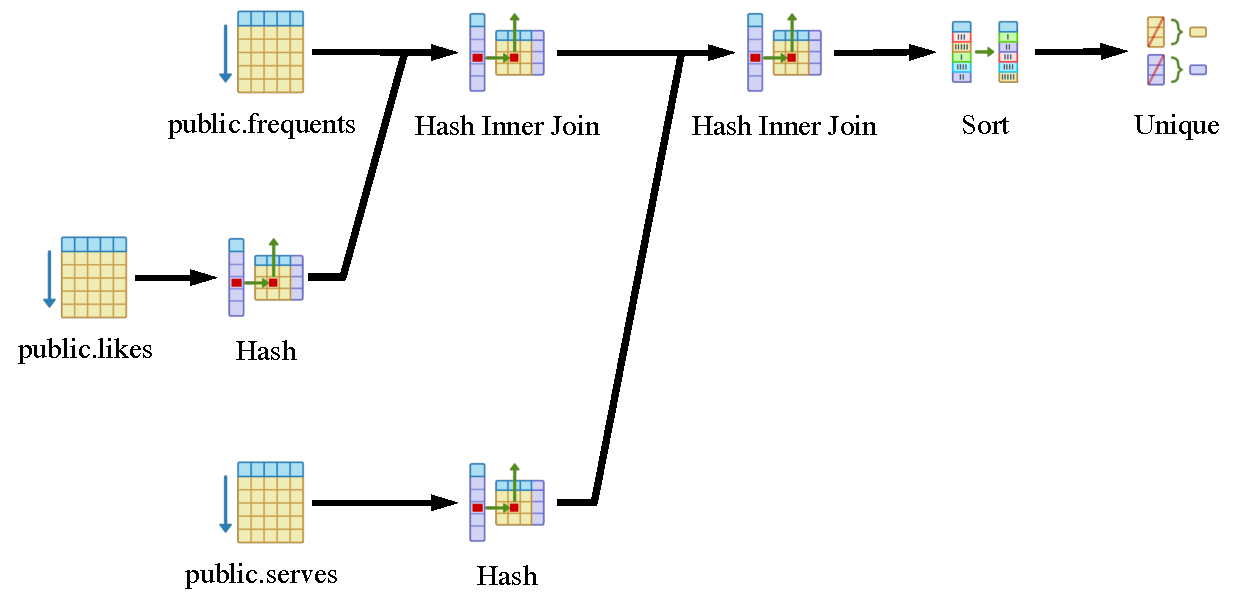
\includegraphics[scale=0.5]{figs/Fig_explain_PersonBarDrink}
	    \label{Fig_explain_PersonBarDrink}
	}
	\hfill
	\subfloat[$Q_{\textrm{some}}$ in DFQL]{
	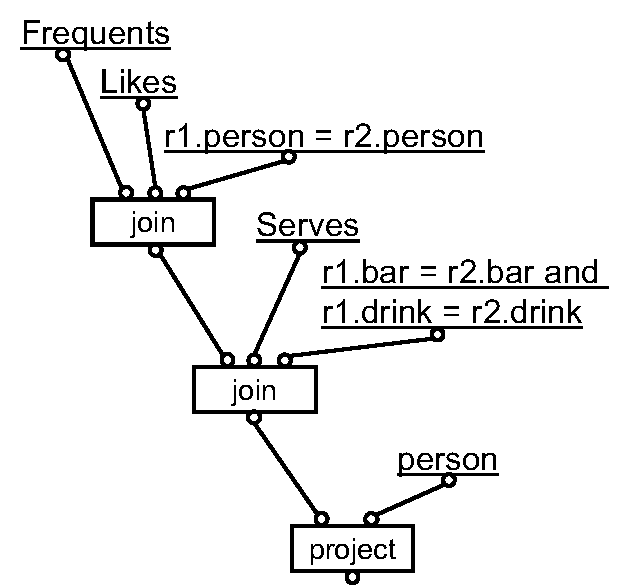
\includegraphics[scale=0.5]{figs/Fig_DFQL_Drinkers}
	    \label{Fig_DFQL_Drinkers}	
	}
    %
    %
    %
    %
    %
    %
    \caption{
	Query visualizations are not query plans nor data flow diagrams:
	(a) Visualized query plan by Postgres' EXPLAIN command~\cite{postgres} for query $Q_{\textrm{some}}$ from \autoref{figure:sql_conjunctive}.
	(b) Same query expressed in DFQL (Dataflow Query Language) \cite{DBLP:journals/iam/ClarkW94} which is modeled after relational algebra.
	Notice that neither visualization captures the cyclic nature of the joins 
	(see \autoref{Fig_ExampleExists}).
	%
	``\emph{Query visualization}'' to ``\emph{query plan visualization}'' 
	is the same as
	``\emph{intend of a query} (WHAT)'' to ``\emph{execution of a query} (HOW)''.
		} 
    \label{Fig_explain_PersonBarBeer}
\end{figure}




\subsection{Alternatives to Query Visualization for helping users understand existing queries} 
\label{section:alternatives}

There are three main alternative approaches for helping users understand existing queries:


\textbf{(1) Illustrating queries by examples}. 
Several papers suggest illustrating the semantics of operators in a data flow program or the semantics of queries by generating 
\emph{example input and output data}, and possibly \emph{intermediate data}.
The result is basically a list of tuples for each relational operator~\cite{DBLP:conf/uist/AbouziedHS12,
DBLP:journals/vldb/ChandraCKRS015,
GrustKRS2011:SQLdebugging,
DBLP:journals/tods/GrustR13,
DBLP:journals/pvldb/KhanX0H17,
MRJ:ExplainingWrongQueries:2019,
DBLP:conf/sigmod/OlstonCS09}.
%




	%
	%






\textbf{(2) Translating queries into Natural Language (NL)}.
Translating between SQL and NL is a heavily researched topic, and various ideas are proposed to explain queries in NL~\cite{DBLP:conf/inlg/GehrmannDER18,
DBLP:conf/nldb/Ioannidis08, 
DBLP:conf/icde/KoutrikaSI10,
DBLP:conf/cidr/SimitsisI09, 
DBLP:conf/emnlp/XuWWFS18}. 
Work in this area convincingly argues that automatically creating effective free-flowing text from queries is difficult and that the overall task is quite different from previous work on creating NL interfaces to DBMSs~\cite{Jarke:NL:1985}.
There is also recent work on translating query plans into NL~\cite{DBLP:conf/sigmod/WangBLJLC21}.





\textbf{(3) Pretty printing queries}.
Query editors for major DBMSs use 
\emph{syntax highlighting
and aligning} 
%
of query blocks and clauses. 
Pretty printers, such as sqlparse~\cite{sqlparse}, automatically arrange a SQL query in a supposedly easy-to-read form.
The most important dimensions are colors, capital vs.\ small letters, and indentation.



%
%
%
%
%
%
%
%
%
%
%
%
%
%



	%
	%
	%
	%
	%
	%
	%
	%
	%
	%
	%
	%
	%
	%
	%
	%
	%
	%
	%
	%


A key difference of alternatives to query visualization is 
that they are all inherently linear.
A list of tuples or a textual description do not readily reveal common logical pattern behind queries.
In particular, we are not aware of any SQL to NL tool available today that could translate our example from 
\autoref{fig:beerquery}
into an intuitive NL representation.
Patterns are naturally best shown visually,
%
and even the programming design patterns book~\cite{Gamma:1995ys} illustrates its patterns with intuitive diagrams.
A theory of relational query patterns, and a query-user interaction pattern inspired by ``mix-and-match'',
seems naturally supported by a visual approach.
	%
	%
	%
In addition, our recent work \cite{relationalDiagrams} has shown that certain types of relational patterns 
cannot be represented in an operator-style (thus sequential) model.


%











\section{Principles of Query Visualization and Design trade-offs} 
\label{sec:2}



%
%
The challenge of query visualization is to find appropriate visual metaphors 
that ($i$) allow users to quickly understand a query's intent, even for complex queries,
($ii$) can be easily learned by users,
and ($iii$) can be obtained from SQL by automatic translation, including a visually-appealing automatic arrangement of nodes of the visualization.
We believe that---with the right visual alphabet---users can learn to interpret visualized queries by seeing examples without much active focus. This is similar to what is known in language learning theory as the difference between the active and the generally larger passive vocabulary: Actively reproducing newly learned content is generally more difficult than passively recognizing such content. 


We next discuss the principles that led us to a particular design of a query visualization language (actually two variants, which we discuss later in more detail). We list those here to spark a healthy debate. Not all listed principles are universal, and deviations may lead to interesting alternative design decisions. These principles are also not MECE (Mutually Exclusive and Collectively Exhaustive), and some design decisions can be justified separately from other overlapping decisions.







\begin{figure}[tb]
\centering
\begin{bsubfloatrows}[\hspace{20mm}]
\bsubfloat[$Q_{\textrm{some}}$ in SQL]{%
	%
	\textup{\textsf{
	\footnotesize
	\setlength{\tabcolsep}{1mm}
	\begin{tabular}[t]{@{} l l l l l}
			& \\
			& \textcolor{blue}{select distinct} F.person\\
			& \textcolor{blue}{from}	Frequents F, Likes L, Serves S\\
			& \textcolor{blue}{where}	F.person = L.person \\ 
			& \textcolor{blue}{and}		F.bar = S.bar \\ 					
			& \textcolor{blue}{and}		L.drink = S.drink
	\end{tabular}
	}}	
	%
\label{figure:sql_conjunctive}	
}
\bsubfloat[$Q_{\textrm{some}}$ in \queryvis]{%
    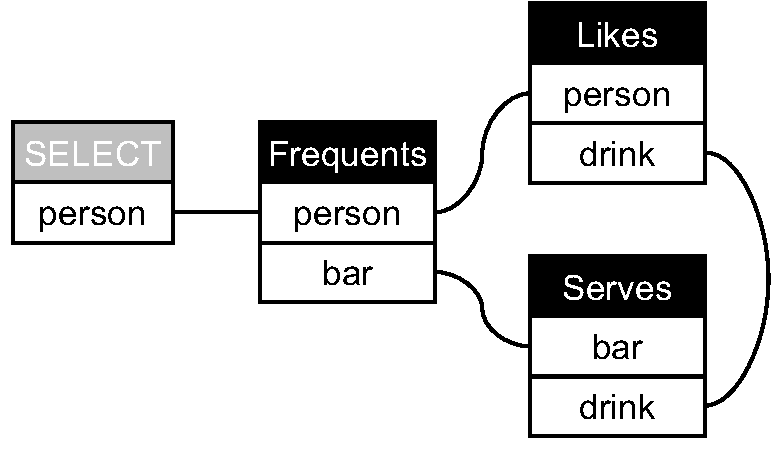
\includegraphics[scale=0.4]{figs/Fig_ExampleExists}
    \label{Fig_ExampleExists}
}
\end{bsubfloatrows}
\caption{Principles 1 \& 2:
Visualizing a conjunctive query should follow a familiar UML notation:
\emph{Find persons who frequent some bar that serves some drink they like}. 
The only novelty is a dedicated output table on the left,
emphasizing the compositionality of the relational model, 
and supporting an output-oriented reading order.
	%
	%
	%
	%
	%
	%
	%
	%
	%
	%
	%
	%
	%
	%
	%
	%
}
%
\end{figure}





\textbf{(1) Existing metaphors as starting point}: 
Ideally, a query visualization can be learned ``on-the-fly'' by seeing visualizations of increasing complexity, starting from examples that are already familiar.
Most database users are familiar with the UML diagram notation for classes and their attributes~\cite{folwer:UMLdistilled:2003}
applied to database schemas: Table names on top of column names in rectangular bounding boxes, 
primary-foreign keys contraints represented by lines between column names.
The visualization of a conjunctive query should thus not depart too much from 
such deeply familiar visual metaphors
%
(e.g., see the conjunctive query $Q_{\textrm{some}}$ in \autoref{figure:sql_conjunctive}
and its visualization in \autoref{Fig_ExampleExists}).
%
More complicated queries then progressively extend such familiar visual metaphors.




\begin{figure}[t]
\centering
 \parbox{.34\textwidth}{	
    \subfloat[$Q_{\textrm{only}}$]{
        %
		\textup{\textsf{
		%
		\footnotesize
		\setlength{\tabcolsep}{1mm}
		\begin{tabular}{@{} l l l l l}
		\\[17mm]			
			& \multicolumn{4}{l}{\textcolor{blue}{select distinct} F.person}\\
			& \multicolumn{4}{l}{\textcolor{blue}{from}		Frequents F}\\
			& \multicolumn{4}{l}{\textcolor{blue}{where}	not exists} \\ 
			& \phantom{xx}	& \multicolumn{3}{l}{(\textcolor{blue}{select} 	*}\\
			& 	 			& \multicolumn{3}{l}{\textcolor{blue}{from}		Serves S}\\
			& 	 			& \multicolumn{3}{l}{\textcolor{blue}{where}	S.bar = F.bar}\\
			& 	 			& \multicolumn{3}{l}{\textcolor{blue}{and}		not exists}\\
			&				& \phantom{xx}	& (\textcolor{blue}{select} 	L.drink \\
			&				& 				& \textcolor{blue}{from}	Likes L \\
			&				& 				& \textcolor{blue}{where} 	L.person = F.person \\
			&				& 				& \textcolor{blue}{and} 	S.drink = L.drink))		
		\\[15mm]
		\end{tabular}
		}}	
		\label{figure:sql_nested}
    }
    %
	%
}
 \parbox{.63\textwidth}{	
    \subfloat[$Q_{\textrm{only}}$]{
        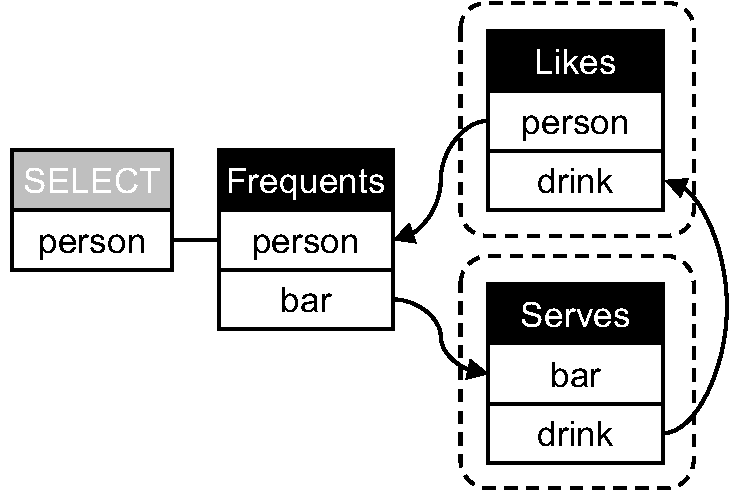
\includegraphics[scale=0.4]{figs/Fig_ExampleNotExists}
        %
        %
	}
    \hspace{1mm}
    \subfloat[$Q_{\textrm{only}}$]{
        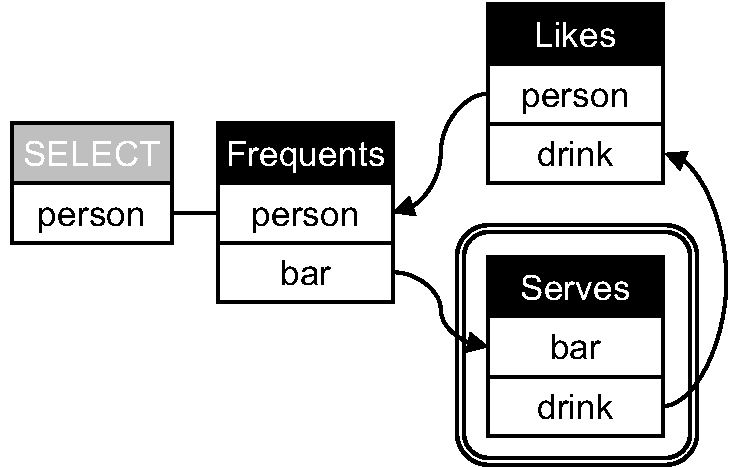
\includegraphics[scale=0.4]{figs/Fig_ExampleAll}
        %
        \label{Fig_ExampleAll}
	}
    \hspace{1mm}
    \subfloat[$Q_{\textrm{only}}$]{
        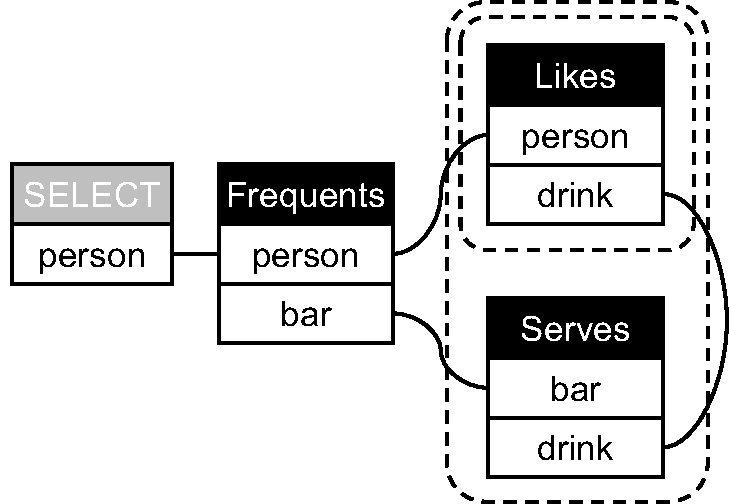
\includegraphics[scale=0.4]{figs/Fig_ExampleNotExistsRD}
        \vspace{1mm}
        \label{Fig_ExampleNotExistsRD}
	}
    \hspace{4mm}	
    \subfloat[$Q_{\textrm{only}}$]{
        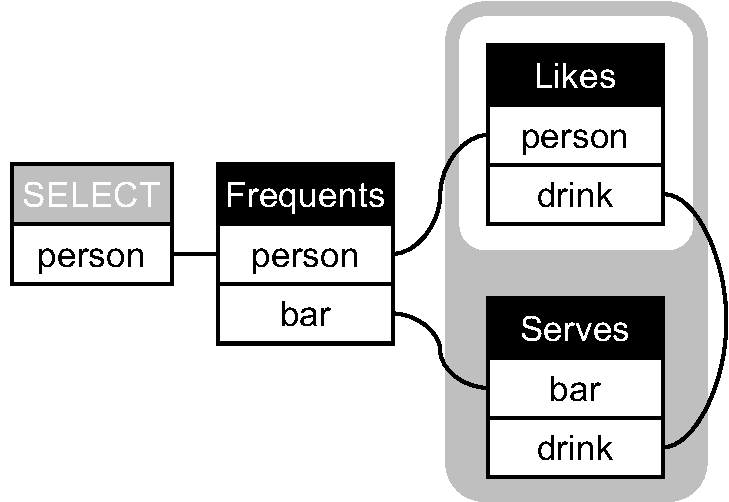
\includegraphics[scale=0.4]{figs/Fig_ExampleNotExistsRDShaded}
        \vspace{1mm}
        \label{Fig_ExampleNotExistsRDShaded}
	}		
}      
    \caption{
	Principles 3 \& 8:
	(a) \emph{Find persons who frequent some bar that serves 
	ONLY drinks they like}. 
	\queryvis:
	(b) Visualizing a nested query still follows familiar UML notations, 
	but now adds visual metaphors for $\nexists$ (dashed box) and 
	the reading order can be found by following the arrows.
	%
	%
	%
	%
	%
	%
	%
	%
	%
	(c) The reading can be further simplified by the use of the $\forall$ quantifier 
	(double-lined bounding box), a logical and intuitive operator that does not exist in SQL.
	The visualization asks for \emph{persons who frequent some bar so that 
	{ALL} drinks served are liked by them}.
	\diagrams are an alternative visualization that replaces arrows and reading orders by 
	explicit enclosure to express nesting relationships (d) and (e).
	}
    \label{Fig_ExampleVisualizations}
\end{figure}

%





\textbf{(2) Compositionality of the relational model}:
Inputs to queries are tables, and the output of a query is another table. 
Visualizations can (and we think should) emphasize this compositionality by explicitly showing an output table. 
This compositionality is also illustrated by the Relational Tuple Calculus expression for \autoref{figure:sql_conjunctive}:
\begin{align*}
	\{ q(\textit{person}) \mid \;
	& \exists f \in \textit{Frequents}, \exists l \in \textit{Likes}, \exists s \in \textit{Serves} 
	[
	q.\textit{person} = f.\textit{person} \wedge \\
	& 	
	f.\textit{person} = l.\textit{person} \wedge 
	l.\textit{drink} = s.\textit{drink} \wedge 	
	s.\textit{bar} = f.\textit{bar}
	] \}	
	%
\end{align*}
The expression makes use of 4 tables: 3 input tables (\textit{Frequents}, \textit{Likes}, and \textit{Serves}), and 1 output table called~$q$
(\autoref{Fig_ExampleExists} names the output table ``SELECT'').
In contrast, all interactive query tools listed in \autoref{sec:relatedWork} use either checkmarks, stars, or colors
%
to highlight a subset of attributes that are returned by the query.










\textbf{(3) Progressive visual complexity}: 
%
Entropy codes, such as Huffman codes~\cite{cover:thomas:2006}, 
compress data by encoding symbols with an amount of bits inversely proportional to the frequency of the symbols.
%
%
%
%
%
%
%
%
%
%
In the same spirit, a visual alphabet should be adapted to an overall expected workload and visual constructs for more common logical operators should be designed with lower visual complexity than less common ones. 
Starting from UML and its familiar notations for schemas and conjunctive queries, 
we can then enhance the visual representation in a \emph{progressive way}. 
For example, almost all database queries use the logical AND in their first-order logic translation (e.g.\ joins, \sql{EXISTS}, \sql{IN}), but only few use OR (e.g.\ \sql{OR}, \sql{UNION}). 
If infrequent query constructs become increasingly complex to read, this progression does not decrease the overall usability, but rather assures that more often used constructs are simple to read, in turn.
%
For example, the visualization of the query from \autoref{figure:sql_nested}
is expected to be at least as ``complicated'' as the query from \autoref{figure:sql_conjunctive}.

For increasing complexity of nested queries with negation, we are inspired by a body of work on \emph{diagrammatic reasoning systems}~\cite{DBLP:conf/iccs/Howse08}. 
Diagrammatic notations are in turn inspired by the influential \emph{existential graph notation} by Charles Sanders Peirce~\cite{peirce:1933,Roberts:1992,Shin:2002}.
These graphs exploit topological properties, such as enclosure, to represent logical expressions and set-theoretic relationships
%
%
(see description in \autoref{Fig_ExampleVisualizations}).






	%


	%









\textbf{(4) Expose (and not hide) relational patterns}:
We believe that a query visualization should expose the relational pattern used in a textual query,
instead of replacing it with an abstraction and concepts that go beyond the relational model.
This requires a visualization to use the same number of input tables of the textual query 
and to preserve a 1-to-1 mapping between them.
To illustrate, consider the SQL query in
\autoref{Fig_uniqueDrinkerTastSQL} asking for ``persons with a unique drink taste.''
The query uses 6 instances of the same table in a pattern that reads
``return any person, s.t.\ there does not exist any other person, s.t. there does not exist any drink liked by that other person 
that is not also liked by the returned person and there does not exist any drink liked by the returned person that is not also liked by the same other person.''
The visualization in \autoref{Fig_uniqueDrinkerTastQV1}
does not replace that relational pattern with another shorter construct, but rather 
makes it easier to inspect and reason about:
it complements the textual query
and preserves some traceable mapping between query and visualization. It preserves its relational pattern.







\begin{figure}[t]
\centering
\subfloat[SQL query]{
	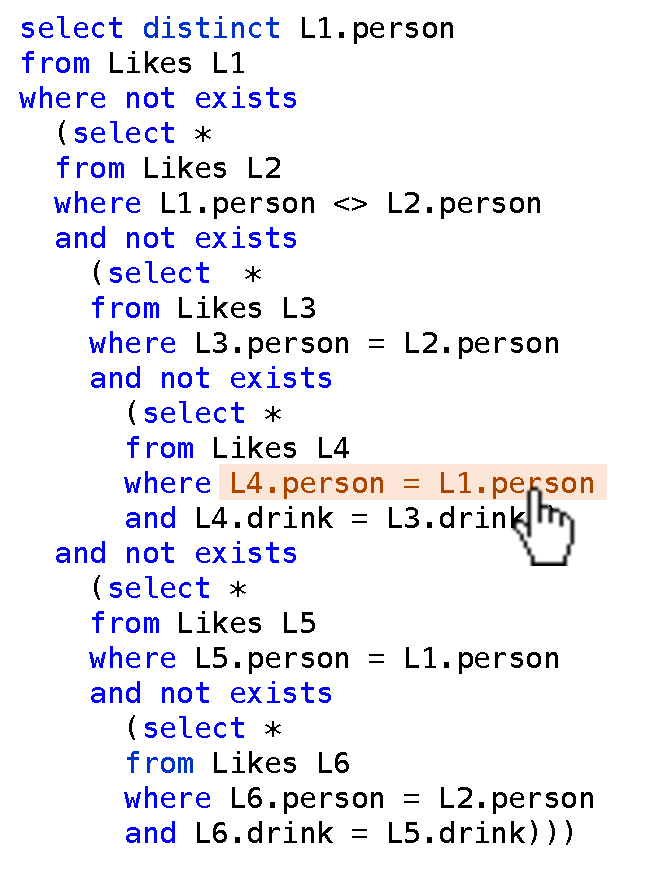
\includegraphics[scale=0.4]{figs/Fig_uniqueDrinkerTasteSQL}
	\label{Fig_uniqueDrinkerTastSQL}}
\hspace{10mm}
\subfloat[Query Visualization]{
	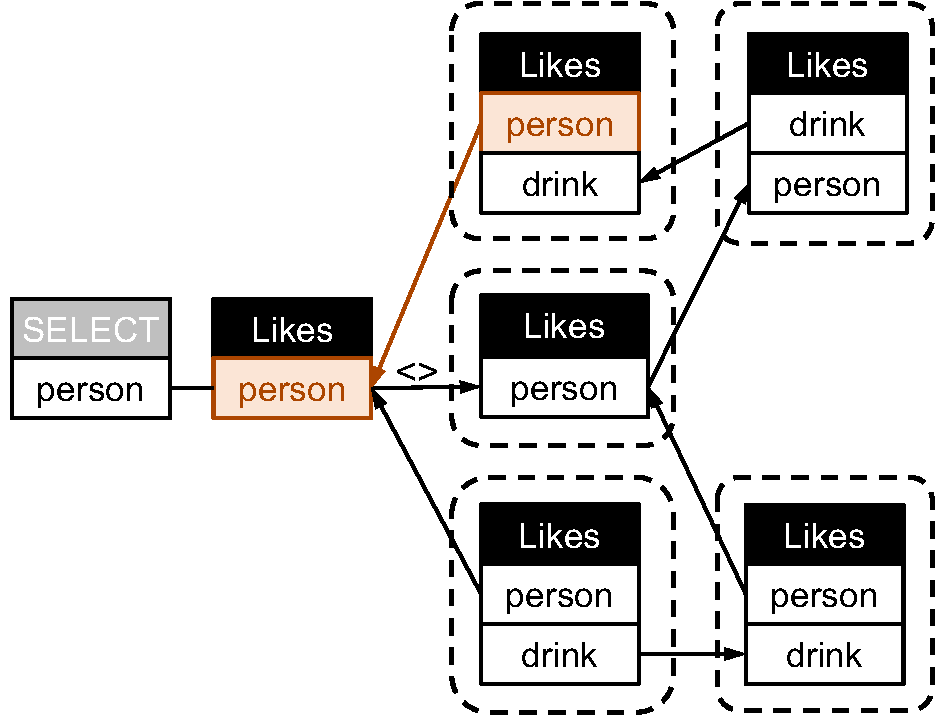
\includegraphics[scale=0.45]{figs/Fig_uniqueDrinkerTastQV1}
	\label{Fig_uniqueDrinkerTastQV1}}	
%
%
%
%
\caption{Principles 4 \& 5: 
(a) Unique-set-query ``\emph{Find person with a unique drink taste}.''
(b)~\queryvis diagram with reading order encoded by arrows 
(please see \cite{DBLP:conf/sigmod/LeventidisZDGJR20} for a detailed discussion of the query and its visualization).
There is a 1-to-1 correspondence between the SQL query and its visualization. 
As the user moves the mouse over fragments of the query, the graphical representation highlights the corresponding visual elements.
%
%
%
%
%
}
\label{fig:beerquery}
\end{figure}









\textbf{(5) Minimal visual complexity}: 
A query visualization should fulfill some kind of minimality criteria.
Intuitively, we aim to minimize the ink-data ratio 
(thus we like to maximize its inverse: Edward Tufte's famous data-ink ratio defined as the proportion of a graphic’s “ink” devoted to the informative and thus non-redundant display of data information~\cite{tufte2001visual}).
	%
	%
Minimality can be interpreted in different ways:
For example, the visual alphabet could contain only a minimal set of different visual elements; removing an element would then render the visualization less expressive.
Or, for a given query, removing a particular visual element would render the query incomplete.
To achieve such minimality, one can take inspiration by comparative analysis of existing textual languages.
For example, 
($i$) Datalog does not require the use of table aliases (different occurrences of the same input relation can be distinguished by their join patterns), whereas SQL requires alias.
On the other hand, ($ii$) SQL (inspired by tuple relational calculus) does not reference any attribute that is not used by the query,
whereas Datalog uses positional information and thus requires to maintain positional information.
\autoref{Fig_uniqueDrinkerTastQV1}
shows an example \queryvis visualization that combines the best of both worlds: 
($i$) repeated relations do not require aliases, 
and ($ii$) each of those occurrences only displays attributes needed.\footnote{A visualization could still show aliases to make it easier to maintain a static correspondence between the query and it visualization. However those aliases are not needed to interpret the meaning of a visual diagram.}

	%
	%
	%
	%
	%
	%
	%











\textbf{(6) Abstract away from syntax details}:
%
A query visualization abstracts away from language-specific peculiarities.
It can thus be non-injective with regard to syntactic redundancy.
A prominent example is SQL's use of NULLs. 
While there has been a lot of work on putting SQL's use of NULL values on solid foundations,
there is no universally agreed standard, and 
SQL queries evaluated on databases with NULL ``may produce answers that are just plain wrong''~\cite{DBLP:journals/sigmod/GuagliardoL17}.
The goal of query visualization can't be to provide an unambiguous interpretation of queries in the presence of NULLs, 
and thereby as a side-product also fix issues that have vexed database theoreticians over decades.
Rather, the focus of query visualization on the underlying relational patterns means that query visualizations 
need to abstract away from such oddities and not preserve them
(see \autoref{Fig_CompleteExampleAmbiguous}).
Also, a query visualization is meant to complement a textual original query.
It thus does not have to preserve all the information from the query; it can be non-injective,
thereby dividing the work: a visualization for the overall pattern, the text for the details.
This point goes back to \autoref{section:whatisQVnot} and what query visualization does not try to achieve.
	%
The focus is on WHAT a query does, 
yet confined to the relational model and the particular underlying relational pattern
(including all the input tables used), not the syntax nor the HOW of a particular execution plan.
Tools that help users cope with the inherent syntactic difficulty of SQL fall under the category of SQL debugging (\autoref{sec:querydebugging}).
The common foundation of all relational query languages and the relational model is
First-Order Logic.
%
%
%
%
We thus believe that focusing on the \emph{logical interpretation} of queries~\cite{DBLP:journals/bsl/HalpernHIKVV01} and set semantics 
provides a solid and well-understood foundation for query visualization.
See \autoref{Fig_CompleteExampleAmbiguous} for an example.





	%


	%
	%







	%
	%
	%
	%
	%
	%
	%
	%
	%
	%
	%
	%
	%
	%
	%
	%
	%
	%
	%
	%
	%
	%
	%
	%
	%
	%
	%
	%
	%
	%
	%
	%
	%
	%
	%
	%
	%
	%
	%
	%
	%
	%
	%
	%
	%
	%
	%
	%
	%
	%
	%
	%
	%
	%
	%
	%
	%
	%
	%






\begin{figure}[tb]
\centering
\begin{bsubfloatrows}[\hspace{20mm}]
\bsubfloat[]{%
	%
	\textup{\textsf{
	\footnotesize
	\setlength{\tabcolsep}{1mm}
	\begin{tabular}{@{} l l l l l}
	%
	%
		& \multicolumn{4}{l}{\textcolor{blue}{select distinct} A}\\
		& \multicolumn{4}{l}{\textcolor{blue}{from}		R}\\
		& \multicolumn{4}{l}{\textcolor{blue}{where}	B not in} \\ 
		& \phantom{xx}	& \multicolumn{3}{l}{(\textcolor{blue}{select} 	C}\\
		& 	 			& \multicolumn{3}{l}{\textcolor{blue}{from}		S)}
	\\[23mm]
	\\
	\end{tabular}
	}}	
	%
\label{Fig_IntroductionExample_b_table}	
}
\bsubfloat[]{%
	%
	\textup{\textsf{
	\footnotesize
	\setlength{\tabcolsep}{1mm}
	\begin{tabular}{@{} l l l l l}
	%
	%
		& \multicolumn{4}{l}{\textcolor{blue}{select distinct} A}\\
		& \multicolumn{4}{l}{\textcolor{blue}{from}		R}\\
		& \multicolumn{4}{l}{\textcolor{blue}{where}	not exists} \\ 
		& \phantom{xx}	& \multicolumn{3}{l}{(\textcolor{blue}{select} 	*}\\
		& 	 			& \multicolumn{3}{l}{\textcolor{blue}{from}		S}\\
		& 	 			& \multicolumn{3}{l}{\textcolor{blue}{where}	B=C)}		
	%
	\\
	\end{tabular}
	}}	
	%
\label{Fig_IntroductionExample_c_table}
}
\bsubfloat[]{%
    %
	\begin{minipage}{45mm}	
	\vspace{5mm}
	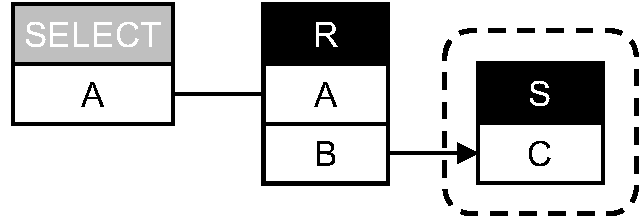
\includegraphics[scale=0.4]{figs/Fig_ExampleNotExistsv2}
	\end{minipage}
	%
    \label{Fig_ExampleNotExists}
}
\end{bsubfloatrows}
\caption{Principles 6 \& 7: Queries (a) and (b) are equivalent except if column S.C contains NULL values. 
Thus ignoring NULL values in the database, they are equivalent and their \emph{query intent} can be represented by the same 
\queryvis representation shown in (c)
(example taken and slightly fixed from Fig.~4 in \cite{gatterbauer2011databases}).}
\label{Fig_CompleteExampleAmbiguous}
\end{figure}







\textbf{(7) Output-oriented reading order}:
Similar to a SQL query having an expected order of clauses (e.g.\ SELECT-FROM-WHERE),
also a query visualization benefits from having an expected arrangement and reading order.
Mirroring the design decision from SQL and calculus, we suggest a reading order left-to-right 
that starts with the result of the query (the output table) 
and then adds tables in horizontal layers in decreasing order of their relatedness to the output table (see \autoref{Fig_ExampleNotExists}). 
This suggests an arrangement where the input tables are placed at a horizontal distance from the output table that represents the shortest path join connection to the output table.
Furthermore, the arrangement of the input tables should 
be such as to simplify the reading and understanding of the query 
by following aesthetic heuristics (e.g.\ minimizing the number of line crossings).






\textbf{(8) Logic-based visual transformations}:
Nested negated quantifiers are particularly difficult to understand for users~\cite{DBLP:journals/csur/Reisner81,Reisner1975:HumanFactors}.
Simple visualizations of logical transformation can further help show the query in a more intuitive form.
Take a double negated query such as \autoref{Fig_ExampleVisualizations}:
\begin{align*}
	\{ q(\textit{person}) \mid \;
	& \exists f \in \textit{Frequents}
	[
	q.\textit{person} = f.\textit{person} \wedge
	\neg \exists s \in \textit{Serves} [s.\textit{bar} = f.\textit{bar} \wedge
	\\
	&\neg \exists l \in \textit{Likes} [
	l.\textit{drink} = s.\textit{drink} \wedge 	
	f.\textit{person} = l.\textit{person}	
	] \}	
\end{align*}
The same query can be arguably understood more easily by writing it as
\begin{align*}
	\{ q(\textit{person}) \mid \;
	& \exists f \in \textit{Frequents}
	[
	q.\textit{person} = f.\textit{person} \wedge
	\forall s \in \textit{Serves} [s.\textit{bar} = f.\textit{bar} \rightarrow
	\\
	&\exists l \in \textit{Likes} [
	l.\textit{drink} = s.\textit{drink} \wedge 	
	f.\textit{person} = l.\textit{person}	
	] \}	
\end{align*}



















%
\section{Our Suggestions: \queryvis and \diagrams}

When following the earlier listed design principles, a family of query visualizations naturally emerges.
%
We discuss here two instances that differ in the way they visually encode the \emph{nesting structure between query blocks}:

(1) \queryvis~\cite{DanaparamitaG2011:QueryViz,
gatterbauer2011databases,
DBLP:conf/sigmod/LeventidisZDGJR20}:
This earlier variant from 2011
%
%
%
borrows the idea of a ``default reading order''
from diagrammatic reasoning systems~\cite{DBLP:conf/diagrams/FishH04} 
and uses \emph{arrows} to indicate an implicit reading order between different nesting levels.
Take as example~\autoref{Fig_ExampleNotExists} and notice how the arrows between the relations correspond to the order in which 
they appear in the natural language translation
(``Find persons who FREQUENT some bar that SERVES only drinks they LIKE''). 
Without the arrows, there would be no natural order placed on the existential quantifiers 
and the visualization would be ambiguous.
\queryvis focuses on the non-disjunctive fragment of relational calculus and is guaranteed to represent connected nested queries unambiguously up to nesting level 3.
An interactive online version is available linked from \url{https://queryvis.com}.
	%
	%
	%
	%
	%



(2) \diagrams~\cite{relationalDiagrams}:
This more recent variant indicates the nesting structure of table variables by using \emph{nested negated bounding boxes} instead of arrows.
 %
The nesting of negation boxes is more closely inspired by Peirce's influence beta existential graphs~\cite{peirce:1933,Roberts:1992,Shin:2002}.
%
%
Interestingly, because \diagrams are based on Tuple Relational Calculus (instead of Domain Relational Calculus which is closer to First-Order Logic)
they solve interpretation problems of beta graphs that have been the focus of intense research in the diagrammatic reasoning communities.
The big advantage of this variant is that it has a provably unambiguous interpretation for any nesting depth, 
even for queries with disconnected components,
and for both Boolean and non-Boolean queries.
Furthermore, by adding one additional visual element, \diagrams can be made relationally complete even for non-Boolean queries.
The downside is that these diagrams need more ``ink'' for simple nested queries, 
and logical transformations (design decision 8) cannot be as easily applied anymore.
An alternative to such transformations, however, is using shading for alternating nesting depths
(see e.g.\ \autoref{Fig_ExampleNotExistsRDShaded}).



An interactive online version of \queryvis has been online at \url{https://queryVis.com} since 2011~\cite{DanaparamitaG2011:QueryViz}.
We encourage the reader to try it. 
It currently supports only a limited SQL grammar (see the web page for details). 
Still, this online demo shows that query visualization can have a very lightweight interaction. 
The user does not have to specify anything upfront and can just copy the SQL query and the schema into the two available forms
(notice that the relevant part of the schema could often be inferred from the query). 
	%





	%


	%
	%
	%
	%
	%
	%
	%
	%



	%
	%
	%
	%

	%
	%
	%
	%
	%










\subsection{User study showing users can interpreting queries faster with $\queryvis$}
\label{sec:userstudy}



We designed a user study to test whether our diagrams help users understand SQL queries \emph{in less time} and \emph{with fewer errors}, on average.
The study design and analysis plan was preregistered before we started the experiment and gathered data.  
Details on the study are available 
in \cite{DBLP:conf/sigmod/LeventidisZDGJR20} 
and on OSF at \osfprereg.


\begin{figure}[t]
\centering
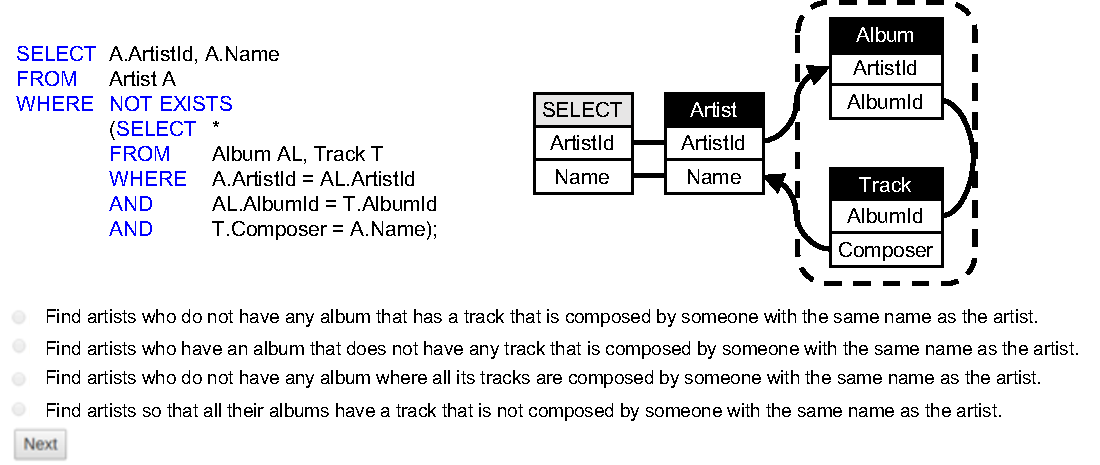
\includegraphics[scale=0.6]{figs/study_screenshot_v6.pdf} 
\caption{
	\autoref{sec:userstudy}: 
	Example query from our user study.
    The query is shown in the \emph{Both} condition, in which a participant sees the query in both SQL (left) and 
	our \queryvis diagram (right).
	%
	}
\label{figure:study_screenshot}
\end{figure}


The study is an easily-scalable \emph{within-subjects study}~\cite{seltman2012experimental} 
(i.e., all study participants were exposed to all query interfaces).
%
%
%
The study consisted of 9 multiple-choice questions (MCQs).
 %
Each MCQ asked the participant to choose the best interpretation for a presented query from 4 choices.
Following best practices in MCQ creation~\cite{Zimmaro2010},
we created all 4 choices to read very similar to each other so that a participant with little knowledge of SQL would be incapable of eliminating any of the 4 choices.
Each query was presented to participants in one of 3 conditions: 
(1) seeing a query as SQL alone (``SQL''), 
(2) seeing a query as a logical diagram that was generated from SQL (``QV''), or 
(3) seeing both SQL and \queryvis at the same time (``Both'').
\autoref{figure:study_screenshot} shows the interface for the condition ``Both'' for one of the 9 questions.
Each participant answered \emph{all 9 questions in the same order} but
the condition for each question was 
randomized in a particular way that reduces potential biases in our analysis due to condition ordering effects
following a \emph{Latin square design}~\cite{Ledolter:2007fu,Montgomery:2013wq}.
We then tracked the time needed and errors made by each participant while trying to find the correct interpretation for each query.
%
%
%
Participants had to pass an SQL qualification exam to ensure that they had at least a basic proficiency with SQL.
We made the study available for 3 weeks from Jan 24, 2020--Feb 13, 2020 on Amazon Mechanical Turk (AMT),
during  which we recruited $n = 42$ legitimate participants.


\introparagraph{Results}
There is strong evidence that participants are meaningfully faster (-20\%) using \queryvis than {SQL} 
($p<0.001$). 
There is weak evidence that participants make meaningfully fewer errors (-21\%) using \queryvis than {SQL}
($p=0.15$).
\autoref{figure:differences_no_grouping}
shows the full time and error difference distribution across the 42 participants.








\begin{figure}[t]
\centering
\subfloat[]{
    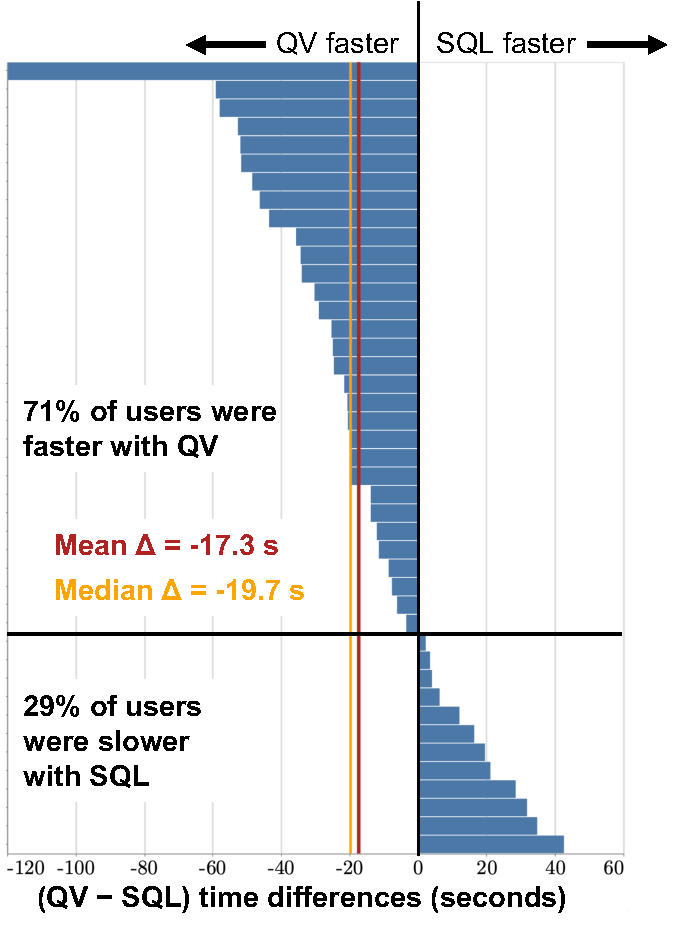
\includegraphics[scale=0.44]{figs/Fig_time_differences_no_grouping_v2.pdf}
    \label{figure:time_differences_no_grouping}
}
\hspace{25mm}
\subfloat[]{
    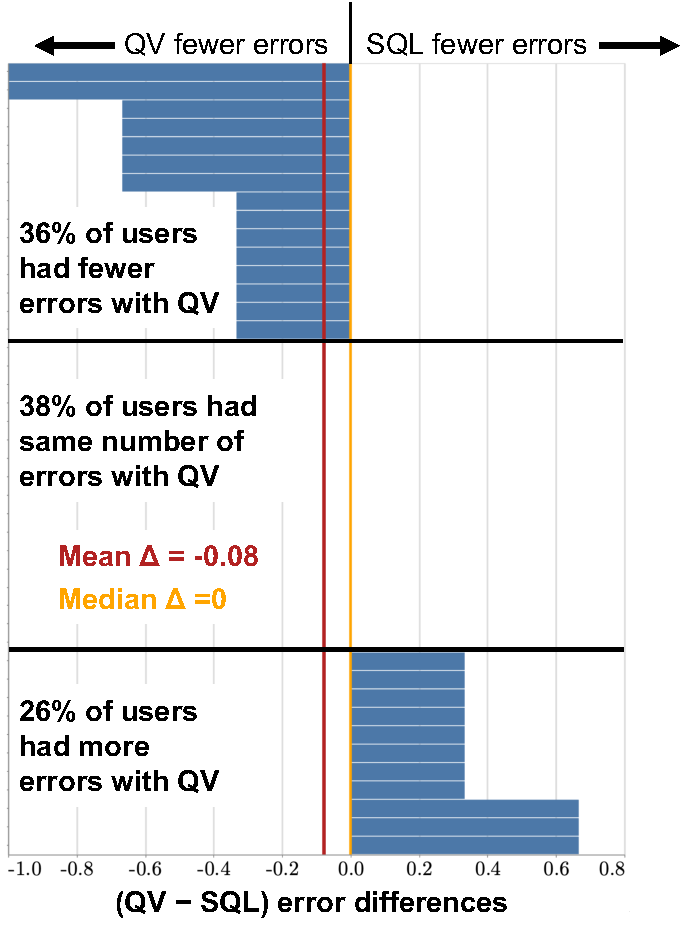
\includegraphics[scale=0.44]{figs/Fig_error_differences_no_grouping_v2.pdf}
	\label{figure:error_differences_no_grouping}
}
\caption{\autoref{sec:userstudy}:
Distribution of (QV$-$SQL) time and error differences for each participant on 9 MCQs.
}
\label{figure:differences_no_grouping}
\end{figure}













	%
	%
	%
	%
	%
	%
	%
	%
	%
	%
	%
	%
	%
	%
	%
	%
	%
	%
	%
	%
	%
	%
	%
	%
	%
	%
	%
	%
	%
	%
	%
	%



	%
	%
	%
	%
	%
	%
	%
	%
	%
	%
	%
	%
	%
	%
	%
	%
	%
	%
	%
	%
	%
	%
	%
	%
	%
	%
	%
	%
	%
	%
	%
	%
	%
	%
	%
	%
	%
	%
	%
	%
	%



	%
	%
	%
	%
	%
	%
	%
	%
	%
	%
	%
	%














\section{Related work}
\label{sec:relatedWork}





For decades, SQL has been the main standard for issuing queries over relational databases.
There is a reasonable chance that this widely implemented interface won't be replaced anytime soon. 
Thus we do not propose new ways to write queries, 
but instead explore how to help users \emph{understand existing SQL queries}. 


\introparagraph{Visual Query Languages (VQL)}
Visual methods for expressing queries have been studied
extensively in the database literature~\cite{DBLP:journals/vlc/CatarciCLB97}, 
%
%
and
many commercial database products offer some visual interface for users to write simple SQL queries.
Query Visualization (QV) focuses on the problem of describing and \emph{interpreting a query that has already been written}, which is 
different from the problem of composing a new query (\autoref{QVisnotVQL}).



	%
	%





	%
	%
	%
	%
	%
	%

	%
	%
	%
	%
	%
	%
	%
	%
	%
	%
	%
	%

    %
    %






	%
	%
	%
	%
	%
	%
	%
	%
	%
	%
	%
	%



%
%
%



\textbf{Interactive query builders} employ 
visual diagrams that 
%
users can manipulate (most often in order to select tables and attributes)
%
while using \emph{a separate query configurator}
%
(similar to QBE's condition boxes~\cite{DBLP:journals/ibmsj/Zloof77}) 
to specify selection predicates, attributes, and sometimes nesting between queries.
dbForge~\cite{dbforge} is the most advanced and commercially supported tool we found for interactive query building.
Yet it does not show any visual indication for non-equi joins between tables 
and the actual filtering values and aggregation functions can only be added in a separate query configurator.
Moreover, it has limited support for nested queries: 
the inner and outer queries are built separately,
and the diagram for the inner query is \emph{presented separately and disjointly} 
from the diagram for the outer query.
Thus  \emph{no visual depiction of correlated subqueries is possible}.
%
Other graphical SQL editors like SQL Server Management Studio (SSMS)~\cite{ssms}, Active Query Builder~\cite{activequerybuilder}, QueryScope from SQLdep~\cite{queryscope}, MS Access \cite{msAccess}, and
PostgreSQL's pgAdmin3~\cite{pgadmin} lack in even more aspects of visual query representations: 
most do not allow nested queries, 
none has a single visual element for the logical quantifiers 
\texttt{NOT} \texttt{EXISTS} or \texttt{FOR} \texttt{ALL},
and all require specifying details of the query in SQL or across several tabbed views 
\emph{separate from a visual diagram}.
%
%
%
%
%
%
DataPlay~\cite{DBLP:conf/uist/AbouziedHS12} 
allows a user to specify their query by interactively modifying a \emph{query tree with quantifiers}
and observing changes in the matching/non-matching data.
%
%
%
%
%
%
	%
	%
	%
	%
	%
	%
	%
	%
%
Gestural query specification~\cite{10.14778/2732240.2732247}
allows a user to query databases using a series of gestures on a touchscreen.
In short, current graphical SQL editors \emph{do not provide a single encompassing visualization of a query}.
%
%
%
%
Thus they could not (even in theory) transform a complicated SQL query
into a single visual representation, which is the focus of query visualization.
%
%

 %





	%
	%

	%
	%
	%

	%
	%


	%
	%

	%
	%
	%
	%
	%
	%
	%

	%
	%
	%
	%
	%
	%
	%
	%
	%
	%
	%
	%
	%
	%
	%
	%
	%

	%
	%

	%
	%
	%
	%
	%
	%

%
%
%
%







\textbf{Query visualizations}
%
%
%
%
attempt to create succinct visual representations of existing queries.
%
%
This explicit reverse functionality for SQL has not drawn as much attention as visual query builders,
and there are only a handful of other systems we are aware of~\cite{gatterbauer:diagrams:tutorial:2022}.
%
%
Visual SQL~\cite{DBLP:conf/er/JaakkolaT03} is 
a visual query language that also support query visualization. 
With its focus on query specification, it maintains the one-to-one correspondence to SQL,
and syntactic variants of the same query lead to different representations (\autoref{Fig_CompleteExampleAmbiguous}).
SQLVis~\cite{DBLP:conf/vl/MiedemaF21} shares motivation with \queryvis. 
Similar to Visual SQL, it places a stronger focus on the actual syntax of a SQL query 
and syntactic variants like nested EXISTS queries change the visualization.
%
%
%
%
%
Snowflake join~\cite{snowflakejoin} is an open source project that visualizes join queries with optional grouping.
It does not have any consistent and unambiguous notation for nested queries.
%
GraphSQL~\cite{DBLP:conf/dexaw/CerulloP07} uses visual metaphors that are different from typical relational schema notations 
%
%
and visualizations, even simple conjunctive queries can look unfamiliar.
%
The Query Graph Model (QGM) developed for Starburst~\cite{DBLP:conf/sigmod/HaasFLP89}
helps users understand query plans, not query intent (\autoref{sec:queryplans}).
%
StreamTrace \cite{DBLP:conf/chi/BattleFDBCG16}
focuses on visualizing temporal queries
%
with
	 %
	%
workflow diagrams and a timeline.
It is an example of visualizations for spatio-temporal domains and not the logic behind general relational queries.


	%
	%
	%
	%
	%
	%
	%
	%
	%
	%
	%
	%
	%
	%
	%
	%
	%
	%
	%
	%
	%
	%
	%
	%
	%
	%
	%
	%
	%
	%
	%
	%
	%





	%
	%
	%
	%
	%
	%
	%
	%
	%
	%
	%
	%
	%
	%
	%
	%
	%
	%
	%
	%
	%
	%
	%
	%
	%
	%
	%
	%
	%
	%
	%
	%
	%
	%
	%
	%
	%

	%
	%
	%
	%
	%
	%
	%
	%
	%
	%





	%






	%
	%
	%



	%
	%
	%
	%
	%
	%
	%
	%
	%
	%
	%
	%
	%
	%
	%
	%
	%
	%
	%






%
%
%
%
%
%
%










\section{Various Challenges} 


A vision paper that some of us wrote in 2011 declared that ``Databases will visualize queries too''~\cite{gatterbauer2011databases}.
This has not yet widely happened.
Why so? Is it just a matter of time?  Or is it that we are missing something profound and Queries Visualizations (QV) will go the same route as Visual Query Languages (VQL):
intuitively attractive, but practically not as useful?
%
Instead, perhaps the foundations have been laid, yet there are still problems to be solved
to make that vision practical.
Here is a partial list of several such challenges:

%



\textbf{(1) Extensions}:
Expressing logical disjunction in diagrams is inherently more complicated than conjunction~\cite{Shin:2002}.
And while relational algebra, relational calculus, and Datalog all use set semantics, SQL uses bag semantics.
What are \emph{appropriate visual metaphors} for 
general disjunctions 
and non-logical constructs, such as 
groupings, aggregates, arithmetic predicates, bag semantics, outer joins, null values, and recursion?\footnote{The online \queryvis interface at \url{https://queryVis.com} has been quietly supporting limited forms of aggregates already since 2016.}



\textbf{(2) Relational patterns}:
Something not well understood or even formalized today is the vague concept of ``relational query patterns.''
What are query patterns?
	%
	%
	%
	%
We posit that identifying patterns in queries may have several advantages, 
akin to how formalizing best practices in software design patterns has aided software engineers \cite{Gamma:1995ys}.
General and reusable query patterns could assist in teaching students how to write complicated queries.
Queries written using common patterns could then potentially be easier to interpret quickly.
What is \emph{a rigorous semantic definition of relational query patterns}?
See \cite{relationalDiagrams} for first steps in that direction.



\textbf{(3) Measures of visual conciseness}: 
We listed minimal visual complexity as guiding principle. 
When comparing two languages one could likely develop metrics such as amount of ink used.
However, what is the ultimately right measure for quantifying visual complexity for a human user?
	%
Visual complexity also needs to take into account prior familiar notions (like UML) to a target audience.






\textbf{(4) Automatic layout algorithms}:
The online \queryvis demo uses a layered arrangement of tables that guarantees that any join conditions
are either between two adjacent layers or within the same layer.
It uses the standard Graphviz library for arranging the tables and their attributes~\cite{Ellson03graphvizand}.
However, existing graph layout algorithms are not suited for complicated layered graphs with nested hierarchies.
What are new outline algorithms that can optimize for existing visual metrics (such as minimum line overlap) 
and define novel metrics that capture visual homogeneity?
A possible route is 
encoding existing aesthetic heuristics (such as those in \cite[Table 1]{DBLP:conf/cae/BennettRSG07})
or novel ones
in quantitative metrics, and then
defining the layout problem as Integer Linear Program (ILP). 
A recent proposal that uses this route is STRATISFIMAL LAYOUT~\cite{DBLP:journals/tvcg/BartolomeoRGD22}.







\textbf{(5) Interactive diagrams}:
As already implied by \autoref{Fig_KevinBacon},
\autoref{Fig_TheVision}, 
\autoref{Fig_SpeechAssistant},and
\autoref{fig:beerquery},
the interaction between textual query and query visualization could be more involved beyond a simple one-way translation.
Interactive mouse-over can show correspondences. 
%
An interactive auto-complete feature could suggest possible query templates. 
And a user could be allowed to manipulate an existing template of a query, which then gets reflected in the text
(but notice that this last point would defeat the original idea to keep the visualization lightweight and as easy add-on to an existing query composition workflow).
What is the optimal end-to-end integration of visualization and text or alternative input forms
(recall \autoref{Fig_SpeechAssistant} and \autoref{Fig_TheVision})?


	%


\textbf{(6) Combinations with other modalities}:
We mentioned in \autoref{section:alternatives} alternative ways to help users understand their queries.
Such alternative modalities could possibly be combined with visualizations.
For example, Natural Language translations could possibly benefit from a graphical representation of a query.
Parts of a query could be replaced with an automatically created text and expanded with a click to the full pattern.
Query visualizations could be enhanced with example database instances, or operator-by-operator translations.
The query visualizations could be modified to display how individual records fit or don’t fit the query. 
This could again be done with interactive mouseover or choice from a menu.



\textbf{(7) User studies}: 
We believe that preregistered, within-subjects studies with multiple-choice questions in Latin square design studies, 
where the correctness of a user's answer can be determined automatically,
are the way to go to for easily scalable quantitative comparison between different interfaces. 
In our user study, users needed to pass a SQL qualifying exam and then started the test only after minimum exposure to \queryvis. 
One could only imagine the improvement after the users had chance to become more familiar with the visual language over an extended period of time.
 %
For such a longitudinal study that possibly instruments across control groups there is one big open challenge:
How to parameterize SQL queries and questions in the spirit of Gradiance
\cite{gradiance}
such that the same subjects can take the same test repeatedly?
Such new user study paradigms would allow us 
to observe the improvement in speed and accuracy over an extended period of time.


%

%



%
%
%
%
%
%
%
%
%
%






\textbf{(8) Declarative programming}:
Logical query interfaces have shown success also beyond relational data.
Examples include Datalog for networks
\cite{DBLP:conf/sigmod/HuangGL11,DBLP:journals/cacm/LooCGGHMRRS09,DBLP:conf/sosp/LooCHMRS05}
and Inductive Logic Programming~\cite{SchmidMuggleton:2017}. 
Such programs represent an explicit symbolic structure that can be inspected and understood, and the implied logic visualized.



	%
	%













\section{Conclusions and Future Work} 
\label{sec:conclusions_and_future_work}

We discussed the potential of query visualizations for a future, advanced user-query interaction
that visualizes relational patterns of a query with diagrams.
We delineated query visualization from visual query languages,
discussed a few principles for designing intuitive visual diagrams,
and gave two variants of a family of query visualizations.
Future work needs to  extend visual formalisms for the full relational model and beyond,
find algorithms for automatic arrangement of diagrams,
study novel and more interactive user interfaces 
with query visualizations being just one component, 
create more easily verifiable, large-scale user studies,
and find ways to apply logical representations to other logic-based languages such as Inductive Logic Programming.





\subsection*{Acknowledgements} 

This research is supported in part by NSF awards IIS-1762268, IIS-1956096, and IIS-2145382.
WG would also like to thank \href{https://www.linkedin.com/in/danaparamita/}{Jonathan Danaparamita} 
who created the original interactive QueryVis demo that has been online at 
\url{https://queryvis.com/} since 2011 and
without whom there would have been no \queryvis. 







\bibliographystyle{abbrv}
%

\begin{thebibliography}{100}

\bibitem{DBLP:conf/uist/AbouziedHS12}
A.~Abouzied, J.~M. Hellerstein, and A.~Silberschatz.
\newblock Dataplay: interactive tweaking and example-driven correction of
  graphical database queries.
\newblock In {\em Proceedings of the 25th annual ACM symposium on User
  interface software and technology ({UIST})}, pages 207--218, 2012.
\newblock \url{https://doi.org/10.1145/2380116.2380144}.

\bibitem{activequerybuilder}
{Active Query Builder}.
\newblock \url{https://www.activequerybuilder.com/}, 2019.

\bibitem{Ahmed2015}
T.~M. Ahmed, W.~Shang, and A.~E. Hassan.
\newblock An empirical study of the copy and paste behavior during development.
\newblock In {\em 2015 IEEE/ACM 12th Working Conference on Mining Software
  Repositories}, pages 99--110, 2015.
\newblock \url{https://doi.org/10.1109/MSR.2015.17}.

\bibitem{QueRIERecommendations:2010}
J.~Akbarnejad, G.~Chatzopoulou, M.~Eirinaki, S.~Koshy, S.~Mittal, D.~On,
  N.~Polyzotis, and J.~S.~V. Varman.
\newblock {SQL} {QueRIE} recommendations.
\newblock {\em PVLDB}, 3(1):1597--1600, 2010.
\newblock \url{https://doi.org/10.1145/2839509.2844640}.

\bibitem{ARZAMASOVA2021101646}
N.~Arzamasova and K.~B{\"o}hm.
\newblock Scalable and data-aware sql query recommendations.
\newblock {\em Information Systems}, 96:101646, 2021.
\newblock \url{https://doi.org/10.1016/j.is.2020.101646}.

\bibitem{DBLP:journals/tvcg/BartolomeoRGD22}
S.~D. Bartolomeo, M.~Riedewald, W.~Gatterbauer, and C.~Dunne.
\newblock {STRATISFIMAL} {LAYOUT:} {A} modular optimization model for laying
  out layered node-link network visualizations.
\newblock {\em {IEEE} Transactions on Visualization and Computer Graphics},
  28(1):324--334, 2022.
\newblock \url{https://doi.org/10.1109/TVCG.2021.3114756},
  \url{https://visdunneright.github.io/stratisfimal/}.

\bibitem{10.1145/3503490}
L.~Battle.
\newblock Analyzing online programming communities to enhance visualization
  languages.
\newblock {\em Interactions}, 29(1):27--29, jan 2022.
\newblock \url{https://doi.org/10.1145/3503490}.

\bibitem{DBLP:conf/chi/BattleFDBCG16}
L.~Battle, D.~Fisher, R.~DeLine, M.~Barnett, B.~Chandramouli, and J.~Goldstein.
\newblock Making sense of temporal queries with interactive visualization.
\newblock In {\em Proceedings of the 2016 CHI Conference on Human Factors in
  Computing Systems}, pages 5433--5443, 2016.
\newblock \url{https://doi.org/10.1145/2858036.2858408}.

\bibitem{DBLP:conf/cae/BennettRSG07}
C.~Bennett, J.~Ryall, L.~Spalteholz, and A.~Gooch.
\newblock The aesthetics of graph visualization.
\newblock In {\em 3rd International Symposium on Computational Aesthetics in
  Graphics, Visualization, and Imaging (CompAesth)}, pages 57--64. Eurographics
  Association, 2007.
\newblock \url{https://doi.org/10.2312/COMPAESTH/COMPAESTH07/057-064}.

\bibitem{Brandt2009}
J.~Brandt, P.~J. Guo, J.~Lewenstein, M.~Dontcheva, and S.~R. Klemmer.
\newblock Writing code to prototype, ideate, and discover.
\newblock {\em IEEE Software}, 26(5):18--24, 2009.
\newblock \url{https://doi.org/10.1109/MS.2009.147}.

\bibitem{DBLP:reference/db/Catarci18a}
T.~Catarci.
\newblock Visual query language.
\newblock In {\em Encyclopedia of Database Systems, Second Edition}. Springer,
  2018.
\newblock \url{https://doi.org/10.1007/978-1-4614-8265-9\_448}.

\bibitem{DBLP:journals/vlc/CatarciCLB97}
T.~Catarci, M.~F. Costabile, S.~Levialdi, and C.~Batini.
\newblock Visual query systems for databases: A survey.
\newblock {\em Journal of Visual Languages and Computing}, 8(2):215--260, 1997.
\newblock \url{https://doi.org/10.1006/jvlc.1997.0037}.

\bibitem{DBLP:conf/dexaw/CerulloP07}
C.~Cerullo and M.~Porta.
\newblock A system for database visual querying and query visualization:
  Complementing text and graphics to increase expressiveness.
\newblock In {\em International Workshop on Database and Expert Systems
  Applications (DEXA)}, pages 109--113. {IEEE}, 2007.
\newblock \url{https://doi.org/10.1109/DEXA.2007.91}.

\bibitem{ChanUserDatabaseInterface:1993}
H.~C. Chan, K.~K. Wei, and K.~L. Siau.
\newblock User-database interface: The effect of abstraction levels on query
  performance.
\newblock {\em MIS Quarterly}, 17(4):441--464, 1993.
\newblock \url{https://doi.org/10.2307/249587}.

\bibitem{DBLP:journals/vldb/ChandraCKRS015}
B.~Chandra, B.~Chawda, B.~Kar, K.~V.~M. Reddy, S.~Shah, and S.~Sudarshan.
\newblock Data generation for testing and grading {SQL} queries.
\newblock {\em {VLDB} J.}, 24(6):731--755, 2015.
\newblock \url{https://doi.org/10.1007/s00778-015-0395-0}.

\bibitem{DBLP:conf/ssdbm/ChatzopoulouEP09}
G.~Chatzopoulou, M.~Eirinaki, and N.~Polyzotis.
\newblock Query recommendations for interactive database exploration.
\newblock In {\em International Conference on Scientific and Statistical
  Database Management (SSDBM)}, volume 5566 of {\em LNCS}, pages 3--18.
  Springer, 2009.
\newblock \url{https://doi.org/10.1007/978-3-642-02279-1\_2}.

\bibitem{Chen:2006vn}
C.~Chen.
\newblock {\em Information visualization: beyond the horizon}.
\newblock Springer, New York, 2nd edition, 2006.
\newblock \url{https://doi.org/10.1007/1-84628-579-8}.

\bibitem{DBLP:conf/cidr/ChuWWC17}
S.~Chu, C.~Wang, K.~Weitz, and A.~Cheung.
\newblock Cosette: An automated prover for {SQL}.
\newblock In {\em 8th biennial Conference on Innovative Data Systems Research
  ({CIDR})}, 2017.
\newblock \url{http://cidrdb.org/cidr2017/papers/p51-chu-cidr17.pdf}.

\bibitem{Ciborowska2018}
A.~Ciborowska, N.~A. Kraft, and K.~Damevski.
\newblock Detecting and characterizing developer behavior following
  opportunistic reuse of code snippets from the {Web}.
\newblock In {\em Proceedings of the 15th International Conference on Mining
  Software Repositories (MSR)}, pages 94--97. ACM, 2018.
\newblock \url{https://doi.org/10.1145/3196398.3196467}.

\bibitem{DBLP:journals/iam/ClarkW94}
G.~J. Clark and C.~T. Wu.
\newblock {DFQL}: Dataflow query language for relational databases.
\newblock {\em Information \& Management}, 27(1):1--15, 1994.
\newblock \url{https://doi.org/10.1016/0378-7206(94)90098-1}.

\bibitem{cover:thomas:2006}
T.~M. Cover and J.~A. Thomas.
\newblock {\em Elements of Information Theory}.
\newblock Wiley-Interscience, USA, 2nd edition, 2006.
\newblock \url{https://doi.org/10.1002/047174882X}.

\bibitem{DanaparamitaG2011:QueryViz}
J.~Danaparamita and W.~Gatterbauer.
\newblock Queryviz: Helping users understand {SQL} queries and their patterns.
\newblock In {\em Proceedings of the 14th International Conference on Extending
  Database Technology ({EDBT})}, pages 558--561. ACM, 2011.
\newblock \url{https://doi.org/10.1145/1951365.1951440},
  \url{https://queryvis.com/}.

\bibitem{dbforge}
{dbForge}.
\newblock \url{https://www.devart.com/dbforge/mysql/querybuilder/}, 2019.

\bibitem{Eirinaki:QueRie:2014}
M.~Eirinaki, S.~Abraham, N.~Polyzotis, and N.~Shaikh.
\newblock {QueRIE}: Collaborative database exploration.
\newblock {\em IEEE Transactions on Knowledge and Data Engineering (TKDE)},
  26(7):1778--1790, 2014.
\newblock \url{https://doi.org/10.1109/TKDE.2013.79}.

\bibitem{Ellson03graphvizand}
J.~Ellson, E.~Gansner, E.~Koutsofios, S.~North, and G.~Woodhull.
\newblock {\em Graphviz and Dynagraph -- Static and Dynamic Graph Drawing
  Tools}, pages 127--148.
\newblock Springer, 2004.
\newblock \url{https://doi.org/10.1007/978-3-642-18638-7_6}.

\bibitem{DBLP:conf/icde/FanLZ11}
J.~Fan, G.~Li, and L.~Zhou.
\newblock Interactive {SQL} query suggestion: Making databases user-friendly.
\newblock In {\em 27th International Conference on Data Engineering (ICDE)},
  pages 351--362, 2011.
\newblock \url{https://doi.org/10.1109/ICDE.2011.5767843}.

\bibitem{DBLP:conf/diagrams/FishH04}
A.~Fish and J.~Howse.
\newblock Towards a default reading for constraint diagrams.
\newblock In {\em International Conference on Theory and Application of
  Diagrams ({DIAGRAMS})}, pages 51--65. Springer, 2004.
\newblock \url{https://doi.org/10.1007/978-3-540-25931-2\_8}.

\bibitem{folwer:UMLdistilled:2003}
M.~Fowler.
\newblock {\em UML Distilled: A Brief Guide to the Standard Object Modeling
  Language}.
\newblock Addison-Wesley Longman, 3rd edition, 2003.
\newblock \url{https://dl.acm.org/doi/10.5555/861282}.

\bibitem{Gamma:1995ys}
E.~Gamma.
\newblock {\em Design patterns: elements of reusable object-oriented software}.
\newblock Addison-Wesley, 1995.
\newblock \url{https://dl.acm.org/doi/book/10.5555/186897}.

\bibitem{DBLP:conf/chi/GathaniLB20}
S.~Gathani, P.~Lim, and L.~Battle.
\newblock Debugging database queries: {A} survey of tools, techniques, and
  users.
\newblock In {\em Conference on Human Factors in Computing Systems ({CHI})},
  pages 1--16, 2020.
\newblock \url{https://doi.org/10.1145/3313831.3376485}.

\bibitem{gatterbauer2011databases}
W.~Gatterbauer.
\newblock Databases will visualize queries too.
\newblock {\em PVLDB}, 4(12):1498--1501, 2011.
\newblock \url{https://doi.org/10.14778/3402755.3402805},
  \url{http://www.youtube.com/watch?v=kVFnQRGAQls}.

\bibitem{gatterbauer:diagrams:tutorial:2022}
W.~Gatterbauer.
\newblock Interpreting and understanding relational database queries using
  diagrams.
\newblock International Conference on Theory and Application of Diagrams
  ({DIAGRAMS}) -- Tutorials, 2022.
\newblock
  \url{http://www.diagrams-conference.org/2022/index.php/program/tutorials/}.

\bibitem{relationalDiagrams}
W.~Gatterbauer, C.~Dunne, and M.~Riedewald.
\newblock Relational diagrams: a pattern-preserving diagrammatic representation
  of non-disjunctive relational queries.
\newblock {\em Arxiv preprint arXiv:2203.07284}, 2022.
\newblock \url{https://arxiv.org/abs/2203.07284}.

\bibitem{DBLP:conf/inlg/GehrmannDER18}
S.~Gehrmann, F.~Z. Dai, H.~Elder, and A.~M. Rush.
\newblock End-to-end content and plan selection for data-to-text generation.
\newblock In {\em International Conference on Natural Language Generation
  (INLG)}, pages 46--56. ACM, 2018.
\newblock \url{https://doi.org/10.18653/v1/w18-6505}.

\bibitem{gradiance}
{Gradiance}.
\newblock \url{https://www.gradiance.com/services}, 2022.

\bibitem{GREENE1990303}
S.~L. Greene, S.~J. Devlin, P.~E. Cannata, and L.~M. Gomez.
\newblock No {IFs}, {ANDs}, or {ORs}: A study of database querying.
\newblock {\em International Journal of Man-Machine Studies}, 32(3):303--326,
  1990.
\newblock \url{https://doi.org/10.1016/S0020-7373(08)80005-3}.

\bibitem{GrustKRS2011:SQLdebugging}
T.~Grust, F.~Kliebhan, J.~Rittinger, and T.~Schreiber.
\newblock True language-level {SQL} debugging.
\newblock In {\em Proceedings of the 14th International Conference on Extending
  Database Technology ({EDBT})}, pages 562--565, 2011.
\newblock \url{https://doi.org/10.1145/1951365.1951441}.

\bibitem{DBLP:journals/tods/GrustR13}
T.~Grust and J.~Rittinger.
\newblock Observing {SQL} queries in their natural habitat.
\newblock {\em ACM Transactions on Database Systems (TODS)}, 38(1):3, 2013.
\newblock \url{https://doi.org/10.1145/2445583.2445586}.

\bibitem{DBLP:journals/sigmod/GuagliardoL17}
P.~Guagliardo and L.~Libkin.
\newblock Correctness of {SQL} queries on databases with nulls.
\newblock {\em {SIGMOD} Record}, 46(3):5--16, 2017.
\newblock \url{https://doi.org/10.1145/3156655.3156657}.

\bibitem{DBLP:conf/sigmod/HaasFLP89}
L.~M. Haas, J.~C. Freytag, G.~M. Lohman, and H.~Pirahesh.
\newblock Extensible query processing in {S}tarburst.
\newblock {\em SIGMOD Record}, 18(2):377--388, 1989.
\newblock \url{https://doi.org/10.1145/67544.66962}.

\bibitem{DBLP:journals/bsl/HalpernHIKVV01}
J.~Y. Halpern, R.~Harper, N.~Immerman, P.~G. Kolaitis, M.~Y. Vardi, and
  V.~Vianu.
\newblock On the unusual effectiveness of logic in computer science.
\newblock {\em Bulletin of Symbolic Logic}, 7(2):213--236, 2001.
\newblock \url{https://doi.org/10.2307/2687775}.

\bibitem{Harel:Nonprocedural:1985}
E.~C. Harel and E.~R. McLean.
\newblock The effects of using a nonprocedural computer language on programmer
  productivity.
\newblock {\em MIS Quarterly}, 9(2):109--120, jun 1985.
\newblock \url{https://doi.org/10.2307/249112}.

\bibitem{DBLP:journals/pvldb/Haritsa10}
J.~R. Haritsa.
\newblock The {Picasso} database query optimizer visualizer.
\newblock {\em PVLDB}, 3(2):1517--1520, 2010.
\newblock \url{https://doi.org/10.14778/1920841.1921027}.

\bibitem{HoweC2010:SQLshare}
B.~Howe and G.~Cole.
\newblock {SQL} is dead; long live {SQL}: Lightweight query services for ad hoc
  research data.
\newblock In {\em 4th Microsoft eScience Workshop}, 2010.
\newblock
  \url{https://homes.cs.washington.edu/~billhowe/projects/2014/03/22/SQLShare.html}.

\bibitem{DBLP:conf/iccs/Howse08}
J.~Howse.
\newblock Diagrammatic reasoning systems.
\newblock In {\em International Conference on Conceptual Structures (ICCS)},
  volume 5113 of {\em LNCS}, pages 1--20. Springer, 2008.
\newblock \url{https://doi.org/10.1007/978-3-540-70596-3\_1}.

\bibitem{DBLP:conf/sigmod/HuangGL11}
S.~S. Huang, T.~J. Green, and B.~T. Loo.
\newblock Datalog and emerging applications: an interactive tutorial.
\newblock In {\em Proceedings of the {ACM} {SIGMOD} International Conference on
  Management of Data ({SIGMOD})}, pages 1213--1216, 2011.
\newblock \url{https://doi.org/10.1145/1989323.1989456}.

\bibitem{DBLP:conf/nldb/Ioannidis08}
Y.~E. Ioannidis.
\newblock From databases to natural language: The unusual direction.
\newblock In {\em International Conference on Application of Natural Language
  to Information Systems (NLDB)}, volume 5039 of {\em LNCS}, pages 12--16.
  Springer, 2008.
\newblock \url{https://doi.org/10.1007/978-3-540-69858-6\_3}.

\bibitem{DBLP:conf/er/JaakkolaT03}
H.~Jaakkola and B.~Thalheim.
\newblock Visual sql -- high-quality er-based query treatment.
\newblock In {\em Workshops @ International Conference on Conceptual Modeling
  (ER)}, LNCS, pages 129--139. Springer, 2003.
\newblock \url{https://doi.org/10.1007/978-3-540-39597-3\_13}.

\bibitem{SQLshare:2016}
S.~Jain, D.~Moritz, D.~Halperin, B.~Howe, and E.~Lazowska.
\newblock {SQLShare}: Results from a multi-year {SQL}-as-a-service experiment.
\newblock In {\em Proceedings of the 2016 International Conference on
  Management of Data ({SIGMOD})}, pages 281--293, 2016.
\newblock \url{https://doi.org/10.1145/2882903.2882957}.

\bibitem{Jarke:NL:1985}
M.~Jarke, J.~Tuner, E.~Stohr, Y.~Vassiliou, N.~White, and K.~Michielsen.
\newblock A field evaluation of natural language for data retrieval.
\newblock {\em IEEE Transactions on Software Engineering}, SE-11(1):97--114,
  1985.
\newblock \url{https://doi.org/10.1109/TSE.1985.231847}.

\bibitem{FrameworkForChoosingQueryLanguages:1985}
M.~Jarke and Y.~Vassiliou.
\newblock A framework for choosing a database query language.
\newblock {\em ACM Computing Surveys}, 17(3):313--340, 1985.
\newblock \url{https://doi.org/10.1145/5505.5506}.

\bibitem{DBLP:conf/kbse/KhalekELK08}
S.~A. Khalek, B.~Elkarablieh, Y.~O. Laleye, and S.~Khurshid.
\newblock Query-aware test generation using a relational constraint solver.
\newblock In {\em 23rd {IEEE/ACM} International Conference on Automated
  Software Engineering {(ASE})}, pages 238--247, 2008.
\newblock \url{https://doi.org/10.1109/ASE.2008.34}.

\bibitem{DBLP:journals/pvldb/KhanX0H17}
M.~A. Khan, L.~Xu, A.~Nandi, and J.~M. Hellerstein.
\newblock Data tweening: Incremental visualization of data transforms.
\newblock {\em {PVLDB}}, 10(6):661--672, 2017.
\newblock \url{https://doi.org/10.14778/3055330.3055333}.

\bibitem{DBLP:conf/cidr/KhoussainovaBGKS09}
N.~Khoussainova, M.~Balazinska, W.~Gatterbauer, Y.~Kwon, and D.~Suciu.
\newblock A case for a collaborative query management system.
\newblock In {\em 4th biennial Conference on Innovative Data Systems Research
  ({CIDR})}, 2009.
\newblock \url{https://database.cs.wisc.edu/cidr/cidr2009/Paper\_94.pdf}.

\bibitem{KhoussainovaKBS:2011}
N.~Khoussainova, Y.~Kwon, M.~Balazinska, and D.~Suciu.
\newblock {SnipSuggest}: A context-aware {SQL}-autocomplete system.
\newblock {\em PVLDB}, 4(1):22--33, 2010.
\newblock \url{https://doi.org/10.14778/1880172.1880175}.

\bibitem{DBLP:conf/icde/KoutrikaSI10}
G.~Koutrika, A.~Simitsis, and Y.~E. Ioannidis.
\newblock Explaining structured queries in natural language.
\newblock In {\em International Conference on Data Engineering ({ICDE})}, pages
  333--344. {IEEE}, 2010.
\newblock \url{http://doi.org/10.1109/ICDE.2010.5447824}.

\bibitem{latex}
LaTeX.
\newblock \url{https://en.wikipedia.org/wiki/LaTeX}, 2022.

\bibitem{Latoza2006}
T.~D. LaToza, G.~Venolia, and R.~DeLine.
\newblock Maintaining mental models: A study of developer work habits.
\newblock In {\em Proceedings of the 28th International Conference on Software
  Engineering (ICSE)}, pages 492--501, 2006.
\newblock \url{https://doi.org/10.1145/1134285.1134355}.

\bibitem{Ledolter:2007fu}
J.~Ledolter and A.~J. Swersey.
\newblock {\em Testing 1-2-3: experimental design with applications in
  marketing and service operations}.
\newblock Stanford Business Books, 2007.
\newblock \url{https://www.sup.org/books/title/?id=4513}.

\bibitem{LEGGETT1984493}
J.~Leggett and G.~Williams.
\newblock An empirical investigation of voice as an input modality for computer
  programming.
\newblock {\em International Journal of Man-Machine Studies}, 21(6):493--520,
  1984.
\newblock \url{https://doi.org/10.1016/S0020-7373(84)80057-7}.

\bibitem{DBLP:conf/sigmod/LeventidisZDGJR20}
A.~Leventidis, J.~Zhang, C.~Dunne, W.~Gatterbauer, H.~V. Jagadish, and
  M.~Riedewald.
\newblock Queryvis: Logic-based diagrams help users understand complicated
  {SQL} queries faster.
\newblock In {\em Proceedings of the 2020 ACM SIGMOD International Conference
  on Management of Data}, pages 2303--2318, 2020.
\newblock \url{https://doi.org/10.1145/3318464.3389767}, Full version:
  \url{https://osf.io/btszh/}.

\bibitem{LiFWWF2011:DBease}
G.~Li, J.~Fan, H.~Wu, J.~Wang, and J.~Feng.
\newblock {DBease}: Making databases user-friendly and easily accessible.
\newblock In {\em 5th biennial Conference on Innovative Data Systems Research
  (CIDR)}, pages 45--56, 2011.
\newblock \url{http://cidrdb.org/cidr2011/Papers/CIDR11\_Paper6.pdf}.

\bibitem{DBLP:journals/cacm/LooCGGHMRRS09}
B.~T. Loo, T.~Condie, M.~N. Garofalakis, D.~E. Gay, J.~M. Hellerstein,
  P.~Maniatis, R.~Ramakrishnan, T.~Roscoe, and I.~Stoica.
\newblock Declarative networking.
\newblock {\em Communications of the ACM}, 52(11):87--95, 2009.
\newblock \url{https://doi.org/10.1145/1592761.1592785}.

\bibitem{DBLP:conf/sosp/LooCHMRS05}
B.~T. Loo, T.~Condie, J.~M. Hellerstein, P.~Maniatis, T.~Roscoe, and I.~Stoica.
\newblock Implementing declarative overlays.
\newblock In {\em Proceedings of the 20th {ACM} Symposium on Operating Systems
  Principles ({SOSP})}, pages 75--90, 2005.
\newblock \url{https://doi.org/10.1145/1095810.1095818}.

\bibitem{Marcel:QueryRecommendations:2011}
P.~Marcel and E.~Negre.
\newblock A survey of query recommendation techniques for datawarehouse
  exploration.
\newblock In {\em 7th Conference on Data Warehousing and On-Line Analysis
  (EDA)}, 2011.
\newblock \url{http://eda2011.cemagref.fr/}.

\bibitem{DBLP:conf/mud/MeliouGMS10}
A.~Meliou, W.~Gatterbauer, K.~F. Moore, and D.~Suciu.
\newblock {WHY} so? or {WHY} no? {F}unctional causality for explaining query
  answers.
\newblock In {\em Proceedings of the 4th International {VLDB} workshop on
  Management of Uncertain Data {(MUD})}, pages 3--17, 2010.
\newblock \url{http://arxiv.org/abs/0912.5340}.

\bibitem{MRJ:ExplainingWrongQueries:2019}
Z.~Miao, S.~Roy, and J.~Yang.
\newblock Explaining wrong queries using small examples.
\newblock In {\em Proceedings of the 2019 International Conference on
  Management of Data ({SIGMOD})}, pages 503--520, 2019.
\newblock \url{https://doi.org/10.1145/3299869.3319866}.

\bibitem{msAccess}
{Microsoft Access}.
\newblock \url{https://products.office.com/en-us/access}, 2019.

\bibitem{DBLP:conf/vl/MiedemaF21}
D.~Miedema and G.~Fletcher.
\newblock {SQLVis}: Visual query representations for supporting {SQL} learners.
\newblock In {\em Symposium on Visual Languages and Human-Centric Computing
  ({VL/HCC})}, pages 1--9. {IEEE}, 2021.
\newblock \url{https://doi.org/10.1109/VL/HCC51201.2021.9576431}.

\bibitem{Milo:REACT:2016}
T.~Milo and A.~Somech.
\newblock React: Context-sensitive recommendations for data analysis.
\newblock In {\em Proceedings of the 2016 International Conference on
  Management of Data ({SIGMOD})}, pages 2137--2140, 2016.
\newblock \url{https://doi.org/10.1145/2882903.2899392}.

\bibitem{Montgomery:2013wq}
D.~C. Montgomery.
\newblock {\em Design and analysis of experiments}.
\newblock John Wiley \& Sons, Inc., 8th edition, 2013.
\newblock \url{https://dl.acm.org/doi/book/10.5555/1206386}.

\bibitem{MYERS199097}
B.~A. Myers.
\newblock Taxonomies of visual programming and program visualization.
\newblock {\em Journal of Visual Languages \& Computing}, 1(1):97 -- 123, 1990.
\newblock \url{https://doi.org/10.1016/S1045-926X(05)80036-9}.

\bibitem{10.14778/2732240.2732247}
A.~Nandi, L.~Jiang, and M.~Mandel.
\newblock Gestural query specification.
\newblock {\em {PVLDB}}, 7(4):289--300, 2013.
\newblock \url{https://doi.org/10.14778/2732240.2732247}.

\bibitem{DBLP:conf/sigmod/OlstonCS09}
C.~Olston, S.~Chopra, and U.~Srivastava.
\newblock Generating example data for dataflow programs.
\newblock In {\em Proceedings of the 35th SIGMOD international conference on
  Management of data}, pages 245--256, 2009.
\newblock \url{https://doi.org/10.1145/1559845.1559873}.

\bibitem{peirce:1933}
C.~S. Peirce.
\newblock Charles {H}artshorne and {P}aul {W}eiss ({E}ditors). {C}ollected
  papers of {C}harles {S}anders {P}eirce. vol. 4.
\newblock {\em The ANNALS of the American Academy of Political and Social
  Science}, 1933.
\newblock \url{https://doi.org/10.1177/000271623417400185}.

\bibitem{pgadmin}
{pgAdmin}.
\newblock \url{https://www.pgadmin.org/}, 2019.

\bibitem{postgres}
{PostgreSQL}.
\newblock \url{https://www.postgresql.org/}, 2022.

\bibitem{queryscope}
{QueryScope}.
\newblock \url{https://sqldep.com/}, 2019.

\bibitem{DBLP:journals/csur/Reisner81}
P.~Reisner.
\newblock Human factors studies of database query languages: A survey and
  assessment.
\newblock {\em ACM Computing Surveys}, 13(1):13--31, 1981.
\newblock \url{https://doi.org/10.1145/356835.356837}.

\bibitem{Reisner1975:HumanFactors}
P.~Reisner, R.~F. Boyce, and D.~D. Chamberlin.
\newblock Human factors evaluation of two data base query languages: Square and
  sequel.
\newblock In {\em Proceedings of the May 19-22, 1975, national computer
  conference and exposition (AFIPS)}, pages 447--452. ACM, 1975.
\newblock \url{https:/doi.org/10.1145/1499949.1500036}.

\bibitem{DBLP:journals/vlc/Reiss07}
S.~P. Reiss.
\newblock Visual representations of executing programs.
\newblock {\em Journal of Visual Languages \& Computing}, 18(2):126--148, 2007.
\newblock \url{https://doi.org/10.1016/j.jvlc.2007.01.003}.

\bibitem{Roberts:1992}
D.~D. Roberts.
\newblock The existential graphs.
\newblock {\em Computers \& Mathematics with Applications}, 23(6):639--663,
  1992.
\newblock \url{https://doi.org/10.1016/0898-1221(92)90127-4}.

\bibitem{SchmidMuggleton:2017}
U.~Schmid, C.~Zeller, T.~Besold, A.~Tamaddoni-Nezhad, and S.~Muggleton.
\newblock How does predicate invention affect human comprehensibility?
\newblock In {\em International Conference on Inductive Logic Programming
  (ILP)}, volume 10326 of {\em LNCS}, pages 52--67. Springer, 2017.
\newblock \url{https://doi.org/10.1007/978-3-319-63342-8_5}.

\bibitem{seltman2012experimental}
H.~J. Seltman.
\newblock {\em Experimental design and analysis}.
\newblock Carnegie Mellon University, 2012.
\newblock \url{http://www.stat.cmu.edu/~hseltman/309/Book/Book.pdf}.

\bibitem{Shin:2002}
S.-J. Shin.
\newblock {\em The Iconic Logic of Peirce's Graphs}.
\newblock The MIT Press, 2002.
\newblock \url{https://doi.org/10.7551/mitpress/3633.001.0001}.

\bibitem{DBLP:conf/cidr/SimitsisI09}
A.~Simitsis and Y.~E. Ioannidis.
\newblock {DBMSs} should talk back too.
\newblock In {\em 4th biennial Conference on Innovative Data Systems Research
  ({CIDR})}, 2009.
\newblock \url{https://database.cs.wisc.edu/cidr/cidr2009/Paper\_119.pdf}.

\bibitem{SDSS}
{Sloan Digital Sky Survey (SDSS)}, 2022.
\newblock \url{https://www.sdss.org/}.

\bibitem{snowflakejoin}
{Snowflake join}.
\newblock \url{http://revj.sourceforge.net}, 2022.

\bibitem{ssms}
{SQL Server Management Studio}.
\newblock
  \url{https://www.microsoft.com/en-us/sql-server/sql-server-downloads}, 2019.

\bibitem{sqlparse}
{sqlparse}.
\newblock \url{https://pypi.org/project/sqlparse/}, 2022.

\bibitem{tufte2001visual}
E.~R. Tufte.
\newblock {\em The Visual Display of Quantitative Information}.
\newblock Graphics Press, 2nd edition, 2001.
\newblock \url{https://www.edwardtufte.com/tufte/books_vdqi}.

\bibitem{DBLP:conf/lpar/VeanesTH10}
M.~Veanes, N.~Tillmann, and J.~de~Halleux.
\newblock Qex: Symbolic {SQL} query explorer.
\newblock In {\em Proceedings of the 16th international conference on Logic for
  programming, artificial intelligence, and reasoning (LPAR)}, volume 6355 of
  {\em LNCS}, pages 425--446. Springer, 2010.
\newblock \url{https://doi.org/10.1007/978-3-642-17511-4\_24}.

\bibitem{DBLP:conf/sigmod/WangBLJLC21}
W.~Wang, S.~S. Bhowmick, H.~Li, S.~R. Joty, S.~Liu, and P.~Chen.
\newblock Towards enhancing database education: Natural language generation
  meets query execution plans.
\newblock In {\em Proceedings of the 2021 International Conference on
  Management of Data ({SIGMOD})}, pages 1933--1945, 2021.
\newblock \url{https://doi.org/10.1145/3448016.3452822}.

\bibitem{Welty-Stemple:1981}
C.~Welty and D.~W. Stemple.
\newblock Human factors comparison of a procedural and a nonprocedural query
  language.
\newblock {\em ACM Transactions on Database Systems (TODS)}, 6(4):626--649,
  1981.
\newblock \url{https://doi.org/10.1145/319628.319656}.

\bibitem{DBLP:conf/emnlp/XuWWFS18}
K.~Xu, L.~Wu, Z.~Wang, Y.~Feng, and V.~Sheinin.
\newblock {SQL}-to-text generation with graph-to-sequence model.
\newblock In {\em Proceedings of the 2018 Conference on Empirical Methods in
  Natural Language Processing ({EMNLP})}, pages 931--936. ACL, 2018.
\newblock \url{https://doi.org/10.18653/v1/d18-1112}.

\bibitem{Yang2017}
D.~Yang, P.~Martins, V.~Saini, and C.~Lopes.
\newblock Stack overflow in {Github}: Any snippets there?
\newblock In {\em 14th International Conference on Mining Software Repositories
  (MSR)}, pages 280--290, 2017.
\newblock \url{https://doi.org/10.1109/MSR.2017.13}.

\bibitem{scamell:1993}
M.-M. Yen and R.~Scamell.
\newblock A human factors experimental comparison of {SQL} and {QBE}.
\newblock {\em IEEE Transactions on Software Engineering}, 19(4):390--409,
  1993.
\newblock \url{https://doi.org/10.1109/32.223806}.

\bibitem{Zhang:2007zr}
K.~Zhang.
\newblock {\em Visual languages and applications}.
\newblock Springer, New York, 2007.
\newblock \url{https://doi.org/10.1007/978-0-387-68257-0}.

\bibitem{Zimmaro2010}
D.~M. Zimmaro.
\newblock {\em Writing Good Multiple-Choice Exams}.
\newblock Center for Teaching and Learning, UT Austin., 2010.
\newblock
  \url{https://facultyinnovate.utexas.edu/sites/default/files/writing-good-multiple-choice-exams-fic-120116.pdf}.

\bibitem{DBLP:journals/ibmsj/Zloof77}
M.~M. Zloof.
\newblock Query-by-example: A data base language.
\newblock {\em IBM Systems Journal}, 16(4):324--343, 1977.
\newblock \url{https://doi.org/10.1147/sj.164.0324}.

\end{thebibliography}


\end{document}

\end{article}

\begin{article}
{Structured Data Representation in Natural Language Interfaces}
{Yutong Shao, Arun Kumar, and Ndapa Nakashole}
\pdfminorversion=5
\documentclass[11pt]{article}
\usepackage{deauthor,times,graphicx,caption,microtype}
\usepackage{hyperref}
\usepackage{listings}
\usepackage{booktabs}

\begin{document}

\title{Optimistic Lock Coupling: A Scalable and Efficient General-Purpose Synchronization Method}

\author{Viktor Leis, Michael Haubenschild\raisebox{0.9ex}{$\ast$}, Thomas Neumann\\ Technische Universit{\"a}t M{\"u}nchen \hspace{0.7cm} Tableau Software\raisebox{0.9ex}{$\ast$} \\ {\{leis,neumann\}{@}in.tum.de} \hspace{0.7cm} {mhaubenschild{@}tableau.com\raisebox{0.9ex}{$\ast$}}}

\maketitle

\begin{abstract}
As the number of cores on commodity processors continues to increase, scalability becomes more and more crucial for overall performance.
Scalable and efficient concurrent data structures are particularly important, as these are often the building blocks of parallel algorithms.
Unfortunately, traditional synchronization techniques based on fine-grained locking have been shown to be unscalable on modern multi-core CPUs.
Lock-free data structures, on the other hand, are extremely difficult to design and often incur significant overhead.

In this work, we make the case for Optimistic Lock Coupling as a practical alternative to both traditional locking and the lock-free approach.
We show that Optimistic Lock Coupling is highly scalable and almost as simple to implement as traditional lock coupling.
Another important advantage is that it is easily applicable to most tree-like data structures.
We therefore argue that Optimistic Lock Coupling, rather than a complex and error-prone custom synchronization protocol, should be the default choice for performance-critical data structures.
\end{abstract}

\section{Introduction}

% more and more cores
Today, Intel's commodity server processors have up to 28 cores and its upcoming microarchitecture will have up to 48 cores per socket~\cite{intel}.
Similarly, AMD currently stands at 32 cores and this number is expected to double in the next generation~\cite{amd}.
Since both platforms support simultaneous multithreading (also known as hyperthreading), affordable commodity servers (with up to two sockets) will soon routinely have between 100 and 200 hardware threads.

% data structure scalability is important
With such a high degree of hardware parallelism, efficient data processing crucially depends on how well concurrent data structures scale.
Internally, database systems use a plethora of data structures like table heaps, internal work queues, and, most importantly, index structures.
Any of these can easily become a scalability (and therefore overall performance) bottleneck on many-core CPUs.

% traditional synchronization: fine-grained locks, slow, cache invalidation
Traditionally, database systems synchronize internal data structures using fine-grained reader/writer locks\footnote{In this work, we focus on data structure synchronization rather than high-level transaction semantics and therefore use the term {\em lock} for what would typically be called {\em latch} in the database literature. We thus follow common computer science (rather than database) terminology.}.
Unfortunately, while fine-grained locking makes lock contention unlikely, it still results in bad scalability because lock acquisition and release require writing to shared memory.
Due to the way cache coherency is implemented on modern multi-core CPUs, these writes cause additional cache misses\footnote{The cache coherency protocol ensures that all copies of a cache line on other cores are invalidated before the write can proceed.} and the cache line containing the lock's internal data becomes a point of physical contention.
As a result, any frequently-accessed lock (e.g., the lock of the root node of a B-tree) severely limits scalability.

% lock-free bw-tree: no more latches, but indirections, extremely complex
Lock-free data structures like the Bw-tree~\cite{DBLP:conf/icde/LevandoskiLS13a} (a lock-free B-tree variant) or the Split-Ordered List~\cite{DBLP:journals/jacm/ShalevS06} (a lock-free hash table) do not acquire any locks and therefore generally scale much better than locking-based approaches (in particular for read-mostly workloads).
However, lock-free synchronization has other downsides:
First, it is very difficult and results in extremely complex and error-prone code (when compared to locking).
Second, because the functionality of atomic primitives provided by the hardware (e.g., atomically compare-and-swap 8 bytes) is limited, complex operations require additional indirections within the data structure.
For example, the Bw-tree requires an indirection table and the Split-Ordered List requires ``dummy nodes'', resulting in overhead due to additional cache misses.

% OLC for the win
In this paper we make the case for {\em Optimistic Lock Coupling (OLC)}, a synchronization method that combines some of the best properties of lock-based and lock-free synchronization.
OLC utilizes a special lock type that can be used in two modes:
The first mode is similar to a traditional mutex and excludes other threads by physically acquiring the underlying lock.
In the second mode, reads can proceed optimistically by validating a version counter that is embedded in the lock (similar to optimistic concurrency control).
The first mode is typically used by writers and the second mode by readers.
Besides this special lock type, OLC is based on the observation that optimistic lock validations can be interleaved/coupled---similar to the pair-wise interleaved lock acquisition of traditional lock coupling.
Hence, the name Optimistic Lock Coupling.

OLC has a number of desirable features:
\begin{itemize}
\item By reducing the number of writes to shared memory locations and thereby avoiding cache invalidations, it {\bf scales well} for most workloads.
\item In comparison to unsynchronized code, it requires few additional CPU instructions making it {\bf efficient}.
\item OLC is {\bf widely applicable} to different data structures. It has already been successfully used for synchronizing binary search trees~\cite{DBLP:conf/ppopp/BronsonCCO10}, tries~\cite{artsync}, trie/B-tree hybrids~\cite{DBLP:dblp_conf/eurosys/MaoKM12}, and B-trees~\cite{buzzword}.
\item In comparison to the lock-free paradigm, it is also {\bf easy to use} and requires few modifications to existing, single-threaded data structures.
\end{itemize}
Despite these positive features and its simplicity, OLC is not yet widely known.
The goal of this paper is therefore to popularize this simple idea and to make a case for it.
We argue that OLC deserves to be widely known.
It is a good default synchronization paradigm---more complex, data structure-specific protocols are seldom beneficial.

The rest of the paper is organized as follows.
Section~\ref{sec:related} discusses related work, tracing the history of OLC and its underlying ideas in the literature.
The core of the paper is Section~\ref{sec:olc}, which describes the ideas behind OLC and how it can be used to synchronize complex data structures.
In Section~\ref{sec:evaluation} we experimentally show that OLC has low overhead and scales well when used to synchronize an in-memory B-tree.
We summarize the paper in Section~\ref{sec:conc}.

\newpage
\section{Related Work}\label{sec:related}

Lock coupling has been proposed as a method for allowing concurrent operations on B-trees in 1977~\cite{DBLP:journals/acta/BayerS77}.
This traditional and still widely-used method, described in detail in Graefe's B-tree survey~\cite{DBLP:journals/ftdb/Graefe11}, is also called ``latch coupling'', ``hand-over-hand locking'', and ``crabbing''.
Because at most two locks are held at-a-time during tree traversal, this technique seemingly allows for a high degree of parallelism---in particular if read/write locks are used to enable inner nodes to be locked in shared mode.
However, as we show in Section~\ref{sec:evaluation}, on modern hardware lock acquisition (even in shared mode) results in suboptimal scalability.

An early alternative from 1981 is a B-tree variant called B-link tree~\cite{DBLP:journals/tods/LehmanY81}, which only holds a single lock at a time.
It is based on the observation that between the release of the parent lock and the acquisition of the child lock, the only ``dangerous'' thing that could have happened is the split of a child node (assuming one does not implement merge operations).
Thus, when a split happens, the key being searched might end up on a neighboring node to the right of the current child node.
A B-link tree traversal therefore detects this condition and, if needed, transparently proceeds to the neighboring node.
Releasing the parent lock early is highly beneficial when the child node needs to be fetched from disk.
For in-memory workloads, however, the B-link tree has the same scalability issues as lock coupling (it acquires just as many locks).

The next major advance, Optimistic Latch-Free Index Traversal (OLFIT)~\cite{DBLP:conf/vldb/ChaHKK01}, was proposed in 2001.
OLFIT introduced the idea of a combined lock/update counter, which we call {\em optimistic lock}. % , for lack of a better name,
Based on these per-node optimistic locks and the synchronization protocol of the B-link tree, OLFIT finally achieves good scalability on parallel processors.
The OLFIT protocol is fairly complex, as it requires both the non-trivial B-link protocol and optimistic locks.
Furthermore, like the B-link tree protocol, it does not support merging nodes, and is specific to B-trees (cannot easily be applied to other data structures).

In the following two decades, the growth of main-memory capacity led to much research into other data structures besides the venerable B-tree.
Particularly relevant for our discussion is Bronson et al.'s~\cite{DBLP:conf/ppopp/BronsonCCO10} concurrent binary search tree, which is based on optimistic version validation and has a sophisticated, data structure-specific synchronization protocol.
To the best of our knowledge, this 2010 paper is the first that, as part of its protocol, interleaves version validation across nodes---rather than validating each node separately like OLFIT.
In that paper, this idea is called ``hand-over-hand, optimistic validation'', while we prefer the term Optimistic Lock Coupling to highlight the close resemblance to traditional lock coupling.
Similarly, Mao et al.'s~\cite{DBLP:dblp_conf/eurosys/MaoKM12} Masstree (a concurrent hybrid trie/B-tree) is also based on the same ideas, but again uses them as part of a more complex protocol.

The Adaptive Radix Tree (ART)~\cite{art} is another recent in-memory data structure, which we proposed in 2013.
In contrast to the two data structures just mentioned, it was originally designed with single-threaded performance in mind without supporting concurrency.
To add support for concurrency, we initially started designing a custom protocol called Read-Optimized Write Exclusion (ROWEX)~\cite{artsync}, which turned out to be non-trivial and requires modifications of the underlying data structure\footnote{Note that ROWEX is already easier to apply to existing data structures than the lock-free approach. The difficulty depends on the data structure. Applying ROWEX is hard for B-trees with sorted keys and fairly easy for copy-on-write data structures like the Height Optimized Trie~\cite{hot}---with ART being somewhere in the middle.}.
However, fairly late in the project, we also realized, that OLC {\em alone} (rather than as part of a more complex protocol) is sufficient to synchronize ART.
No other changes to the data structure were necessary.
Both approaches were published and experimentally evaluated in a followup paper~\cite{artsync}, which shows that, despite its simplicity, OLC is efficient, scalable, and generally outperforms ROWEX.

Similar results were recently published regarding B-trees~\cite{buzzword}.
In this experimental study a simple OLC-based synchronization outperformed the Bw-tree~\cite{DBLP:conf/icde/LevandoskiLS13a}, a complex lock-free synchronization approach.
Another recent paper shows that for write-intensive workloads, locking often performs better than lock-free synchronization~\cite{DBLP:conf/cidr/FaleiroA17}.
These experiences indicate that OLC is a general-purpose synchronization paradigm and motivate the current paper.

%foster b-tree\cite{DBLP:journals/tods/GraefeKK12}
%Shasha theory~\cite{DBLP:journals/tods/ShashaG88}

\section{Optimistic Lock Coupling}\label{sec:olc}

% locks suck
The standard technique for inter-thread synchronization is mutual exclusion using fine-grained locks.
In a B-tree, for example, every node usually has its own associated lock, which is acquired before accessing that node.
The problem of locking on modern multi- and many-core processors is that lock acquisition and release require writing to the shared memory location that implements the lock.
This write causes exclusive ownership of the underlying cache line and invalidates copies of it on all other processor cores.
For hierarchical, tree-like data structures, the lock of the root node becomes a point of physical contention---even in read-only workloads and even when read/write locks are used.
Depending on the specific data structure, number of cores, cache coherency protocol implementation, cache topology, whether Non-Uniform Memory Access (NUMA) is used, locking can even result in multi-threaded performance that is worse than single-threaded execution.

% in b-trees this happens very much
The inherent pessimism of locking is particularly unfortunate for B-trees:
Despite the fact that logical modifications of the root node are very infrequent, every B-tree operation must lock the root node during tree traversal\footnote{To a lesser extent this obviously applies to all inner nodes, not just the root.}.
Even the vast majority of update operations (with the exception of splits and merges), only modify a single leaf node.
These observations indicate that a more optimistic approach, which does not require locking inner nodes, would be very beneficial for B-trees.

\subsection{Optimistic Locks}

% optimism to the rescue
As the name indicates, optimistic locks try to solve the scalability issues of traditional locks using an optimistic approach.
Instead of always physically acquiring locks, even for nodes that are unlikely to be modified simultaneously, after-the-fact validation is used to detect conflicts.
This is done by augmenting each lock with a version/update counter that is incremented on every modification.
Using this version counter, readers can optimistically proceed before validating that the version did not change to ensure that the read was safe.
If validation fails, the operation is restarted.

% details on opt locks
Using optimistic locks, a read-only node access (i.e., the majority of all operations in a B-tree) does not acquire the lock and does not increment the version counter.
Instead, it performs the following steps:
\begin{enumerate}
\item read lock version (restart if lock is not free)
\item access node
\item read the version again and validate that it has not changed in the meantime
\end{enumerate}
If the last step (the validation) fails, the operation has to be restarted.
Write operations, on the other hand, are more similar to traditional locking:
\begin{enumerate}
\item acquire lock (wait if necessary)
\item access/write to node
\item increment version and unlock node
\end{enumerate}
Writes can therefore protect a node from other writes.

% similar to locks
As we observed in an earlier paper~\cite{artsync}, because of similar semantics, optimistic locks can be hidden behind an API very similar to traditional read/write locks.
Both approaches have an exclusive lock mode, and acquiring a traditional lock in shared mode is analogous to optimistic version validation.
Furthermore, like with some implementations of traditional read/write locks, optimistic locks allow upgrading a shared lock to an exclusive lock.
Lock upgrades are, for example, used to avoid most B-tree update operations from having to lock inner nodes.
In our experience, the close resemblance of optimistic and traditional locks simplifies the reasoning about optimistic locks;
one can apply similar thinking as in traditional lock-based protocols.

\subsection{Lock Coupling with Optimistic Locks}

\begin{figure}
  \centering
  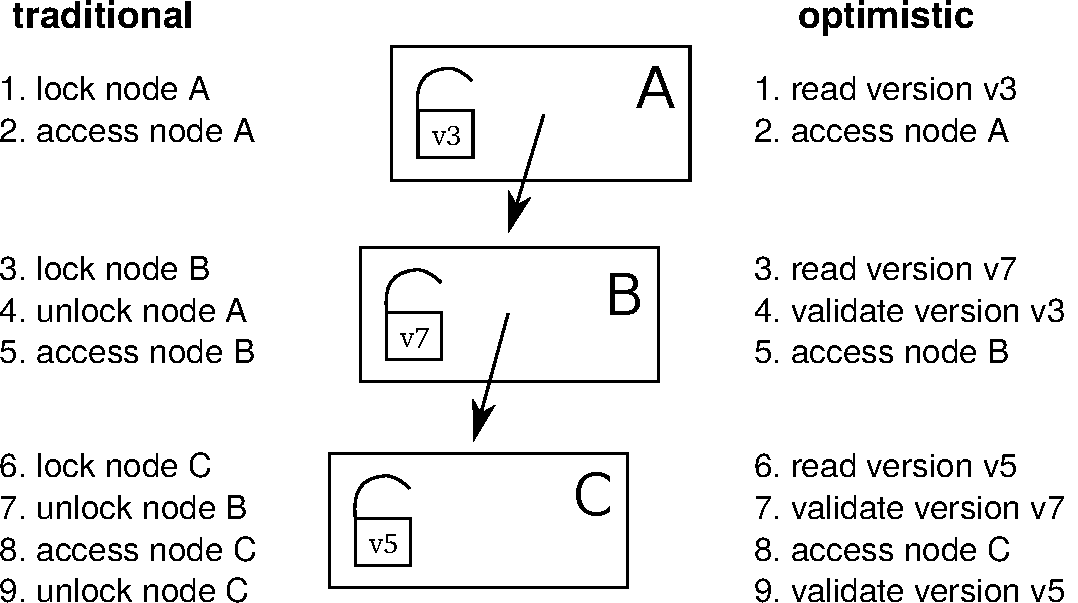
\includegraphics[width=0.65\linewidth]{olcall.pdf}
  \vspace{0.2cm}
  \caption{Comparison of a lookup operation in a 3-level tree using traditional lock coupling (left-hand side) vs.~optimistic lock coupling (right-hand side).}
  \label{fig:olc}
\end{figure}

The traditional and most common lock-based synchronization protocol for B-trees is lock coupling, which interleaves lock acquisitions while holding at most two locks at a time.
If, as we observed earlier, optimistic locks have similar semantics as traditional locks, it is natural to ask whether lock coupling can be combined with optimistic locks.
And indeed the answer is yes: One can almost mechanically translate traditional lock coupling code to optimistic lock coupling code.
This is illustrated in Figure~\ref{fig:olc}, which compares the traversal in a tree of height 3 using traditional and optimistic locks.
As the figure shows, the main difference is that locking is translated to reading the version and that unlocking becomes validation of the previously read version.
This simple change provides efficient lock-free tree traversal without the need to design a complex synchronization protocol.

It is important to emphasize the conceptual simplicity of OLC in comparison to data structures that use custom protocols like the Bw-tree~\cite{DBLP:conf/icde/LevandoskiLS13a}.
To implement lock-free access, the Bw-tree requires an indirection table, delta nodes, complex splitting and merging logic, retry logic, etc.
OLC, on the other hand, can directly be applied to B-trees mostly by adding the appropriate optimistic locking code and without modifying the node layout itself.
Therefore, OpenBw-Tree, an open source implementation of the Bw-tree, requires an order of magnitude more code than a B-tree based on OLC\footnote{Both implementations are available on GitHub: \url{https://github.com/wangziqi2016/index-microbench}}.
Given how difficult it is to develop, validate, and debug lock-free code, simplicity is obviously a major advantage.

\subsection{Correctness Aspects}

\begin{figure}
  % \centering
  %[basicstyle=\normalsize\ttfamily,showstringspaces=false,columns=fullflexible,breaklines=false,breakatwhitespace=true,numbers=none,numberstyle=\small,style=C,keepspaces=true]
\begin{lstlisting}[basicstyle=\ttfamily,language=C++,numbers=left,numberstyle=\small]
std::atomic<BTreeNode*> root;

// search for key in B+tree, returns payload in resultOut
bool lookup(Key key, Value& resultOut) {
   BTreeNode* node = root.load();
   uint64_t nodeVersion = node->readLockOrRestart();
   if (node != root.load()) // make sure the root is still the root
      restart();

   BTreeInner<Key>* parent = nullptr;
   uint64_t parentVersion = 0;

   while (node->isInner()) {
      auto inner = (BTreeInner*)node;

      // unlock parent and make current node the parent
      if (parent)
         parent->readUnlockOrRestart(parentVersion);
      parent = inner;
      parentVersion = nodeVersion;

      // search for next node
      node = inner->findChild(key);
      // validate 'inner' to ensure that 'node' pointer is valid
      inner->checkOrRestart(nodeVersion);
      // now it safe to dereference 'node' pointer (read its version)
      nodeVersion = node->readLockOrRestart();
   }

   // search in leaf and retrieve payload
   auto leaf = (BTreeLeaf*)node;
   bool success = leaf->findValue(key, resultOut);

   // unlock everything
   if (parent)
      parent->readUnlockOrRestart(parentVersion);
   node->readUnlockOrRestart(nodeVersion);

   return success;
}
\end{lstlisting}
  \vspace{0.2cm}
  \caption{B-tree lookup code using OLC. For simplicity, the restart logic is not shown.}
  \label{fig:lookup}
\end{figure}

So far, we have introduced the high-level ideas behind OLC and have stressed its similarity to traditional lock coupling.
Let us now discuss some cases where the close similarity between lock coupling and OLC breaks down.
To make this more concrete, we show the B-tree lookup code in Figure~\ref{fig:lookup}.
In the code, \texttt{readLockOrRestart} reads the lock version and \texttt{readUnlockOrRestart} validates that the read was correct.

One issue with OLC is that any pointer speculatively read from a node may point to invalid memory (if that node is modified concurrently).
Dereferencing such a pointer (e.g., to read its optimistic lock), may cause a segmentation fault or undefined behavior.
In the code shown in Figure~\ref{fig:lookup}, this problem is prevented by the extra check in line 25, which ensures that the read from the node containing the pointer was correct.
Without this additional validation, the code would in line 27 dereference the pointer speculatively read in line 23.
Note that the implementation of \texttt{checkOrRestart} is actually identical to \texttt{readUnlockOrRestart}.
We chose to give it a different name to highlight the fact that this extra check would not be necessary with read/write locks.

Another potential issue with optimistic locks is code that does not terminate.
Code that speculatively accesses a node, like an intra-node binary search, should be written in a way such that it always terminates---even in the presence of concurrent writes.
Otherwise, the validation code that detects the concurrent write will never run.
The binary search of a B-tree, for example, needs to be written in such a way that each comparison makes progress.
For some data structures that do not require loops in the traversal code (like ART) termination is trivially true.

\subsection{Implementation Details}

% implementation, efficiency
To implement an optimistic lock, one can combine the lock and the version counter into a single 64-bit\footnote{Even after subtracting one bit for the lock status, a back-of-the-envelope calculation can show that 63 bits are large enough to never overflow in practice.} word~\cite{artsync}.
A typical read operation will therefore merely consist of reading this version counter atomically.
In C++11 this can be implemented using the \texttt{std::atomic} type.

On x86, atomic reads are cheap because of x86's strong memory order guarantees.
No memory fences are required for sequentially-consistent loads, which are translated (by both GCC and clang) into standard \texttt{MOV} instructions.
Hence, the only effect of \texttt{std::atomic} for loads is preventing instruction re-ordering.
This makes version access and validation cheap.
Acquiring and releasing an optimistic lock in exclusive mode has comparable cost to a traditional lock:
A fairly expensive sequentially-consistent store is needed for acquiring a lock, while a standard \texttt{MOV} suffices for releasing it.
A simple sinlock-based implementation of optimistic locks can be found in the appendix of an earlier paper~\cite{artsync}.

OLC code must be able to handle restarts since validation or lock upgrade can fail due to concurrent writers.
Restarts can easily be implemented by wrapping the data structure operation in a loop (for simplicity not shown in Figure~\ref{fig:lookup}).
Such a loop also enables limiting the number of optimistic retry operations and falling back to pessimistic locking in cases of very heavy contention.
The ability to fall back to traditional locking is a major advantage of OLC in terms of robustness over lock-free approaches, which do not have this option.

In addition to the optimistic shared mode and the exclusive mode, optimistic locks also support a ``shared pessimistic'' mode, which physically acquires the lock in shared mode (allowing multiple concurrent readers but no writers).
This mode is useful for table (or range) scans that touch many tuples on a leaf page (which would otherwise easily abort).
Finally, let us mention that large range scans and table scans, should be broken up into several per-node traversals as is done in the LeanStore~\cite{leanstore} system.

Like all lock-free data structures, but unlike traditional locking and Hardware Transactional Memory~\cite{DBLP:conf/hpca/KarnagelDRLLSL14,DBLP:journals/pvldb/MakreshanskiLS15,htmtkde}, OLC requires care when deleting (and reusing) nodes.
The reason is that a deleting thread can never be sure that a node can be reclaimed because other threads might still be optimistically reading from that node.
Therefore, standard solutions like epoch-based reclamation~\cite{DBLP:conf/sosp/TuZKLM13}, hazard pointers~\cite{DBLP:journals/tpds/Michael04}, or optimized hazard pointers~\cite{DBLP:conf/spaa/BalmauGHZ16} need to be used.
These memory reclamation techniques are, however, largely orthogonal to the synchronization protocol itself.

%-lock-free is not a strong guarantee

\newpage
\section{Evaluation}\label{sec:evaluation}

Let us now experimentally evaluate the overhead and scalability of OLC.
For the experiments, we use an in-memory B+tree implemented in C++11 using templates, which is configured to use nodes of 4096 bytes, random 8 byte keys, and 8 byte payloads.
Based on this B-tree, we compare the following synchronization approaches:
\begin{itemize}
\item an OLC implementation\footnote{An almost identical OLC implementation is available on github: \url{https://github.com/wangziqi2016/index-microbench/tree/master/BTreeOLC}}
\item a variant based on traditional lock coupling and read/write locks
\item the unsynchronized B-tree, which obviously is only correct for read-only workloads but allows measuring the overhead of synchronization
\end{itemize}
Note that earlier work has compared the OLC implementation with a Bw-tree implementation~\cite{buzzword} and other state-of-the-art in-memory index structures.

We use a Haswell EP system with an Intel Xeon E5-2687W v3 CPU, which has 10 cores (20 ``Hyper-Threads'') and 25~MB of L3 cache.
The system is running Ubuntu 18.10 and we use GCC 8.2.0 to compile our code.
The CPU counters are obtained using the Linux perf API\footnote{We use the following convenience wrapper: \url{https://github.com/viktorleis/perfevent}}.

\begin{table}
  \caption{Performance and CPU counters for lookup and insert operations in a B-tree with 100M keys. We perform 100M operations and normalize the CPU counters by that number.}
  \label{tab:overhead}
  \centering
  \begin{tabular}{lrrrrrrr}\toprule
                    &         &        &        & instruc-  & L1     & L3     & branch \\
                    & threads & M op/s & cycles & tions & misses & misses & misses \\\midrule
lookup (no sync.)   & 1       & 1.72   & 2028   & 283     & 39.1   & 14.9   & 16.1   \\
lookup (OLC)        & 1       & 1.65   & 2107   & 370     & 43.9   & 15.1   & 16.7   \\
lookup (lock coup.) & 1       & 1.72   & 2078   & 365     & 42.3   & 16.9   & 15.7   \\\midrule
insert (no sync.)   & 1       & 1.51   & 2286   & 530     & 59.8   & 31.1   & 17.3   \\
insert (OLC)        & 1       & 1.50   & 2303   & 629     & 61.2   & 31.1   & 16.5   \\
insert (lock coup.) & 1       & 1.41   & 2473   & 644     & 61.0   & 31.0   & 17.2   \\\midrule
lookup (no sync.)   & 10      & 15.48  & 2058   & 283     & 38.6   & 15.5   & 16.0   \\
lookup (OLC)        & 10      & 14.60  & 2187   & 370     & 43.8   & 15.8   & 16.8   \\
lookup (lock coup.) & 10      & 5.71   & 5591   & 379     & 54.2   & 17.0   & 14.8   \\\midrule
insert (no sync.)   & 10      & -      & -      & -       & -      & -      & -      \\
insert (OLC)        & 10      & 10.46  & 2940   & 656     & 62.0   & 32.5   & 16.8   \\
insert (lock coup.) & 10      & 7.55   & 4161   & 667     & 75.0   & 28.6   & 16.2   \\
    \bottomrule
\end{tabular}
\end{table}

Table~\ref{tab:overhead} compares the performance and CPU counters for lookup and insert operations in a B-tree with 100M keys.
With {\em single-threaded} execution, we observe that all three approaches have very similar performance.
Adding traditional or optimistic locks to unsynchronized B-tree code results in up to 30\% of additional instructions without affecting single-threaded performance much.

\begin{figure}
  \centering
  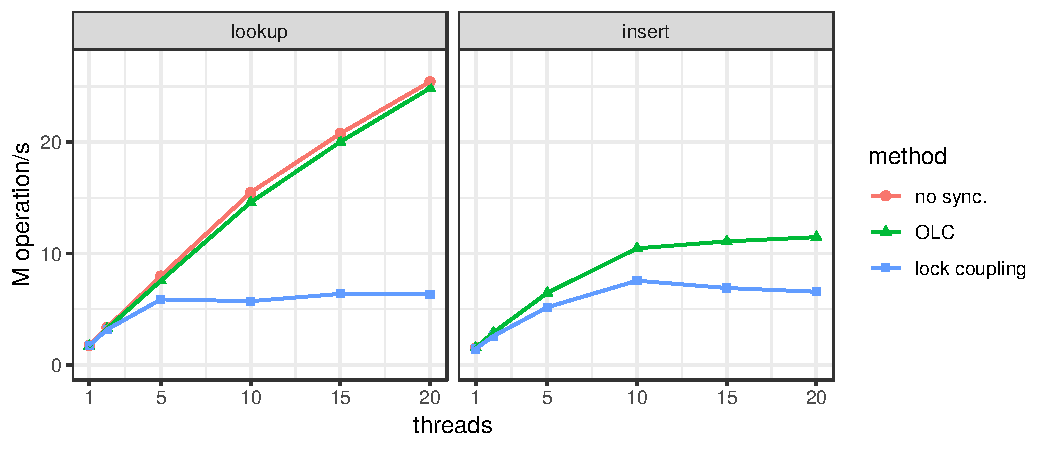
\includegraphics[width=\linewidth]{scale.pdf}
  \vspace{0.2cm}
  \caption{Scalability on 10-core system for B-tree operations (100M values).}
  \label{fig:scale}
\end{figure}

As Figure~\ref{fig:scale} shows, the results change dramatically once we use multiple threads.
For lookup, the scalability of OLC is near-linear up to 20 threads, even though the system has only 10 ``real cores''.
The OLC scalability for insert is also respectable (though not quite as linear because multi-threaded insertion approaches the memory bandwidth of our processor).
The figure also shows that the results of traditional lock coupling with read/write locks are significantly worse than OLC.
With 20 threads, lookup with OLC is 3.9$\times$ faster than traditional lock coupling.

\section{Summary}\label{sec:conc}

Optimistic Lock Coupling (OLC) is an effective synchronization method that combines the simplicity of traditional lock coupling with the superior scalability of lock-free approaches.
OLC is widely applicable and has already been successfully used to synchronize several data structures, including B-trees, binary search trees, and different trie variants.
These features make it highly attractive for modern database systems as well as performance-critical systems software in general.

\begin{thebibliography}{10}

\bibitem{DBLP:conf/spaa/BalmauGHZ16}
O.~Balmau, R.~Guerraoui, M.~Herlihy, and I.~Zablotchi.
\newblock Fast and robust memory reclamation for concurrent data structures.
\newblock In {\em SPAA}, 2016.

\bibitem{DBLP:journals/acta/BayerS77}
R.~Bayer and M.~Schkolnick.
\newblock Concurrency of operations on {B}-trees.
\newblock {\em Acta Informatica}, 9, 1977.

\bibitem{hot}
R.~Binna, E.~Zangerle, M.~Pichl, G.~Specht, and V.~Leis.
\newblock {HOT}: A height optimized trie index for main-memory database
  systems.
\newblock In {\em SIGMOD}, 2018.

\bibitem{DBLP:conf/ppopp/BronsonCCO10}
N.~G. Bronson, J.~Casper, H.~Chafi, and K.~Olukotun.
\newblock A practical concurrent binary search tree.
\newblock In {\em PPOPP}, 2010.

\bibitem{DBLP:conf/vldb/ChaHKK01}
S.~K. Cha, S.~Hwang, K.~Kim, and K.~Kwon.
\newblock Cache-conscious concurrency control of main-memory indexes on
  shared-memory multiprocessor systems.
\newblock In {\em VLDB}, 2001.

\bibitem{intel}
I.~Cutress.
\newblock {Intel} goes for 48-cores: {Cascade-AP} with multi-chip package
  coming soon.
\newblock
  \url{https://www.anandtech.com/show/13535/intel-goes-for-48cores-cascade-ap},
  2018 (accessed January, 2019).

\bibitem{DBLP:conf/cidr/FaleiroA17}
J.~M. Faleiro and D.~J. Abadi.
\newblock Latch-free synchronization in database systems: Silver bullet or
  fool's gold?
\newblock In {\em CIDR}, 2017.

\bibitem{DBLP:journals/ftdb/Graefe11}
G.~Graefe.
\newblock Modern {B}-tree techniques.
\newblock {\em Foundations and Trends in Databases}, 3(4), 2011.

\bibitem{DBLP:conf/hpca/KarnagelDRLLSL14}
T.~Karnagel, R.~Dementiev, R.~Rajwar, K.~Lai, T.~Legler, B.~Schlegel, and
  W.~Lehner.
\newblock Improving in-memory database index performance with
  {Intel}\({}^{\mbox{{\textregistered}}}\) transactional synchronization
  extensions.
\newblock In {\em HPCA}, 2014.

\bibitem{DBLP:journals/tods/LehmanY81}
P.~L. Lehman and S.~B. Yao.
\newblock Efficient locking for concurrent operations on {B}-trees.
\newblock {\em {ACM} Trans. Database Syst.}, 6(4), 1981.

\bibitem{leanstore}
V.~Leis, M.~Haubenschild, A.~Kemper, and T.~Neumann.
\newblock Leanstore: In-memory data management beyond main memory.
\newblock In {\em ICDE}, 2018.

\bibitem{art}
V.~Leis, A.~Kemper, and T.~Neumann.
\newblock The adaptive radix tree: {ARTful} indexing for main-memory databases.
\newblock In {\em ICDE}, 2013.

\bibitem{htmtkde}
V.~Leis, A.~Kemper, and T.~Neumann.
\newblock Scaling {HTM}-supported database transactions to many cores.
\newblock {\em {IEEE} Trans. Knowl. Data Eng.}, 28(2), 2016.

\bibitem{artsync}
V.~Leis, F.~Scheibner, A.~Kemper, and T.~Neumann.
\newblock The {ART} of practical synchronization.
\newblock In {\em DaMoN}, 2016.

\bibitem{DBLP:conf/icde/LevandoskiLS13a}
J.~J. Levandoski, D.~B. Lomet, and S.~Sengupta.
\newblock The {Bw}-tree: A {B}-tree for new hardware platforms.
\newblock In {\em ICDE}, 2013.

\bibitem{DBLP:journals/pvldb/MakreshanskiLS15}
D.~Makreshanski, J.~J. Levandoski, and R.~Stutsman.
\newblock To lock, swap, or elide: On the interplay of hardware transactional
  memory and lock-free indexing.
\newblock {\em {PVLDB}}, 8(11), 2015.

\bibitem{DBLP:dblp_conf/eurosys/MaoKM12}
Y.~Mao, E.~Kohler, and R.~T. Morris.
\newblock Cache craftiness for fast multicore key-value storage.
\newblock In {\em EuroSys}, 2012.

\bibitem{DBLP:journals/tpds/Michael04}
M.~M. Michael.
\newblock Hazard pointers: Safe memory reclamation for lock-free objects.
\newblock {\em {IEEE} Trans. Parallel Distrib. Syst.}, 15(6), 2004.

\bibitem{DBLP:journals/jacm/ShalevS06}
O.~Shalev and N.~Shavit.
\newblock Split-ordered lists: Lock-free extensible hash tables.
\newblock {\em J. {ACM}}, 53(3), 2006.

\bibitem{amd}
A.~Shilov.
\newblock {AMD} previews {EPYC} ‘{Rome}’ processor: Up to 64 {Zen} 2 cores.
\newblock
  \url{https://www.anandtech.com/show/13561/amd-previews-epyc-rome-processor-up-to-64-zen-2-cores},
  2018 (accessed January, 2019).

\bibitem{DBLP:conf/sosp/TuZKLM13}
S.~Tu, W.~Zheng, E.~Kohler, B.~Liskov, and S.~Madden.
\newblock Speedy transactions in multicore in-memory databases.
\newblock In {\em SOSP}, 2013.

\bibitem{buzzword}
Z.~Wang, A.~Pavlo, H.~Lim, V.~Leis, H.~Zhang, M.~Kaminsky, and D.~Andersen.
\newblock Building a {Bw}-tree takes more than just buzz words.
\newblock In {\em SIGMOD}, 2018.

\end{thebibliography}


%\bibliographystyle{abbrv}
%\bibliography{main}

\end{document}

\end{article}

\begin{article}
{Quill: A Declarative Approach for Accelerating Augmented Reality Application Development}
{Codi Burley, Ritesh Sarkhel, and Arnab Nandi}
\pdfminorversion=5
\documentclass[11pt]{article}
\usepackage{deauthor,times,graphicx,caption,microtype}
\usepackage{hyperref}
\usepackage{listings}
\usepackage{booktabs}

\begin{document}

\title{Optimistic Lock Coupling: A Scalable and Efficient General-Purpose Synchronization Method}

\author{Viktor Leis, Michael Haubenschild\raisebox{0.9ex}{$\ast$}, Thomas Neumann\\ Technische Universit{\"a}t M{\"u}nchen \hspace{0.7cm} Tableau Software\raisebox{0.9ex}{$\ast$} \\ {\{leis,neumann\}{@}in.tum.de} \hspace{0.7cm} {mhaubenschild{@}tableau.com\raisebox{0.9ex}{$\ast$}}}

\maketitle

\begin{abstract}
As the number of cores on commodity processors continues to increase, scalability becomes more and more crucial for overall performance.
Scalable and efficient concurrent data structures are particularly important, as these are often the building blocks of parallel algorithms.
Unfortunately, traditional synchronization techniques based on fine-grained locking have been shown to be unscalable on modern multi-core CPUs.
Lock-free data structures, on the other hand, are extremely difficult to design and often incur significant overhead.

In this work, we make the case for Optimistic Lock Coupling as a practical alternative to both traditional locking and the lock-free approach.
We show that Optimistic Lock Coupling is highly scalable and almost as simple to implement as traditional lock coupling.
Another important advantage is that it is easily applicable to most tree-like data structures.
We therefore argue that Optimistic Lock Coupling, rather than a complex and error-prone custom synchronization protocol, should be the default choice for performance-critical data structures.
\end{abstract}

\section{Introduction}

% more and more cores
Today, Intel's commodity server processors have up to 28 cores and its upcoming microarchitecture will have up to 48 cores per socket~\cite{intel}.
Similarly, AMD currently stands at 32 cores and this number is expected to double in the next generation~\cite{amd}.
Since both platforms support simultaneous multithreading (also known as hyperthreading), affordable commodity servers (with up to two sockets) will soon routinely have between 100 and 200 hardware threads.

% data structure scalability is important
With such a high degree of hardware parallelism, efficient data processing crucially depends on how well concurrent data structures scale.
Internally, database systems use a plethora of data structures like table heaps, internal work queues, and, most importantly, index structures.
Any of these can easily become a scalability (and therefore overall performance) bottleneck on many-core CPUs.

% traditional synchronization: fine-grained locks, slow, cache invalidation
Traditionally, database systems synchronize internal data structures using fine-grained reader/writer locks\footnote{In this work, we focus on data structure synchronization rather than high-level transaction semantics and therefore use the term {\em lock} for what would typically be called {\em latch} in the database literature. We thus follow common computer science (rather than database) terminology.}.
Unfortunately, while fine-grained locking makes lock contention unlikely, it still results in bad scalability because lock acquisition and release require writing to shared memory.
Due to the way cache coherency is implemented on modern multi-core CPUs, these writes cause additional cache misses\footnote{The cache coherency protocol ensures that all copies of a cache line on other cores are invalidated before the write can proceed.} and the cache line containing the lock's internal data becomes a point of physical contention.
As a result, any frequently-accessed lock (e.g., the lock of the root node of a B-tree) severely limits scalability.

% lock-free bw-tree: no more latches, but indirections, extremely complex
Lock-free data structures like the Bw-tree~\cite{DBLP:conf/icde/LevandoskiLS13a} (a lock-free B-tree variant) or the Split-Ordered List~\cite{DBLP:journals/jacm/ShalevS06} (a lock-free hash table) do not acquire any locks and therefore generally scale much better than locking-based approaches (in particular for read-mostly workloads).
However, lock-free synchronization has other downsides:
First, it is very difficult and results in extremely complex and error-prone code (when compared to locking).
Second, because the functionality of atomic primitives provided by the hardware (e.g., atomically compare-and-swap 8 bytes) is limited, complex operations require additional indirections within the data structure.
For example, the Bw-tree requires an indirection table and the Split-Ordered List requires ``dummy nodes'', resulting in overhead due to additional cache misses.

% OLC for the win
In this paper we make the case for {\em Optimistic Lock Coupling (OLC)}, a synchronization method that combines some of the best properties of lock-based and lock-free synchronization.
OLC utilizes a special lock type that can be used in two modes:
The first mode is similar to a traditional mutex and excludes other threads by physically acquiring the underlying lock.
In the second mode, reads can proceed optimistically by validating a version counter that is embedded in the lock (similar to optimistic concurrency control).
The first mode is typically used by writers and the second mode by readers.
Besides this special lock type, OLC is based on the observation that optimistic lock validations can be interleaved/coupled---similar to the pair-wise interleaved lock acquisition of traditional lock coupling.
Hence, the name Optimistic Lock Coupling.

OLC has a number of desirable features:
\begin{itemize}
\item By reducing the number of writes to shared memory locations and thereby avoiding cache invalidations, it {\bf scales well} for most workloads.
\item In comparison to unsynchronized code, it requires few additional CPU instructions making it {\bf efficient}.
\item OLC is {\bf widely applicable} to different data structures. It has already been successfully used for synchronizing binary search trees~\cite{DBLP:conf/ppopp/BronsonCCO10}, tries~\cite{artsync}, trie/B-tree hybrids~\cite{DBLP:dblp_conf/eurosys/MaoKM12}, and B-trees~\cite{buzzword}.
\item In comparison to the lock-free paradigm, it is also {\bf easy to use} and requires few modifications to existing, single-threaded data structures.
\end{itemize}
Despite these positive features and its simplicity, OLC is not yet widely known.
The goal of this paper is therefore to popularize this simple idea and to make a case for it.
We argue that OLC deserves to be widely known.
It is a good default synchronization paradigm---more complex, data structure-specific protocols are seldom beneficial.

The rest of the paper is organized as follows.
Section~\ref{sec:related} discusses related work, tracing the history of OLC and its underlying ideas in the literature.
The core of the paper is Section~\ref{sec:olc}, which describes the ideas behind OLC and how it can be used to synchronize complex data structures.
In Section~\ref{sec:evaluation} we experimentally show that OLC has low overhead and scales well when used to synchronize an in-memory B-tree.
We summarize the paper in Section~\ref{sec:conc}.

\newpage
\section{Related Work}\label{sec:related}

Lock coupling has been proposed as a method for allowing concurrent operations on B-trees in 1977~\cite{DBLP:journals/acta/BayerS77}.
This traditional and still widely-used method, described in detail in Graefe's B-tree survey~\cite{DBLP:journals/ftdb/Graefe11}, is also called ``latch coupling'', ``hand-over-hand locking'', and ``crabbing''.
Because at most two locks are held at-a-time during tree traversal, this technique seemingly allows for a high degree of parallelism---in particular if read/write locks are used to enable inner nodes to be locked in shared mode.
However, as we show in Section~\ref{sec:evaluation}, on modern hardware lock acquisition (even in shared mode) results in suboptimal scalability.

An early alternative from 1981 is a B-tree variant called B-link tree~\cite{DBLP:journals/tods/LehmanY81}, which only holds a single lock at a time.
It is based on the observation that between the release of the parent lock and the acquisition of the child lock, the only ``dangerous'' thing that could have happened is the split of a child node (assuming one does not implement merge operations).
Thus, when a split happens, the key being searched might end up on a neighboring node to the right of the current child node.
A B-link tree traversal therefore detects this condition and, if needed, transparently proceeds to the neighboring node.
Releasing the parent lock early is highly beneficial when the child node needs to be fetched from disk.
For in-memory workloads, however, the B-link tree has the same scalability issues as lock coupling (it acquires just as many locks).

The next major advance, Optimistic Latch-Free Index Traversal (OLFIT)~\cite{DBLP:conf/vldb/ChaHKK01}, was proposed in 2001.
OLFIT introduced the idea of a combined lock/update counter, which we call {\em optimistic lock}. % , for lack of a better name,
Based on these per-node optimistic locks and the synchronization protocol of the B-link tree, OLFIT finally achieves good scalability on parallel processors.
The OLFIT protocol is fairly complex, as it requires both the non-trivial B-link protocol and optimistic locks.
Furthermore, like the B-link tree protocol, it does not support merging nodes, and is specific to B-trees (cannot easily be applied to other data structures).

In the following two decades, the growth of main-memory capacity led to much research into other data structures besides the venerable B-tree.
Particularly relevant for our discussion is Bronson et al.'s~\cite{DBLP:conf/ppopp/BronsonCCO10} concurrent binary search tree, which is based on optimistic version validation and has a sophisticated, data structure-specific synchronization protocol.
To the best of our knowledge, this 2010 paper is the first that, as part of its protocol, interleaves version validation across nodes---rather than validating each node separately like OLFIT.
In that paper, this idea is called ``hand-over-hand, optimistic validation'', while we prefer the term Optimistic Lock Coupling to highlight the close resemblance to traditional lock coupling.
Similarly, Mao et al.'s~\cite{DBLP:dblp_conf/eurosys/MaoKM12} Masstree (a concurrent hybrid trie/B-tree) is also based on the same ideas, but again uses them as part of a more complex protocol.

The Adaptive Radix Tree (ART)~\cite{art} is another recent in-memory data structure, which we proposed in 2013.
In contrast to the two data structures just mentioned, it was originally designed with single-threaded performance in mind without supporting concurrency.
To add support for concurrency, we initially started designing a custom protocol called Read-Optimized Write Exclusion (ROWEX)~\cite{artsync}, which turned out to be non-trivial and requires modifications of the underlying data structure\footnote{Note that ROWEX is already easier to apply to existing data structures than the lock-free approach. The difficulty depends on the data structure. Applying ROWEX is hard for B-trees with sorted keys and fairly easy for copy-on-write data structures like the Height Optimized Trie~\cite{hot}---with ART being somewhere in the middle.}.
However, fairly late in the project, we also realized, that OLC {\em alone} (rather than as part of a more complex protocol) is sufficient to synchronize ART.
No other changes to the data structure were necessary.
Both approaches were published and experimentally evaluated in a followup paper~\cite{artsync}, which shows that, despite its simplicity, OLC is efficient, scalable, and generally outperforms ROWEX.

Similar results were recently published regarding B-trees~\cite{buzzword}.
In this experimental study a simple OLC-based synchronization outperformed the Bw-tree~\cite{DBLP:conf/icde/LevandoskiLS13a}, a complex lock-free synchronization approach.
Another recent paper shows that for write-intensive workloads, locking often performs better than lock-free synchronization~\cite{DBLP:conf/cidr/FaleiroA17}.
These experiences indicate that OLC is a general-purpose synchronization paradigm and motivate the current paper.

%foster b-tree\cite{DBLP:journals/tods/GraefeKK12}
%Shasha theory~\cite{DBLP:journals/tods/ShashaG88}

\section{Optimistic Lock Coupling}\label{sec:olc}

% locks suck
The standard technique for inter-thread synchronization is mutual exclusion using fine-grained locks.
In a B-tree, for example, every node usually has its own associated lock, which is acquired before accessing that node.
The problem of locking on modern multi- and many-core processors is that lock acquisition and release require writing to the shared memory location that implements the lock.
This write causes exclusive ownership of the underlying cache line and invalidates copies of it on all other processor cores.
For hierarchical, tree-like data structures, the lock of the root node becomes a point of physical contention---even in read-only workloads and even when read/write locks are used.
Depending on the specific data structure, number of cores, cache coherency protocol implementation, cache topology, whether Non-Uniform Memory Access (NUMA) is used, locking can even result in multi-threaded performance that is worse than single-threaded execution.

% in b-trees this happens very much
The inherent pessimism of locking is particularly unfortunate for B-trees:
Despite the fact that logical modifications of the root node are very infrequent, every B-tree operation must lock the root node during tree traversal\footnote{To a lesser extent this obviously applies to all inner nodes, not just the root.}.
Even the vast majority of update operations (with the exception of splits and merges), only modify a single leaf node.
These observations indicate that a more optimistic approach, which does not require locking inner nodes, would be very beneficial for B-trees.

\subsection{Optimistic Locks}

% optimism to the rescue
As the name indicates, optimistic locks try to solve the scalability issues of traditional locks using an optimistic approach.
Instead of always physically acquiring locks, even for nodes that are unlikely to be modified simultaneously, after-the-fact validation is used to detect conflicts.
This is done by augmenting each lock with a version/update counter that is incremented on every modification.
Using this version counter, readers can optimistically proceed before validating that the version did not change to ensure that the read was safe.
If validation fails, the operation is restarted.

% details on opt locks
Using optimistic locks, a read-only node access (i.e., the majority of all operations in a B-tree) does not acquire the lock and does not increment the version counter.
Instead, it performs the following steps:
\begin{enumerate}
\item read lock version (restart if lock is not free)
\item access node
\item read the version again and validate that it has not changed in the meantime
\end{enumerate}
If the last step (the validation) fails, the operation has to be restarted.
Write operations, on the other hand, are more similar to traditional locking:
\begin{enumerate}
\item acquire lock (wait if necessary)
\item access/write to node
\item increment version and unlock node
\end{enumerate}
Writes can therefore protect a node from other writes.

% similar to locks
As we observed in an earlier paper~\cite{artsync}, because of similar semantics, optimistic locks can be hidden behind an API very similar to traditional read/write locks.
Both approaches have an exclusive lock mode, and acquiring a traditional lock in shared mode is analogous to optimistic version validation.
Furthermore, like with some implementations of traditional read/write locks, optimistic locks allow upgrading a shared lock to an exclusive lock.
Lock upgrades are, for example, used to avoid most B-tree update operations from having to lock inner nodes.
In our experience, the close resemblance of optimistic and traditional locks simplifies the reasoning about optimistic locks;
one can apply similar thinking as in traditional lock-based protocols.

\subsection{Lock Coupling with Optimistic Locks}

\begin{figure}
  \centering
  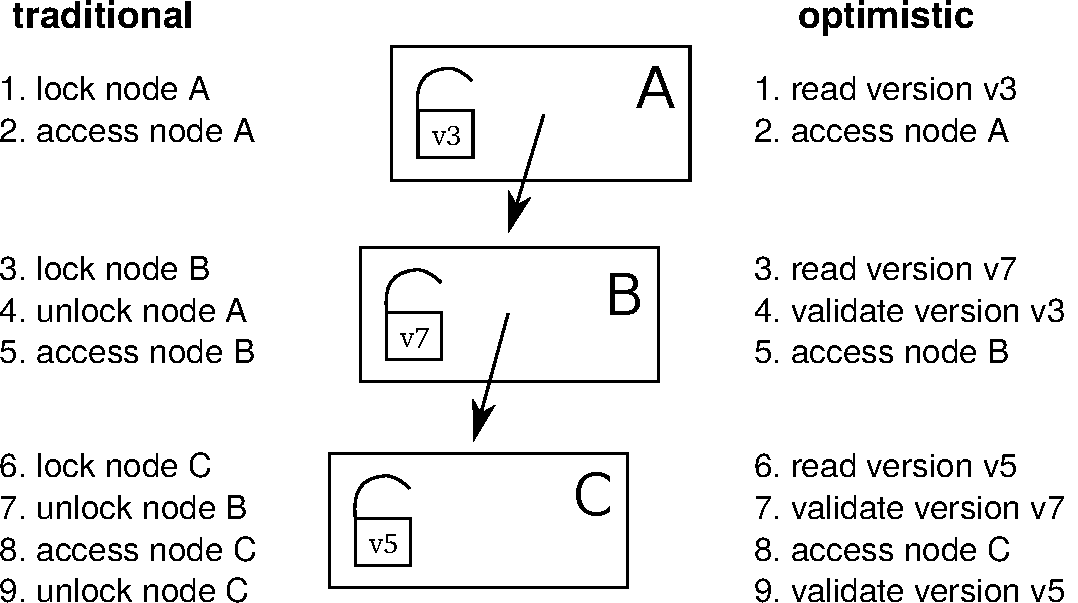
\includegraphics[width=0.65\linewidth]{olcall.pdf}
  \vspace{0.2cm}
  \caption{Comparison of a lookup operation in a 3-level tree using traditional lock coupling (left-hand side) vs.~optimistic lock coupling (right-hand side).}
  \label{fig:olc}
\end{figure}

The traditional and most common lock-based synchronization protocol for B-trees is lock coupling, which interleaves lock acquisitions while holding at most two locks at a time.
If, as we observed earlier, optimistic locks have similar semantics as traditional locks, it is natural to ask whether lock coupling can be combined with optimistic locks.
And indeed the answer is yes: One can almost mechanically translate traditional lock coupling code to optimistic lock coupling code.
This is illustrated in Figure~\ref{fig:olc}, which compares the traversal in a tree of height 3 using traditional and optimistic locks.
As the figure shows, the main difference is that locking is translated to reading the version and that unlocking becomes validation of the previously read version.
This simple change provides efficient lock-free tree traversal without the need to design a complex synchronization protocol.

It is important to emphasize the conceptual simplicity of OLC in comparison to data structures that use custom protocols like the Bw-tree~\cite{DBLP:conf/icde/LevandoskiLS13a}.
To implement lock-free access, the Bw-tree requires an indirection table, delta nodes, complex splitting and merging logic, retry logic, etc.
OLC, on the other hand, can directly be applied to B-trees mostly by adding the appropriate optimistic locking code and without modifying the node layout itself.
Therefore, OpenBw-Tree, an open source implementation of the Bw-tree, requires an order of magnitude more code than a B-tree based on OLC\footnote{Both implementations are available on GitHub: \url{https://github.com/wangziqi2016/index-microbench}}.
Given how difficult it is to develop, validate, and debug lock-free code, simplicity is obviously a major advantage.

\subsection{Correctness Aspects}

\begin{figure}
  % \centering
  %[basicstyle=\normalsize\ttfamily,showstringspaces=false,columns=fullflexible,breaklines=false,breakatwhitespace=true,numbers=none,numberstyle=\small,style=C,keepspaces=true]
\begin{lstlisting}[basicstyle=\ttfamily,language=C++,numbers=left,numberstyle=\small]
std::atomic<BTreeNode*> root;

// search for key in B+tree, returns payload in resultOut
bool lookup(Key key, Value& resultOut) {
   BTreeNode* node = root.load();
   uint64_t nodeVersion = node->readLockOrRestart();
   if (node != root.load()) // make sure the root is still the root
      restart();

   BTreeInner<Key>* parent = nullptr;
   uint64_t parentVersion = 0;

   while (node->isInner()) {
      auto inner = (BTreeInner*)node;

      // unlock parent and make current node the parent
      if (parent)
         parent->readUnlockOrRestart(parentVersion);
      parent = inner;
      parentVersion = nodeVersion;

      // search for next node
      node = inner->findChild(key);
      // validate 'inner' to ensure that 'node' pointer is valid
      inner->checkOrRestart(nodeVersion);
      // now it safe to dereference 'node' pointer (read its version)
      nodeVersion = node->readLockOrRestart();
   }

   // search in leaf and retrieve payload
   auto leaf = (BTreeLeaf*)node;
   bool success = leaf->findValue(key, resultOut);

   // unlock everything
   if (parent)
      parent->readUnlockOrRestart(parentVersion);
   node->readUnlockOrRestart(nodeVersion);

   return success;
}
\end{lstlisting}
  \vspace{0.2cm}
  \caption{B-tree lookup code using OLC. For simplicity, the restart logic is not shown.}
  \label{fig:lookup}
\end{figure}

So far, we have introduced the high-level ideas behind OLC and have stressed its similarity to traditional lock coupling.
Let us now discuss some cases where the close similarity between lock coupling and OLC breaks down.
To make this more concrete, we show the B-tree lookup code in Figure~\ref{fig:lookup}.
In the code, \texttt{readLockOrRestart} reads the lock version and \texttt{readUnlockOrRestart} validates that the read was correct.

One issue with OLC is that any pointer speculatively read from a node may point to invalid memory (if that node is modified concurrently).
Dereferencing such a pointer (e.g., to read its optimistic lock), may cause a segmentation fault or undefined behavior.
In the code shown in Figure~\ref{fig:lookup}, this problem is prevented by the extra check in line 25, which ensures that the read from the node containing the pointer was correct.
Without this additional validation, the code would in line 27 dereference the pointer speculatively read in line 23.
Note that the implementation of \texttt{checkOrRestart} is actually identical to \texttt{readUnlockOrRestart}.
We chose to give it a different name to highlight the fact that this extra check would not be necessary with read/write locks.

Another potential issue with optimistic locks is code that does not terminate.
Code that speculatively accesses a node, like an intra-node binary search, should be written in a way such that it always terminates---even in the presence of concurrent writes.
Otherwise, the validation code that detects the concurrent write will never run.
The binary search of a B-tree, for example, needs to be written in such a way that each comparison makes progress.
For some data structures that do not require loops in the traversal code (like ART) termination is trivially true.

\subsection{Implementation Details}

% implementation, efficiency
To implement an optimistic lock, one can combine the lock and the version counter into a single 64-bit\footnote{Even after subtracting one bit for the lock status, a back-of-the-envelope calculation can show that 63 bits are large enough to never overflow in practice.} word~\cite{artsync}.
A typical read operation will therefore merely consist of reading this version counter atomically.
In C++11 this can be implemented using the \texttt{std::atomic} type.

On x86, atomic reads are cheap because of x86's strong memory order guarantees.
No memory fences are required for sequentially-consistent loads, which are translated (by both GCC and clang) into standard \texttt{MOV} instructions.
Hence, the only effect of \texttt{std::atomic} for loads is preventing instruction re-ordering.
This makes version access and validation cheap.
Acquiring and releasing an optimistic lock in exclusive mode has comparable cost to a traditional lock:
A fairly expensive sequentially-consistent store is needed for acquiring a lock, while a standard \texttt{MOV} suffices for releasing it.
A simple sinlock-based implementation of optimistic locks can be found in the appendix of an earlier paper~\cite{artsync}.

OLC code must be able to handle restarts since validation or lock upgrade can fail due to concurrent writers.
Restarts can easily be implemented by wrapping the data structure operation in a loop (for simplicity not shown in Figure~\ref{fig:lookup}).
Such a loop also enables limiting the number of optimistic retry operations and falling back to pessimistic locking in cases of very heavy contention.
The ability to fall back to traditional locking is a major advantage of OLC in terms of robustness over lock-free approaches, which do not have this option.

In addition to the optimistic shared mode and the exclusive mode, optimistic locks also support a ``shared pessimistic'' mode, which physically acquires the lock in shared mode (allowing multiple concurrent readers but no writers).
This mode is useful for table (or range) scans that touch many tuples on a leaf page (which would otherwise easily abort).
Finally, let us mention that large range scans and table scans, should be broken up into several per-node traversals as is done in the LeanStore~\cite{leanstore} system.

Like all lock-free data structures, but unlike traditional locking and Hardware Transactional Memory~\cite{DBLP:conf/hpca/KarnagelDRLLSL14,DBLP:journals/pvldb/MakreshanskiLS15,htmtkde}, OLC requires care when deleting (and reusing) nodes.
The reason is that a deleting thread can never be sure that a node can be reclaimed because other threads might still be optimistically reading from that node.
Therefore, standard solutions like epoch-based reclamation~\cite{DBLP:conf/sosp/TuZKLM13}, hazard pointers~\cite{DBLP:journals/tpds/Michael04}, or optimized hazard pointers~\cite{DBLP:conf/spaa/BalmauGHZ16} need to be used.
These memory reclamation techniques are, however, largely orthogonal to the synchronization protocol itself.

%-lock-free is not a strong guarantee

\newpage
\section{Evaluation}\label{sec:evaluation}

Let us now experimentally evaluate the overhead and scalability of OLC.
For the experiments, we use an in-memory B+tree implemented in C++11 using templates, which is configured to use nodes of 4096 bytes, random 8 byte keys, and 8 byte payloads.
Based on this B-tree, we compare the following synchronization approaches:
\begin{itemize}
\item an OLC implementation\footnote{An almost identical OLC implementation is available on github: \url{https://github.com/wangziqi2016/index-microbench/tree/master/BTreeOLC}}
\item a variant based on traditional lock coupling and read/write locks
\item the unsynchronized B-tree, which obviously is only correct for read-only workloads but allows measuring the overhead of synchronization
\end{itemize}
Note that earlier work has compared the OLC implementation with a Bw-tree implementation~\cite{buzzword} and other state-of-the-art in-memory index structures.

We use a Haswell EP system with an Intel Xeon E5-2687W v3 CPU, which has 10 cores (20 ``Hyper-Threads'') and 25~MB of L3 cache.
The system is running Ubuntu 18.10 and we use GCC 8.2.0 to compile our code.
The CPU counters are obtained using the Linux perf API\footnote{We use the following convenience wrapper: \url{https://github.com/viktorleis/perfevent}}.

\begin{table}
  \caption{Performance and CPU counters for lookup and insert operations in a B-tree with 100M keys. We perform 100M operations and normalize the CPU counters by that number.}
  \label{tab:overhead}
  \centering
  \begin{tabular}{lrrrrrrr}\toprule
                    &         &        &        & instruc-  & L1     & L3     & branch \\
                    & threads & M op/s & cycles & tions & misses & misses & misses \\\midrule
lookup (no sync.)   & 1       & 1.72   & 2028   & 283     & 39.1   & 14.9   & 16.1   \\
lookup (OLC)        & 1       & 1.65   & 2107   & 370     & 43.9   & 15.1   & 16.7   \\
lookup (lock coup.) & 1       & 1.72   & 2078   & 365     & 42.3   & 16.9   & 15.7   \\\midrule
insert (no sync.)   & 1       & 1.51   & 2286   & 530     & 59.8   & 31.1   & 17.3   \\
insert (OLC)        & 1       & 1.50   & 2303   & 629     & 61.2   & 31.1   & 16.5   \\
insert (lock coup.) & 1       & 1.41   & 2473   & 644     & 61.0   & 31.0   & 17.2   \\\midrule
lookup (no sync.)   & 10      & 15.48  & 2058   & 283     & 38.6   & 15.5   & 16.0   \\
lookup (OLC)        & 10      & 14.60  & 2187   & 370     & 43.8   & 15.8   & 16.8   \\
lookup (lock coup.) & 10      & 5.71   & 5591   & 379     & 54.2   & 17.0   & 14.8   \\\midrule
insert (no sync.)   & 10      & -      & -      & -       & -      & -      & -      \\
insert (OLC)        & 10      & 10.46  & 2940   & 656     & 62.0   & 32.5   & 16.8   \\
insert (lock coup.) & 10      & 7.55   & 4161   & 667     & 75.0   & 28.6   & 16.2   \\
    \bottomrule
\end{tabular}
\end{table}

Table~\ref{tab:overhead} compares the performance and CPU counters for lookup and insert operations in a B-tree with 100M keys.
With {\em single-threaded} execution, we observe that all three approaches have very similar performance.
Adding traditional or optimistic locks to unsynchronized B-tree code results in up to 30\% of additional instructions without affecting single-threaded performance much.

\begin{figure}
  \centering
  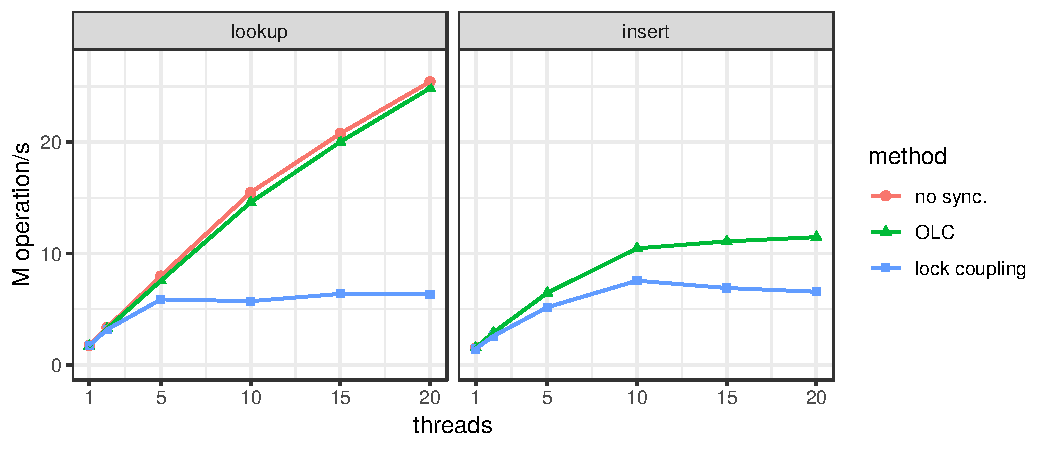
\includegraphics[width=\linewidth]{scale.pdf}
  \vspace{0.2cm}
  \caption{Scalability on 10-core system for B-tree operations (100M values).}
  \label{fig:scale}
\end{figure}

As Figure~\ref{fig:scale} shows, the results change dramatically once we use multiple threads.
For lookup, the scalability of OLC is near-linear up to 20 threads, even though the system has only 10 ``real cores''.
The OLC scalability for insert is also respectable (though not quite as linear because multi-threaded insertion approaches the memory bandwidth of our processor).
The figure also shows that the results of traditional lock coupling with read/write locks are significantly worse than OLC.
With 20 threads, lookup with OLC is 3.9$\times$ faster than traditional lock coupling.

\section{Summary}\label{sec:conc}

Optimistic Lock Coupling (OLC) is an effective synchronization method that combines the simplicity of traditional lock coupling with the superior scalability of lock-free approaches.
OLC is widely applicable and has already been successfully used to synchronize several data structures, including B-trees, binary search trees, and different trie variants.
These features make it highly attractive for modern database systems as well as performance-critical systems software in general.

\begin{thebibliography}{10}

\bibitem{DBLP:conf/spaa/BalmauGHZ16}
O.~Balmau, R.~Guerraoui, M.~Herlihy, and I.~Zablotchi.
\newblock Fast and robust memory reclamation for concurrent data structures.
\newblock In {\em SPAA}, 2016.

\bibitem{DBLP:journals/acta/BayerS77}
R.~Bayer and M.~Schkolnick.
\newblock Concurrency of operations on {B}-trees.
\newblock {\em Acta Informatica}, 9, 1977.

\bibitem{hot}
R.~Binna, E.~Zangerle, M.~Pichl, G.~Specht, and V.~Leis.
\newblock {HOT}: A height optimized trie index for main-memory database
  systems.
\newblock In {\em SIGMOD}, 2018.

\bibitem{DBLP:conf/ppopp/BronsonCCO10}
N.~G. Bronson, J.~Casper, H.~Chafi, and K.~Olukotun.
\newblock A practical concurrent binary search tree.
\newblock In {\em PPOPP}, 2010.

\bibitem{DBLP:conf/vldb/ChaHKK01}
S.~K. Cha, S.~Hwang, K.~Kim, and K.~Kwon.
\newblock Cache-conscious concurrency control of main-memory indexes on
  shared-memory multiprocessor systems.
\newblock In {\em VLDB}, 2001.

\bibitem{intel}
I.~Cutress.
\newblock {Intel} goes for 48-cores: {Cascade-AP} with multi-chip package
  coming soon.
\newblock
  \url{https://www.anandtech.com/show/13535/intel-goes-for-48cores-cascade-ap},
  2018 (accessed January, 2019).

\bibitem{DBLP:conf/cidr/FaleiroA17}
J.~M. Faleiro and D.~J. Abadi.
\newblock Latch-free synchronization in database systems: Silver bullet or
  fool's gold?
\newblock In {\em CIDR}, 2017.

\bibitem{DBLP:journals/ftdb/Graefe11}
G.~Graefe.
\newblock Modern {B}-tree techniques.
\newblock {\em Foundations and Trends in Databases}, 3(4), 2011.

\bibitem{DBLP:conf/hpca/KarnagelDRLLSL14}
T.~Karnagel, R.~Dementiev, R.~Rajwar, K.~Lai, T.~Legler, B.~Schlegel, and
  W.~Lehner.
\newblock Improving in-memory database index performance with
  {Intel}\({}^{\mbox{{\textregistered}}}\) transactional synchronization
  extensions.
\newblock In {\em HPCA}, 2014.

\bibitem{DBLP:journals/tods/LehmanY81}
P.~L. Lehman and S.~B. Yao.
\newblock Efficient locking for concurrent operations on {B}-trees.
\newblock {\em {ACM} Trans. Database Syst.}, 6(4), 1981.

\bibitem{leanstore}
V.~Leis, M.~Haubenschild, A.~Kemper, and T.~Neumann.
\newblock Leanstore: In-memory data management beyond main memory.
\newblock In {\em ICDE}, 2018.

\bibitem{art}
V.~Leis, A.~Kemper, and T.~Neumann.
\newblock The adaptive radix tree: {ARTful} indexing for main-memory databases.
\newblock In {\em ICDE}, 2013.

\bibitem{htmtkde}
V.~Leis, A.~Kemper, and T.~Neumann.
\newblock Scaling {HTM}-supported database transactions to many cores.
\newblock {\em {IEEE} Trans. Knowl. Data Eng.}, 28(2), 2016.

\bibitem{artsync}
V.~Leis, F.~Scheibner, A.~Kemper, and T.~Neumann.
\newblock The {ART} of practical synchronization.
\newblock In {\em DaMoN}, 2016.

\bibitem{DBLP:conf/icde/LevandoskiLS13a}
J.~J. Levandoski, D.~B. Lomet, and S.~Sengupta.
\newblock The {Bw}-tree: A {B}-tree for new hardware platforms.
\newblock In {\em ICDE}, 2013.

\bibitem{DBLP:journals/pvldb/MakreshanskiLS15}
D.~Makreshanski, J.~J. Levandoski, and R.~Stutsman.
\newblock To lock, swap, or elide: On the interplay of hardware transactional
  memory and lock-free indexing.
\newblock {\em {PVLDB}}, 8(11), 2015.

\bibitem{DBLP:dblp_conf/eurosys/MaoKM12}
Y.~Mao, E.~Kohler, and R.~T. Morris.
\newblock Cache craftiness for fast multicore key-value storage.
\newblock In {\em EuroSys}, 2012.

\bibitem{DBLP:journals/tpds/Michael04}
M.~M. Michael.
\newblock Hazard pointers: Safe memory reclamation for lock-free objects.
\newblock {\em {IEEE} Trans. Parallel Distrib. Syst.}, 15(6), 2004.

\bibitem{DBLP:journals/jacm/ShalevS06}
O.~Shalev and N.~Shavit.
\newblock Split-ordered lists: Lock-free extensible hash tables.
\newblock {\em J. {ACM}}, 53(3), 2006.

\bibitem{amd}
A.~Shilov.
\newblock {AMD} previews {EPYC} ‘{Rome}’ processor: Up to 64 {Zen} 2 cores.
\newblock
  \url{https://www.anandtech.com/show/13561/amd-previews-epyc-rome-processor-up-to-64-zen-2-cores},
  2018 (accessed January, 2019).

\bibitem{DBLP:conf/sosp/TuZKLM13}
S.~Tu, W.~Zheng, E.~Kohler, B.~Liskov, and S.~Madden.
\newblock Speedy transactions in multicore in-memory databases.
\newblock In {\em SOSP}, 2013.

\bibitem{buzzword}
Z.~Wang, A.~Pavlo, H.~Lim, V.~Leis, H.~Zhang, M.~Kaminsky, and D.~Andersen.
\newblock Building a {Bw}-tree takes more than just buzz words.
\newblock In {\em SIGMOD}, 2018.

\end{thebibliography}


%\bibliographystyle{abbrv}
%\bibliography{main}

\end{document}

\end{article}

\begin{article}
{In-Database Decision Support: Opportunities and Challenges}
{Azza Abouzied, Peter J.\ Haas, and Alexandra Meliou}
\pdfminorversion=5
\documentclass[11pt]{article}
\usepackage{deauthor,times,graphicx,caption,microtype}
\usepackage{hyperref}
\usepackage{listings}
\usepackage{booktabs}

\begin{document}

\title{Optimistic Lock Coupling: A Scalable and Efficient General-Purpose Synchronization Method}

\author{Viktor Leis, Michael Haubenschild\raisebox{0.9ex}{$\ast$}, Thomas Neumann\\ Technische Universit{\"a}t M{\"u}nchen \hspace{0.7cm} Tableau Software\raisebox{0.9ex}{$\ast$} \\ {\{leis,neumann\}{@}in.tum.de} \hspace{0.7cm} {mhaubenschild{@}tableau.com\raisebox{0.9ex}{$\ast$}}}

\maketitle

\begin{abstract}
As the number of cores on commodity processors continues to increase, scalability becomes more and more crucial for overall performance.
Scalable and efficient concurrent data structures are particularly important, as these are often the building blocks of parallel algorithms.
Unfortunately, traditional synchronization techniques based on fine-grained locking have been shown to be unscalable on modern multi-core CPUs.
Lock-free data structures, on the other hand, are extremely difficult to design and often incur significant overhead.

In this work, we make the case for Optimistic Lock Coupling as a practical alternative to both traditional locking and the lock-free approach.
We show that Optimistic Lock Coupling is highly scalable and almost as simple to implement as traditional lock coupling.
Another important advantage is that it is easily applicable to most tree-like data structures.
We therefore argue that Optimistic Lock Coupling, rather than a complex and error-prone custom synchronization protocol, should be the default choice for performance-critical data structures.
\end{abstract}

\section{Introduction}

% more and more cores
Today, Intel's commodity server processors have up to 28 cores and its upcoming microarchitecture will have up to 48 cores per socket~\cite{intel}.
Similarly, AMD currently stands at 32 cores and this number is expected to double in the next generation~\cite{amd}.
Since both platforms support simultaneous multithreading (also known as hyperthreading), affordable commodity servers (with up to two sockets) will soon routinely have between 100 and 200 hardware threads.

% data structure scalability is important
With such a high degree of hardware parallelism, efficient data processing crucially depends on how well concurrent data structures scale.
Internally, database systems use a plethora of data structures like table heaps, internal work queues, and, most importantly, index structures.
Any of these can easily become a scalability (and therefore overall performance) bottleneck on many-core CPUs.

% traditional synchronization: fine-grained locks, slow, cache invalidation
Traditionally, database systems synchronize internal data structures using fine-grained reader/writer locks\footnote{In this work, we focus on data structure synchronization rather than high-level transaction semantics and therefore use the term {\em lock} for what would typically be called {\em latch} in the database literature. We thus follow common computer science (rather than database) terminology.}.
Unfortunately, while fine-grained locking makes lock contention unlikely, it still results in bad scalability because lock acquisition and release require writing to shared memory.
Due to the way cache coherency is implemented on modern multi-core CPUs, these writes cause additional cache misses\footnote{The cache coherency protocol ensures that all copies of a cache line on other cores are invalidated before the write can proceed.} and the cache line containing the lock's internal data becomes a point of physical contention.
As a result, any frequently-accessed lock (e.g., the lock of the root node of a B-tree) severely limits scalability.

% lock-free bw-tree: no more latches, but indirections, extremely complex
Lock-free data structures like the Bw-tree~\cite{DBLP:conf/icde/LevandoskiLS13a} (a lock-free B-tree variant) or the Split-Ordered List~\cite{DBLP:journals/jacm/ShalevS06} (a lock-free hash table) do not acquire any locks and therefore generally scale much better than locking-based approaches (in particular for read-mostly workloads).
However, lock-free synchronization has other downsides:
First, it is very difficult and results in extremely complex and error-prone code (when compared to locking).
Second, because the functionality of atomic primitives provided by the hardware (e.g., atomically compare-and-swap 8 bytes) is limited, complex operations require additional indirections within the data structure.
For example, the Bw-tree requires an indirection table and the Split-Ordered List requires ``dummy nodes'', resulting in overhead due to additional cache misses.

% OLC for the win
In this paper we make the case for {\em Optimistic Lock Coupling (OLC)}, a synchronization method that combines some of the best properties of lock-based and lock-free synchronization.
OLC utilizes a special lock type that can be used in two modes:
The first mode is similar to a traditional mutex and excludes other threads by physically acquiring the underlying lock.
In the second mode, reads can proceed optimistically by validating a version counter that is embedded in the lock (similar to optimistic concurrency control).
The first mode is typically used by writers and the second mode by readers.
Besides this special lock type, OLC is based on the observation that optimistic lock validations can be interleaved/coupled---similar to the pair-wise interleaved lock acquisition of traditional lock coupling.
Hence, the name Optimistic Lock Coupling.

OLC has a number of desirable features:
\begin{itemize}
\item By reducing the number of writes to shared memory locations and thereby avoiding cache invalidations, it {\bf scales well} for most workloads.
\item In comparison to unsynchronized code, it requires few additional CPU instructions making it {\bf efficient}.
\item OLC is {\bf widely applicable} to different data structures. It has already been successfully used for synchronizing binary search trees~\cite{DBLP:conf/ppopp/BronsonCCO10}, tries~\cite{artsync}, trie/B-tree hybrids~\cite{DBLP:dblp_conf/eurosys/MaoKM12}, and B-trees~\cite{buzzword}.
\item In comparison to the lock-free paradigm, it is also {\bf easy to use} and requires few modifications to existing, single-threaded data structures.
\end{itemize}
Despite these positive features and its simplicity, OLC is not yet widely known.
The goal of this paper is therefore to popularize this simple idea and to make a case for it.
We argue that OLC deserves to be widely known.
It is a good default synchronization paradigm---more complex, data structure-specific protocols are seldom beneficial.

The rest of the paper is organized as follows.
Section~\ref{sec:related} discusses related work, tracing the history of OLC and its underlying ideas in the literature.
The core of the paper is Section~\ref{sec:olc}, which describes the ideas behind OLC and how it can be used to synchronize complex data structures.
In Section~\ref{sec:evaluation} we experimentally show that OLC has low overhead and scales well when used to synchronize an in-memory B-tree.
We summarize the paper in Section~\ref{sec:conc}.

\newpage
\section{Related Work}\label{sec:related}

Lock coupling has been proposed as a method for allowing concurrent operations on B-trees in 1977~\cite{DBLP:journals/acta/BayerS77}.
This traditional and still widely-used method, described in detail in Graefe's B-tree survey~\cite{DBLP:journals/ftdb/Graefe11}, is also called ``latch coupling'', ``hand-over-hand locking'', and ``crabbing''.
Because at most two locks are held at-a-time during tree traversal, this technique seemingly allows for a high degree of parallelism---in particular if read/write locks are used to enable inner nodes to be locked in shared mode.
However, as we show in Section~\ref{sec:evaluation}, on modern hardware lock acquisition (even in shared mode) results in suboptimal scalability.

An early alternative from 1981 is a B-tree variant called B-link tree~\cite{DBLP:journals/tods/LehmanY81}, which only holds a single lock at a time.
It is based on the observation that between the release of the parent lock and the acquisition of the child lock, the only ``dangerous'' thing that could have happened is the split of a child node (assuming one does not implement merge operations).
Thus, when a split happens, the key being searched might end up on a neighboring node to the right of the current child node.
A B-link tree traversal therefore detects this condition and, if needed, transparently proceeds to the neighboring node.
Releasing the parent lock early is highly beneficial when the child node needs to be fetched from disk.
For in-memory workloads, however, the B-link tree has the same scalability issues as lock coupling (it acquires just as many locks).

The next major advance, Optimistic Latch-Free Index Traversal (OLFIT)~\cite{DBLP:conf/vldb/ChaHKK01}, was proposed in 2001.
OLFIT introduced the idea of a combined lock/update counter, which we call {\em optimistic lock}. % , for lack of a better name,
Based on these per-node optimistic locks and the synchronization protocol of the B-link tree, OLFIT finally achieves good scalability on parallel processors.
The OLFIT protocol is fairly complex, as it requires both the non-trivial B-link protocol and optimistic locks.
Furthermore, like the B-link tree protocol, it does not support merging nodes, and is specific to B-trees (cannot easily be applied to other data structures).

In the following two decades, the growth of main-memory capacity led to much research into other data structures besides the venerable B-tree.
Particularly relevant for our discussion is Bronson et al.'s~\cite{DBLP:conf/ppopp/BronsonCCO10} concurrent binary search tree, which is based on optimistic version validation and has a sophisticated, data structure-specific synchronization protocol.
To the best of our knowledge, this 2010 paper is the first that, as part of its protocol, interleaves version validation across nodes---rather than validating each node separately like OLFIT.
In that paper, this idea is called ``hand-over-hand, optimistic validation'', while we prefer the term Optimistic Lock Coupling to highlight the close resemblance to traditional lock coupling.
Similarly, Mao et al.'s~\cite{DBLP:dblp_conf/eurosys/MaoKM12} Masstree (a concurrent hybrid trie/B-tree) is also based on the same ideas, but again uses them as part of a more complex protocol.

The Adaptive Radix Tree (ART)~\cite{art} is another recent in-memory data structure, which we proposed in 2013.
In contrast to the two data structures just mentioned, it was originally designed with single-threaded performance in mind without supporting concurrency.
To add support for concurrency, we initially started designing a custom protocol called Read-Optimized Write Exclusion (ROWEX)~\cite{artsync}, which turned out to be non-trivial and requires modifications of the underlying data structure\footnote{Note that ROWEX is already easier to apply to existing data structures than the lock-free approach. The difficulty depends on the data structure. Applying ROWEX is hard for B-trees with sorted keys and fairly easy for copy-on-write data structures like the Height Optimized Trie~\cite{hot}---with ART being somewhere in the middle.}.
However, fairly late in the project, we also realized, that OLC {\em alone} (rather than as part of a more complex protocol) is sufficient to synchronize ART.
No other changes to the data structure were necessary.
Both approaches were published and experimentally evaluated in a followup paper~\cite{artsync}, which shows that, despite its simplicity, OLC is efficient, scalable, and generally outperforms ROWEX.

Similar results were recently published regarding B-trees~\cite{buzzword}.
In this experimental study a simple OLC-based synchronization outperformed the Bw-tree~\cite{DBLP:conf/icde/LevandoskiLS13a}, a complex lock-free synchronization approach.
Another recent paper shows that for write-intensive workloads, locking often performs better than lock-free synchronization~\cite{DBLP:conf/cidr/FaleiroA17}.
These experiences indicate that OLC is a general-purpose synchronization paradigm and motivate the current paper.

%foster b-tree\cite{DBLP:journals/tods/GraefeKK12}
%Shasha theory~\cite{DBLP:journals/tods/ShashaG88}

\section{Optimistic Lock Coupling}\label{sec:olc}

% locks suck
The standard technique for inter-thread synchronization is mutual exclusion using fine-grained locks.
In a B-tree, for example, every node usually has its own associated lock, which is acquired before accessing that node.
The problem of locking on modern multi- and many-core processors is that lock acquisition and release require writing to the shared memory location that implements the lock.
This write causes exclusive ownership of the underlying cache line and invalidates copies of it on all other processor cores.
For hierarchical, tree-like data structures, the lock of the root node becomes a point of physical contention---even in read-only workloads and even when read/write locks are used.
Depending on the specific data structure, number of cores, cache coherency protocol implementation, cache topology, whether Non-Uniform Memory Access (NUMA) is used, locking can even result in multi-threaded performance that is worse than single-threaded execution.

% in b-trees this happens very much
The inherent pessimism of locking is particularly unfortunate for B-trees:
Despite the fact that logical modifications of the root node are very infrequent, every B-tree operation must lock the root node during tree traversal\footnote{To a lesser extent this obviously applies to all inner nodes, not just the root.}.
Even the vast majority of update operations (with the exception of splits and merges), only modify a single leaf node.
These observations indicate that a more optimistic approach, which does not require locking inner nodes, would be very beneficial for B-trees.

\subsection{Optimistic Locks}

% optimism to the rescue
As the name indicates, optimistic locks try to solve the scalability issues of traditional locks using an optimistic approach.
Instead of always physically acquiring locks, even for nodes that are unlikely to be modified simultaneously, after-the-fact validation is used to detect conflicts.
This is done by augmenting each lock with a version/update counter that is incremented on every modification.
Using this version counter, readers can optimistically proceed before validating that the version did not change to ensure that the read was safe.
If validation fails, the operation is restarted.

% details on opt locks
Using optimistic locks, a read-only node access (i.e., the majority of all operations in a B-tree) does not acquire the lock and does not increment the version counter.
Instead, it performs the following steps:
\begin{enumerate}
\item read lock version (restart if lock is not free)
\item access node
\item read the version again and validate that it has not changed in the meantime
\end{enumerate}
If the last step (the validation) fails, the operation has to be restarted.
Write operations, on the other hand, are more similar to traditional locking:
\begin{enumerate}
\item acquire lock (wait if necessary)
\item access/write to node
\item increment version and unlock node
\end{enumerate}
Writes can therefore protect a node from other writes.

% similar to locks
As we observed in an earlier paper~\cite{artsync}, because of similar semantics, optimistic locks can be hidden behind an API very similar to traditional read/write locks.
Both approaches have an exclusive lock mode, and acquiring a traditional lock in shared mode is analogous to optimistic version validation.
Furthermore, like with some implementations of traditional read/write locks, optimistic locks allow upgrading a shared lock to an exclusive lock.
Lock upgrades are, for example, used to avoid most B-tree update operations from having to lock inner nodes.
In our experience, the close resemblance of optimistic and traditional locks simplifies the reasoning about optimistic locks;
one can apply similar thinking as in traditional lock-based protocols.

\subsection{Lock Coupling with Optimistic Locks}

\begin{figure}
  \centering
  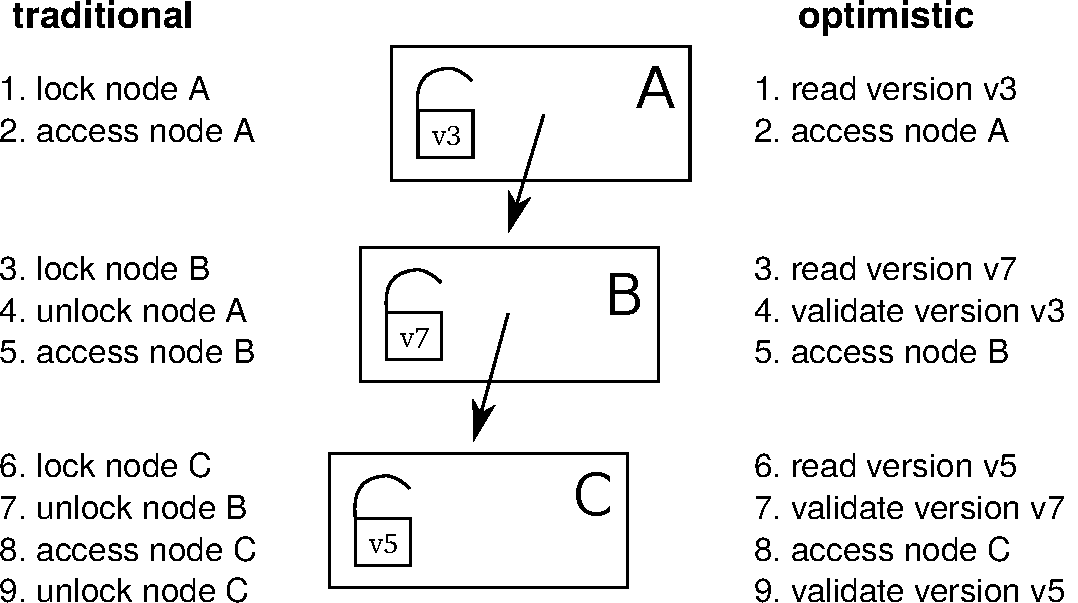
\includegraphics[width=0.65\linewidth]{olcall.pdf}
  \vspace{0.2cm}
  \caption{Comparison of a lookup operation in a 3-level tree using traditional lock coupling (left-hand side) vs.~optimistic lock coupling (right-hand side).}
  \label{fig:olc}
\end{figure}

The traditional and most common lock-based synchronization protocol for B-trees is lock coupling, which interleaves lock acquisitions while holding at most two locks at a time.
If, as we observed earlier, optimistic locks have similar semantics as traditional locks, it is natural to ask whether lock coupling can be combined with optimistic locks.
And indeed the answer is yes: One can almost mechanically translate traditional lock coupling code to optimistic lock coupling code.
This is illustrated in Figure~\ref{fig:olc}, which compares the traversal in a tree of height 3 using traditional and optimistic locks.
As the figure shows, the main difference is that locking is translated to reading the version and that unlocking becomes validation of the previously read version.
This simple change provides efficient lock-free tree traversal without the need to design a complex synchronization protocol.

It is important to emphasize the conceptual simplicity of OLC in comparison to data structures that use custom protocols like the Bw-tree~\cite{DBLP:conf/icde/LevandoskiLS13a}.
To implement lock-free access, the Bw-tree requires an indirection table, delta nodes, complex splitting and merging logic, retry logic, etc.
OLC, on the other hand, can directly be applied to B-trees mostly by adding the appropriate optimistic locking code and without modifying the node layout itself.
Therefore, OpenBw-Tree, an open source implementation of the Bw-tree, requires an order of magnitude more code than a B-tree based on OLC\footnote{Both implementations are available on GitHub: \url{https://github.com/wangziqi2016/index-microbench}}.
Given how difficult it is to develop, validate, and debug lock-free code, simplicity is obviously a major advantage.

\subsection{Correctness Aspects}

\begin{figure}
  % \centering
  %[basicstyle=\normalsize\ttfamily,showstringspaces=false,columns=fullflexible,breaklines=false,breakatwhitespace=true,numbers=none,numberstyle=\small,style=C,keepspaces=true]
\begin{lstlisting}[basicstyle=\ttfamily,language=C++,numbers=left,numberstyle=\small]
std::atomic<BTreeNode*> root;

// search for key in B+tree, returns payload in resultOut
bool lookup(Key key, Value& resultOut) {
   BTreeNode* node = root.load();
   uint64_t nodeVersion = node->readLockOrRestart();
   if (node != root.load()) // make sure the root is still the root
      restart();

   BTreeInner<Key>* parent = nullptr;
   uint64_t parentVersion = 0;

   while (node->isInner()) {
      auto inner = (BTreeInner*)node;

      // unlock parent and make current node the parent
      if (parent)
         parent->readUnlockOrRestart(parentVersion);
      parent = inner;
      parentVersion = nodeVersion;

      // search for next node
      node = inner->findChild(key);
      // validate 'inner' to ensure that 'node' pointer is valid
      inner->checkOrRestart(nodeVersion);
      // now it safe to dereference 'node' pointer (read its version)
      nodeVersion = node->readLockOrRestart();
   }

   // search in leaf and retrieve payload
   auto leaf = (BTreeLeaf*)node;
   bool success = leaf->findValue(key, resultOut);

   // unlock everything
   if (parent)
      parent->readUnlockOrRestart(parentVersion);
   node->readUnlockOrRestart(nodeVersion);

   return success;
}
\end{lstlisting}
  \vspace{0.2cm}
  \caption{B-tree lookup code using OLC. For simplicity, the restart logic is not shown.}
  \label{fig:lookup}
\end{figure}

So far, we have introduced the high-level ideas behind OLC and have stressed its similarity to traditional lock coupling.
Let us now discuss some cases where the close similarity between lock coupling and OLC breaks down.
To make this more concrete, we show the B-tree lookup code in Figure~\ref{fig:lookup}.
In the code, \texttt{readLockOrRestart} reads the lock version and \texttt{readUnlockOrRestart} validates that the read was correct.

One issue with OLC is that any pointer speculatively read from a node may point to invalid memory (if that node is modified concurrently).
Dereferencing such a pointer (e.g., to read its optimistic lock), may cause a segmentation fault or undefined behavior.
In the code shown in Figure~\ref{fig:lookup}, this problem is prevented by the extra check in line 25, which ensures that the read from the node containing the pointer was correct.
Without this additional validation, the code would in line 27 dereference the pointer speculatively read in line 23.
Note that the implementation of \texttt{checkOrRestart} is actually identical to \texttt{readUnlockOrRestart}.
We chose to give it a different name to highlight the fact that this extra check would not be necessary with read/write locks.

Another potential issue with optimistic locks is code that does not terminate.
Code that speculatively accesses a node, like an intra-node binary search, should be written in a way such that it always terminates---even in the presence of concurrent writes.
Otherwise, the validation code that detects the concurrent write will never run.
The binary search of a B-tree, for example, needs to be written in such a way that each comparison makes progress.
For some data structures that do not require loops in the traversal code (like ART) termination is trivially true.

\subsection{Implementation Details}

% implementation, efficiency
To implement an optimistic lock, one can combine the lock and the version counter into a single 64-bit\footnote{Even after subtracting one bit for the lock status, a back-of-the-envelope calculation can show that 63 bits are large enough to never overflow in practice.} word~\cite{artsync}.
A typical read operation will therefore merely consist of reading this version counter atomically.
In C++11 this can be implemented using the \texttt{std::atomic} type.

On x86, atomic reads are cheap because of x86's strong memory order guarantees.
No memory fences are required for sequentially-consistent loads, which are translated (by both GCC and clang) into standard \texttt{MOV} instructions.
Hence, the only effect of \texttt{std::atomic} for loads is preventing instruction re-ordering.
This makes version access and validation cheap.
Acquiring and releasing an optimistic lock in exclusive mode has comparable cost to a traditional lock:
A fairly expensive sequentially-consistent store is needed for acquiring a lock, while a standard \texttt{MOV} suffices for releasing it.
A simple sinlock-based implementation of optimistic locks can be found in the appendix of an earlier paper~\cite{artsync}.

OLC code must be able to handle restarts since validation or lock upgrade can fail due to concurrent writers.
Restarts can easily be implemented by wrapping the data structure operation in a loop (for simplicity not shown in Figure~\ref{fig:lookup}).
Such a loop also enables limiting the number of optimistic retry operations and falling back to pessimistic locking in cases of very heavy contention.
The ability to fall back to traditional locking is a major advantage of OLC in terms of robustness over lock-free approaches, which do not have this option.

In addition to the optimistic shared mode and the exclusive mode, optimistic locks also support a ``shared pessimistic'' mode, which physically acquires the lock in shared mode (allowing multiple concurrent readers but no writers).
This mode is useful for table (or range) scans that touch many tuples on a leaf page (which would otherwise easily abort).
Finally, let us mention that large range scans and table scans, should be broken up into several per-node traversals as is done in the LeanStore~\cite{leanstore} system.

Like all lock-free data structures, but unlike traditional locking and Hardware Transactional Memory~\cite{DBLP:conf/hpca/KarnagelDRLLSL14,DBLP:journals/pvldb/MakreshanskiLS15,htmtkde}, OLC requires care when deleting (and reusing) nodes.
The reason is that a deleting thread can never be sure that a node can be reclaimed because other threads might still be optimistically reading from that node.
Therefore, standard solutions like epoch-based reclamation~\cite{DBLP:conf/sosp/TuZKLM13}, hazard pointers~\cite{DBLP:journals/tpds/Michael04}, or optimized hazard pointers~\cite{DBLP:conf/spaa/BalmauGHZ16} need to be used.
These memory reclamation techniques are, however, largely orthogonal to the synchronization protocol itself.

%-lock-free is not a strong guarantee

\newpage
\section{Evaluation}\label{sec:evaluation}

Let us now experimentally evaluate the overhead and scalability of OLC.
For the experiments, we use an in-memory B+tree implemented in C++11 using templates, which is configured to use nodes of 4096 bytes, random 8 byte keys, and 8 byte payloads.
Based on this B-tree, we compare the following synchronization approaches:
\begin{itemize}
\item an OLC implementation\footnote{An almost identical OLC implementation is available on github: \url{https://github.com/wangziqi2016/index-microbench/tree/master/BTreeOLC}}
\item a variant based on traditional lock coupling and read/write locks
\item the unsynchronized B-tree, which obviously is only correct for read-only workloads but allows measuring the overhead of synchronization
\end{itemize}
Note that earlier work has compared the OLC implementation with a Bw-tree implementation~\cite{buzzword} and other state-of-the-art in-memory index structures.

We use a Haswell EP system with an Intel Xeon E5-2687W v3 CPU, which has 10 cores (20 ``Hyper-Threads'') and 25~MB of L3 cache.
The system is running Ubuntu 18.10 and we use GCC 8.2.0 to compile our code.
The CPU counters are obtained using the Linux perf API\footnote{We use the following convenience wrapper: \url{https://github.com/viktorleis/perfevent}}.

\begin{table}
  \caption{Performance and CPU counters for lookup and insert operations in a B-tree with 100M keys. We perform 100M operations and normalize the CPU counters by that number.}
  \label{tab:overhead}
  \centering
  \begin{tabular}{lrrrrrrr}\toprule
                    &         &        &        & instruc-  & L1     & L3     & branch \\
                    & threads & M op/s & cycles & tions & misses & misses & misses \\\midrule
lookup (no sync.)   & 1       & 1.72   & 2028   & 283     & 39.1   & 14.9   & 16.1   \\
lookup (OLC)        & 1       & 1.65   & 2107   & 370     & 43.9   & 15.1   & 16.7   \\
lookup (lock coup.) & 1       & 1.72   & 2078   & 365     & 42.3   & 16.9   & 15.7   \\\midrule
insert (no sync.)   & 1       & 1.51   & 2286   & 530     & 59.8   & 31.1   & 17.3   \\
insert (OLC)        & 1       & 1.50   & 2303   & 629     & 61.2   & 31.1   & 16.5   \\
insert (lock coup.) & 1       & 1.41   & 2473   & 644     & 61.0   & 31.0   & 17.2   \\\midrule
lookup (no sync.)   & 10      & 15.48  & 2058   & 283     & 38.6   & 15.5   & 16.0   \\
lookup (OLC)        & 10      & 14.60  & 2187   & 370     & 43.8   & 15.8   & 16.8   \\
lookup (lock coup.) & 10      & 5.71   & 5591   & 379     & 54.2   & 17.0   & 14.8   \\\midrule
insert (no sync.)   & 10      & -      & -      & -       & -      & -      & -      \\
insert (OLC)        & 10      & 10.46  & 2940   & 656     & 62.0   & 32.5   & 16.8   \\
insert (lock coup.) & 10      & 7.55   & 4161   & 667     & 75.0   & 28.6   & 16.2   \\
    \bottomrule
\end{tabular}
\end{table}

Table~\ref{tab:overhead} compares the performance and CPU counters for lookup and insert operations in a B-tree with 100M keys.
With {\em single-threaded} execution, we observe that all three approaches have very similar performance.
Adding traditional or optimistic locks to unsynchronized B-tree code results in up to 30\% of additional instructions without affecting single-threaded performance much.

\begin{figure}
  \centering
  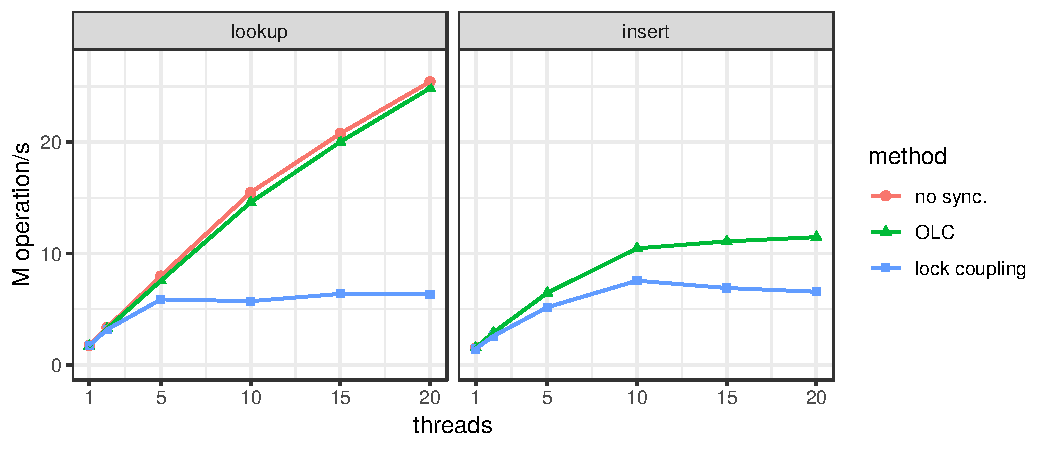
\includegraphics[width=\linewidth]{scale.pdf}
  \vspace{0.2cm}
  \caption{Scalability on 10-core system for B-tree operations (100M values).}
  \label{fig:scale}
\end{figure}

As Figure~\ref{fig:scale} shows, the results change dramatically once we use multiple threads.
For lookup, the scalability of OLC is near-linear up to 20 threads, even though the system has only 10 ``real cores''.
The OLC scalability for insert is also respectable (though not quite as linear because multi-threaded insertion approaches the memory bandwidth of our processor).
The figure also shows that the results of traditional lock coupling with read/write locks are significantly worse than OLC.
With 20 threads, lookup with OLC is 3.9$\times$ faster than traditional lock coupling.

\section{Summary}\label{sec:conc}

Optimistic Lock Coupling (OLC) is an effective synchronization method that combines the simplicity of traditional lock coupling with the superior scalability of lock-free approaches.
OLC is widely applicable and has already been successfully used to synchronize several data structures, including B-trees, binary search trees, and different trie variants.
These features make it highly attractive for modern database systems as well as performance-critical systems software in general.

\begin{thebibliography}{10}

\bibitem{DBLP:conf/spaa/BalmauGHZ16}
O.~Balmau, R.~Guerraoui, M.~Herlihy, and I.~Zablotchi.
\newblock Fast and robust memory reclamation for concurrent data structures.
\newblock In {\em SPAA}, 2016.

\bibitem{DBLP:journals/acta/BayerS77}
R.~Bayer and M.~Schkolnick.
\newblock Concurrency of operations on {B}-trees.
\newblock {\em Acta Informatica}, 9, 1977.

\bibitem{hot}
R.~Binna, E.~Zangerle, M.~Pichl, G.~Specht, and V.~Leis.
\newblock {HOT}: A height optimized trie index for main-memory database
  systems.
\newblock In {\em SIGMOD}, 2018.

\bibitem{DBLP:conf/ppopp/BronsonCCO10}
N.~G. Bronson, J.~Casper, H.~Chafi, and K.~Olukotun.
\newblock A practical concurrent binary search tree.
\newblock In {\em PPOPP}, 2010.

\bibitem{DBLP:conf/vldb/ChaHKK01}
S.~K. Cha, S.~Hwang, K.~Kim, and K.~Kwon.
\newblock Cache-conscious concurrency control of main-memory indexes on
  shared-memory multiprocessor systems.
\newblock In {\em VLDB}, 2001.

\bibitem{intel}
I.~Cutress.
\newblock {Intel} goes for 48-cores: {Cascade-AP} with multi-chip package
  coming soon.
\newblock
  \url{https://www.anandtech.com/show/13535/intel-goes-for-48cores-cascade-ap},
  2018 (accessed January, 2019).

\bibitem{DBLP:conf/cidr/FaleiroA17}
J.~M. Faleiro and D.~J. Abadi.
\newblock Latch-free synchronization in database systems: Silver bullet or
  fool's gold?
\newblock In {\em CIDR}, 2017.

\bibitem{DBLP:journals/ftdb/Graefe11}
G.~Graefe.
\newblock Modern {B}-tree techniques.
\newblock {\em Foundations and Trends in Databases}, 3(4), 2011.

\bibitem{DBLP:conf/hpca/KarnagelDRLLSL14}
T.~Karnagel, R.~Dementiev, R.~Rajwar, K.~Lai, T.~Legler, B.~Schlegel, and
  W.~Lehner.
\newblock Improving in-memory database index performance with
  {Intel}\({}^{\mbox{{\textregistered}}}\) transactional synchronization
  extensions.
\newblock In {\em HPCA}, 2014.

\bibitem{DBLP:journals/tods/LehmanY81}
P.~L. Lehman and S.~B. Yao.
\newblock Efficient locking for concurrent operations on {B}-trees.
\newblock {\em {ACM} Trans. Database Syst.}, 6(4), 1981.

\bibitem{leanstore}
V.~Leis, M.~Haubenschild, A.~Kemper, and T.~Neumann.
\newblock Leanstore: In-memory data management beyond main memory.
\newblock In {\em ICDE}, 2018.

\bibitem{art}
V.~Leis, A.~Kemper, and T.~Neumann.
\newblock The adaptive radix tree: {ARTful} indexing for main-memory databases.
\newblock In {\em ICDE}, 2013.

\bibitem{htmtkde}
V.~Leis, A.~Kemper, and T.~Neumann.
\newblock Scaling {HTM}-supported database transactions to many cores.
\newblock {\em {IEEE} Trans. Knowl. Data Eng.}, 28(2), 2016.

\bibitem{artsync}
V.~Leis, F.~Scheibner, A.~Kemper, and T.~Neumann.
\newblock The {ART} of practical synchronization.
\newblock In {\em DaMoN}, 2016.

\bibitem{DBLP:conf/icde/LevandoskiLS13a}
J.~J. Levandoski, D.~B. Lomet, and S.~Sengupta.
\newblock The {Bw}-tree: A {B}-tree for new hardware platforms.
\newblock In {\em ICDE}, 2013.

\bibitem{DBLP:journals/pvldb/MakreshanskiLS15}
D.~Makreshanski, J.~J. Levandoski, and R.~Stutsman.
\newblock To lock, swap, or elide: On the interplay of hardware transactional
  memory and lock-free indexing.
\newblock {\em {PVLDB}}, 8(11), 2015.

\bibitem{DBLP:dblp_conf/eurosys/MaoKM12}
Y.~Mao, E.~Kohler, and R.~T. Morris.
\newblock Cache craftiness for fast multicore key-value storage.
\newblock In {\em EuroSys}, 2012.

\bibitem{DBLP:journals/tpds/Michael04}
M.~M. Michael.
\newblock Hazard pointers: Safe memory reclamation for lock-free objects.
\newblock {\em {IEEE} Trans. Parallel Distrib. Syst.}, 15(6), 2004.

\bibitem{DBLP:journals/jacm/ShalevS06}
O.~Shalev and N.~Shavit.
\newblock Split-ordered lists: Lock-free extensible hash tables.
\newblock {\em J. {ACM}}, 53(3), 2006.

\bibitem{amd}
A.~Shilov.
\newblock {AMD} previews {EPYC} ‘{Rome}’ processor: Up to 64 {Zen} 2 cores.
\newblock
  \url{https://www.anandtech.com/show/13561/amd-previews-epyc-rome-processor-up-to-64-zen-2-cores},
  2018 (accessed January, 2019).

\bibitem{DBLP:conf/sosp/TuZKLM13}
S.~Tu, W.~Zheng, E.~Kohler, B.~Liskov, and S.~Madden.
\newblock Speedy transactions in multicore in-memory databases.
\newblock In {\em SOSP}, 2013.

\bibitem{buzzword}
Z.~Wang, A.~Pavlo, H.~Lim, V.~Leis, H.~Zhang, M.~Kaminsky, and D.~Andersen.
\newblock Building a {Bw}-tree takes more than just buzz words.
\newblock In {\em SIGMOD}, 2018.

\end{thebibliography}


%\bibliographystyle{abbrv}
%\bibliography{main}

\end{document}

\end{article}

\begin{article}
{User Interfaces for Exploratory Data Analysis: A Survey of Open-Source and Commercial Tools}
{Jinglin Peng, Weiyuan Wu, Jing Nathan Yan, Danrui Qi, Jeffrey M.\ Rzeszotarski, and Jiannan Wang}
\pdfminorversion=5
\documentclass[11pt]{article}
\usepackage{deauthor,times,graphicx,caption,microtype}
\usepackage{hyperref}
\usepackage{listings}
\usepackage{booktabs}

\begin{document}

\title{Optimistic Lock Coupling: A Scalable and Efficient General-Purpose Synchronization Method}

\author{Viktor Leis, Michael Haubenschild\raisebox{0.9ex}{$\ast$}, Thomas Neumann\\ Technische Universit{\"a}t M{\"u}nchen \hspace{0.7cm} Tableau Software\raisebox{0.9ex}{$\ast$} \\ {\{leis,neumann\}{@}in.tum.de} \hspace{0.7cm} {mhaubenschild{@}tableau.com\raisebox{0.9ex}{$\ast$}}}

\maketitle

\begin{abstract}
As the number of cores on commodity processors continues to increase, scalability becomes more and more crucial for overall performance.
Scalable and efficient concurrent data structures are particularly important, as these are often the building blocks of parallel algorithms.
Unfortunately, traditional synchronization techniques based on fine-grained locking have been shown to be unscalable on modern multi-core CPUs.
Lock-free data structures, on the other hand, are extremely difficult to design and often incur significant overhead.

In this work, we make the case for Optimistic Lock Coupling as a practical alternative to both traditional locking and the lock-free approach.
We show that Optimistic Lock Coupling is highly scalable and almost as simple to implement as traditional lock coupling.
Another important advantage is that it is easily applicable to most tree-like data structures.
We therefore argue that Optimistic Lock Coupling, rather than a complex and error-prone custom synchronization protocol, should be the default choice for performance-critical data structures.
\end{abstract}

\section{Introduction}

% more and more cores
Today, Intel's commodity server processors have up to 28 cores and its upcoming microarchitecture will have up to 48 cores per socket~\cite{intel}.
Similarly, AMD currently stands at 32 cores and this number is expected to double in the next generation~\cite{amd}.
Since both platforms support simultaneous multithreading (also known as hyperthreading), affordable commodity servers (with up to two sockets) will soon routinely have between 100 and 200 hardware threads.

% data structure scalability is important
With such a high degree of hardware parallelism, efficient data processing crucially depends on how well concurrent data structures scale.
Internally, database systems use a plethora of data structures like table heaps, internal work queues, and, most importantly, index structures.
Any of these can easily become a scalability (and therefore overall performance) bottleneck on many-core CPUs.

% traditional synchronization: fine-grained locks, slow, cache invalidation
Traditionally, database systems synchronize internal data structures using fine-grained reader/writer locks\footnote{In this work, we focus on data structure synchronization rather than high-level transaction semantics and therefore use the term {\em lock} for what would typically be called {\em latch} in the database literature. We thus follow common computer science (rather than database) terminology.}.
Unfortunately, while fine-grained locking makes lock contention unlikely, it still results in bad scalability because lock acquisition and release require writing to shared memory.
Due to the way cache coherency is implemented on modern multi-core CPUs, these writes cause additional cache misses\footnote{The cache coherency protocol ensures that all copies of a cache line on other cores are invalidated before the write can proceed.} and the cache line containing the lock's internal data becomes a point of physical contention.
As a result, any frequently-accessed lock (e.g., the lock of the root node of a B-tree) severely limits scalability.

% lock-free bw-tree: no more latches, but indirections, extremely complex
Lock-free data structures like the Bw-tree~\cite{DBLP:conf/icde/LevandoskiLS13a} (a lock-free B-tree variant) or the Split-Ordered List~\cite{DBLP:journals/jacm/ShalevS06} (a lock-free hash table) do not acquire any locks and therefore generally scale much better than locking-based approaches (in particular for read-mostly workloads).
However, lock-free synchronization has other downsides:
First, it is very difficult and results in extremely complex and error-prone code (when compared to locking).
Second, because the functionality of atomic primitives provided by the hardware (e.g., atomically compare-and-swap 8 bytes) is limited, complex operations require additional indirections within the data structure.
For example, the Bw-tree requires an indirection table and the Split-Ordered List requires ``dummy nodes'', resulting in overhead due to additional cache misses.

% OLC for the win
In this paper we make the case for {\em Optimistic Lock Coupling (OLC)}, a synchronization method that combines some of the best properties of lock-based and lock-free synchronization.
OLC utilizes a special lock type that can be used in two modes:
The first mode is similar to a traditional mutex and excludes other threads by physically acquiring the underlying lock.
In the second mode, reads can proceed optimistically by validating a version counter that is embedded in the lock (similar to optimistic concurrency control).
The first mode is typically used by writers and the second mode by readers.
Besides this special lock type, OLC is based on the observation that optimistic lock validations can be interleaved/coupled---similar to the pair-wise interleaved lock acquisition of traditional lock coupling.
Hence, the name Optimistic Lock Coupling.

OLC has a number of desirable features:
\begin{itemize}
\item By reducing the number of writes to shared memory locations and thereby avoiding cache invalidations, it {\bf scales well} for most workloads.
\item In comparison to unsynchronized code, it requires few additional CPU instructions making it {\bf efficient}.
\item OLC is {\bf widely applicable} to different data structures. It has already been successfully used for synchronizing binary search trees~\cite{DBLP:conf/ppopp/BronsonCCO10}, tries~\cite{artsync}, trie/B-tree hybrids~\cite{DBLP:dblp_conf/eurosys/MaoKM12}, and B-trees~\cite{buzzword}.
\item In comparison to the lock-free paradigm, it is also {\bf easy to use} and requires few modifications to existing, single-threaded data structures.
\end{itemize}
Despite these positive features and its simplicity, OLC is not yet widely known.
The goal of this paper is therefore to popularize this simple idea and to make a case for it.
We argue that OLC deserves to be widely known.
It is a good default synchronization paradigm---more complex, data structure-specific protocols are seldom beneficial.

The rest of the paper is organized as follows.
Section~\ref{sec:related} discusses related work, tracing the history of OLC and its underlying ideas in the literature.
The core of the paper is Section~\ref{sec:olc}, which describes the ideas behind OLC and how it can be used to synchronize complex data structures.
In Section~\ref{sec:evaluation} we experimentally show that OLC has low overhead and scales well when used to synchronize an in-memory B-tree.
We summarize the paper in Section~\ref{sec:conc}.

\newpage
\section{Related Work}\label{sec:related}

Lock coupling has been proposed as a method for allowing concurrent operations on B-trees in 1977~\cite{DBLP:journals/acta/BayerS77}.
This traditional and still widely-used method, described in detail in Graefe's B-tree survey~\cite{DBLP:journals/ftdb/Graefe11}, is also called ``latch coupling'', ``hand-over-hand locking'', and ``crabbing''.
Because at most two locks are held at-a-time during tree traversal, this technique seemingly allows for a high degree of parallelism---in particular if read/write locks are used to enable inner nodes to be locked in shared mode.
However, as we show in Section~\ref{sec:evaluation}, on modern hardware lock acquisition (even in shared mode) results in suboptimal scalability.

An early alternative from 1981 is a B-tree variant called B-link tree~\cite{DBLP:journals/tods/LehmanY81}, which only holds a single lock at a time.
It is based on the observation that between the release of the parent lock and the acquisition of the child lock, the only ``dangerous'' thing that could have happened is the split of a child node (assuming one does not implement merge operations).
Thus, when a split happens, the key being searched might end up on a neighboring node to the right of the current child node.
A B-link tree traversal therefore detects this condition and, if needed, transparently proceeds to the neighboring node.
Releasing the parent lock early is highly beneficial when the child node needs to be fetched from disk.
For in-memory workloads, however, the B-link tree has the same scalability issues as lock coupling (it acquires just as many locks).

The next major advance, Optimistic Latch-Free Index Traversal (OLFIT)~\cite{DBLP:conf/vldb/ChaHKK01}, was proposed in 2001.
OLFIT introduced the idea of a combined lock/update counter, which we call {\em optimistic lock}. % , for lack of a better name,
Based on these per-node optimistic locks and the synchronization protocol of the B-link tree, OLFIT finally achieves good scalability on parallel processors.
The OLFIT protocol is fairly complex, as it requires both the non-trivial B-link protocol and optimistic locks.
Furthermore, like the B-link tree protocol, it does not support merging nodes, and is specific to B-trees (cannot easily be applied to other data structures).

In the following two decades, the growth of main-memory capacity led to much research into other data structures besides the venerable B-tree.
Particularly relevant for our discussion is Bronson et al.'s~\cite{DBLP:conf/ppopp/BronsonCCO10} concurrent binary search tree, which is based on optimistic version validation and has a sophisticated, data structure-specific synchronization protocol.
To the best of our knowledge, this 2010 paper is the first that, as part of its protocol, interleaves version validation across nodes---rather than validating each node separately like OLFIT.
In that paper, this idea is called ``hand-over-hand, optimistic validation'', while we prefer the term Optimistic Lock Coupling to highlight the close resemblance to traditional lock coupling.
Similarly, Mao et al.'s~\cite{DBLP:dblp_conf/eurosys/MaoKM12} Masstree (a concurrent hybrid trie/B-tree) is also based on the same ideas, but again uses them as part of a more complex protocol.

The Adaptive Radix Tree (ART)~\cite{art} is another recent in-memory data structure, which we proposed in 2013.
In contrast to the two data structures just mentioned, it was originally designed with single-threaded performance in mind without supporting concurrency.
To add support for concurrency, we initially started designing a custom protocol called Read-Optimized Write Exclusion (ROWEX)~\cite{artsync}, which turned out to be non-trivial and requires modifications of the underlying data structure\footnote{Note that ROWEX is already easier to apply to existing data structures than the lock-free approach. The difficulty depends on the data structure. Applying ROWEX is hard for B-trees with sorted keys and fairly easy for copy-on-write data structures like the Height Optimized Trie~\cite{hot}---with ART being somewhere in the middle.}.
However, fairly late in the project, we also realized, that OLC {\em alone} (rather than as part of a more complex protocol) is sufficient to synchronize ART.
No other changes to the data structure were necessary.
Both approaches were published and experimentally evaluated in a followup paper~\cite{artsync}, which shows that, despite its simplicity, OLC is efficient, scalable, and generally outperforms ROWEX.

Similar results were recently published regarding B-trees~\cite{buzzword}.
In this experimental study a simple OLC-based synchronization outperformed the Bw-tree~\cite{DBLP:conf/icde/LevandoskiLS13a}, a complex lock-free synchronization approach.
Another recent paper shows that for write-intensive workloads, locking often performs better than lock-free synchronization~\cite{DBLP:conf/cidr/FaleiroA17}.
These experiences indicate that OLC is a general-purpose synchronization paradigm and motivate the current paper.

%foster b-tree\cite{DBLP:journals/tods/GraefeKK12}
%Shasha theory~\cite{DBLP:journals/tods/ShashaG88}

\section{Optimistic Lock Coupling}\label{sec:olc}

% locks suck
The standard technique for inter-thread synchronization is mutual exclusion using fine-grained locks.
In a B-tree, for example, every node usually has its own associated lock, which is acquired before accessing that node.
The problem of locking on modern multi- and many-core processors is that lock acquisition and release require writing to the shared memory location that implements the lock.
This write causes exclusive ownership of the underlying cache line and invalidates copies of it on all other processor cores.
For hierarchical, tree-like data structures, the lock of the root node becomes a point of physical contention---even in read-only workloads and even when read/write locks are used.
Depending on the specific data structure, number of cores, cache coherency protocol implementation, cache topology, whether Non-Uniform Memory Access (NUMA) is used, locking can even result in multi-threaded performance that is worse than single-threaded execution.

% in b-trees this happens very much
The inherent pessimism of locking is particularly unfortunate for B-trees:
Despite the fact that logical modifications of the root node are very infrequent, every B-tree operation must lock the root node during tree traversal\footnote{To a lesser extent this obviously applies to all inner nodes, not just the root.}.
Even the vast majority of update operations (with the exception of splits and merges), only modify a single leaf node.
These observations indicate that a more optimistic approach, which does not require locking inner nodes, would be very beneficial for B-trees.

\subsection{Optimistic Locks}

% optimism to the rescue
As the name indicates, optimistic locks try to solve the scalability issues of traditional locks using an optimistic approach.
Instead of always physically acquiring locks, even for nodes that are unlikely to be modified simultaneously, after-the-fact validation is used to detect conflicts.
This is done by augmenting each lock with a version/update counter that is incremented on every modification.
Using this version counter, readers can optimistically proceed before validating that the version did not change to ensure that the read was safe.
If validation fails, the operation is restarted.

% details on opt locks
Using optimistic locks, a read-only node access (i.e., the majority of all operations in a B-tree) does not acquire the lock and does not increment the version counter.
Instead, it performs the following steps:
\begin{enumerate}
\item read lock version (restart if lock is not free)
\item access node
\item read the version again and validate that it has not changed in the meantime
\end{enumerate}
If the last step (the validation) fails, the operation has to be restarted.
Write operations, on the other hand, are more similar to traditional locking:
\begin{enumerate}
\item acquire lock (wait if necessary)
\item access/write to node
\item increment version and unlock node
\end{enumerate}
Writes can therefore protect a node from other writes.

% similar to locks
As we observed in an earlier paper~\cite{artsync}, because of similar semantics, optimistic locks can be hidden behind an API very similar to traditional read/write locks.
Both approaches have an exclusive lock mode, and acquiring a traditional lock in shared mode is analogous to optimistic version validation.
Furthermore, like with some implementations of traditional read/write locks, optimistic locks allow upgrading a shared lock to an exclusive lock.
Lock upgrades are, for example, used to avoid most B-tree update operations from having to lock inner nodes.
In our experience, the close resemblance of optimistic and traditional locks simplifies the reasoning about optimistic locks;
one can apply similar thinking as in traditional lock-based protocols.

\subsection{Lock Coupling with Optimistic Locks}

\begin{figure}
  \centering
  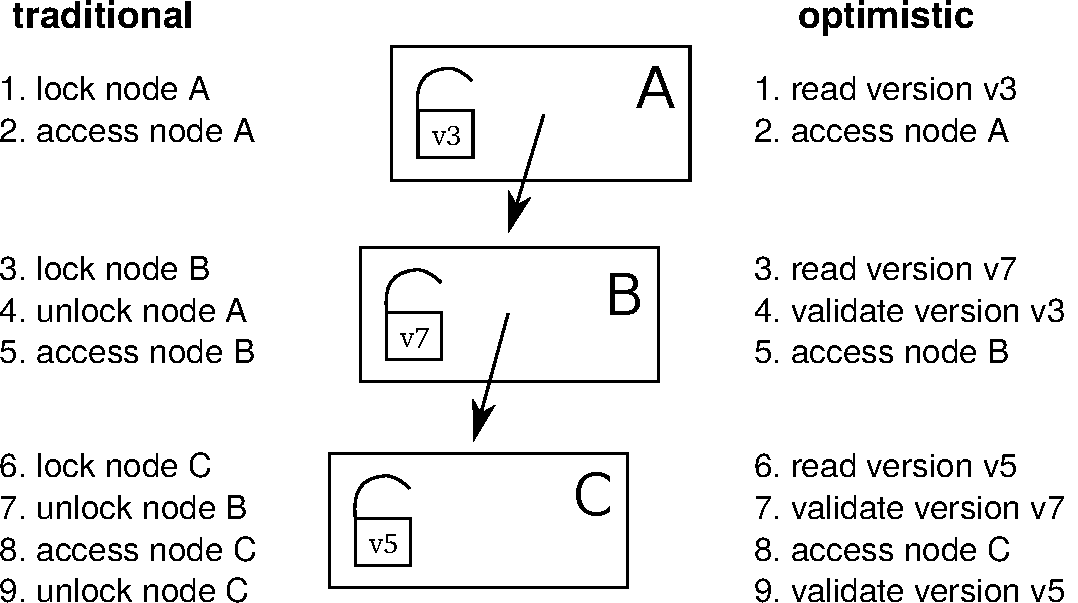
\includegraphics[width=0.65\linewidth]{olcall.pdf}
  \vspace{0.2cm}
  \caption{Comparison of a lookup operation in a 3-level tree using traditional lock coupling (left-hand side) vs.~optimistic lock coupling (right-hand side).}
  \label{fig:olc}
\end{figure}

The traditional and most common lock-based synchronization protocol for B-trees is lock coupling, which interleaves lock acquisitions while holding at most two locks at a time.
If, as we observed earlier, optimistic locks have similar semantics as traditional locks, it is natural to ask whether lock coupling can be combined with optimistic locks.
And indeed the answer is yes: One can almost mechanically translate traditional lock coupling code to optimistic lock coupling code.
This is illustrated in Figure~\ref{fig:olc}, which compares the traversal in a tree of height 3 using traditional and optimistic locks.
As the figure shows, the main difference is that locking is translated to reading the version and that unlocking becomes validation of the previously read version.
This simple change provides efficient lock-free tree traversal without the need to design a complex synchronization protocol.

It is important to emphasize the conceptual simplicity of OLC in comparison to data structures that use custom protocols like the Bw-tree~\cite{DBLP:conf/icde/LevandoskiLS13a}.
To implement lock-free access, the Bw-tree requires an indirection table, delta nodes, complex splitting and merging logic, retry logic, etc.
OLC, on the other hand, can directly be applied to B-trees mostly by adding the appropriate optimistic locking code and without modifying the node layout itself.
Therefore, OpenBw-Tree, an open source implementation of the Bw-tree, requires an order of magnitude more code than a B-tree based on OLC\footnote{Both implementations are available on GitHub: \url{https://github.com/wangziqi2016/index-microbench}}.
Given how difficult it is to develop, validate, and debug lock-free code, simplicity is obviously a major advantage.

\subsection{Correctness Aspects}

\begin{figure}
  % \centering
  %[basicstyle=\normalsize\ttfamily,showstringspaces=false,columns=fullflexible,breaklines=false,breakatwhitespace=true,numbers=none,numberstyle=\small,style=C,keepspaces=true]
\begin{lstlisting}[basicstyle=\ttfamily,language=C++,numbers=left,numberstyle=\small]
std::atomic<BTreeNode*> root;

// search for key in B+tree, returns payload in resultOut
bool lookup(Key key, Value& resultOut) {
   BTreeNode* node = root.load();
   uint64_t nodeVersion = node->readLockOrRestart();
   if (node != root.load()) // make sure the root is still the root
      restart();

   BTreeInner<Key>* parent = nullptr;
   uint64_t parentVersion = 0;

   while (node->isInner()) {
      auto inner = (BTreeInner*)node;

      // unlock parent and make current node the parent
      if (parent)
         parent->readUnlockOrRestart(parentVersion);
      parent = inner;
      parentVersion = nodeVersion;

      // search for next node
      node = inner->findChild(key);
      // validate 'inner' to ensure that 'node' pointer is valid
      inner->checkOrRestart(nodeVersion);
      // now it safe to dereference 'node' pointer (read its version)
      nodeVersion = node->readLockOrRestart();
   }

   // search in leaf and retrieve payload
   auto leaf = (BTreeLeaf*)node;
   bool success = leaf->findValue(key, resultOut);

   // unlock everything
   if (parent)
      parent->readUnlockOrRestart(parentVersion);
   node->readUnlockOrRestart(nodeVersion);

   return success;
}
\end{lstlisting}
  \vspace{0.2cm}
  \caption{B-tree lookup code using OLC. For simplicity, the restart logic is not shown.}
  \label{fig:lookup}
\end{figure}

So far, we have introduced the high-level ideas behind OLC and have stressed its similarity to traditional lock coupling.
Let us now discuss some cases where the close similarity between lock coupling and OLC breaks down.
To make this more concrete, we show the B-tree lookup code in Figure~\ref{fig:lookup}.
In the code, \texttt{readLockOrRestart} reads the lock version and \texttt{readUnlockOrRestart} validates that the read was correct.

One issue with OLC is that any pointer speculatively read from a node may point to invalid memory (if that node is modified concurrently).
Dereferencing such a pointer (e.g., to read its optimistic lock), may cause a segmentation fault or undefined behavior.
In the code shown in Figure~\ref{fig:lookup}, this problem is prevented by the extra check in line 25, which ensures that the read from the node containing the pointer was correct.
Without this additional validation, the code would in line 27 dereference the pointer speculatively read in line 23.
Note that the implementation of \texttt{checkOrRestart} is actually identical to \texttt{readUnlockOrRestart}.
We chose to give it a different name to highlight the fact that this extra check would not be necessary with read/write locks.

Another potential issue with optimistic locks is code that does not terminate.
Code that speculatively accesses a node, like an intra-node binary search, should be written in a way such that it always terminates---even in the presence of concurrent writes.
Otherwise, the validation code that detects the concurrent write will never run.
The binary search of a B-tree, for example, needs to be written in such a way that each comparison makes progress.
For some data structures that do not require loops in the traversal code (like ART) termination is trivially true.

\subsection{Implementation Details}

% implementation, efficiency
To implement an optimistic lock, one can combine the lock and the version counter into a single 64-bit\footnote{Even after subtracting one bit for the lock status, a back-of-the-envelope calculation can show that 63 bits are large enough to never overflow in practice.} word~\cite{artsync}.
A typical read operation will therefore merely consist of reading this version counter atomically.
In C++11 this can be implemented using the \texttt{std::atomic} type.

On x86, atomic reads are cheap because of x86's strong memory order guarantees.
No memory fences are required for sequentially-consistent loads, which are translated (by both GCC and clang) into standard \texttt{MOV} instructions.
Hence, the only effect of \texttt{std::atomic} for loads is preventing instruction re-ordering.
This makes version access and validation cheap.
Acquiring and releasing an optimistic lock in exclusive mode has comparable cost to a traditional lock:
A fairly expensive sequentially-consistent store is needed for acquiring a lock, while a standard \texttt{MOV} suffices for releasing it.
A simple sinlock-based implementation of optimistic locks can be found in the appendix of an earlier paper~\cite{artsync}.

OLC code must be able to handle restarts since validation or lock upgrade can fail due to concurrent writers.
Restarts can easily be implemented by wrapping the data structure operation in a loop (for simplicity not shown in Figure~\ref{fig:lookup}).
Such a loop also enables limiting the number of optimistic retry operations and falling back to pessimistic locking in cases of very heavy contention.
The ability to fall back to traditional locking is a major advantage of OLC in terms of robustness over lock-free approaches, which do not have this option.

In addition to the optimistic shared mode and the exclusive mode, optimistic locks also support a ``shared pessimistic'' mode, which physically acquires the lock in shared mode (allowing multiple concurrent readers but no writers).
This mode is useful for table (or range) scans that touch many tuples on a leaf page (which would otherwise easily abort).
Finally, let us mention that large range scans and table scans, should be broken up into several per-node traversals as is done in the LeanStore~\cite{leanstore} system.

Like all lock-free data structures, but unlike traditional locking and Hardware Transactional Memory~\cite{DBLP:conf/hpca/KarnagelDRLLSL14,DBLP:journals/pvldb/MakreshanskiLS15,htmtkde}, OLC requires care when deleting (and reusing) nodes.
The reason is that a deleting thread can never be sure that a node can be reclaimed because other threads might still be optimistically reading from that node.
Therefore, standard solutions like epoch-based reclamation~\cite{DBLP:conf/sosp/TuZKLM13}, hazard pointers~\cite{DBLP:journals/tpds/Michael04}, or optimized hazard pointers~\cite{DBLP:conf/spaa/BalmauGHZ16} need to be used.
These memory reclamation techniques are, however, largely orthogonal to the synchronization protocol itself.

%-lock-free is not a strong guarantee

\newpage
\section{Evaluation}\label{sec:evaluation}

Let us now experimentally evaluate the overhead and scalability of OLC.
For the experiments, we use an in-memory B+tree implemented in C++11 using templates, which is configured to use nodes of 4096 bytes, random 8 byte keys, and 8 byte payloads.
Based on this B-tree, we compare the following synchronization approaches:
\begin{itemize}
\item an OLC implementation\footnote{An almost identical OLC implementation is available on github: \url{https://github.com/wangziqi2016/index-microbench/tree/master/BTreeOLC}}
\item a variant based on traditional lock coupling and read/write locks
\item the unsynchronized B-tree, which obviously is only correct for read-only workloads but allows measuring the overhead of synchronization
\end{itemize}
Note that earlier work has compared the OLC implementation with a Bw-tree implementation~\cite{buzzword} and other state-of-the-art in-memory index structures.

We use a Haswell EP system with an Intel Xeon E5-2687W v3 CPU, which has 10 cores (20 ``Hyper-Threads'') and 25~MB of L3 cache.
The system is running Ubuntu 18.10 and we use GCC 8.2.0 to compile our code.
The CPU counters are obtained using the Linux perf API\footnote{We use the following convenience wrapper: \url{https://github.com/viktorleis/perfevent}}.

\begin{table}
  \caption{Performance and CPU counters for lookup and insert operations in a B-tree with 100M keys. We perform 100M operations and normalize the CPU counters by that number.}
  \label{tab:overhead}
  \centering
  \begin{tabular}{lrrrrrrr}\toprule
                    &         &        &        & instruc-  & L1     & L3     & branch \\
                    & threads & M op/s & cycles & tions & misses & misses & misses \\\midrule
lookup (no sync.)   & 1       & 1.72   & 2028   & 283     & 39.1   & 14.9   & 16.1   \\
lookup (OLC)        & 1       & 1.65   & 2107   & 370     & 43.9   & 15.1   & 16.7   \\
lookup (lock coup.) & 1       & 1.72   & 2078   & 365     & 42.3   & 16.9   & 15.7   \\\midrule
insert (no sync.)   & 1       & 1.51   & 2286   & 530     & 59.8   & 31.1   & 17.3   \\
insert (OLC)        & 1       & 1.50   & 2303   & 629     & 61.2   & 31.1   & 16.5   \\
insert (lock coup.) & 1       & 1.41   & 2473   & 644     & 61.0   & 31.0   & 17.2   \\\midrule
lookup (no sync.)   & 10      & 15.48  & 2058   & 283     & 38.6   & 15.5   & 16.0   \\
lookup (OLC)        & 10      & 14.60  & 2187   & 370     & 43.8   & 15.8   & 16.8   \\
lookup (lock coup.) & 10      & 5.71   & 5591   & 379     & 54.2   & 17.0   & 14.8   \\\midrule
insert (no sync.)   & 10      & -      & -      & -       & -      & -      & -      \\
insert (OLC)        & 10      & 10.46  & 2940   & 656     & 62.0   & 32.5   & 16.8   \\
insert (lock coup.) & 10      & 7.55   & 4161   & 667     & 75.0   & 28.6   & 16.2   \\
    \bottomrule
\end{tabular}
\end{table}

Table~\ref{tab:overhead} compares the performance and CPU counters for lookup and insert operations in a B-tree with 100M keys.
With {\em single-threaded} execution, we observe that all three approaches have very similar performance.
Adding traditional or optimistic locks to unsynchronized B-tree code results in up to 30\% of additional instructions without affecting single-threaded performance much.

\begin{figure}
  \centering
  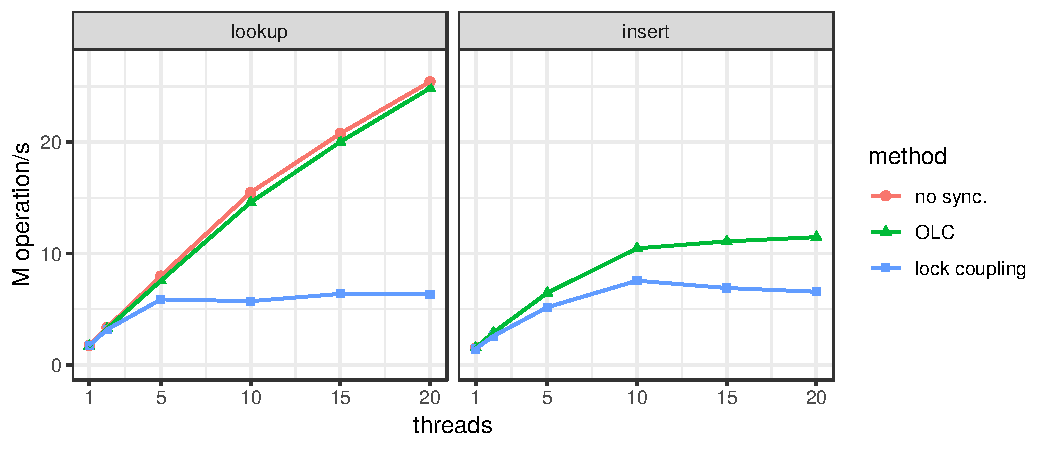
\includegraphics[width=\linewidth]{scale.pdf}
  \vspace{0.2cm}
  \caption{Scalability on 10-core system for B-tree operations (100M values).}
  \label{fig:scale}
\end{figure}

As Figure~\ref{fig:scale} shows, the results change dramatically once we use multiple threads.
For lookup, the scalability of OLC is near-linear up to 20 threads, even though the system has only 10 ``real cores''.
The OLC scalability for insert is also respectable (though not quite as linear because multi-threaded insertion approaches the memory bandwidth of our processor).
The figure also shows that the results of traditional lock coupling with read/write locks are significantly worse than OLC.
With 20 threads, lookup with OLC is 3.9$\times$ faster than traditional lock coupling.

\section{Summary}\label{sec:conc}

Optimistic Lock Coupling (OLC) is an effective synchronization method that combines the simplicity of traditional lock coupling with the superior scalability of lock-free approaches.
OLC is widely applicable and has already been successfully used to synchronize several data structures, including B-trees, binary search trees, and different trie variants.
These features make it highly attractive for modern database systems as well as performance-critical systems software in general.

\begin{thebibliography}{10}

\bibitem{DBLP:conf/spaa/BalmauGHZ16}
O.~Balmau, R.~Guerraoui, M.~Herlihy, and I.~Zablotchi.
\newblock Fast and robust memory reclamation for concurrent data structures.
\newblock In {\em SPAA}, 2016.

\bibitem{DBLP:journals/acta/BayerS77}
R.~Bayer and M.~Schkolnick.
\newblock Concurrency of operations on {B}-trees.
\newblock {\em Acta Informatica}, 9, 1977.

\bibitem{hot}
R.~Binna, E.~Zangerle, M.~Pichl, G.~Specht, and V.~Leis.
\newblock {HOT}: A height optimized trie index for main-memory database
  systems.
\newblock In {\em SIGMOD}, 2018.

\bibitem{DBLP:conf/ppopp/BronsonCCO10}
N.~G. Bronson, J.~Casper, H.~Chafi, and K.~Olukotun.
\newblock A practical concurrent binary search tree.
\newblock In {\em PPOPP}, 2010.

\bibitem{DBLP:conf/vldb/ChaHKK01}
S.~K. Cha, S.~Hwang, K.~Kim, and K.~Kwon.
\newblock Cache-conscious concurrency control of main-memory indexes on
  shared-memory multiprocessor systems.
\newblock In {\em VLDB}, 2001.

\bibitem{intel}
I.~Cutress.
\newblock {Intel} goes for 48-cores: {Cascade-AP} with multi-chip package
  coming soon.
\newblock
  \url{https://www.anandtech.com/show/13535/intel-goes-for-48cores-cascade-ap},
  2018 (accessed January, 2019).

\bibitem{DBLP:conf/cidr/FaleiroA17}
J.~M. Faleiro and D.~J. Abadi.
\newblock Latch-free synchronization in database systems: Silver bullet or
  fool's gold?
\newblock In {\em CIDR}, 2017.

\bibitem{DBLP:journals/ftdb/Graefe11}
G.~Graefe.
\newblock Modern {B}-tree techniques.
\newblock {\em Foundations and Trends in Databases}, 3(4), 2011.

\bibitem{DBLP:conf/hpca/KarnagelDRLLSL14}
T.~Karnagel, R.~Dementiev, R.~Rajwar, K.~Lai, T.~Legler, B.~Schlegel, and
  W.~Lehner.
\newblock Improving in-memory database index performance with
  {Intel}\({}^{\mbox{{\textregistered}}}\) transactional synchronization
  extensions.
\newblock In {\em HPCA}, 2014.

\bibitem{DBLP:journals/tods/LehmanY81}
P.~L. Lehman and S.~B. Yao.
\newblock Efficient locking for concurrent operations on {B}-trees.
\newblock {\em {ACM} Trans. Database Syst.}, 6(4), 1981.

\bibitem{leanstore}
V.~Leis, M.~Haubenschild, A.~Kemper, and T.~Neumann.
\newblock Leanstore: In-memory data management beyond main memory.
\newblock In {\em ICDE}, 2018.

\bibitem{art}
V.~Leis, A.~Kemper, and T.~Neumann.
\newblock The adaptive radix tree: {ARTful} indexing for main-memory databases.
\newblock In {\em ICDE}, 2013.

\bibitem{htmtkde}
V.~Leis, A.~Kemper, and T.~Neumann.
\newblock Scaling {HTM}-supported database transactions to many cores.
\newblock {\em {IEEE} Trans. Knowl. Data Eng.}, 28(2), 2016.

\bibitem{artsync}
V.~Leis, F.~Scheibner, A.~Kemper, and T.~Neumann.
\newblock The {ART} of practical synchronization.
\newblock In {\em DaMoN}, 2016.

\bibitem{DBLP:conf/icde/LevandoskiLS13a}
J.~J. Levandoski, D.~B. Lomet, and S.~Sengupta.
\newblock The {Bw}-tree: A {B}-tree for new hardware platforms.
\newblock In {\em ICDE}, 2013.

\bibitem{DBLP:journals/pvldb/MakreshanskiLS15}
D.~Makreshanski, J.~J. Levandoski, and R.~Stutsman.
\newblock To lock, swap, or elide: On the interplay of hardware transactional
  memory and lock-free indexing.
\newblock {\em {PVLDB}}, 8(11), 2015.

\bibitem{DBLP:dblp_conf/eurosys/MaoKM12}
Y.~Mao, E.~Kohler, and R.~T. Morris.
\newblock Cache craftiness for fast multicore key-value storage.
\newblock In {\em EuroSys}, 2012.

\bibitem{DBLP:journals/tpds/Michael04}
M.~M. Michael.
\newblock Hazard pointers: Safe memory reclamation for lock-free objects.
\newblock {\em {IEEE} Trans. Parallel Distrib. Syst.}, 15(6), 2004.

\bibitem{DBLP:journals/jacm/ShalevS06}
O.~Shalev and N.~Shavit.
\newblock Split-ordered lists: Lock-free extensible hash tables.
\newblock {\em J. {ACM}}, 53(3), 2006.

\bibitem{amd}
A.~Shilov.
\newblock {AMD} previews {EPYC} ‘{Rome}’ processor: Up to 64 {Zen} 2 cores.
\newblock
  \url{https://www.anandtech.com/show/13561/amd-previews-epyc-rome-processor-up-to-64-zen-2-cores},
  2018 (accessed January, 2019).

\bibitem{DBLP:conf/sosp/TuZKLM13}
S.~Tu, W.~Zheng, E.~Kohler, B.~Liskov, and S.~Madden.
\newblock Speedy transactions in multicore in-memory databases.
\newblock In {\em SOSP}, 2013.

\bibitem{buzzword}
Z.~Wang, A.~Pavlo, H.~Lim, V.~Leis, H.~Zhang, M.~Kaminsky, and D.~Andersen.
\newblock Building a {Bw}-tree takes more than just buzz words.
\newblock In {\em SIGMOD}, 2018.

\end{thebibliography}


%\bibliographystyle{abbrv}
%\bibliography{main}

\end{document}

\end{article}

\begin{article}
{The Right Tool for the Job: Data-Centric Workflows in Vizier}
{Oliver Kennedy, Boris Glavic, Juliana Freire, and Michael Brachmann}
\documentclass[11pt]{article}

\usepackage{deauthor,times,graphicx}
\usepackage{color,colortbl}
% \usepackage[dvipsnames]{xcolor}
% \usepackage{hyperref}
\usepackage{amsmath}
\usepackage{amssymb}
\let\proof\relax
\let\endproof\relax
\usepackage{amsthm}
\usepackage{cleveref}
\usepackage{wrapfig}
\usepackage{url}
\usepackage{stmaryrd,amssymb}
\usepackage{listings}
\usepackage{algorithm}
% \usepackage[noend]{algorithmic}
\usepackage{fancybox}


%%%%%%%%%%%%%%%%%%%%%%%%%%%%%%%%%%%%%%%%
% Theorems, Definitions, Examples
%%%%%%%%%%%%%%%%%%%%%%%%%%%%%%%%%%%%%%%%
\newtheorem{theo}{Theorem}
\numberwithin{theo}{section}
\newtheorem{lem}[theo]{Lemma}
\newtheorem{propo}[theo]{Proposition}
\newtheorem{coll}[theo]{Corollary}
\newtheorem{exam}{Example}
\numberwithin{exam}{section}
\newtheorem{defi}{Definition}
\numberwithin{defi}{section}


%%%%%%%%%%%%%%%%%%%%%%%%%%%%%%%%%%%%%%%%%%%%%%%%%%%%%%%%%%%%%%%%%%%%%%%%%%%%%%%%
\usepackage{todonotes}
\newcommand{\BG}[1]{\todo[inline]{\textbf{Boris:} #1}}
\newcommand{\OK}[1]{\todo[inline]{\textbf{Oliver:} #1}}
\newcommand{\JF}[1]{\todo[inline]{\textbf{Juliana:} #1}}
\newcommand{\MB}[1]{\todo[inline]{\textbf{Mike:} #1}}

\newcommand{\jfedit}[1]{\textcolor{red} {#1}}


%%%%%%%%%%%%%%%%%%%%%%%%%%%%%%%%%%%%%%%%%%%%%%%%%%%%%%%%%%%%%%%%%%%%%%%%%%%%%%%%
% OUR SETUP
\newcommand{\mypara}[1]{\medskip\noindent\textbf{{#1}.}}

\ifdefined\thead
\else
  \newcommand{\thead}[1]{\textbf{#1}}
\fi
\newcommand{\rowcaveat}{\textbf{\textcolor{red}{$\ast$}}}
\newcommand{\pdb}{\mathcal{D}}

%%%%%%%%%%%%%%%%%%%%%%%%%%%%%%%%%%%%%%%%%%%%%%%%%%%%%%%%%%%%%%%%%%%%%%%%%%%%%%%%
% DOCUMENT
\begin{document}

%%%%%%%%%%%%%%%%%%%%%%%%%%%%%%%%%%%%%%%%%%%%%%%%%%%%%%%%%%%%%%%%%%%%%%%%%%%%%%%%
% LST DEFS

%%%%%%%%%%%%%%%%%%%%%%%%%%%%%%%%%%%%%%%%
% Colors
%%%%%%%%%%%%%%%%%%%%%%%%%%%%%%%%%%%%%%%%
\definecolor{lstpurple}{rgb}{0.5,0,0.5}
\definecolor{lstred}{rgb}{1,0,0}
\definecolor{lstreddark}{rgb}{0.7,0,0}
\definecolor{lstredl}{rgb}{0.64,0.08,0.08}
\definecolor{lstmildblue}{rgb}{0.66,0.72,0.78}
\definecolor{lstblue}{rgb}{0,0,1}
\definecolor{lstmildgreen}{rgb}{0.42,0.53,0.39}
\definecolor{lstgreen}{rgb}{0,0.5,0}
\definecolor{lstorangedark}{rgb}{0.6,0.3,0}
\definecolor{lstorange}{rgb}{0.75,0.52,0.005}
\definecolor{lstorangelight}{rgb}{0.89,0.81,0.67}
\definecolor{lstbeige}{rgb}{0.90,0.86,0.45}


% Declare bold typewriter font with Computer Modern
\DeclareFontShape{OT1}{cmtt}{bx}{n}{<5><6><7><8><9><10><10.95><12><14.4><17.28><20.74><24.88>cmttb10}{}

%%%%%%%%%% SQL + proveannce listing settings
\lstdefinestyle{psql}
{
tabsize=2,
basicstyle=\small\upshape\ttfamily,
language=SQL,
morekeywords={PROVENANCE,BASERELATION,INFLUENCE,COPY,ON,TRANSPROV,TRANSSQL,TRANSXML,CONTRIBUTION,COMPLETE,TRANSITIVE,NONTRANSITIVE,EXPLAIN,SQLTEXT,GRAPH,IS,ANNOT,THIS,XSLT,MAPPROV,cxpath,OF,TRANSACTION,SERIALIZABLE,COMMITTED,INSERT,INTO,WITH,SCN,UPDATED,PARTITION,BY,PRECEDING,FOLLOWING,CURRENT,ROW,ROWS,RANGE,GROUPING,SETS,CUBE,ROLL,UP},
extendedchars=false,
keywordstyle=\bfseries,
mathescape=true,
escapechar=@,
sensitive=true
}


%%%%%%%%%% SQL + proveannce listing settings - colorful version
\lstdefinestyle{psqlcolor}
{
tabsize=2,
basicstyle=\small\upshape\ttfamily,
language=SQL,
morekeywords={PROVENANCE,BASERELATION,INFLUENCE,COPY,ON,TRANSPROV,TRANSSQL,TRANSXML,CONTRIBUTION,COMPLETE,TRANSITIVE,NONTRANSITIVE,EXPLAIN,SQLTEXT,GRAPH,IS,ANNOT,THIS,XSLT,MAPPROV,OF,TRANSACTION,SERIALIZABLE,COMMITTED,INSERT,INTO,WITH,SCN,UPDATED},
extendedchars=false,
keywordstyle=\bfseries\color{lstpurple},
deletekeywords={count,min,max,avg,sum},
keywords=[2]{count,min,max,avg,sum,first,last,lead,lag,cxpath},
keywordstyle=[2]\color{lstblue},
stringstyle=\color{lstreddark},
commentstyle=\color{lstgreen},
mathescape=true,
escapechar=@,
sensitive=true
}


%%%%%%%%%% DATALOG style
\lstdefinestyle{datalog}
{
basicstyle=\footnotesize\upshape\ttfamily,
language=prolog
}




%%%%%%%%%% listings settings for pseudo code
\lstdefinestyle{pseudocode}
{
  tabsize=3,
  basicstyle=\small,
  language=c,
  morekeywords={if,else,foreach,case,return,in,or},
  extendedchars=true,
  mathescape=true,
  literate={:=}{{$\gets$}}1 {<=}{{$\leq$}}1 {!=}{{$\neq$}}1 {append}{{$\listconcat$}}1 {calP}{{$\cal P$}}{2},
  keywordstyle=\color{lstpurple},
  escapechar=&,
  numbers=left,
  numberstyle=\color{lstgreen}\small\bfseries,
  stepnumber=1,
  numbersep=5pt,
}

% \definecolor{pynotebookcellbg}{RGB}{247,247,247}
\definecolor{pynotebookcellbg}{gray}{0.95}

\lstdefinestyle{pynotebook}
{
  tabsize=3,
  basicstyle=\small\upshape\ttfamily,
  language=python,
  extendedchars=true,
  mathescape=true,
  morekeywords={show,read_csv,read_geojson,groupby,spatial_join,geocode,count},
  keywordstyle=\color{Blue},
  stringstyle=\itshape\color{Sepia},
  identifierstyle=\bfseries\color{OliveGreen},
  escapechar=&,
  numbers=left,
  numberstyle=\tiny\bfseries\ttfamily\color[gray]{0.7},
  stepnumber=1,
  numbersep=5pt,
  frame=single,
  frameround=tttt,
  backgroundcolor=\color{pynotebookcellbg}
}

\lstset{style=psqlcolor}

%%%%%%%%%%%%%%%%%%%%%%%%%%%%%%%%%%%%%%%%%%%%%%%%%%%%%%%%%%%%%%%%%%%%%%%%%%%%%%%%

\newcommand{\tinysection}[1]{
  \medskip \noindent \textbf{#1}.
}

%%%%%%%%%%%%%%%%%%%%%%%%%%%%%%%%%%%%%%%%%%%%%%%%%%%%%%%%%%%%%%%%%%%%%%%%%%%%%%%%
% TITLE AND AUTHORS
\title{The Right Tool for the Job: Data-Centric Workflows in Vizier}
%\title{It's a Notebook, It's a Spreadsheet, \ldots It's Vizier!}

\author{Oliver Kennedy,$^{\star}$~~Boris Glavic,$^{\diamond}$~~Juliana Freire,$^{\dagger}$~~and~~Michael Brachmann$\,^{\star}$\\
$^{\star}$~University at Buffalo, USA\\
$^{\diamond}$~Illinois Institute of Technology, USA\\
$^{\dagger}$~New York University, USA
}

\maketitle

\graphicspath{{submissions/workflow-vizier-glavic/}}

%%%%%%%%%%%%%%%%%%%%%%%%%%%%%%%%%%%%%%%%%%%%%%%%%%%%%%%%%%%%%%%%%%%%%%%%%%%%%%%%
% ABSTRACT
\begin{abstract}
  Data scientists use a wide variety of systems with a wide variety of
  user interfaces such as spreadsheets and notebooks for their data
  exploration, discovery, preprocessing, and analysis
  tasks. % For instance, spreadsheet interfaces are used for manual curation and simple types of analysis; notebook interfaces are used for data preprocessing, analysis, and visualization; and big data platforms, workflow systems, and database systems are used for more advanced querying and for deploying data analysis pipelines that were prototyped using notebooks.
  While this wide selection of tools offers data scientists the
  freedom to pick the right tool for each task, each of these tools
  has limitations (e.g., the lack of
  reproducibility % and automatic refresh of outdated results in
  of
  notebooks), % or the limited support of spreadsheets to specify batch data transformations),
  data needs to be translated between tool-specific formats, and
  common functionality such as versioning, provenance, and dealing
  with data errors often has to be implemented for each
  system. We argue that rather than alternating between task-specific
  tools, a superior approach is to build multiple user-interfaces on top
  of a single incremental workflow / dataflow platform with built-in
  support for versioning, provenance, error \& tracking, and data
  cleaning. We discuss Vizier, a notebook system that implements this
  approach, introduce the challenges that arose in building such a
  system, % , and compare the approach against state-of-the-art systems. Furthermore, we
  and highlight how our work on Vizier lead to novel research in
  uncertain data management and incremental execution of workflows.
\end{abstract}
%%%%%%%%%%%%%%%%%%%%%%%%%%%%%%%%%%%%%%%%%%%%%%%%%%%%%%%%%%%%%%%%%%%%%%%%%%%%%%%%


%%%%%%%%%%%%%%%%%%%%%%%%%%%%%%%%%%%%%%%%%%%%%%%%%%%%%%%%%%%%%%%%%%%%%%%%%%%%%%%%
\section{Introduction}
\label{sec:intro}

Federated Learning (FL) is a distributed machine learning (ML) paradigm that trains a model across a number of participating entities holding local data samples.
% , without exchanging them. 
In this work, we focus on \emph{cross-device} FL that harnesses a large number (up to hundreds of millions) of edge devices with disparate characteristics such as availability, compute, memory, or connectivity
resources~\citep{kairouz2019advances}. %that harnesses potential
% Current applications of FL are designed to scale up to client populations of hundreds of millions or even billions. 
Two challenges to the success of cross-device FL are privacy and scalability. 
FL was originally motivated for improving privacy since data points remain on client devices. 
% and only small model updates were shared to a co-ordinating server.
However, as with other forms of ML, information about training data can be extracted via membership inference or reconstruction attacks on a trained model \citep{carlini2021membership,carlini2020extracting}, or leaked through local updates~\citep{MelisSCS19,geiping2020inverting}. 
Consequently, Secure Aggregation (\SecAgg) protocols were introduced to prevent the server from directly observing individual client updates, which is a major vector for information leakage~\citep{bonavitz2019federated,huba2021papaya}. 
Additional mitigations such as  Differential Privacy (DP) may be required to offer further protection 
against attacks~\citep{dwork2006calibrating,abadi2016deep}, as discussed in Section~\ref{sec:discussion}.
% , as discussed in Section~\ref{sec:discussion}.
%As an additional layer of protection against statistical inference attacks, SecAgg is usually paired with Differential Privacy (DP) \citep{dwork2006calibrating}. To realize the full promise of FL as a privacy-enhancing technology, we need both SecAgg and Differential Privacy.

Ensuring scalability to populations of heterogeneous clients is the second challenge for FL.
% There are many aspects for FL scalability, such as ensuring that model updates can be calculated efficiently 
% by devices with various capabilities and intermittent availability~\citep{bonavitz2019federated}.
% Here, we focus on the communication bottleneck as the primary concern.
Indeed, wall-clock training times are highly correlated with increasing model and batch sizes~\citep{huba2021papaya}, even with recent efforts such as FedBuff~\citep{nguyen2021federated},
% With increasing model and batch sizes, the wall-clock training time increases accordingly~\citep{huba2021papaya}. 
% Despite efforts such as buffered asynchronous aggregation~\cite{nguyen2021federated}, 
and communication overhead between the server and clients dominates model convergence time.
% cross-device FL remains bottlenecked by communication latency between the server and the clients. 
% \karthik{should we mention this paper in a different way? Fedbuff paper doesn't explicitly call out latency as an issue, nor do we run experiments to on async fl ourselves}  \ashkan{I also think the transition can be smoother: first we focus on scalability and billions. Then we say communication is the bottleneck} 
Consequently, compression techniques were used to reduce the communication bandwidth while maintaining model accuracy.
However, a fundamental problem has been largely overlooked in the literature: in their native form, standard compression methods such as scalar quantization and pruning are not compatible with \SecAgg. 
This makes it challenging to ensure both security and communication efficiency.
% at the same time.
% the default method to provide security for client update, 
% presenting an unpleasant dichotomy between security or efficiency. 


% Second, this is the most restricted direction, since upload bandwidth remains more restricted than download. 
% In the US, fixed-line broadband speeds typically achieve a ratio of $3\times$ to $20\times$ more download bandwidth than upload
% bottlenecks remain, and so we seek to reduce the message size of clients by \textit{compression}. 
% Compression has been widely proposed in various ML scenarios, in the form of pruning (removing model parameters) and quantization (reducing fidelity of parameter representation). 
% Indeed, these techniques have been successfully used in FL settings with appreciable improvements in communication while maintaining model accuracy. 
% However, there is a fundamental problem which has been largely overlooked in the literature: in their native form, these compression methods are not compatible with SecAgg, the default method to provide security for client updates. 
% This presents an unpleasant dichotomy: we can have security or efficiency, but not both. 
%
%
% In this paper, we resolve this gap by showing how to modify FL compression techniques to make them security-friendly. We focus on compressing \emph{uplink} updates from clients to the server for two reasons. 
% First, uplink communications are subject to Secure Aggregation protocols to ensure a high security bar, while downlink updates broadcasted by the server are deemed public. 
% Second, upload bandwidth is generally more restricted than download. For instance, according to the most recent FCC report, the ratio of download to upload speeds for DSL/cable providers\footnote{Fixed-line broadband is most relevant since FL is typically restricted to using unmetered connections, usually over Wi-Fi~\citep{huba2021papaya}.} in the US ranges between 3$\times$ to 20$\times$~\citep{fcc-broadband}.
% % This requires some meticulous changes to coordinate clients to use the same global (non-private) hyperparameters, and show that this coordination does not damage model quality. 
% % For the strongest compression methods, we step outside of the SecAgg primitive and propose a new secure primitive, Secure Indexing, which enables the best compression ratios without sacrificing utility. 
% Finally, efficient and secure uplink communication brings several benefits beyond speeding up convergence: 
% lowering communication cost reduces selection bias due to undersampling clients with limited connectivity, improving fairness and inclusivity metrics. 
% It also shrinks the carbon footprint of FL, whose fraction attributable to communication can reach 95\%~\citep{qiu2021first}.
%
%In this paper, w
We address this gap by adapting compression techniques to make them compatible with \SecAgg. We focus on compressing \emph{uplink} updates from clients to the server for three reasons. 
First, uplink communication is more sensitive and so is subject to a high security bar, whereas downlink updates broadcast by the server are deemed public. 
Second, upload bandwidth is generally more restricted than download bandwidth. For instance, according to 
a recent FCC report, 
%the most recent \modif{FCC\footnote{\modif{US Federal Communications Commission.}} report}, 
the ratio of download to upload speeds for DSL and cable providers\footnote{FL is typically restricted to using unmetered connections, usually over Wi-Fi~\citep{huba2021papaya}.} in the US ranges between 3$\times$ to~20$\times$~\citep{fcc-broadband}.
% Fixed-line broadband is most relevant since
% This requires some meticulous changes to coordinate clients to use the same global (non-private) hyperparameters, and show that this coordination does not damage model quality. 
% For the strongest compression methods, we step outside of the SecAgg primitive and propose a new secure primitive, Secure Indexing, which enables the best compression ratios without sacrificing utility. 
Efficient uplink communication brings several benefits beyond speeding up convergence: 
lowering communication cost reduces selection bias due to under-sampling clients with limited connectivity, improving fairness and inclusiveness. 
It shrinks the carbon footprint of FL, the fraction of which attributable to communication can reach 95\%~\citep{qiu2021first}.
In summary, we present the following contributions: 
\begin{itemize}
    \item We highlight the fundamental mismatch between two critical components of the FL stack: \SecAgg protocols and uplink compression mechanisms.
    
    \item We formulate solutions by imposing a linearity constraint on the decompression operator, as illustrated in Figure~\ref{fig:secagg_summary} in the case of TEE-based \SecAgg.
    
    \item We adapt the popular scalar quantization and (random) pruning compression methods for compatibility with the FL stack that require no changes to the \SecAgg protocol.
    
    \item For extreme uplink compression without compromising security, we propose Secure Indexing (\SecInd), a variant of \SecAgg that supports product quantization. %and admits a secure implementation.
\end{itemize}

\begin{figure*}[t]
    \centering
    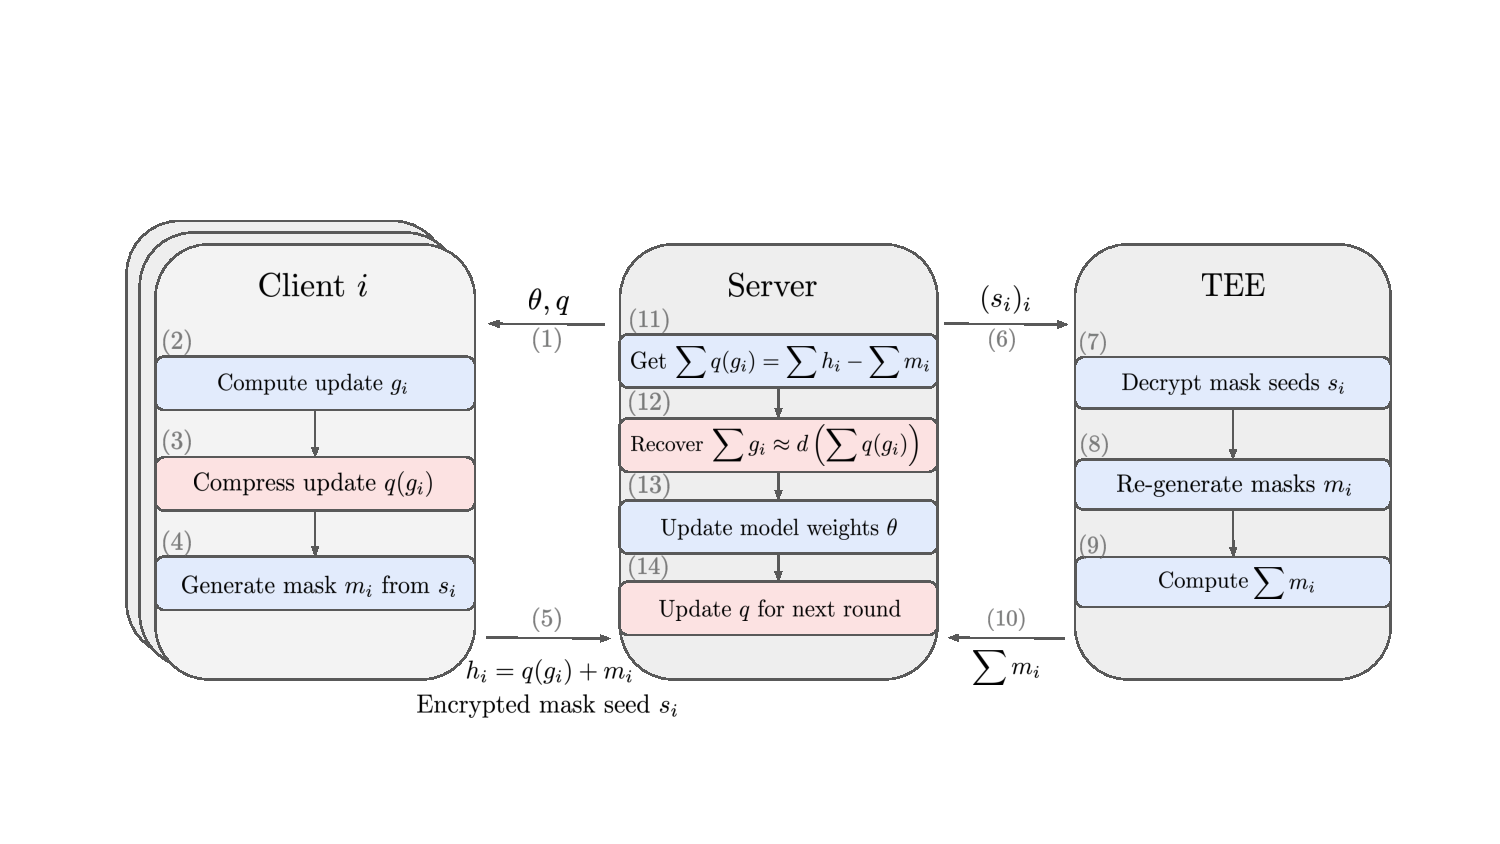
\includegraphics[width=0.8\textwidth]{figs/secagg_summary_new.pdf}
    %\vspace{-5mm}
    \caption{\label{fig:secagg_summary}
    Summary of the proposed approach for one FL round, where we omit the round dependency and \modif{Differential Privacy (DP)} for clarity. Blue boxes denote standard steps and red boxes denote additional steps for uplink compression. Client $i$ computes local model update $g_i$, compresses it with the compression operator $q$, and encrypts it by adding a random mask $m_i$ in the compressed domain, hence reducing the uplink bandwidth (steps 2--4). The server recovers the aggregate in the compressed domain by leveraging any \SecAgg protocol \modif{(steps 7--13, with a TEE-based \SecAgg, see Section~\ref{subsec:secagg})}. Since the decompression operator $d$ is linear, the server can convert the aggregate back to the non-compressed domain, up to compression error (step 12). As with the model weights $\theta$, the compression operator $q$ are also periodically updated and broadcast by the server (step 14). 
    In Section~\ref{sec:method}, we apply the proposed method to scalar quantization and pruning without impacting \SecAgg and propose Secure Indexing, a variant of \SecAgg for extreme uplink compression with product quantization. See Section~\ref{subsec:secagg} for details about \SecAgg and Section~\ref{sec:discussion} for a discussion on~DP.
    }
    \vspace{-3mm}
\end{figure*}



% Our focus in this paper is on 

%Second, scaling cross-device (synchronous) FL to millions of clients with various capabilities and intermittent availability \citep{bonavitz2019federated} suffers from diminishing returns: the wall-clock training time plateaus as the number of clients keeps increasing~\citep{huba2021papaya}. Even though this challenge can be addressed by leveraging the buffered asynchronous aggregation technique proposed by \cite{nguyen2021federated}, compatible with DP and SecAgg, the asynchronous protocol remains bottlenecked by communication latency between the server and the clients.


%Considering the above privacy and scalability goals, we focus on enabling efficient FL communications while keeping a high privacy bar. In addition to the primary objective of speeding up convergence, reducing communication costs brings other significant benefits. Lowering communication requirements addresses selection bias due to undersampling clients with limited connectivity, improving fairness and inclusivity metrics. Better communication efficiency shrinks the carbon footprint of FL, whose fraction attributable to communication can reach 95\%~\citep{qiu2021first}. %Finally, training larger model in FL would be a possibility, when the communication cost is reduced, because local memory or compute requirements can be addressed by modifying the local training loop, for instance with gradient checkpointing \citep{chen2016training}. However, some form of compression would be required to enable efficient communication.


%First, compressing model updates from the client to the server presents several challenges due to compatibility with SecAgg and is an area suitable for further research. 
%Second, upload bandwidth is generally more restricted than download. For instance, according to the most recent FCC report, the ratio of download to upload speeds for DSL/cable providers in the US ranges between 3$\times$ to 20$\times$~\citep{fcc-broadband}. We consider broadband speeds here because devices participate in the FL training while connected to fixed broadband, usually through Wi-Fi~\citep{huba2021papaya}.




% Hence, FL provides the ability to leverage data from massive client populations while ensuring the security and privacy of the client data.
% Go further: compatibility with DP / compression as a mitigation techniques of attacks
% Model and gradient compression intrinsically different.
%  Why not having the secure enclave perform the aggregation?
% \section{Requirements for a Multi-modal Data Science Platform}
\label{sec:requ-holist-data}

In this section we outline the requirements of a multi-modal data science platform and then introduce Vizier as a solution fulfilling these requirements. We start by discussing existing modalities that are widely used to interact with data in data science and their advantages and disadvantages. Converging on a set of modalities we deem to be essential, we then cover several cross-cutting concerns such as reproducibility and dealing with errors that are important no matter what modality is used to interact with data.

%%%%%%%%%%%%%%%%%%%%%%%%%%%%%%%%%%%%%%%%%%%%%%%%%%%%%%%%%%%%%%%%%%%%%%%%%%%%%%%%
\subsection{Modalities for Interacting with Data}
\label{sec:modal-inter-with}

Data scientists often employ several tools during the life-cycle of building a data pipelines. During data discovery, search engines (e.g., open data repositories) and dataset discovery tools (e.g., metadata management tools for data lakes) are used to identify data internal to an organization, data available for purchase, or openly available data that could be used to fulfill the goal the data scientist has in mind. The next step is typically to profile the data and understand its semantics and fitness for the task at hand. At this stage, data visualization is used, either in the form of specialized visualization systems or by employing visualization libraries written in, e.g., Python. This is often done from within notebook environments like Jupyter which can show visualizations inline with the users code. Afterwards, data is curated and integrated. Spreadsheets are often used for manual inspection of smaller datasets, repair of one-off errors, and to calculate basic statistics. Task-specific data cleaning systems or libraries written in a general purpose programming language are employed to (partially) automate this process. The cleaned and integrated data is then used in data analysis (e.g., building and evaluating machine learning models, running analytical queries, \ldots) and the final results of the analysis are visualized. Building a data pipeline is often an iterative process where the user revisits previous steps in the pipeline to deal with errors and to refine the processing.

%%%%%%%%%%%%%%%%%%%%%%%%%%%%%%%%%%%%%%%%%%%%%%%%%%%%%%%%%%%%%%%%%%%%%%%%%%%%%%%%
\subsubsection{Notebooks for Interactive Pipeline Development with Immediate Feedback}
\label{sec:noteb-inter-pipel}
%
Notebook systems like Jupyter and Apache Zeppelin to name just a few have become the quasi-standard for developing data science pipelines. One major advantage of notebooks is their highly interactive nature: users can run pieces of code and immediately observe their results. This makes it easy to debug steps in the pipeline and aids iterative development of pipelines. The outputs recorded in a notebook serve as a documentation of the data preparation and analysis process. Furthermore, most notebook system allow support documentation (typically written in a markup language such as markdown) to be interleaved with code. Even notebook interfaces have become prevalent, most existing implementations are suffer from poor reproducibility, do not support iterative development well, and are not suited well for large and complex pipelines. A recent study~\cite{PM19} on Jupyter notebooks collected from github observed that only 4\% of these notebooks are reproducibly in the sense that they can be rerun without errors and produce the same result as recorded in the notebook. We have argued in \cite{BS20, DG22} that these shortcomings are not inherent to the notebook model, but rather are the result of the architecture of notebook systems which use a long running kernel (e.g., a Python interpreter) and when the user runs a cell in a notebook send the cell's code to the kernel for execution. The kernels state, however, is hidden from the user and except for cell outputs is not encoded in the notebook itself. This leads to unreproducible behavior where the results recorded in the notebook no longer agree with a serial (top-down) execution of the notebook's cells. Furthermore, this can lead to stale results, if the user forgets to rerun cells whose code does dependent on the code in a cell that has been changed. Given the many benefits of and broad use of notebooks, support for a notebook interface is a must for any data science platform. We argue that by providing a notebook interface on top of a specialized workflow engine we can avoid the pitfalls of notebook systems which are thin wrappers around a kernel (Python interpreter). Specifically, we want a solution that supports a notebook interface (\textbf{requirement (N)} which fulfills the following conditions:
\begin{itemize}
\item \textbf{(N1) Serial Execution Semantics:} At any point in time, the results for the cells of the notebook agree with the results produced by a serial execution of the notebook.
\item \textbf{(N2) No Stale Outputs:} The outputs of each cell in the notebook should correctly reflect the current version of the notebook's code.
\item \textbf{(N3) Reproducibility:} The execution of a pipeline (notebook) does not depend on any hidden state. That is, as long as the code in the notebook is deterministic, rerunning a pipeline produces the same output as the original execution.
\end{itemize}

Note that any system that guarantees serial execution of notebooks as defined above, automatically guarantees that there are no stale outputs and that the execution of a notebook is reproducible.


%%%%%%%%%%%%%%%%%%%%%%%%%%%%%%%%%%%%%%%%%%%%%%%%%%%%%%%%%%%%%%%%%%%%%%%%%%%%%%%%
\subsubsection{Spreadsheets for Manual Curation and Exploration}
\label{sec:spre-manu-curat}
%
While notebooks are suited well for programmatic transformation and exploration of data, spreadsheet interfaces enable manual exploration and one-off transformations and fixes~\cite{FG16}. For instance, a user may search for and correct a few mistyped attributes values through a spreadsheet interface. Spreadsheets are also suited well for testing simple data transformations on a few rows using formulas and then once the transformation is satisfactory apply the transformation to a large number of rows by applying the same formula to many rows. Many spreadsheet systems have support for tracking changes made to the spreadsheet, but lack mechanisms to navigate the version history of a spreadsheet and to create branches, e.g., to try out a crazy idea without breaking a deployed version of a data science pipeline. As observed elsewhere~\cite{bendre-19-fhs}, spreadsheet systems do not typically scale to large datasets. While it is anyways infeasible to manually clean and curate large datasets, developing manual fixes on a sample / subset of a large dataset and then deploying the fixes to the dataset can be quite effective. Most spreadsheet systems use a data model that is incompatible with other structured data models such as the relational data model or data frames (which are essentially relations with row indexes) in that (i) columns do not have to be declared but are used by inserting a value into one cell of a column, (ii) the values of a column do not need to belong to a single datatype (e.g., some cells in a column may store strings while others are integers), and (iii) some operations  change the row and column positions rather than their content (e.g., inserting a row, changes the positions of all following rows). To support spreadsheets as a modality (\textbf{requirement (S)}, data science platforms should:
\begin{itemize}
\item \textbf{(S1) Translating between Relations and Spreadsheets:} It should be possible to manipulate standard relations through a spreadsheet view as well as process spreadsheets in other modalities.
\item \textbf{(S2) Supporting Spreadsheet Operations over Relations:} It should be possible to apply spreadsheet operations such as inserting / deleting rows / columns.
\item \textbf{(S3) Scalability:} It should be possible access large datasets through a spreadsheet interface.
\end{itemize}

%%%%%%%%%%%%%%%%%%%%%%%%%%%%%%%%%%%%%%%%%%%%%%%%%%%%%%%%%%%%%%%%%%%%%%%%%%%%%%%%
\subsubsection{Profiling and Interactive Visualizations}
\label{sec:inter-visu}
%
Data profiling and visualization are important tools for data scientists to explore data, understands its semantics, and identify problems with the data.
Data science platforms should support visualizations (\textbf{requirement (V)}). For example, a typical task in the initial data exploration phase of constructing a pipeline is to analyze and visualize the data distributions of columns in a dataset, e.g., by computing histograms for individual columns or by calculating the number of null values per column. Another common approach is to visualize correlations between columns. Both the spreadsheet and notebook modalities discussed so far, do support creation of plots and other data visualizations. Visualization recommendation~\cite{lee-21-l, hu-19-v} guide the user in exploring visualizations that help them to understand their data. A data science platform should support out-of-the-box visualizations  for common tasks (\textbf{requirement (V1)}, e.g., accessing data distributions as histograms as well as provide access to more general visualization tools (\textbf{requirement (V2)} to enable creation of custom visualization of, e.g., analysis results.

%%%%%%%%%%%%%%%%%%%%%%%%%%%%%%%%%%%%%%%%%%%%%%%%%%%%%%%%%%%%%%%%%%%%%%%%%%%%%%%%
\subsubsection{Semi-automated Data Cleaning, Curation, and Integration}
\label{sec:semi-automated-data}
%
As has been observed repeatedly in the past~\cite{nyt:wrangling}, data scientists spend the majority of their time in data discovery, preparation, and curation. Data cleaning, integration, and curation are complex tasks that are time consuming and error-prone. While full automation of these tasks is typically not an option, a plethora of semi-automated tools (e.g., constraint-based data cleaning~\cite{ilyas-15-tcrd}, schema matching~\cite{RB01}, and data integration~\cite{HR06}) which rely on heuristics and often involve the user in curation decisions have been proposed and exist in the form of stand-alone tools and libraries available for languages such as Python. Data science platforms should enable users to use such tools and algorithms in their data science pipelines (\textbf{requirement (C)}. Most approaches for automating data wrangling rely on heuristics to clean data. This is due to the fact that typically insufficient information is available to determine what the correct repair for a dataset is. For instance, when repairing a primary key constraint by tuple deletion~\cite{ilyas-15-tcrd}, one has to retain at most one tuple from each group of tuples with the same primary key value, however, we typically lack information to decide which tuple is the correct one to keep. Thus, data repair algorithms instead use heuristics such as preferring tuples with values that are common in the dataset or optimizing a global metric~\cite{RC17}. Data science platforms should track changes made based on heuristics and how they affect downstream operations as well as provide the user with an overview of what other choices did exist and how different choices would have affected the user's analysis results (\textbf{requirement (U)}):
\begin{itemize}
\item \textbf{(C) (Semi-)automated Data Curation and Integration:} Data science platforms should empower users to access (automated) data curation, cleaning, and integration techniques.
\item \textbf{(U) Tracking the Impact of Uncertain Choices:}  The impact of heuristic choices should be tracked through the operations in a data pipeline to aide the user in understanding how these choices have affected their analysis results and how the results would be affected if another alternative would have been chosen during data cleaning.
\end{itemize}

In summary, all modalities we have discussed so far have in common that they provide ways for the user to interact with data by applying transformations that create new data artifacts or update existing data artifacts and by viewing artifacts through user interfaces. For instance, plotting a histogram of the value distribution of an attribute in a csv file involves several transformations: (i) load the CSV file into a suitable in-memory data structure (e.g., a Pandas dataframe); (ii) aggregate the data to create a histogram; (iii) transform the histogram into a plot. We argue that it is feasible to build multiple modalities as ``views'' on top of a single dataflow platform. This approach has the advantage that the user does not have to to manually transform data between different formats expected by systems implementing the different modalities. Even more important, critical orthogonal functionality  such as versioning (that we will discuss next) has to only be implemented once.

%%%%%%%%%%%%%%%%%%%%%%%%%%%%%%%%%%%%%%%%%%%%%%%%%%%%%%%%%%%%%%%%%%%%%%%%%%%%%%%%
\subsection{Cross-cutting Concerns}
\label{sec:cross-cutt-conc}

Independent of which modality is used to interact with the data, there are important cross-cutting concerns such as reproducibility, supporting the user in iterative development of their data pipelines, dealing with data errors and uncertainty, and how to document data which need to be addressed. Some of the issues with implementing these cross-cutting functionality for specific modalities was already discussing in \Cref{sec:modal-inter-with}, but here we

\begin{itemize}
\item \textbf{(R) Reproducibility and Versioning:} Developing a data science pipeline typically requires several rounds of iterative development and refinement and may involve more than one developer. Keeping track of versions of the pipeline (and the associated results) in a version control manner is critical for aiding users in their development process (e.g., roll back to a past working version of the pipeline or test an experimental idea in a separate branch). However, we argue that unlike in version control systems where the user decides which versions of their code are persisted, for data science platforms it is beneficial if by default all past versions are retained (\textbf{requirement (R1)}). That is there should be no difference between the state kept for supporting undo as well as state kept for versioning. Furthermore, for reproducibility, unless the user's code contains non-deterministic operations, repeated executions of a pipeline should return the same result. Since we want to support interactive modalities like spreadsheets, modifications made through such modalities (e.g., manual edits of cell values or inserting and deleting rows in a spreadsheet) have to be translated into steps in the pipeline (\textbf{requirement (R2)}).
\item \textbf{(I) Supporting Iterative Refinement of Pipelines:} Data pipelines are typically constructed in an iterative fashion by adding additional steps and revisiting prior steps in the pipeline. For example, if an analysis returns unexpected results, the user may backtrack and modify steps in the pipeline which clean the data that is used in the analysis. A data science platform should support users in this process by (i) providing an overview of the structure of the pipeline to help the user to navigate between different parts of the pipeline (\textbf{requirement (O)}), (ii) by providing coarse-grained provenance to help the user identify which steps affected the data used by a pipeline step (\textbf{requirement (P)}), and (iii) ensure that outputs of pipeline steps are always up to date when upstream steps are modified. Note that the last requirement is the ``no stale outputs'' requirement (\textbf{requirement (N2)}) we have already discussed in \Cref{sec:noteb-inter-pipel}.
\item \textbf{(D) Documenting Data and Operations:} One advantage of notebook style interfaces is that they allow code and data to be documented using a markup language. For instance, a user may use this feature to document some insights into the semantics of their data or to explain why they selected a particular cleaning or learning technique. However, documentation in notebooks is associated with steps in the pipeline (cells in the notebook) rather than with pieces of data. While this type of documentation should be support (\textbf{requirement (D1)}), data documentation serves a wide range of purposes such as documenting data semantics (e.g., the year for a column storing dates as a month and day of the month), encoding information of how data was collected and processed, and recording information about issues with the data (e.g., a heart rate measurement is outside of the physically possible range). In \cite{kumari:2021:cidr:datasense} we argued that documentation pertaining to data is mission critical should be associated with the data (\textbf{requirement (D2)}) and should persist through operations (\textbf{requirement (D3)}). For instance, if the user annotated some values in a dataset with a note explaining that these values are suspicious, then aggregated summaries derived from the data should also be associated with these notes.
\item \textbf{(E) Dealing with Errors and Uncertainty:} Uncertainty and errors are prevalent in many application domains due to sensor, outliers~\cite{HA04}, and data entry errors, heuristics applied during data curation, integration~\cite{AS10, FK11b}, and cleaning~\cite{YM15, BS10a}, and misinterpretation of data semantics. Data science platforms should help users in identifying errors, should provide access to semi-automated (heuristic) methods for cleaning and curating data such as the data repair techniques~\cite{B19, ilyas-15-tcrd}. Furthermore, the platform should help the user to determine how choices made during cleaning (whether by a human or an algorithm) affect the results of analyzing the data.
\end{itemize}

In this section we have outlined a set of requirements, both to support specific modalities of interacting with data as well as general requirements that any system for building data science pipelines should support.


%%% Local Variables:
%%% mode: latex
%%% TeX-master: "../2022_IEEE_DEB_Vizier"
%%% End:

%!TEX root=../2022_IEEE_DEB_Vizier.tex

% %%%%%%%%%%%%%%%%%%%%%%%%%%%%%%%%%%%%%%%%
% \begin{figure}[t]
%   \centering
%   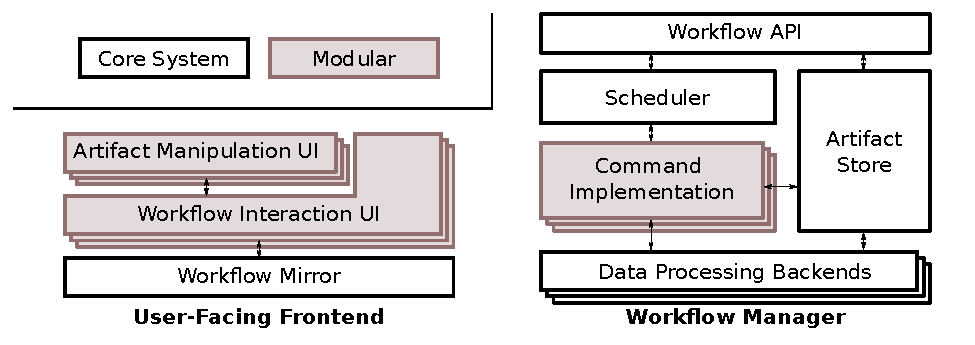
\includegraphics[width=0.7\textwidth]{graphics/systemarch}\\[-5mm]
%   \caption{Vizier's architecture, comprised of a user-facing frontend component and a backend component.}\label{fig:vizier-architecture}
% \end{figure}
% %%%%%%%%%%%%%%%%%%%%%%%%%%%%%%%%%%%%%%%%

%%%%%%%%%%%%%%%%%%%%%%%%%%%%%%%%%%%%%%%%%%%%%%%%%%%%%%%%%%%%%%%%%%%%%%%%%%%%%%%%
\pagebreak[4]
\subsection{Solution Overview}
\label{sec:solution-overview}

%%%%%%%%%%%%%%%%%%%%%%%%%%%%%%%%%%%%%%%%
\begin{wrapfigure}[12]{r}[0pt]{12cm}
  \centering
  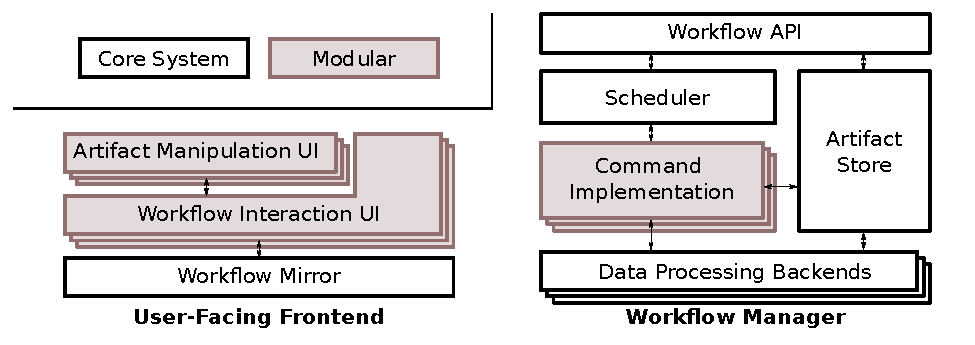
\includegraphics[width=0.7\textwidth]{graphics/systemarch}\\[-5mm]
  \caption{Vizier's architecture, comprised of a user-facing frontend component and a backend component.}\label{fig:vizier-architecture}
\end{wrapfigure}
%%%%%%%%%%%%%%%%%%%%%%%%%%%%%%%%%%%%%%%%
An overview of Vizier's architecture is shown in \Cref{fig:vizier-architecture}.
Addressing requirement \textbf{W1}, the central abstraction in Vizier is a workflow: a linear sequence of steps. % taken by the user in pursuit of a specific objective.
Unlike classical workflow systems, Vizier does not require users to explicitly declare information flow between steps.
Rather Vizier borrows the model employed in popular computational notebooks like Jupyter, where inter-cell communication occurs through a global state (artifacts) passed sequentially through steps.
Following notebook conventions, we refer to these steps as \emph{cells}, and the global state as a \emph{scope}, a map from artifact name to the version of the artifact valid at this point in the workflow. Vizier stores artifacts in common formats through a versioned \textbf{Artifact Store} (\Cref{sec:data-artifacts}), addressing requirement \textbf{A2}.
In \Cref{sec:vizier-workflows}, we formalize Vizier's workflow model, and show how we satisfy requirement \textbf{W3} by instrumenting how each cell interacts with the scope, allowing us to determine what artifact versions are valid.

Vizier's workflow semantics, paired with the versioned artifact store and workflow versioning (\Cref{sec:vizier-history}) addresses requirement \textbf{W2}. % as notebooks have a natural concept of logical order (the order of cells in the notebook) that can be adjusted over time.
% Adding workflow versioning  is sufficient to fully address the requirement.
In contrast, classical notebooks like Jupyter or Zeppelin rely on the global state of an interpreter for inter-cell communication.
Reverting this state to an earlier revision is challenging~\cite{zelnicki:2017:nodebook}, limiting their ability to satisfy requirement \textbf{W3}.
Vizier instead relies on its versioning system, allowing its \textbf{Scheduler} to automatically detect and re-evaluate stale cells (\Cref{sec:vizier-scheduler}).
To address requirement \textbf{A3}, we designed a light-weight uncertain data model that is implemented in Vizier in the form of \textit{caveats}, annotations on data that indicate uncertain values and rows  (\Cref{sec:data-docum-error}).

Addressing requirement \textbf{A1} requires modularity in both Vizier's front- and back-end components.
First, the user's interactions with a workflow and artifacts, whether through a scripting language, graphical interaction, or any other modality, need to be captured for replay (simultaneously addressing requirement \textbf{A4}). In Vizier this is achieved by requiring that every update to an artifact made through a particular modality has to be reflected as an operation in the workflow, i.e., a data update is translated into a workflow update.
Vizier manages a collection of \textbf{Command Implementations} that implement the logic behind these artifact transformations (\Cref{sec:multimodality}).
To streamline the implementation of commands, Vizier's data formats and transformations are built over standard \textbf{Data Processing Backends} like Apache Spark.
% For example, Vizier supports fine-grained provenance over datasets by encoding them as Spark data frames.

The frontend is implemented over a \textbf{Workflow Mirror} that uses websockets to reflect a live view of the workflow the user is editing.
Vizier automatically derives a default \textbf{Artifact Manipulation User Interface} for its notebook interface from each command's parameter schemas. This interface suffices for many templated commands, but the frontend can be further extended to provide a more customized experience, for example for Spreadsheet-style direct manipulation of data (\Cref{sec:spreadsheets}).
As illustrated in \Cref{fig:screenshot}, the frontend displays three \textbf{Workflow Interaction User Interfaces} by default: (i) A direct display of the workflow as a notebook, (ii) a table of contents summary of the notebook, including highlighting from documentation, and (iii) a list of artifacts derived by the notebook.
Several of these components, including the notebook and the artifact list provide access to direct manipulation interfaces.
Additional views currently implemented in Vizier include: (iv) A caveat view (\Cref{sec:data-docum-error}) that shows and tracks potential errors in the workflow and data, (v) a history view that shows the evolution of the workflow over time, and (vi) a data provenance subway diagram view.

%%%%%%%%%%%%%%%%%%%%%%%%%%%%%%%%%%%%%%%%%%%%%%%%%%%%%%%%%%%%%%%%%%%%%%%%%%%%%%%%
\begin{figure}
  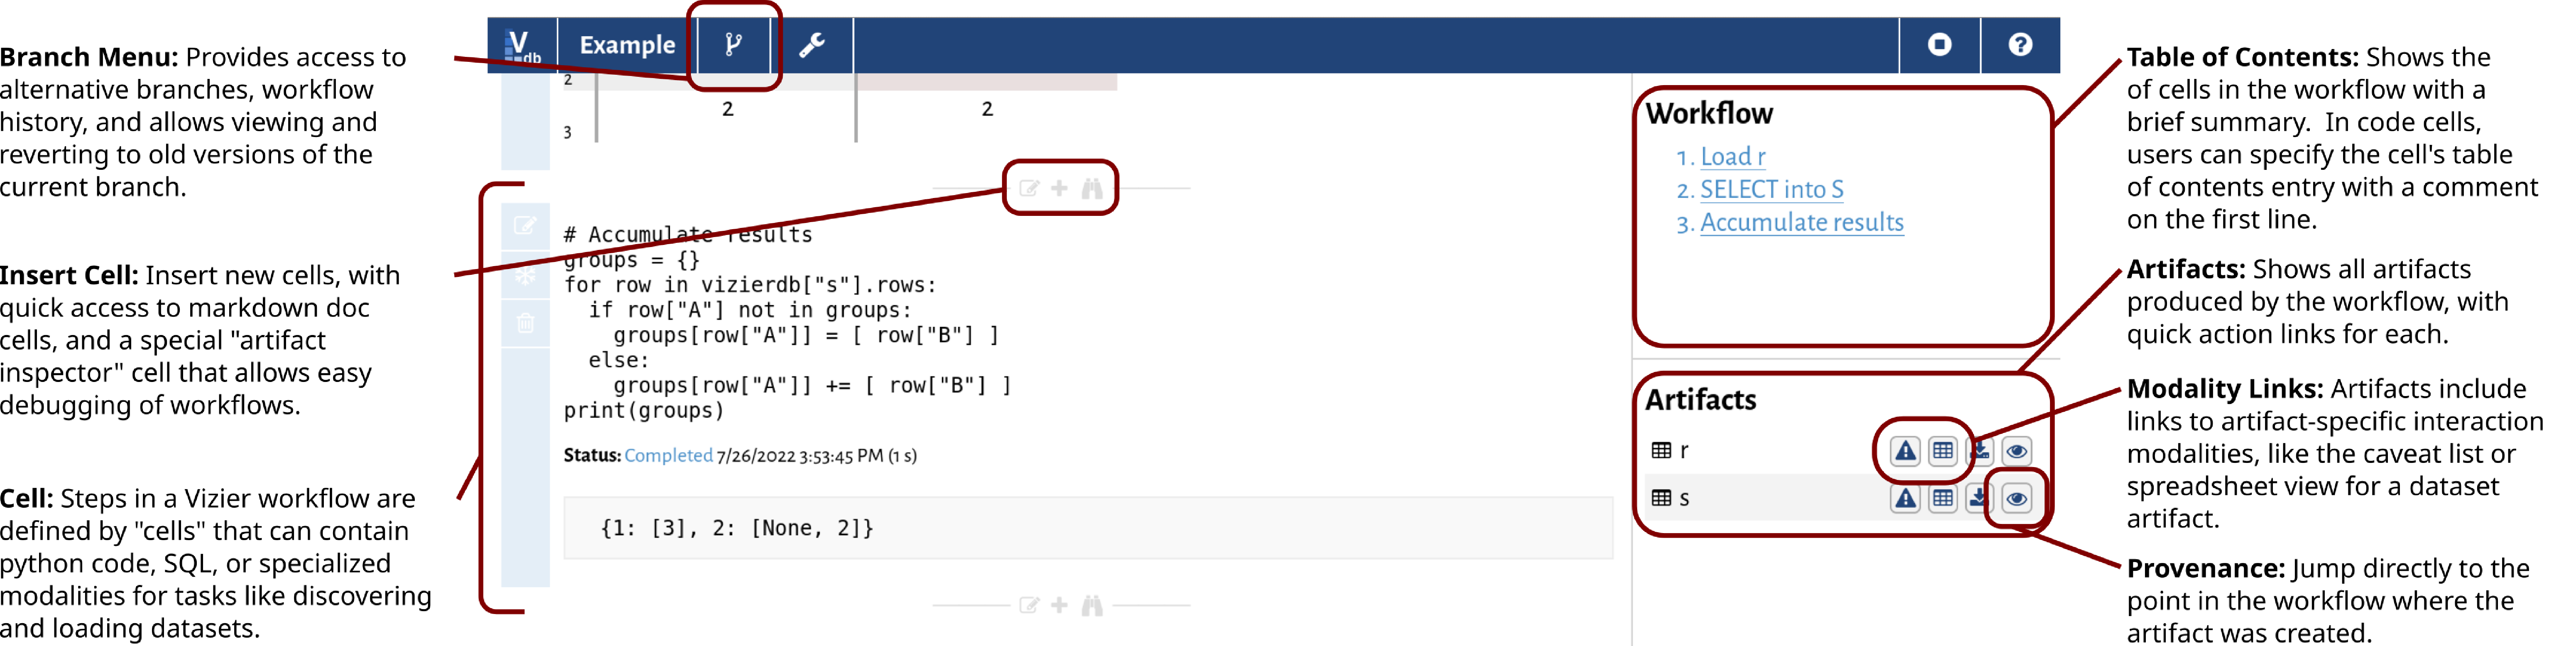
\includegraphics[width=\textwidth]{graphics/screenshot.pdf} 
  \caption{The Vizier User Interface}
  \label{fig:screenshot}
\end{figure}
%%%%%%%%%%%%%%%%%%%%%%%%%%%%%%%%%%%%%%%%%%%%%%%%%%%%%%%%%%%%%%%%%%%%%%%%%%%%%%%%

%%% Local Variables:
%%% mode: latex
%%% TeX-master: "../2022_IEEE_DEB_Vizier"
%%% End:

%!TEX root=../2022_IEEE_DEB_Vizier.tex
%%%%%%%%%%%%%%%%%%%%%%%%%%%%%%%%%%%%%%%%%%%%%%%%%%%%%%%%%%%%%%%%%%%%%%%%%%%%%%%%
\section{Versioned Data Artifact Store}
\label{sec:data-artifacts}

Steps in Vizier workflows create, read, and update \textit{``data artifacts''} or artifacts for short.
To maximize interoperability between cells, Vizier establishes standards for how these artifacts are serialized, which we now discuss. Versions of artifacts are immutable. 
An update to an artifact creates a new object representing the updated artifact. Immutability greatly simplifies handling of state in Vizier and enables us to share artifact versions across multiple revisions of a workflow.

\mypara{Dataset Artifacts}
Tabular data is represented by Vizier as a Spark dataframe~\cite{AX15}, a logical encoding of how a dataset is derived from source data.
The choice to store datasets through a logical representation (specifying the computation instead of its result) is driven largely by the need for managing annotations (requirement \textbf{A3} which is implemented by rewriting the computation to handle annotations), but also results in lower space consumption.
% Because data frames are not serializable, Vizier instead stores dataframe constructors: standardized logic for instantiating a data frame, e.g. by transforming or applying other artifacts.

% Vizier's dataframe constructors are a close analog of SparkML's \texttt{Pipeline}s, which provide a serializable representation of data frame transformation logic.
% Although Vizier provides a pipeline data frame constructor, Pipelines are strictly a representation of transformations, normally requiring glue code to apply the pipeline to an independently loaded dataset;
% Constructors completely capture the logic needed to instantiate a dataframe.

\mypara{Parameter Artifacts}
A parameter artifact can be any primitive value of any data type supported by Apache Spark; We note that this includes simple nested collections like Arrays and Maps.
This type of artifact provides a way to parameterize scripts and other system components, particularly for non-technical users.
% Vizier provides a ``Set Parameter'' command that allows users to specify parameters;
and parameter artifacts are used to pass simple data (e.g., simple constants in Python) between cells.

In addition to these two artifact types, Vizier also supports plots (stored in the vegalite~ \cite{DBLP:journals/tvcg/SatyanarayanMWH17} format), blobs and uninterpreted files, and language-specific constructs, e.g., Python function definitions. For lack of space, we do not further  discuss these other artifact types.

% \mypara{Chart Artifacts}
% Although Vizier provides means for plot generation (e.g., Bokeh, Matplotlib) through messages emitted by a cell, a standardized vegalite~\cite{DBLP:journals/tvcg/SatyanarayanMWH17} artifact format allows multiple cells to collaboratively edit a plot.
% For example, a ``Chart'' command makes it easy for users to quickly visualize a dataset, and then a Spark or Python cell can refine the resulting visualization by tweaking labels, adding markers, or adjusting colors.

% \mypara{Blob and File Artifacts}
% As a fallback to other data formats, Vizier allows cells to export state through a simple blob format.
% For example, Python falls back to encoding global state in `pickle' format, which is stored as a simple blob.
% The blob store is encoded as an in-memory array; If the artifact is large enough to warrant disk IO (e.g., a large model), requires a directory structure (e.g., parquet files), or is otherwise tied to the filesystem, Vizier provide a file artifact format.
% File artifacts are stored in a unique location tied to the artifact identifier.

% \mypara{Function Artifacts}
% Symbols representing language-specific constructs like functions, classes, and imported modules are encoded as raw code.
% Each artifact stores condains code that defines a single symbol under a specific name.
% At time of writing, support for function artifacts requires explicit cross-platform implementation support, although efforts are under way to provide a standardized cross-language interface.




%%% Local Variables:
%%% mode: latex
%%% TeX-master: "../2022_IEEE_DEB_Vizier"
%%% End:

% %!TEX root=../2022_IEEE_DEB_Vizier.tex
\section{Microkernel Notebooks}
As we outline above, a typical computational notebook relies on a kernel, a long-lived interpreter for a scripting language for a scripting language like python that retains the notebook's intermediate state.
When a cell is executed by the user, its contents are evaluated by the long running interpreter; the interpreter's state changes, and any output produced by the cell (e.g., console logs, charts, or maps) is displayed alongside the cell.
This behavior is independent of the order in which the cell appears in the notebook: The user may return to an earlier cell and modify it, but this cell is simply run against the current state of the interpreter.

Although this design allows users to revise cells in the notebook without being forced to re-run all of the notebooks code from scratch, it does pose several problems.
Most notably that it forces users to reason about the internal state of the kernel, for example by manually adopting a single static assignment variable allocation pattern.
Second, it also requires users to manually keep track of how different notebook cells relate to one-another; When a cell is modified, other cells that depend on it may also need revision.
Finally, in this design, persistence (e.g., of the results of a slow-running computation) must be managed entirely by the user.
Moreover, it is up to the user to manually manage this state to ensure consistent versioning, and portability.

One class of systems including Vizier~\cite{BS20,BB19} and Nodebook address these challenges by checkpointing global notebook state in between cell executions and restoring it when a cell is re-executed.
Thus, the cell is always evaluated on the state version emitted by the preceding cell, and changes to the state can be identified so that subsequent cells that depend on modified outputs can be re-evaluated.
This model 


\begin{itemize}
	\item Standard API for interacting with notebook state facilitates multi-modality
	\begin{itemize}
		\item No $N^2$ problem like for jupyter kernels
		\item Not just notebooks
	\end{itemize}
	\item Typed API allows fine-grained provenance
	\begin{itemize}
		\item Reproducibility
		\item Automatic refresh
		\item No hidden (mystical) dependencies
	\end{itemize}
	\item Challenges:
	\begin{itemize}
		\item Communicating state between kernels
		\item 2-dimensional version model (cell-order vs historical-order <- better name for this exists)
		\item Input/output changes in history vs Operation changes in history
		\begin{itemize}
			\item Vizier: Module vs Cell vs Result
			\item The Vizier execution state-model
		\end{itemize}
		\item Scheduling / Deciding state
	\end{itemize}
\end{itemize}

%%% Local Variables:
%%% mode: latex
%%% TeX-master: "../2022_IEEE_DEB_Vizier"
%%% End:

%!TEX root=../2022_IEEE_DEB_Vizier.tex
\section{Workflow Provenance Model and Runtime}
\label{sec:vizier-workflows}

In this section, we outline Vizier's workflow and versioning model, how we determine which cells of a workflow need to be re-executed if a cell is changed, and introduce the parallel scheduler of the system.

% multi-tiered, two-dimensional provenance model.
% We first relate the model to both classical workflow provenance and modern computational notebooks, then discuss how Vizier's model incorporates a temporal dimension, and finally discuss state invalidation and re-evaluation.

\newcommand{\notebook}{\mathcal N}
\newcommand{\workflow}{\mathcal W}
\newcommand{\artifact}{a}
\newcommand{\nbcell}{c}
\newcommand{\outputval}{o}
\newcommand{\readset}{\vec r}
\newcommand{\writeset}{\vec w}
\newcommand{\globalscope}{\mathcal G}
\newcommand{\outputdomain}{\mathcal O}
\newcommand{\valuedomain}{\mathcal D}
\newcommand{\undefinedval}{\bot}
\newcommand{\unknownval}{\circledcirc}
\newcommand{\keyset}{\texttt{keys}}
\newcommand{\changeset}{\Delta}
\newcommand{\variabledomain}{\Sigma}
\newcommand{\diff}[2]{\Delta(#1, #2)}
\newcommand{\evalnb}[1]{\llbracket #1 \rrbracket}

\begin{figure}
  \centering
  \begin{minipage}{0.9\textwidth}
  \begin{lstlisting}[style=pynotebook]
data = read_csv("social_data.csv")
show(data)
  \end{lstlisting}

  \begin{lstlisting}[style=pynotebook]
data["latlon"] = geocode(data["address"])
show(data)
  \end{lstlisting}

  \begin{lstlisting}[style=pynotebook]
censusblocks = read_geojson("blocks.json")
show(censusblocks)
  \end{lstlisting}

  \begin{lstlisting}[style=pynotebook]
data = spatial_join(data, censusblocks, ["latlon", "geometry"])
count_per_block = data.groupby("block_id").count()
show(count_per_block)
  \end{lstlisting}
  \end{minipage}\\[-4mm]
  \caption{A simplified example notebook}
  \label{fig:exampleNotebook}
\end{figure}

%%%%%%%%%%%%%%%%%%%%%%%%%%%%%%%%%%%%%%%%%%%%%%%%%%%%%%%%%%%%%%%%%%%%%%%%%%%%
%%%%%%%%%%%%%%%%%%%%%%%%%%%%%%%%%%%%%%%%%%%%%%%%%%%%%%%%%%%%%%%%%%%%%%%%%%%%
\subsection{Workflow Model}
\label{sec:vizier:eval}

A workflow in Vizier is a sequence of workflow steps (cells) that can read and write artifacts. 
Artifacts are versioned at the granularity of cells. 
A cell writing an artifact $\artifact$ causes a new version of $\artifact$ to be created. 
We will discuss the APIs Vizier exposes to the data interaction modalities for accessing artifacts in \Cref{sec:multimodality}. 
The semantics of a Vizier workflow is the serial execution of the cells of the workflow, where the latest version of each artifact is passed as input to the cell that will be executed next. 
Thus, as long as the cells themselves are deterministic, the artifact versions created by the execution of a workflow are uniquely determined by the workflow itself.

%%%%%%%%%%%%%%%%%%%%%%%%%%%%%%%%%%%%%%%%%%%%%%%%%%%%%%%%%%%%%%%%%%%%%%%%%%%%%%%%
\begin{exam}
  \label{ex:introduction}
  \Cref{fig:exampleNotebook} shows a notebook with a simplified data ingestion, cleaning, and analysis task.
  The notebook loads the dataset (cell 1), geocodes listed street addresses (cell 2), loads a collection of census blocks (cell 3), and computes summary statistics for each census block (cell 4).
  We use this  notebook to illustrate a key challenge of traditional  notebook architectures.
  %
  The user modifies cell 2 to switch to a different geocoder, potentially requiring re-evaluation of the notebook.
  In this specific notebook, the user had the foresight to write in an idempotent style, making it unnecessary to re-run cell 1 to recover the state needed to run cell 2 correctly.
  It is also unnecessary to re-run cell 3, as it does not depend on the output of cell 2.
  However, in traditional notebooks like Jupyter the burden of deciding which cells to re-evaluate rests on the user, creating added overhead and increasing the chance of errors.
\end{exam}
%%%%%%%%%%%%%%%%%%%%%%%%%%%%%%%%%%%%%%%%%%%%%%%%%%%%%%%%%%%%%%%%%%%%%%%%%%%%%%%%

Formally, a Vizier workflow is a sequence $\notebook = \{ \nbcell_1, \ldots, \nbcell_N \}$ of cells. 
The versions of artifacts valid after execution of cell $\nbcell_i$ are modeled as a global scope $\globalscope$ that maps artifact names to artifact versions or the distinguished symbol $\undefinedval$, which indicates that no version of the artifact has been produced yet.  
A cell $\nbcell$ is a function that takes a scope $\globalscope$ as input and produces an updated scope $\globalscope'$: $\nbcell (\globalscope) = \globalscope'$. 
We use $\readset_{\globalscope,i}$ to denote the names of artifacts accessed by cell $\nbcell_i$ applied to $\globalscope_i$. 
The scope parameter is necessary, because a cell may dynamically decide which artifacts to read based on the content of other artifacts.
%
The result $\evalnb{\notebook}$ of  evaluating workflow $\notebook = \{ \nbcell_1, \ldots, \nbcell_N \}$ is defined as the scope $\globalscope_n$ produced by starting with an empty scope $\globalscope_0$ (where all artifact names are mapped to $\undefinedval$), and by computing $\globalscope_{i} = \nbcell_{i}(\globalscope_{i-1})$.








% Cell evaluation in Vizier happens in notebook-order.

% Each cell is (conceptually) evaluated on the scope emitted by the preceding cell.
% Like the workflow systems that inspired it, Vizier retains inter-cell snapshots of scope to preserve notebook-order evaluation semantics while still allowing users to backtrack.


% Denote by $\globalscope$ a global scope that we will formalize shortly;

% We model a cell $\nbcell (\globalscope) = (\globalscope', \readset, \outputval)$ as a deterministic function applied to a global scope that returns a new global scope $\globalscope'$, a read set $\readset$, and an opaque output object $\outputval$ in $\outputdomain$.
% Evaluating the notebook $\evalnb{\notebook} = (\globalscope_N, [\outputval_1, \ldots, \outputval_N)$ produces a final scope $\globalscope_N$ and a sequence of outputs $\outputval_1, \ldots, \outputval_N$ through straightforward composition, starting with an empty scope $\globalscope_0$.
% %  formalized as:
% % $$(\globalscope_i, \readset_i, \outputval_i) = \nbcell_i(\globalscope_{i-1})$$
% % In the above,

%%%%%%%%%%%%%%%%%%%%%%%%%%%%%%%%%%%%%%%%
\begin{wrapfigure}[8]{r}[0pt]{11cm}
  \centering
  \vspace{-4mm}
  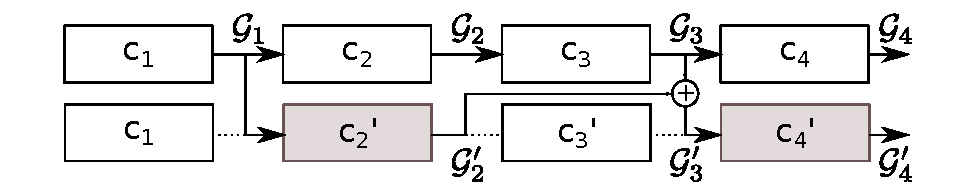
\includegraphics[width=10.5cm]{graphics/eval.pdf}\\[-5mm]
  \caption{Evaluation logic for the example notebook in \Cref{fig:exampleNotebook}.  Edges are labeled with global scope versions.  Cells that are (re-)evaluated are highlighted, dotted lines represent simulated state flow.}
  \label{fig:exampleEval}
\end{wrapfigure}
%%%%%%%%%%%%%%%%%%%%%%%%%%%%%%%%%%%%%%%%
If workflow $\notebook$ is modified by replacing a cell $\nbcell_i$ with a cell $\nbcell_i'$ (denoted as $\notebook[\nbcell_i \backslash \nbcell_i']$), we need to obtain the updated scope $\evalnb{\notebook[\nbcell_i \backslash \nbcell_i']}$. Of course this can be achieved by evaluating $\notebook[\nbcell_i \backslash \nbcell_i']$.
% In lieu of naively re-evaluating the notebook from scratch,
However, to improve performance,  Vizier attempts to update the output of $\evalnb{\notebook}$ by only re-evaluating a subset of the cells.
First, observe that $\globalscope_1, \ldots, \globalscope_{i-1}$ are independent of $\nbcell_i$; and remain unchanged if $\nbcell_i$ is modified.
It is still necessary to have $\globalscope_{i-1}$ to evaluate $\nbcell_i'$; so Vizier caches all intermediate global scopes after evaluating each workflow revision.

% \begin{figure}
%   \centering
%   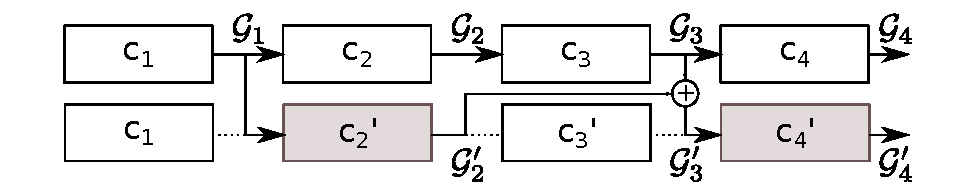
\includegraphics[width=0.7\textwidth]{graphics/eval.pdf}
%   \caption{Evaluation logic for the example notebook in \Cref{fig:exampleNotebook}.  Edges are labeled with global scope versions.  Cells that are (re-)evaluated are highlighted, dotted lines represent simulated state flow.}
%   \label{fig:exampleEval}
% \end{figure}

Naively, we have to still re-evaluate $\nbcell_{i+1}, \ldots, \nbcell_{N}$ using the new scope produced by $\nbcell_i'$. Let us denote the scopes produced by this evaluation as
$\globalscope_{i+1}', \ldots, \globalscope_{n}$.
% $\outputval_{i+1}', \ldots, \outputval_{N}'$.
Vizier uses the readsets $\readset_{\globalscope, i+1}, \ldots, \readset_{\globalscope, N}$, to identify cells $\nbcell_{j}$ for which the same output (artifact versions written by the cell) in $\evalnb{\notebook[\nbcell_i \backslash \nbcell_i']}$ is guaranteed. 
Denote by $\changeset(\globalscope, \globalscope') = \{ k |  \globalscope(k) \neq \globalscope'(k)\}$ the names of artifacts that differ between $\globalscope$ and $\globalscope'$. 
We have to re-execute cell $\nbcell_{i+1}$ if an artifact read by $\nbcell_{i+1}$ has changed, which is the case if $\changeset(\globalscope_i, \globalscope_i') \cap \readset_{\globalscope,i+1} \neq \emptyset$. If $\nbcell_{i+1}$ needs to be re-executed, then we set $\globalscope_{i+1}' = \nbcell_{i+1}(\globalscope_{i}')$. Otherwise, we generate $\globalscope_{i+1}$ by merging the changes made by $\nbcell_{i+1}$ in $\notebook$ to $\globalscope_{i}$ into $\globalscope_{i}'$. That is, for all artifacts $k$ we set
$\globalscope_{i+1}'(k) =   \globalscope_{i+1}(k)$ if $k \in \changeset(\globalscope_i, \globalscope_{i+1})$
and $\globalscope_{i+1}'(k) = \globalscope_{i}'(k)$ otherwise.
% begin{cases}
%   \globalscope_{i+1}(k) &\;\;\;\text{\textbf{if}}\,k \in \changeset(\globalscope_i, \globalscope_{i+1})\\
%   \globalscope_{i}'(k) &\;\;\;\text{\textbf{otherwise}}\\
% \end{cases}$$
 The same approach is applied to decide whether to evaluate or skip the remaining cells in $\notebook[\nbcell_i \backslash {\nbcell_i}']$.


% We formalize a global scope $\globalscope = \{ k_1 \rightarrow v_1, k_2 \rightarrow v_2, \ldots \}$ as a total mapping from an infinite alphabet of variable names $k \in \variabledomain$ to a set of domain values $v \in \valuedomain \cup \{\undefinedval\}$.
% The distinguished symbol $\undefinedval$ denotes an ``undefined'' value, and we assume that finitely many elements of $\variabledomain$ are mapped to non-$\undefinedval$ values (i.e., that $\globalscope$ has finite support).
% Denote by $\keyset(\globalscope) = \{ k | (k \rightarrow v) \in \writeset \wedge v \neq \undefinedval\}$ the keys of the finite support of $\globalscope$.
% Denote by $\changeset(\globalscope, \globalscope') = \{ k |  \globalscope(k) \neq \globalscope'\}$ the change set between $\globalscope$ and $\globalscope'$.

% Given the newly computed $\globalscope_i'$, we want to know if $\nbcell_{i+1}$ needs to be evaluated as well;
% If $\nbcell_{i+1}(\globalscope_i') = (\globalscope_{i+1}', \readset_{i+1}', \outputval_{i+1}')$, we can avoid re-evaluating $\nbcell_{i+1}$ if we can prove that $\outputval_{i+1} = \outputval_{i+1}'$.
% Under the assumption that $\nbcell_{i+1}$ is deterministic with respect to inputs $\readset_{i+1}$, we can guarantee that $\outputval_{i+1} = \outputval_{i+1}'$ when $\readset_{i+1} \cap \changeset(\globalscope_{i}, \globalscope_{i}')$ is empty.
% If we do not need to re-evaluate $\nbcell_{i+1}$, we can reconstruct its output by considering how the original evaluation affected the scope: the write set $\writeset_{i+1} = \changeset(\globalscope_{i}, \globalscope_{i+1})$.
% Concretely $\outputval_{i+1}' = \outputval_{i+1}$, $\readset_{i+1}' = \readset_{i+1}$ and
% $$\globalscope_{i+1}'(k) = \begin{cases}
% \globalscope_{i+1}(k) \textbf{ if } k \in \writeset_{i+1}\\
% \globalscope_{i}'(k) \textbf{ otherwise}
% \end{cases}$$
% \noindent The remaining cells of the notebook are processed in a like manner.

 %%%%%%%%%%%%%%%%%%%%%%%%%%%%%%%%%%%%%%%%%%%%%%%%%%%%%%%%%%%%%%%%%%%%%%%%%%%%%%%%
\begin{exam}
  \Cref{fig:exampleEval} continues the running example from \Cref{ex:introduction}.
  The user has replaced the initial version of cell $\nbcell_2$ with an updated version ${\nbcell_2}'$.
  The global scope produced by preceding cells ($\globalscope_1$) may be re-used unchanged to evaluate ${\nbcell_2}'$, producing scope $\globalscope_2'$.
  $\changeset(\globalscope_2, \globalscope_2')$ is the \lstinline{data} artifact, but the readset of $\nbcell_3$ is empty, and so this cell does not need to be re-evaluated.
  Instead $\globalscope_3'$ is derived by merging variables the cell previously changed (i.e., $\changeset(\globalscope_2, \globalscope_3)$) into the current global scope.
  Finally, Vizier identifies that an element of $\readset_{\globalscope,4}$ (the \lstinline{data} variable) has changed between $\globalscope_3$ and $\globalscope_3'$, necessitating a re-evaluation of cell 4.
\end{exam}
 %%%%%%%%%%%%%%%%%%%%%%%%%%%%%%%%%%%%%%%%%%%%%%%%%%%%%%%%%%%%%%%%%%%%%%%%%%%%%%%%

% \mypara{Frozen Cells}
% Vizier allows users to ``freeze'' cells, temporarily replacing them with no-op commands, but preserving all user-interface elements (including cell outputs), and allowing the cell to be easily re-inserted into the notebook.
% This allows users to quickly disable cells with transient purposes (e.g., sampling cells), or avoid triggering expensive computations while working on an earlier part of the notebook.

% \begin{figure}
%   \centering
%   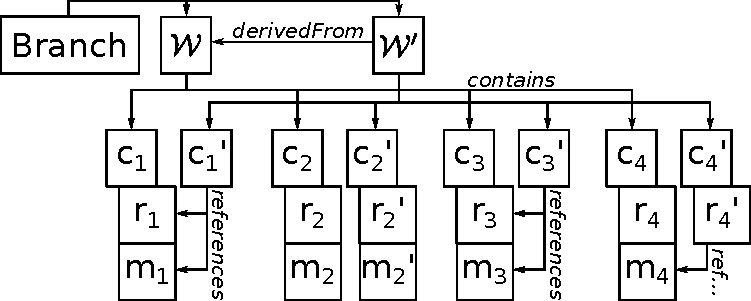
\includegraphics[width=0.45\textwidth]{graphics/history.pdf}\\[-3mm]
%   \caption{History for the running example, assuming cell B was changed as in \Cref{fig:exampleEval}.}
%   \label{fig:exampleHistory}
% \end{figure}

%%%%%%%%%%%%%%%%%%%%%%%%%%%%%%%%%%%%%%%%%%%%%%%%%%%%%%%%%%%%%%%%%%%%%%%%%%%%
%%%%%%%%%%%%%%%%%%%%%%%%%%%%%%%%%%%%%%%%%%%%%%%%%%%%%%%%%%%%%%%%%%%%%%%%%%%%
\subsection{Versioning Workflows}
\label{sec:vizier-history}

%%%%%%%%%%%%%%%%%%%%%%%%%%%%%%%%%%%%%%%%
\begin{wrapfigure}[10]{r}[0pt]{8cm}
  \centering
  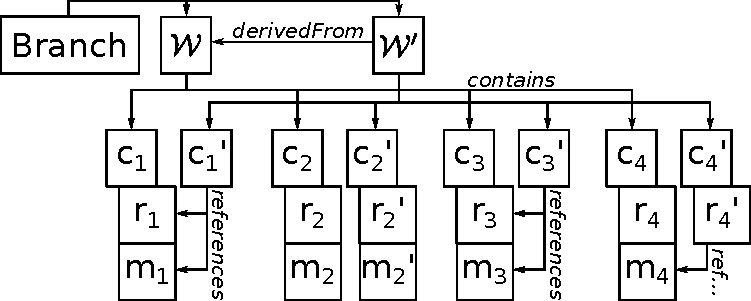
\includegraphics[width=0.45\textwidth]{graphics/history.pdf}\\[-3mm]
  \caption{History for the running example, assuming cell 2 was changed as in \Cref{fig:exampleEval}.}
  \label{fig:exampleHistory}
\end{wrapfigure}
%%%%%%%%%%%%%%%%%%%%%%%%%%%%%%%%%%%%%%%%
Vizier maintains a branching history of the evolution of the notebook.
% We use the term workflow ($\workflow = c_1, \ldots, c_N$) to denote a single state of the notebook.
A cell is further subdivided into (i) \textbf{cell metadata} ($c_i$) that is unique to the workflow (e.g., timestamps and execution status), (ii) \textbf{results} ($r_i$) of executing the cell, and (iii) a \textbf{module} ($m_i$) describing the command executed in the cell.
The latter two components (results and modules) may be shared across workflows.
% In other words, a single cell object acts as a many-to-many-to-many (i.e., 3-ary) relationship between workflow, module, and result entities.
A module object describes the command to be evaluated in a cell.  
This includes its type (e.g., Python or Scala script; SQL query; or one of the graphical widgets), as well as any parameters to the command (e.g., the script itself, or the artifact name to materialize query results as). 
A results object stores references to versions of artifacts in the artifact store created by the execution of the cell. 
We do not materialize the full global scope after each cell, but rather only the changes made to the global scope by the cell (i.e., the cell's write set). 
Any global scope $\globalscope_i$ can be reconstructed from the preceding write sets.

% A results object consists of three items: (i) Messages output by the cell (i.e., $\outputval$), (ii) The cell's readset as a list of name/artifact pairs, and (iii) The cell's writeset as a list of name/artifact pairs.
% Deletion is encoded by writing the distinguished value \texttt{null} to a name.
% As a performance optimization, name/artifact pairs do not embed the artifact literal, but rather a unique artifact identifier.
% This allows for efficient equivalence testing, while avoiding duplication; For example, a ``copy artifact" instruction only needs to clone the artifact identifier under a new name, and not the entire artifact.

% \mypara{Global scope}
% Note that the organizational structure used to persist history information differs from the global scope model used to reason about cell re-use.
% However, the two representations are equivalent.
% Denote by $m_1 \circ m_2$ the right-preferenced composition of \emph{partial} maps $m_1$ and $m_2$ as follows:
% $$m_1 \circ m_2 = \{ k\rightarrow v | (k \rightarrow v) \in m_1 \wedge \not\exists v' \text{ s.t. } (k \rightarrow v') \in m_2 \} \cup m_2$$
% Any global scope $\globalscope_N$ can be recovered by composing the preceding writesets: $\globalscope_N = \globalscope_0 \circ \writeset_1 \circ \ldots \circ \writeset_N$


\begin{exam}
 \Cref{fig:exampleHistory} continues our running example, which in our new terminology is a single branch comprised of two workflows $\workflow_1$ and $\workflow_2$.
  Both notebooks are comprised of four cell objects each.
  Cells 1, 3, and 4 were unchanged between workflows, and so the corresponding cell objects for $\workflow_2$ reference the same module description object as the corresponding cell for $\workflow_1$, while the module descriptions referenced by $\nbcell_2$ and ${\nbcell_2}'$ differ.
  Cells 1 and 3 do not need to be re-evaluated, and so can share their result objects, while Cells 2 and 4 both require re-evaluation and create new result objects.
\end{exam}

%%%%%%%%%%%%%%%%%%%%%%%%%%%%%%%%%%%%%%%%%%%%%%%%%%%%%%%%%%%%%%%%%%%%%%%%%%%%%%%%
\mypara{Workflow and Branch History}
Similar to version control systems like git, each workflow version in Vizier stores a reference to the workflow version it was derived from.
% The difference between workflow versions can be computed by comparing the sequence of modules referenced by the workflow's cells; but simple summary information including the type of change (insert, delete, update) and the affected module (if appropriate) is cached with the workflow object.
A branch is an append-only sequence of workflow versions. % with associated metadata (e.g., a branch name).
The branch contains a reference to the most recent workflow version in the branch. % prior versions are tracked through the series of derived-from references in the workflows themselves.
A new branch may be created from any existing workflow version, including a historical one.

%%%%%%%%%%%%%%%%%%%%%%%%%%%%%%%%%%%%%%%%%%%%%%%%%%%%%%%%%%%%%%%%%%%%%%%%%%%%
%%%%%%%%%%%%%%%%%%%%%%%%%%%%%%%%%%%%%%%%%%%%%%%%%%%%%%%%%%%%%%%%%%%%%%%%%%%%
\subsection{Parallel Scheduler}\label{sec:vizier-scheduler}

The evaluation model presented in \Cref{sec:vizier:eval} relies exclusively on \textit{dynamic provenance}, where Vizier is informed about the readset and writeset of a cell at runtime when the cell accesses artifacts through Vizier's API.
% that assist in determining whether a cell needs to be re-evaluated.
However, dynamic provenance is not always sufficient.
For example, Vizier evaluates cells in parallel where possible, but dynamic provenance is not available until the cell has already been evaluated.
Static provenance, which can derive a cell's read and write sets through static dataflow analysis of its source code, can be computed upfront.
However, static dataflow analysis is of necessity an approximation for some cell types; language features like control flow and dynamic code evaluation can lead to over- (or under-) estimates of the cell's read and write sets. % , especially with respect to a specific global scope.
Vizier uses a novel approach which refines static provenance at runtime using dynamic provenance~\cite{DG22}.

Fundamentally, Vizier's scheduler needs to assign each cell in a running workflow to one of four lifecycle stages: (i) \textbf{DONE} when the cell has a valid result object, (ii) \textbf{PENDING} when the cell depends (directly or transitively) on a cell that does not have a result object, and (iii) \textbf{RUNNING} when the cell's dependencies have a valid result object but the cell itself does not.
We further distinguish as (iv) \textbf{STALE} those cells in the \textbf{PENDING} stage for which we can conclusively determine that re-evaluation is required.
% Lifecycle stage transitions are monotonic.

To manage lifecycle transitions, Vizier's scheduler relies on a combination of static and dynamic provenance~\cite{DG22}.
It uses static provenance to generate an over-approximation on the read and write dependencies of a cell\footnote{As we argue in~\cite{DG22}, to deal with languages that support dynamic code evaluation such as Python, it would be necessary to allow under-approximations of read and write sets (missed data dependencies) and compensate for them at runtime. However, this not implemented in Vizier yet; attempts to dynamically read variables not in the maximal readset are flagged as errors.}.
  % Vizier does not presently support purely dynamic dependencies through e.g., dynamic code evaluation.  A read or write access on a variable not discovered through static analysis triggers an execution error.}.
Accordingly, the scheduler tracks an over-approximation of the read and writesets at each step of the workflow, and refines them when the execution of cell finishes and we know its precise read and write set. 
This approximation is used by Vizier's scheduler to omit cells from re-execution or schedule them for parallel execution if we can determine that it is safe to do so based on these over-approximations.

% Approximate global scopes generalize our prior definition of a global scope by extending the value domain to include the value $\unknownval$, denoting an unresolved value (i.e. variables in an approximate global scope are drawn from $\valuedomain \cup \{\undefinedval, \unknownval\}$).
% Like a regular global scope, an approximate global scope is derived by concatenating writesets ($\globalscope_i = \globalscope_{i-1} \circ \writeset_i$).
% However, if the cell is in a lifecycle stage other than \textbf{DONE}, its previous writeset is not valid.
% Instead, Vizier uses static analysis to derive an upper bound on the writeset $\writeset_{\max} \subseteq \variabledomain$, the maximal set of variables that the cell is allowed to write to.
% When the cell's writeset is not (or may not be) valid, the approximate global scope is instead updated by making each element of $\writeset_{\max}$ an unknown:
% $\globalscope_{i} = \globalscope_{i-1} \circ \{ k \rightarrow \unknownval | k \in \writeset_{\max, i} \}$

% \Cref{alg:lifecycleStage} explains how Vizier derives the lifecycle stage of a cell from the global scope emitted by the preceding cell, the cell's readset (if it exists), and the bound on the readset derived from static analysis.
% The first consideration is whether the cell's prior result object is still valid.
% If there is no prior result object (e.g., because the cell is newly inserted), or if the prior result object is definitely invalid (i.e., because a previously read value was definitely overwritten by a re-evaluated cell), the cell must be re-evaluated.
% What remains is whether the cell can be immediately evaluated (all variables in the upper bound on the readset are defined), or not.

% \begin{algorithm}
% \caption{\lstinline{lifecycle_stage}($\globalscope$, $\readset$, $\readset_{\max}$)}
% \label{alg:lifecycleStage}
% \begin{algorithmic}
%   \REQUIRE{$\globalscope$: The approximate global scope from the prior cell.}
%   \REQUIRE{$\readset$: Either a partial map from $\variabledomain$ to $\valuedomain$ denoting the actual read set if one exists, or $\unknownval$ if the cell is new.}
%   \REQUIRE{$\readset_{\max}$: A set over $\variabledomain$, denoting the statically derived upper bound on the cell's read set.}
%   \ENSURE{$\ell$: The current lifecycle stage of the cell.}
%   \IF{$\readset = \unknownval$ or there exists a $(k \rightarrow v) \in \readset$ such that $\globalscope(k) \neq \unknownval$ and $\globalscope(k) \neq v$}
%     \IF{there exists a $k \in \readset_{\max}$ such that $\globalscope(k) = \unknownval$}
%       \STATE $\ell = \textbf{STALE}$
%         \COMMENT{The cell needs to be re-evaluated, but is missing a dependency}
%     \ELSE
%       \STATE $\ell = \textbf{RUNNING}$
%         \COMMENT{The cell needs to be re-evaluated, and is ready to run}

%     \ENDIF
%   \ELSIF{there exists a $(k \rightarrow v) \in \readset$ where $\globalscope(k) = \unknownval$}
%     \STATE $\ell = \textbf{PENDING}$
%       \COMMENT{The cell may not need re-evaluation, but we don't know yet.}
%   \ELSE
%     \STATE $\ell = \textbf{DONE}$
%       \COMMENT{We can guarantee that the cell does not need re-evaluation.}
%   \ENDIF
% \end{algorithmic}
% \end{algorithm}

% When a cell transitions into the \textbf{RUNNING} state, the scheduler starts the corresponding cell.
% When the cell finishes, it has a state that matches the preceding global state, and transitions into the \textbf{DONE} state.

%%% Local Variables:
%%% mode: latex
%%% TeX-master: "../2022_IEEE_DEB_Vizier"
%%% End:
% %!TEX root=../2022_IEEE_DEB_Vizier.tex
\section{Microkernel Notebooks}
As we outline above, a typical computational notebook relies on a kernel, a long-lived interpreter for a scripting language for a scripting language like python that retains the notebook's intermediate state.
When a cell is executed by the user, its contents are evaluated by the long running interpreter; the interpreter's state changes, and any output produced by the cell (e.g., console logs, charts, or maps) is displayed alongside the cell.
This behavior is independent of the order in which the cell appears in the notebook: The user may return to an earlier cell and modify it, but this cell is simply run against the current state of the interpreter.

Although this design allows users to revise cells in the notebook without being forced to re-run all of the notebooks code from scratch, it does pose several problems.
Most notably that it forces users to reason about the internal state of the kernel, for example by manually adopting a single static assignment variable allocation pattern.
Second, it also requires users to manually keep track of how different notebook cells relate to one-another; When a cell is modified, other cells that depend on it may also need revision.
Finally, in this design, persistence (e.g., of the results of a slow-running computation) must be managed entirely by the user.
Moreover, it is up to the user to manually manage this state to ensure consistent versioning, and portability.

One class of systems including Vizier~\cite{BS20,BB19} and Nodebook address these challenges by checkpointing global notebook state in between cell executions and restoring it when a cell is re-executed.
Thus, the cell is always evaluated on the state version emitted by the preceding cell, and changes to the state can be identified so that subsequent cells that depend on modified outputs can be re-evaluated.
This model 


\begin{itemize}
	\item Standard API for interacting with notebook state facilitates multi-modality
	\begin{itemize}
		\item No $N^2$ problem like for jupyter kernels
		\item Not just notebooks
	\end{itemize}
	\item Typed API allows fine-grained provenance
	\begin{itemize}
		\item Reproducibility
		\item Automatic refresh
		\item No hidden (mystical) dependencies
	\end{itemize}
	\item Challenges:
	\begin{itemize}
		\item Communicating state between kernels
		\item 2-dimensional version model (cell-order vs historical-order <- better name for this exists)
		\item Input/output changes in history vs Operation changes in history
		\begin{itemize}
			\item Vizier: Module vs Cell vs Result
			\item The Vizier execution state-model
		\end{itemize}
		\item Scheduling / Deciding state
	\end{itemize}
\end{itemize}

%%% Local Variables:
%%% mode: latex
%%% TeX-master: "../2022_IEEE_DEB_Vizier"
%%% End:

%!TEX root=../2022_IEEE_DEB_Vizier.tex

\section{Multimodality}
\label{sec:multimodality}

As noted in \Cref{sec:vizier-history}, cells in Vizier implement a variety of different modalities, including scripting languages (e.g., Python, Scala), query languages (e.g., SQL), as well as graphical widgets for data ingestion, transformation, and curation (e.g., Load Dataset, Pivot Table, Repair Key).
We refer to the evaluation logic for each modality as \emph{cell command}.
Each cell in a Vizier workflow identifies the command that should run to evaluate the cell, along with a set of arguments to that command.
For example, the SQL cell (\texttt{sql.query}) takes two arguments: the text of a SQL query, and an optional name to materialize the result table as. In this section, we discuss how these modalities are implemented as cell types in Vizier. % and how they are presented in Vizier's notebook view.

A command is defined by the following methods:
(i) \textbf{schema}: Returns a schema for the arguments the command accepts;
(ii) \textbf{summary(arguments)}: Returns a textual description of the behavior of the command when parameterized by the provided arguments;
(iii) \textbf{dependencies(arguments)}: Returns the over-approximation of the set of names of artifacts read (resp., written) by the cell as parameterized by the provided arguments, or indicates that either or both bounds can not be computed; and
(iv) \textbf{evaluate(arguments, context)}: Evaluates the cell on the command, parameterized by the provided arguments and a context object.

The context object on which commands are evaluated provides a read/write interface to the global scope and a way to emit messages to be displayed alongside the cell in the notebook view.
As we discuss in \Cref{sec:vizier-workflows}, the global scope maps artifact names to artifact versions.
Artifacts are not persisted directly as part of the global scope, but rather are references to our write-only artifact store.\footnote{As mentioned before, artifact versions are immutable in Vizier which simplifies version management. We leave optimizations that selectively violate this policy and update artifacts or store deltas instead of creating full updated versions of artifacts to future work.}
When a cell implementation writes an artifact through the context, the artifact version is serialized and written into the artifact store.
The artifact store assigns the artifact (version) a unique identifier, which is then saved into the scope.
Similarly, to read an artifact, a cell implementation first reads the artifact identifier out of the scope, and then accesses the corresponding artifact version from the store.


%\subsection{Language APIs}
% \mypara{Language APIs}
Cells implementing runtimes for general-purpose languages need to provide users of those languages with a way to interact with the global notebook state.
This entails (i) providing a mechanism to reference the scope and import artifacts within a language-specific format, and (ii) predicting how the user-provided code will interact with the state to bound provenance.

\mypara{Python}
%
Python cells are evaluated in an independent interpreter to avoid concurrency bottlenecks from the global interpreter lock (GIL).
Thus, a key challenge is minimizing the volume of state transferred into and out of each interpreter.
Global scope is lazily loaded by populating the global state with a set of proxy objects, one for each artifact in the scope. % We discuss this based on the example of Python and SQL cells.
%
% When a variable is accessed, the proxy object is ``hydrated'' from the artifact store; From that point on, the proxy object routes all function invocations, property accesses, and operator overload invocations to the hydrated artifact.
% Several small values, including primitive constants and module references, are not compatible with proxy objects, but are small enough to allow them to be hydrated in all cells with negiligible performance cost.
%
Access to the Vizier context for messaging and artifact access occurs through a control bus that, by default, operates over the python process' standard input and output streams.
% Python's normal standard output and error streams are overridden and any output over these channels is converted into control messages; Standard input is disabled for the user-provided script.
Vizier defines a special `show' command within the module to produce structured messages (analogous to placing an item on the last line of a Jupyter cell).
The show command includes support for most Vizier-defined types, matplotlib and bokeh plots, and provides fallbacks using the Jupyter-standard \texttt{\_repr\_html\_} method, or direct stringification as a final resort.
% Vizier also discourages direct file IO by overriding the \texttt{open} command to print a warning message.
%
For predictive dependency tracking, and to identify variables that are modified, Vizier relies on Python's \texttt{ast} module, which provides an introspective compilation and code analysis framework.
Vizier performs lightweight dependency analysis~\cite{DG22} to bound the cell's read and write dependencies.

% identify variables accessed or modified by the cell's code.
% This analysis is used both to bound the read and write dependencies, as well as to determine which variables are exported into the global scope at the end of the cell.
% The AST module is also used to extract code for exported function, module, and class symbols.

\mypara{SQL}
%
SQL cells are parsed and evaluated by Apache Spark.
% Spark provides a convenient global catalog, allowing access to named functions, tables, and other values.
% However, because the specific assignment of names to values varies depending on position in the notebook, relying on the global catalog is not thread-safe.
% Instead,
Vizier intercepts the parsed SQL query AST and manually injects references to the corresponding artifacts --- either datasets or python functions --- where needed.
Spark-provided view name decorators make it possible for the injected views to retain their names from the query, avoiding incomprehensible error messages.
The same injection logic is also used to statically identify exact read and write dependencies.

% Spark has native support for Python User-Defined Functions, but this support is geared towards users accessing spark through its python frontend (\texttt{pyspark}).
% Crucially, it relies on a customized serialization format (\texttt{cloud-pickle}) that is not portable across versions of the serialization library or python.
% When Vizier identifies a reference to a python-defined UDF in a SQL query, it spins up a python interpreter, serializes the UDF, and caches it for subsequent use.

% \mypara{Scala}
% Scala cells are run directly within the Vizier JVM through the Scala reflection toolbox.
% % This feature of Scala allows scala code to be compiled and evaluated at runtime; including support for access to global state.
% % The evaluated code does not have access to local variables; Vizier works around this by passing state in through a thread-local global variable.
% % Like Python cells, Vizier overrides the \texttt{print} and \texttt{println} methods to produce messages rather than standard out.
% At present, access to global state in a scala cell occurs manually; A \texttt{vizierdb} object is created to allow cells to interact with the global scope, or to display more elaborate messages than text allows.
% Similarly, at time of writing, dependency analysis is not yet supported.


%%% Local Variables:
%%% mode: latex
%%% TeX-master: "../2022_IEEE_DEB_Vizier"
%%% End:

% 
\section{The Notebook Modality}\label{sec:notebook-modality}



%%% Local Variables:
%%% mode: latex
%%% TeX-master: "../2022_IEEE_DEB_Vizier"
%%% End:

%!TEX root=../2022_IEEE_DEB_Vizier.tex
\section{Interactive Spreadsheets}
\label{sec:spreadsheets}

A key feature of Vizier is support for direct interaction with artifacts~\cite{BS20}, most notably a spreadsheet-like interface for interacting with Spark Data Frames.
Spreadsheets provide a data exploration experience that is distinct from notebooks.
Users are limited to a single dataset, but have significantly more flexibility when exploring the data.
For example, it is common on small datasets (e.g., under 1000 rows) for users to complete preliminary data cleaning tasks like outlier detection, data integration, repair of typos and outliers, and even some limited computation (e.g., deriving new fields) in a spreadsheet prior to working with the data further (e.g., in a notebook).
Another common use case is manual data entry; The user may enter the entire dataset, or may generate a data entry template (e.g., with a script) and import the resulting file into another tool.

% In both cases, the relationship to the original dataset, and any consequent provenance information is lost.
Vizier's spreadsheet interface is intended to provide a view over a subset of the notebook, allowing users to interact with the dataset in the appropriate modality, while simultaneously preserving workflow provenance  through interactions.
% Furthermore, our goal is to present the spreadsheet as a View over a subset of the notebook.
As the user interacts with the spreadsheet, their edits are reflected in the notebook as new cells.
As the user edits the notebook, their edits are likewise reflected in the spreadsheet --- If the source data frame is updated in the notebook, Vizier attempts to re-apply the user's edits to the updated data.

\mypara{Track Changes as a View}
%
To support bi-directional interaction between spreadsheet and notebook views, Vizier implements a series of specialized cell types that mimic SQL DDL and DML operations, allowing for inserting, deleting, or reordering columns and rows, or for updating individual cell values.
We refer to the operations described by these cell types collectively as the Vizual language~\cite{FG16,BS20}.

Vizual is based on the principle that the user's interactions with a database  can be modeled as views over an original version of the data.
As prior work has shown, a view defined over a table can mimic the effects of any DDL~\cite{DBLP:journals/pvldb/CurinoMZ08} or DML~\cite{DBLP:journals/pvldb/NiuALFZGKLG17} operation applied to the table.
Analogously, each Vizual cell in the notebook uses Spark's standard data frame manipulation language to apply a successive transformation to the dataset that mimics the user's interaction.
To ensure that the spreadsheet remains responsive, a shim layer tentatively injects predicted updates to the user's interactions until the effects of the user's edit are fully applied~(e.g., as \cite{DBLP:conf/icde/GuptaDGUW09}).

In SQL DML, update operations specify target rows by a predicate.
By contrast, operations in a spreadsheet explicitly target specific rows of data, requiring Vizier to assign unique identifiers to each record to encode their order in the spreadsheet\footnote{We assume that the number of columns will remain manageable and reference them purely by name}.
To allow Vizual operations to be replayed as source data changes, these identifiers should remain stable through data transformations.
For derived data, Vizier uses a row identity model similar to GProM's~\cite{DBLP:journals/debu/ArabFGLNZ17} encoding of provenance.
Derived rows, such as those produced by declaratively specified table updates, are identified by an appropriate combination of input tuple identifiers. For example, rows in the output of a join are identified by combining identifiers from the source rows that produced them into a single identifier, and rows in the output of a projection or selection use the identifier of the source row that produced them.
% as follows:
% (i) Rows in the output of a projection or selection use the identifier of the source row that produced them;
% (ii) Rows in the output of a \texttt{UNION ALL} are identified by merging the identifier of the source row with an identifier marking which side of the union the row came from (note that this change renders the \texttt{UNION} operator non-commutative).
% (iii) Rows in the output of a cross product or join are identified by combining identifiers from the source rows that produced them into a single identifier; and (iv) Rows in the output of an aggregate are identified by each row's group-by attribute values.

The remaining challenge is assigning row identifiers to source data, which we want to remain stable through changes to the source data so that spreadsheet operations can be replayed.
Ideally, the data would include a unique identifier that we can leverage; but this is not always the case.
Storing the data in a revision control system~\cite{DBLP:conf/cidr/BhardwajBCDEMP15,DBLP:journals/pvldb/HuangXLEP17}, is not always a viable option~\cite{DBLP:conf/sigmod/AlagiannisBBIA12}.
A more heavyweight approach is to link records across revisions of a dataset~\cite{DBLP:conf/sigmod/YilmazWXNEP18}, but this adds non-negligible overhead to common-case data revisions.
Vizier presently supports persistent identifiers through append- or edit-only revisions by assigning each record a unique identifier based on its position, and a hash of its contents.
This approach has the benefit of being lightweight (it can be applied in a single pass), and resilient.
In contrast to simply using a hash-based identifier, the approach supports duplicate records.
Conversely, solely using a position-based identifier could lead to spreadsheet operations being applied to the wrong row in case of insertions.
%
While techniques for creating identifiers that are stable under updates has been studied extensively for XML databases (e.g., ORDPATH~\cite{DBLP:conf/sigmod/ONeilOPCSW04}) and recently also for spreadsheet views of relational databases~\cite{DBLP:journals/pvldb/BendreSZZCP15}, the main challenge we face in Vizier is how to retain row identity when a new version of a dataset is loaded into Vizier, as opposed to keeping identity consistent once the data is already in the system.
% In this scenario we only have access to two (identifier-free) snapshots of the dataset and no further information on how they relate to each other.

%% Local Variables:
%%% mode: latex
%%% TeX-master: "../2022_IEEE_DEB_Vizier"
%%% End:

%!TEX root=../2022_IEEE_DEB_Vizier.tex

%%%%%%%%%%%%%%%%%%%%%%%%%%%%%%%%%%%%%%%%%%%%%%%%%%%%%%%%%%%%%%%%%%%%%%%%%%%%%%%%
\section{Data Documentation, Error, and Uncertainty Management with Caveats}
\label{sec:data-docum-error}

Like notebook systems, Vizier enables users to document their workflow through markdown cells which do not manipulate artifacts, but simply serve as documentation. 
However, some documentation is specific to individual artifacts, or their component parts (e.g., rows, or columns); 
We would like such documentation to accompany the data as it is transformed~\cite{kumari:2021:cidr:datasense}.
Like other annotation management systems including Mondrian~\cite{GK05} and DBNotes~\cite{bhagwat-05-anmsrd},
Vizier empowers users to annotate data with textual comments. 
However, in contrast to these systems, in Vizier these annotations also have a precise semantics: they encode uncertainty about an attribute value of a row or the existence of a row. 
This is important, because uncertainty arises naturally in most data science pipelines (e.g., because of errors in the data or because of heuristic choices during data cleaning) and if data analysis ignores the uncertainty in the data, it can lead to analysis results that cannot be trusted.
To address this issue, caveats are propagated through operations on dataset artifacts in Vizier using an efficient uncertain query semantics we have developed~\cite{FH19, FH21}. 
Thus, caveats on values and rows in the result of an analysis conducted using Vizier encode information about how data cleaning and curation operations on the data used in the analysis affect the analysis result. 
Furthermore, Vizier's implementation of data cleaning operations introduce caveats to encode information about other possible repairs.

%%%%%%%%%%%%%%%%%%%%%%%%%%%%%%%%%%%%%%%%%%%%%%%%%%%%%%%%%%%%%%%%%%%%%%%%%%%%%%%%
\subsection{Incomplete Databases}
\label{sec:incomplete-databases}

Formally, caveats in Vizier are based on an approximation of incomplete databases. An incomplete database $\pdb = \{D_1, \ldots, D_n\}$ is a set of deterministic databases called possible worlds that encode alternative possibilities for the state of the real world: one possible world corresponds to the actual state of the real world, but we do not know which. 
As an example, consider an analyst that has to find the names of important customers (e.g., who ordered products totaling more than \$500). 
An example instance is shown in \Cref{fig:example-customer-database}. 
A common method for primary key repair is to group rows by their PK values and select one row from each group to be retained. 
However, typically we have insufficient information to know which row is the correct choice and will have to rely on heuristics (e.g., selecting the most recently updated row if this information is available). 
Incomplete databases can be used to model this uncertainty: we create an incomplete database whose worlds are all the repairs of the database violating the constraint~\cite{DBLP:journals/vldb/BeskalesIGG14}.
\Cref{fig:example-customer-database} shows two (out of 4) possible repairs for this dataset.

%%%%%%%%%%%%%%%%%%%%%%%%%%%%%%%%%%%%%%%%
\begin{figure}[t]
  \centering

  \begin{minipage}[b]{0.31\linewidth}
\centering
    \textbf{Customer Relation}\\[3mm]
    %%%%%%%%%%%%%%%%%%%%%%%%%%%%%%%%%%%%%%%%
    \begin{tabular}{c|c|c}
      \thead{cid} & \thead{name} & \thead{total} \\     \hline
      1         & Peter          Petersen        & 1000 \\
      1         & Peter          Petersen        & 950  \\
      2         & Bob            Smith           & 300  \\
      3         & Alice          Smith           & 400  \\
      3         & Alice          Smith           & 600  \\
    \end{tabular}
    %%%%%%%%%%%%%%%%%%%%%%%%%%%%%%%%%%%%%%%%
  \end{minipage}
%
  \begin{minipage}[b]{0.31\linewidth}
\centering
    \textbf{Possible       World           (Repair) $D_1$}\\[3mm]
    %%%%%%%%%%%%%%%%%%%%%%%%%%%%%%%%%%%%%%%
    \begin{tabular}{c|c|c}
      \thead{cid} & \thead{name} & \thead{total} \\       \hline
      1         & Peter          Petersen        & 1000   \\
      2         & Bob            Smith           & 300    \\
      3         & Alice          Smith           & 400    \\
    \end{tabular}
    %%%%%%%%%%%%%%%%%%%%%%%%%%%%%%%%%%%%%%%%
  \end{minipage}
%
  \begin{minipage}[b]{0.31\linewidth}
\centering
    \textbf{Possible       World           (Repqir) $D_2$}\\[3mm]
    %%%%%%%%%%%%%%%%%%%%%%%%%%%%%%%%%%%%%%%
    \begin{tabular}{c|c|c}
      \thead{cid}   & \thead{name} & \thead{total} \\       \hline
      1           & Peter          Petersen        & 1000   \\
      2           & Bob            Smith           & 300    \\
      3           & Alice          Smith           & 600    \\
    \end{tabular}
    %%%%%%%%%%%%%%%%%%%%%%%%%%%%%%%%%%%%%%%%
  \end{minipage}


  %%%%%%%%%%%%%%%%%%%%%%%%%%%%%%%%%%%%%%%%
  \begin{minipage}{0.31 \textwidth}
    \centering
    \textbf{Certain Answers}\\[3mm]
    %%%%%%%%%%%%%%%%%%%%%%%%%%%%%%%%%%%%%%%%
    \begin{tabular}{c}
      \thead{name}\\ \hline
      Peter Petersen \\
    \end{tabular}
    %%%%%%%%%%%%%%%%%%%%%%%%%%%%%%%%%%%%%%%%
  \end{minipage}
  %%%%%%%%%%%%%%%%%%%%%%%%%%%%%%%%%%%%%%%%
  %
  %%%%%%%%%%%%%%%%%%%%%%%%%%%%%%%%%%%%%%%%
  \begin{minipage}{0.31 \textwidth}
    \centering
    \textbf{Answers in $D_1$}\\[3mm]
    %%%%%%%%%%%%%%%%%%%%%%%%%%%%%%%%%%%%%%%%
    \begin{tabular}{c}
      \thead{name}\\ \hline
      Peter Petersen \\
    \end{tabular}
    %%%%%%%%%%%%%%%%%%%%%%%%%%%%%%%%%%%%%%%%
  \end{minipage}
  %%%%%%%%%%%%%%%%%%%%%%%%%%%%%%%%%%%%%%%%
  %
  %%%%%%%%%%%%%%%%%%%%%%%%%%%%%%%%%%%%%%%%
  \begin{minipage}{0.31 \textwidth}
    \centering
    \textbf{Answers in $D_2$}\\[3mm]
    %%%%%%%%%%%%%%%%%%%%%%%%%%%%%%%%%%%%%%%%
    \begin{tabular}{c}
      \thead{name}\\ \hline
      Peter Petersen \\
      Alice Smith\\
    \end{tabular}
    %%%%%%%%%%%%%%%%%%%%%%%%%%%%%%%%%%%%%%%%
  \end{minipage}
  %%%%%%%%%%%%%%%%%%%%%%%%%%%%%%%%%%%%%%%%


  \caption{Example customer database violating the primary key constraint that cid is unique and two possible worlds corresponding to some of the possible repairs of the database achieved by selecting one row among each group of rows with the same primary key value.}\label{fig:example-customer-database}
\end{figure}
%%%%%%%%%%%%%%%%%%%%%%%%%%%%%%%%%%%%%%%%

Typical constraint-repair algorithms will select one repair (one possible world) based on a heuristic like selecting the row whose values are most common in the dataset~\cite{RC17}. For instance, the cleaning algorithm may choose $D_1$ and the user would then evaluate their query (shown below) over $D_1$.

\begin{lstlisting}
                  SELECT name FROM Customer WHERE total > 500;
\end{lstlisting}

%%%%%%%%%%%%%%%%%%%%%%%%%%%%%%%%%%%%%%%%
\begin{wrapfigure}[15]{r}[0pt]{8cm}
  \centering
    % \textbf{UA-DB with Selected Guess $D_1$}\\[3mm]
    %%%%%%%%%%%%%%%%%%%%%%%%%%%%%%%%%%%%%%%
    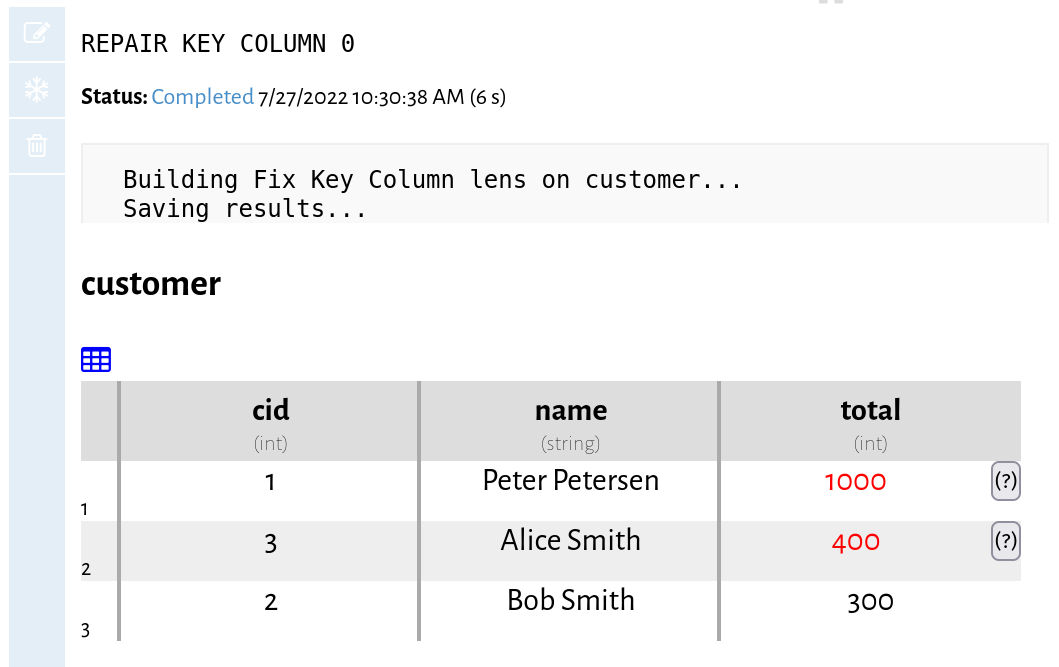
\includegraphics[width=8cm]{graphics/caveatted_data.png}
    % \begin{tabular}{c|c|c|c}
    %   \thead{cid} & \thead{name} & \thead{total} & \\       \hline
    %   1         & Peter          Petersen        & 1000 &   \\
    %   2         & Bob            Smith           & 300  & \rowcaveat  \\
    %   3         & Alice          Smith           & 400  & \rowcaveat  \\
    % \end{tabular}
    %%%%%%%%%%%%%%%%%%%%%%%%%%%%%%%%%%%%%%%%
  \caption{A UB-DB in Vizier encoding $D_1$ with possibly uncertain cells marked with caveats.}\label{fig:ub-db-encoding-d-2-with-p}
\end{wrapfigure}
%%%%%%%%%%%%%%%%%%%%%%%%%%%%%%%%%%%%%%%%
While such heuristics may be quite effective on average and are certainly superior to just randomly selecting a world, it is unavoidable that they fail for some cleaning scenarios. 
An alternative approach called consistent query answering~\cite{B11} takes a conservative stance, instead of selecting one repair, we reason about all possible repairs and only return query answers (the so-called \textit{certain answers}) that are in the query's results for every repair (i.e., are guaranteed to be in the result independent of which repair is correct). 
This approach has the advantage that only correct query answers are returned, but is computationally expensive, may exclude many very likely answers (if they are not 100\% certain), and is not closed (it is not possible to evaluate queries with certain answer semantics over the certain answers of a query).


%%%%%%%%%%%%%%%%%%%%%%%%%%%%%%%%%%%%%%%%%%%%%%%%%%%%%%%%%%%%%%%%%%%%%%%%%%%%%%%%
\subsection{Attribute- and Row-level Caveats and\\ Uncertainty-Annotated Databases}
\label{sec:attribute-row-level}
%
\begin{wrapfigure}[6]{r}[0pt]{8cm}
  \vspace*{-5mm}
  \centering
  \vspace*{-14mm}
  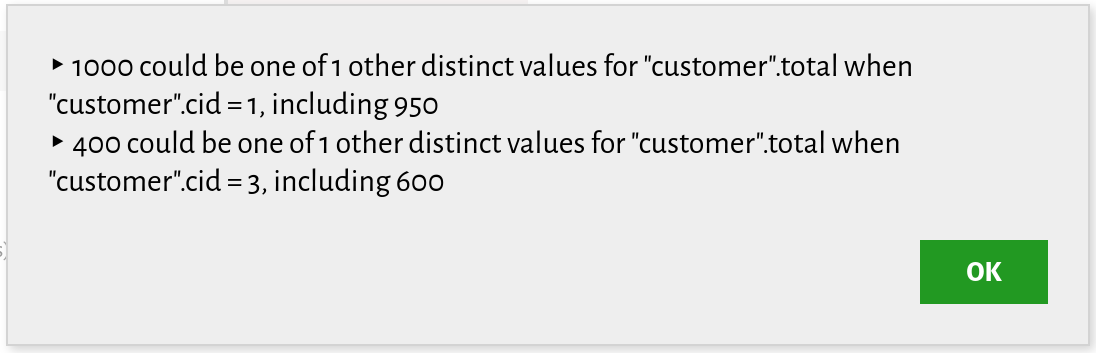
\includegraphics[width=8cm]{graphics/caveats.png}
  \caption{Caveats annotating the relation $D_1$}
\end{wrapfigure}
%


For Vizier, we developed an uncertain data model called
uncertainty-annotated databases~\cite{FH19} that annotates one
possible world (the so-called \textit{selected-guess world}) with an under-approximation  of certain answers (if we claim that a row is certain, then it is certain) that can be computed efficiently. This is encoded by annotating a subset of a dataset's rows with row-level caveats to mark them as not being certain.  The reason that we use an under-approximation is to be able to evaluate complex queries (full relational algebra including aggregation) efficiently (with PTIME data complexity and small overhead over deterministic query processing). Furthermore, attribute-level caveats are used to mark attribute values as uncertain (they may not be the same in every possible world) which is similar in nature to certain answers with nulls~\cite{L16a}.

% %%%%%%%%%%%%%%%%%%%%%%%%%%%%%%%%%%%%%%%%
% \begin{figure}[t]
%   \centering

% \begin{minipage}[b]{0.31\linewidth}
% \centering
%     \textbf{UA-DB with Selected Guess $D_1$}\\[3mm]
%     %%%%%%%%%%%%%%%%%%%%%%%%%%%%%%%%%%%%%%%
%     \begin{tabular}{c|c|c|c}
%       \thead{cid} & \thead{name} & \thead{total} & \\       \hline
%       1         & Peter          Petersen        & 1000 & \rowcaveat  \\
%       2         & Bob            Smith           & 300  & \rowcaveat  \\
%       3         & Alice          Smith           & 400  & \rowcaveat  \\
%     \end{tabular}
%     %%%%%%%%%%%%%%%%%%%%%%%%%%%%%%%%%%%%%%%%
%   \end{minipage}

%   \caption{UB-DB encoding $D_2$ with possibly uncertain rows marked with caveats (aster ix).}\label{fig:ub-db-encoding-d-2-with-p}
% \end{figure}
% %%%%%%%%%%%%%%%%%%%%%%%%%%%%%%%%%%%%%%%%

%%%%%%%%%%%%%%%%%%%%%%%%%%%%%%%%%%%%%%%%%%%%%%%%%%%%%%%%%%%%%%%%%%%%%%%%%%%%%%%%
% \subsection{Queries over Uncertainty-Annotated Databases}
% \label{sec:uncert-annot-datab}

% In~\cite{FH19} we introduced a query semantics for UA-DBs that

% %%%%%%%%%%%%%%%%%%%%%%%%%%%%%%%%%%%%%%%%%%%%%%%%%%%%%%%%%%%%%%%%%%%%%%%%%%%%%%%%
% \subsection{Implementation in Spark}
% \label{sec:implementation-spark}





%%% Local Variables:
%%% mode: latex
%%% TeX-master: "../2022_IEEE_DEB_Vizier"
%%% End:


%%%%%%%%%%%%%%%%%%%%%%%%%%%%%%%%%%%%%%%%%%%%%%%%%%%%%%%%%%%%%%%%%%%%%%%%%%%%%%%%
\section{Conclusions and Future Work}
\label{sec:conclusions}

In this paper, we have made the case for a multi-modal data science platform built on top of an incremental, data-centric workflow engine and have introduced the reader to Vizier, our system implementing this vision. 
Because each modality (notebooks, spreadsheets, the caveat view, etc\ldots) is a ``view'' interacting with the same underlying workflow and datasets, it is easy to extend the system to support new interaction paradigms in the future.  Building our system so that cells execute in isolation and only interact through dataflow makes it easy to add new cell types to the system, because we only have to worry about the interaction of the new cell type with  data artifacts. 
Thus, adding support for other interaction modalities (e.g., new programming languages) into the system is straight-forward: we implement a new cell type and an API to access Vizier artifacts from within the modality.

As demonstrated in recent preliminary work, having a scheduler that revises its schedule based on dependencies discovered at runtime and using static dataflow analysis, we can execute notebook cells in parallel and avoid re-executing cells that are guaranteed not to change during automatic refresh.
Significantly more opportunities for avoiding work exist, in particular by leveraging Vizier's standardized representation of artifacts.
For example, by representing updates to dataset artifacts as change sets, existing approaches for incremental view maintenance can reduce the runtime overhead of recomputing workflow steps, as well as the space costs of preserving multiple artifact versions. Another interesting direction for future work is to study incremental maintenance of workflow results when the definition of a workflow step changes. This is an novel variation of the traditional incremental view maintenance problem where we have to update the result based on a change to the query rather than based on a change to the data.

Similarly, standard representations of artifacts can be used to help users better understand the outputs of their workflows.
For example, numerous efforts have explored causal explanations in database query results (\cite{DBLP:conf/sigmod/KanagalLD11,DBLP:journals/pvldb/MeliouGMS11,DBLP:journals/pvldb/MeliouRS14,DBLP:journals/ftdb/GlavicMR21}, and explainability in machine learning has recently become an area of active research.
For such techniques to be truly valuable, they need to operate across artifact types. For example, what would it take to link a sudden change in predictions made by a model to the addition of a new category in source data five transformations removed from the model training step. With Vizier's uncertainty model and provenance tracking we lay the ground work to develop methods for generating explanations that span multiple steps in a workflow. 

Finally, we note that Vizier provides a ``ground-up'' approach to stitching different interaction modalities into a single workflow.
Tools implemented as views over Vizier's workflow model seamlessly interact with each other, with coarse-grained provenance, reactive cell execution, and repeatability/reproducibility.
However, these capabilities are limited to a single Vizier instance, and are of limited value to already existing tools.
An important open challenge is the design of a federated infrastructure for data analytics workflows, allowing multiple Vizier instances or unrelated tools to interoperate.


%%%%%%%%%%%%%%%%%%%%%%%%%%%%%%%%%%%%%%%%%%%%%%%%%%%%%%%%%%%%%%%%%%%%%%%%%%%%%%%%
% ACKNOWLEDGEMENTS
\mypara{Acknowledgements} This work was supported by NSF Awards ACI-1640864, IIS-1750460, IIS-1956149, and IIS-2125516. % and \ldots

%%%%%%%%%%%%%%%%%%%%%%%%%%%%%%%%%%%%%%%%%%%%%%%%%%%%%%%%%%%%%%%%%%%%%%%%%%%%%%%%
% BIBLIOGRAPHY
%\bibliographystyle{abbrv}
%\bibliography{2022_IEEE_DEB_Vizier.bib}

\documentclass[11pt]{article}

\usepackage{deauthor,times,graphicx}
\usepackage{color,colortbl}
% \usepackage[dvipsnames]{xcolor}
% \usepackage{hyperref}
\usepackage{amsmath}
\usepackage{amssymb}
\let\proof\relax
\let\endproof\relax
\usepackage{amsthm}
\usepackage{cleveref}
\usepackage{wrapfig}
\usepackage{url}
\usepackage{stmaryrd,amssymb}
\usepackage{listings}
\usepackage{algorithm}
% \usepackage[noend]{algorithmic}
\usepackage{fancybox}


%%%%%%%%%%%%%%%%%%%%%%%%%%%%%%%%%%%%%%%%
% Theorems, Definitions, Examples
%%%%%%%%%%%%%%%%%%%%%%%%%%%%%%%%%%%%%%%%
\newtheorem{theo}{Theorem}
\numberwithin{theo}{section}
\newtheorem{lem}[theo]{Lemma}
\newtheorem{propo}[theo]{Proposition}
\newtheorem{coll}[theo]{Corollary}
\newtheorem{exam}{Example}
\numberwithin{exam}{section}
\newtheorem{defi}{Definition}
\numberwithin{defi}{section}


%%%%%%%%%%%%%%%%%%%%%%%%%%%%%%%%%%%%%%%%%%%%%%%%%%%%%%%%%%%%%%%%%%%%%%%%%%%%%%%%
\usepackage{todonotes}
\newcommand{\BG}[1]{\todo[inline]{\textbf{Boris:} #1}}
\newcommand{\OK}[1]{\todo[inline]{\textbf{Oliver:} #1}}
\newcommand{\JF}[1]{\todo[inline]{\textbf{Juliana:} #1}}
\newcommand{\MB}[1]{\todo[inline]{\textbf{Mike:} #1}}

\newcommand{\jfedit}[1]{\textcolor{red} {#1}}


%%%%%%%%%%%%%%%%%%%%%%%%%%%%%%%%%%%%%%%%%%%%%%%%%%%%%%%%%%%%%%%%%%%%%%%%%%%%%%%%
% OUR SETUP
\newcommand{\mypara}[1]{\medskip\noindent\textbf{{#1}.}}

\ifdefined\thead
\else
  \newcommand{\thead}[1]{\textbf{#1}}
\fi
\newcommand{\rowcaveat}{\textbf{\textcolor{red}{$\ast$}}}
\newcommand{\pdb}{\mathcal{D}}

%%%%%%%%%%%%%%%%%%%%%%%%%%%%%%%%%%%%%%%%%%%%%%%%%%%%%%%%%%%%%%%%%%%%%%%%%%%%%%%%
% DOCUMENT
\begin{document}

%%%%%%%%%%%%%%%%%%%%%%%%%%%%%%%%%%%%%%%%%%%%%%%%%%%%%%%%%%%%%%%%%%%%%%%%%%%%%%%%
% LST DEFS

%%%%%%%%%%%%%%%%%%%%%%%%%%%%%%%%%%%%%%%%
% Colors
%%%%%%%%%%%%%%%%%%%%%%%%%%%%%%%%%%%%%%%%
\definecolor{lstpurple}{rgb}{0.5,0,0.5}
\definecolor{lstred}{rgb}{1,0,0}
\definecolor{lstreddark}{rgb}{0.7,0,0}
\definecolor{lstredl}{rgb}{0.64,0.08,0.08}
\definecolor{lstmildblue}{rgb}{0.66,0.72,0.78}
\definecolor{lstblue}{rgb}{0,0,1}
\definecolor{lstmildgreen}{rgb}{0.42,0.53,0.39}
\definecolor{lstgreen}{rgb}{0,0.5,0}
\definecolor{lstorangedark}{rgb}{0.6,0.3,0}
\definecolor{lstorange}{rgb}{0.75,0.52,0.005}
\definecolor{lstorangelight}{rgb}{0.89,0.81,0.67}
\definecolor{lstbeige}{rgb}{0.90,0.86,0.45}


% Declare bold typewriter font with Computer Modern
\DeclareFontShape{OT1}{cmtt}{bx}{n}{<5><6><7><8><9><10><10.95><12><14.4><17.28><20.74><24.88>cmttb10}{}

%%%%%%%%%% SQL + proveannce listing settings
\lstdefinestyle{psql}
{
tabsize=2,
basicstyle=\small\upshape\ttfamily,
language=SQL,
morekeywords={PROVENANCE,BASERELATION,INFLUENCE,COPY,ON,TRANSPROV,TRANSSQL,TRANSXML,CONTRIBUTION,COMPLETE,TRANSITIVE,NONTRANSITIVE,EXPLAIN,SQLTEXT,GRAPH,IS,ANNOT,THIS,XSLT,MAPPROV,cxpath,OF,TRANSACTION,SERIALIZABLE,COMMITTED,INSERT,INTO,WITH,SCN,UPDATED,PARTITION,BY,PRECEDING,FOLLOWING,CURRENT,ROW,ROWS,RANGE,GROUPING,SETS,CUBE,ROLL,UP},
extendedchars=false,
keywordstyle=\bfseries,
mathescape=true,
escapechar=@,
sensitive=true
}


%%%%%%%%%% SQL + proveannce listing settings - colorful version
\lstdefinestyle{psqlcolor}
{
tabsize=2,
basicstyle=\small\upshape\ttfamily,
language=SQL,
morekeywords={PROVENANCE,BASERELATION,INFLUENCE,COPY,ON,TRANSPROV,TRANSSQL,TRANSXML,CONTRIBUTION,COMPLETE,TRANSITIVE,NONTRANSITIVE,EXPLAIN,SQLTEXT,GRAPH,IS,ANNOT,THIS,XSLT,MAPPROV,OF,TRANSACTION,SERIALIZABLE,COMMITTED,INSERT,INTO,WITH,SCN,UPDATED},
extendedchars=false,
keywordstyle=\bfseries\color{lstpurple},
deletekeywords={count,min,max,avg,sum},
keywords=[2]{count,min,max,avg,sum,first,last,lead,lag,cxpath},
keywordstyle=[2]\color{lstblue},
stringstyle=\color{lstreddark},
commentstyle=\color{lstgreen},
mathescape=true,
escapechar=@,
sensitive=true
}


%%%%%%%%%% DATALOG style
\lstdefinestyle{datalog}
{
basicstyle=\footnotesize\upshape\ttfamily,
language=prolog
}




%%%%%%%%%% listings settings for pseudo code
\lstdefinestyle{pseudocode}
{
  tabsize=3,
  basicstyle=\small,
  language=c,
  morekeywords={if,else,foreach,case,return,in,or},
  extendedchars=true,
  mathescape=true,
  literate={:=}{{$\gets$}}1 {<=}{{$\leq$}}1 {!=}{{$\neq$}}1 {append}{{$\listconcat$}}1 {calP}{{$\cal P$}}{2},
  keywordstyle=\color{lstpurple},
  escapechar=&,
  numbers=left,
  numberstyle=\color{lstgreen}\small\bfseries,
  stepnumber=1,
  numbersep=5pt,
}

% \definecolor{pynotebookcellbg}{RGB}{247,247,247}
\definecolor{pynotebookcellbg}{gray}{0.95}

\lstdefinestyle{pynotebook}
{
  tabsize=3,
  basicstyle=\small\upshape\ttfamily,
  language=python,
  extendedchars=true,
  mathescape=true,
  morekeywords={show,read_csv,read_geojson,groupby,spatial_join,geocode,count},
  keywordstyle=\color{Blue},
  stringstyle=\itshape\color{Sepia},
  identifierstyle=\bfseries\color{OliveGreen},
  escapechar=&,
  numbers=left,
  numberstyle=\tiny\bfseries\ttfamily\color[gray]{0.7},
  stepnumber=1,
  numbersep=5pt,
  frame=single,
  frameround=tttt,
  backgroundcolor=\color{pynotebookcellbg}
}

\lstset{style=psqlcolor}

%%%%%%%%%%%%%%%%%%%%%%%%%%%%%%%%%%%%%%%%%%%%%%%%%%%%%%%%%%%%%%%%%%%%%%%%%%%%%%%%

\newcommand{\tinysection}[1]{
  \medskip \noindent \textbf{#1}.
}

%%%%%%%%%%%%%%%%%%%%%%%%%%%%%%%%%%%%%%%%%%%%%%%%%%%%%%%%%%%%%%%%%%%%%%%%%%%%%%%%
% TITLE AND AUTHORS
\title{The Right Tool for the Job: Data-Centric Workflows in Vizier}
%\title{It's a Notebook, It's a Spreadsheet, \ldots It's Vizier!}

\author{Oliver Kennedy,$^{\star}$~~Boris Glavic,$^{\diamond}$~~Juliana Freire,$^{\dagger}$~~and~~Michael Brachmann$\,^{\star}$\\
$^{\star}$~University at Buffalo, USA\\
$^{\diamond}$~Illinois Institute of Technology, USA\\
$^{\dagger}$~New York University, USA
}

\maketitle

\graphicspath{{submissions/workflow-vizier-glavic/}}

%%%%%%%%%%%%%%%%%%%%%%%%%%%%%%%%%%%%%%%%%%%%%%%%%%%%%%%%%%%%%%%%%%%%%%%%%%%%%%%%
% ABSTRACT
\begin{abstract}
  Data scientists use a wide variety of systems with a wide variety of
  user interfaces such as spreadsheets and notebooks for their data
  exploration, discovery, preprocessing, and analysis
  tasks. % For instance, spreadsheet interfaces are used for manual curation and simple types of analysis; notebook interfaces are used for data preprocessing, analysis, and visualization; and big data platforms, workflow systems, and database systems are used for more advanced querying and for deploying data analysis pipelines that were prototyped using notebooks.
  While this wide selection of tools offers data scientists the
  freedom to pick the right tool for each task, each of these tools
  has limitations (e.g., the lack of
  reproducibility % and automatic refresh of outdated results in
  of
  notebooks), % or the limited support of spreadsheets to specify batch data transformations),
  data needs to be translated between tool-specific formats, and
  common functionality such as versioning, provenance, and dealing
  with data errors often has to be implemented for each
  system. We argue that rather than alternating between task-specific
  tools, a superior approach is to build multiple user-interfaces on top
  of a single incremental workflow / dataflow platform with built-in
  support for versioning, provenance, error \& tracking, and data
  cleaning. We discuss Vizier, a notebook system that implements this
  approach, introduce the challenges that arose in building such a
  system, % , and compare the approach against state-of-the-art systems. Furthermore, we
  and highlight how our work on Vizier lead to novel research in
  uncertain data management and incremental execution of workflows.
\end{abstract}
%%%%%%%%%%%%%%%%%%%%%%%%%%%%%%%%%%%%%%%%%%%%%%%%%%%%%%%%%%%%%%%%%%%%%%%%%%%%%%%%


%%%%%%%%%%%%%%%%%%%%%%%%%%%%%%%%%%%%%%%%%%%%%%%%%%%%%%%%%%%%%%%%%%%%%%%%%%%%%%%%
\section{Introduction}
\label{sec:intro}

Federated Learning (FL) is a distributed machine learning (ML) paradigm that trains a model across a number of participating entities holding local data samples.
% , without exchanging them. 
In this work, we focus on \emph{cross-device} FL that harnesses a large number (up to hundreds of millions) of edge devices with disparate characteristics such as availability, compute, memory, or connectivity
resources~\citep{kairouz2019advances}. %that harnesses potential
% Current applications of FL are designed to scale up to client populations of hundreds of millions or even billions. 
Two challenges to the success of cross-device FL are privacy and scalability. 
FL was originally motivated for improving privacy since data points remain on client devices. 
% and only small model updates were shared to a co-ordinating server.
However, as with other forms of ML, information about training data can be extracted via membership inference or reconstruction attacks on a trained model \citep{carlini2021membership,carlini2020extracting}, or leaked through local updates~\citep{MelisSCS19,geiping2020inverting}. 
Consequently, Secure Aggregation (\SecAgg) protocols were introduced to prevent the server from directly observing individual client updates, which is a major vector for information leakage~\citep{bonavitz2019federated,huba2021papaya}. 
Additional mitigations such as  Differential Privacy (DP) may be required to offer further protection 
against attacks~\citep{dwork2006calibrating,abadi2016deep}, as discussed in Section~\ref{sec:discussion}.
% , as discussed in Section~\ref{sec:discussion}.
%As an additional layer of protection against statistical inference attacks, SecAgg is usually paired with Differential Privacy (DP) \citep{dwork2006calibrating}. To realize the full promise of FL as a privacy-enhancing technology, we need both SecAgg and Differential Privacy.

Ensuring scalability to populations of heterogeneous clients is the second challenge for FL.
% There are many aspects for FL scalability, such as ensuring that model updates can be calculated efficiently 
% by devices with various capabilities and intermittent availability~\citep{bonavitz2019federated}.
% Here, we focus on the communication bottleneck as the primary concern.
Indeed, wall-clock training times are highly correlated with increasing model and batch sizes~\citep{huba2021papaya}, even with recent efforts such as FedBuff~\citep{nguyen2021federated},
% With increasing model and batch sizes, the wall-clock training time increases accordingly~\citep{huba2021papaya}. 
% Despite efforts such as buffered asynchronous aggregation~\cite{nguyen2021federated}, 
and communication overhead between the server and clients dominates model convergence time.
% cross-device FL remains bottlenecked by communication latency between the server and the clients. 
% \karthik{should we mention this paper in a different way? Fedbuff paper doesn't explicitly call out latency as an issue, nor do we run experiments to on async fl ourselves}  \ashkan{I also think the transition can be smoother: first we focus on scalability and billions. Then we say communication is the bottleneck} 
Consequently, compression techniques were used to reduce the communication bandwidth while maintaining model accuracy.
However, a fundamental problem has been largely overlooked in the literature: in their native form, standard compression methods such as scalar quantization and pruning are not compatible with \SecAgg. 
This makes it challenging to ensure both security and communication efficiency.
% at the same time.
% the default method to provide security for client update, 
% presenting an unpleasant dichotomy between security or efficiency. 


% Second, this is the most restricted direction, since upload bandwidth remains more restricted than download. 
% In the US, fixed-line broadband speeds typically achieve a ratio of $3\times$ to $20\times$ more download bandwidth than upload
% bottlenecks remain, and so we seek to reduce the message size of clients by \textit{compression}. 
% Compression has been widely proposed in various ML scenarios, in the form of pruning (removing model parameters) and quantization (reducing fidelity of parameter representation). 
% Indeed, these techniques have been successfully used in FL settings with appreciable improvements in communication while maintaining model accuracy. 
% However, there is a fundamental problem which has been largely overlooked in the literature: in their native form, these compression methods are not compatible with SecAgg, the default method to provide security for client updates. 
% This presents an unpleasant dichotomy: we can have security or efficiency, but not both. 
%
%
% In this paper, we resolve this gap by showing how to modify FL compression techniques to make them security-friendly. We focus on compressing \emph{uplink} updates from clients to the server for two reasons. 
% First, uplink communications are subject to Secure Aggregation protocols to ensure a high security bar, while downlink updates broadcasted by the server are deemed public. 
% Second, upload bandwidth is generally more restricted than download. For instance, according to the most recent FCC report, the ratio of download to upload speeds for DSL/cable providers\footnote{Fixed-line broadband is most relevant since FL is typically restricted to using unmetered connections, usually over Wi-Fi~\citep{huba2021papaya}.} in the US ranges between 3$\times$ to 20$\times$~\citep{fcc-broadband}.
% % This requires some meticulous changes to coordinate clients to use the same global (non-private) hyperparameters, and show that this coordination does not damage model quality. 
% % For the strongest compression methods, we step outside of the SecAgg primitive and propose a new secure primitive, Secure Indexing, which enables the best compression ratios without sacrificing utility. 
% Finally, efficient and secure uplink communication brings several benefits beyond speeding up convergence: 
% lowering communication cost reduces selection bias due to undersampling clients with limited connectivity, improving fairness and inclusivity metrics. 
% It also shrinks the carbon footprint of FL, whose fraction attributable to communication can reach 95\%~\citep{qiu2021first}.
%
%In this paper, w
We address this gap by adapting compression techniques to make them compatible with \SecAgg. We focus on compressing \emph{uplink} updates from clients to the server for three reasons. 
First, uplink communication is more sensitive and so is subject to a high security bar, whereas downlink updates broadcast by the server are deemed public. 
Second, upload bandwidth is generally more restricted than download bandwidth. For instance, according to 
a recent FCC report, 
%the most recent \modif{FCC\footnote{\modif{US Federal Communications Commission.}} report}, 
the ratio of download to upload speeds for DSL and cable providers\footnote{FL is typically restricted to using unmetered connections, usually over Wi-Fi~\citep{huba2021papaya}.} in the US ranges between 3$\times$ to~20$\times$~\citep{fcc-broadband}.
% Fixed-line broadband is most relevant since
% This requires some meticulous changes to coordinate clients to use the same global (non-private) hyperparameters, and show that this coordination does not damage model quality. 
% For the strongest compression methods, we step outside of the SecAgg primitive and propose a new secure primitive, Secure Indexing, which enables the best compression ratios without sacrificing utility. 
Efficient uplink communication brings several benefits beyond speeding up convergence: 
lowering communication cost reduces selection bias due to under-sampling clients with limited connectivity, improving fairness and inclusiveness. 
It shrinks the carbon footprint of FL, the fraction of which attributable to communication can reach 95\%~\citep{qiu2021first}.
In summary, we present the following contributions: 
\begin{itemize}
    \item We highlight the fundamental mismatch between two critical components of the FL stack: \SecAgg protocols and uplink compression mechanisms.
    
    \item We formulate solutions by imposing a linearity constraint on the decompression operator, as illustrated in Figure~\ref{fig:secagg_summary} in the case of TEE-based \SecAgg.
    
    \item We adapt the popular scalar quantization and (random) pruning compression methods for compatibility with the FL stack that require no changes to the \SecAgg protocol.
    
    \item For extreme uplink compression without compromising security, we propose Secure Indexing (\SecInd), a variant of \SecAgg that supports product quantization. %and admits a secure implementation.
\end{itemize}

\begin{figure*}[t]
    \centering
    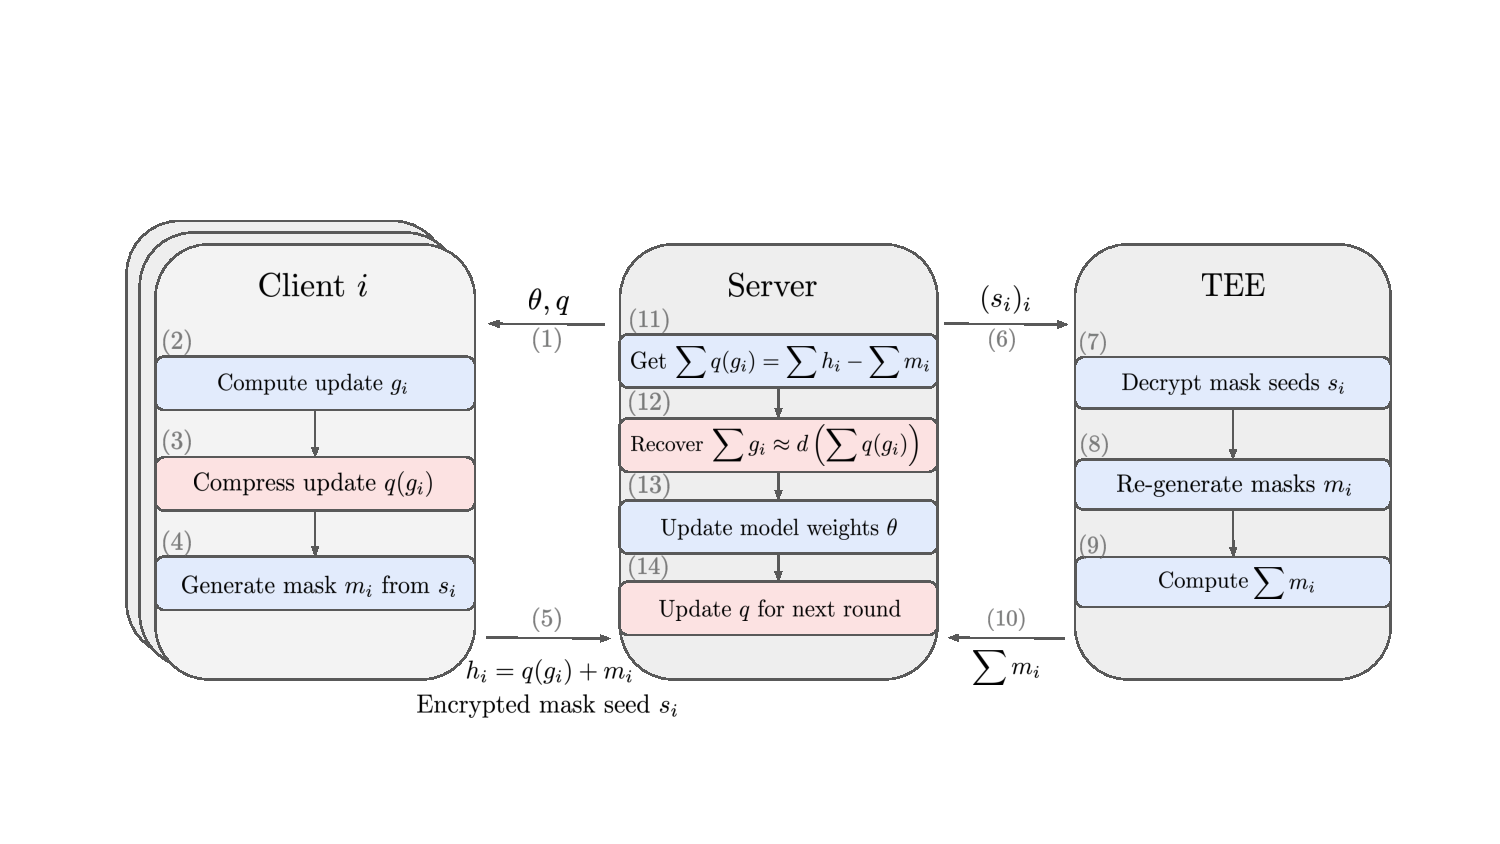
\includegraphics[width=0.8\textwidth]{figs/secagg_summary_new.pdf}
    %\vspace{-5mm}
    \caption{\label{fig:secagg_summary}
    Summary of the proposed approach for one FL round, where we omit the round dependency and \modif{Differential Privacy (DP)} for clarity. Blue boxes denote standard steps and red boxes denote additional steps for uplink compression. Client $i$ computes local model update $g_i$, compresses it with the compression operator $q$, and encrypts it by adding a random mask $m_i$ in the compressed domain, hence reducing the uplink bandwidth (steps 2--4). The server recovers the aggregate in the compressed domain by leveraging any \SecAgg protocol \modif{(steps 7--13, with a TEE-based \SecAgg, see Section~\ref{subsec:secagg})}. Since the decompression operator $d$ is linear, the server can convert the aggregate back to the non-compressed domain, up to compression error (step 12). As with the model weights $\theta$, the compression operator $q$ are also periodically updated and broadcast by the server (step 14). 
    In Section~\ref{sec:method}, we apply the proposed method to scalar quantization and pruning without impacting \SecAgg and propose Secure Indexing, a variant of \SecAgg for extreme uplink compression with product quantization. See Section~\ref{subsec:secagg} for details about \SecAgg and Section~\ref{sec:discussion} for a discussion on~DP.
    }
    \vspace{-3mm}
\end{figure*}



% Our focus in this paper is on 

%Second, scaling cross-device (synchronous) FL to millions of clients with various capabilities and intermittent availability \citep{bonavitz2019federated} suffers from diminishing returns: the wall-clock training time plateaus as the number of clients keeps increasing~\citep{huba2021papaya}. Even though this challenge can be addressed by leveraging the buffered asynchronous aggregation technique proposed by \cite{nguyen2021federated}, compatible with DP and SecAgg, the asynchronous protocol remains bottlenecked by communication latency between the server and the clients.


%Considering the above privacy and scalability goals, we focus on enabling efficient FL communications while keeping a high privacy bar. In addition to the primary objective of speeding up convergence, reducing communication costs brings other significant benefits. Lowering communication requirements addresses selection bias due to undersampling clients with limited connectivity, improving fairness and inclusivity metrics. Better communication efficiency shrinks the carbon footprint of FL, whose fraction attributable to communication can reach 95\%~\citep{qiu2021first}. %Finally, training larger model in FL would be a possibility, when the communication cost is reduced, because local memory or compute requirements can be addressed by modifying the local training loop, for instance with gradient checkpointing \citep{chen2016training}. However, some form of compression would be required to enable efficient communication.


%First, compressing model updates from the client to the server presents several challenges due to compatibility with SecAgg and is an area suitable for further research. 
%Second, upload bandwidth is generally more restricted than download. For instance, according to the most recent FCC report, the ratio of download to upload speeds for DSL/cable providers in the US ranges between 3$\times$ to 20$\times$~\citep{fcc-broadband}. We consider broadband speeds here because devices participate in the FL training while connected to fixed broadband, usually through Wi-Fi~\citep{huba2021papaya}.




% Hence, FL provides the ability to leverage data from massive client populations while ensuring the security and privacy of the client data.
% Go further: compatibility with DP / compression as a mitigation techniques of attacks
% Model and gradient compression intrinsically different.
%  Why not having the secure enclave perform the aggregation?
% \section{Requirements for a Multi-modal Data Science Platform}
\label{sec:requ-holist-data}

In this section we outline the requirements of a multi-modal data science platform and then introduce Vizier as a solution fulfilling these requirements. We start by discussing existing modalities that are widely used to interact with data in data science and their advantages and disadvantages. Converging on a set of modalities we deem to be essential, we then cover several cross-cutting concerns such as reproducibility and dealing with errors that are important no matter what modality is used to interact with data.

%%%%%%%%%%%%%%%%%%%%%%%%%%%%%%%%%%%%%%%%%%%%%%%%%%%%%%%%%%%%%%%%%%%%%%%%%%%%%%%%
\subsection{Modalities for Interacting with Data}
\label{sec:modal-inter-with}

Data scientists often employ several tools during the life-cycle of building a data pipelines. During data discovery, search engines (e.g., open data repositories) and dataset discovery tools (e.g., metadata management tools for data lakes) are used to identify data internal to an organization, data available for purchase, or openly available data that could be used to fulfill the goal the data scientist has in mind. The next step is typically to profile the data and understand its semantics and fitness for the task at hand. At this stage, data visualization is used, either in the form of specialized visualization systems or by employing visualization libraries written in, e.g., Python. This is often done from within notebook environments like Jupyter which can show visualizations inline with the users code. Afterwards, data is curated and integrated. Spreadsheets are often used for manual inspection of smaller datasets, repair of one-off errors, and to calculate basic statistics. Task-specific data cleaning systems or libraries written in a general purpose programming language are employed to (partially) automate this process. The cleaned and integrated data is then used in data analysis (e.g., building and evaluating machine learning models, running analytical queries, \ldots) and the final results of the analysis are visualized. Building a data pipeline is often an iterative process where the user revisits previous steps in the pipeline to deal with errors and to refine the processing.

%%%%%%%%%%%%%%%%%%%%%%%%%%%%%%%%%%%%%%%%%%%%%%%%%%%%%%%%%%%%%%%%%%%%%%%%%%%%%%%%
\subsubsection{Notebooks for Interactive Pipeline Development with Immediate Feedback}
\label{sec:noteb-inter-pipel}
%
Notebook systems like Jupyter and Apache Zeppelin to name just a few have become the quasi-standard for developing data science pipelines. One major advantage of notebooks is their highly interactive nature: users can run pieces of code and immediately observe their results. This makes it easy to debug steps in the pipeline and aids iterative development of pipelines. The outputs recorded in a notebook serve as a documentation of the data preparation and analysis process. Furthermore, most notebook system allow support documentation (typically written in a markup language such as markdown) to be interleaved with code. Even notebook interfaces have become prevalent, most existing implementations are suffer from poor reproducibility, do not support iterative development well, and are not suited well for large and complex pipelines. A recent study~\cite{PM19} on Jupyter notebooks collected from github observed that only 4\% of these notebooks are reproducibly in the sense that they can be rerun without errors and produce the same result as recorded in the notebook. We have argued in \cite{BS20, DG22} that these shortcomings are not inherent to the notebook model, but rather are the result of the architecture of notebook systems which use a long running kernel (e.g., a Python interpreter) and when the user runs a cell in a notebook send the cell's code to the kernel for execution. The kernels state, however, is hidden from the user and except for cell outputs is not encoded in the notebook itself. This leads to unreproducible behavior where the results recorded in the notebook no longer agree with a serial (top-down) execution of the notebook's cells. Furthermore, this can lead to stale results, if the user forgets to rerun cells whose code does dependent on the code in a cell that has been changed. Given the many benefits of and broad use of notebooks, support for a notebook interface is a must for any data science platform. We argue that by providing a notebook interface on top of a specialized workflow engine we can avoid the pitfalls of notebook systems which are thin wrappers around a kernel (Python interpreter). Specifically, we want a solution that supports a notebook interface (\textbf{requirement (N)} which fulfills the following conditions:
\begin{itemize}
\item \textbf{(N1) Serial Execution Semantics:} At any point in time, the results for the cells of the notebook agree with the results produced by a serial execution of the notebook.
\item \textbf{(N2) No Stale Outputs:} The outputs of each cell in the notebook should correctly reflect the current version of the notebook's code.
\item \textbf{(N3) Reproducibility:} The execution of a pipeline (notebook) does not depend on any hidden state. That is, as long as the code in the notebook is deterministic, rerunning a pipeline produces the same output as the original execution.
\end{itemize}

Note that any system that guarantees serial execution of notebooks as defined above, automatically guarantees that there are no stale outputs and that the execution of a notebook is reproducible.


%%%%%%%%%%%%%%%%%%%%%%%%%%%%%%%%%%%%%%%%%%%%%%%%%%%%%%%%%%%%%%%%%%%%%%%%%%%%%%%%
\subsubsection{Spreadsheets for Manual Curation and Exploration}
\label{sec:spre-manu-curat}
%
While notebooks are suited well for programmatic transformation and exploration of data, spreadsheet interfaces enable manual exploration and one-off transformations and fixes~\cite{FG16}. For instance, a user may search for and correct a few mistyped attributes values through a spreadsheet interface. Spreadsheets are also suited well for testing simple data transformations on a few rows using formulas and then once the transformation is satisfactory apply the transformation to a large number of rows by applying the same formula to many rows. Many spreadsheet systems have support for tracking changes made to the spreadsheet, but lack mechanisms to navigate the version history of a spreadsheet and to create branches, e.g., to try out a crazy idea without breaking a deployed version of a data science pipeline. As observed elsewhere~\cite{bendre-19-fhs}, spreadsheet systems do not typically scale to large datasets. While it is anyways infeasible to manually clean and curate large datasets, developing manual fixes on a sample / subset of a large dataset and then deploying the fixes to the dataset can be quite effective. Most spreadsheet systems use a data model that is incompatible with other structured data models such as the relational data model or data frames (which are essentially relations with row indexes) in that (i) columns do not have to be declared but are used by inserting a value into one cell of a column, (ii) the values of a column do not need to belong to a single datatype (e.g., some cells in a column may store strings while others are integers), and (iii) some operations  change the row and column positions rather than their content (e.g., inserting a row, changes the positions of all following rows). To support spreadsheets as a modality (\textbf{requirement (S)}, data science platforms should:
\begin{itemize}
\item \textbf{(S1) Translating between Relations and Spreadsheets:} It should be possible to manipulate standard relations through a spreadsheet view as well as process spreadsheets in other modalities.
\item \textbf{(S2) Supporting Spreadsheet Operations over Relations:} It should be possible to apply spreadsheet operations such as inserting / deleting rows / columns.
\item \textbf{(S3) Scalability:} It should be possible access large datasets through a spreadsheet interface.
\end{itemize}

%%%%%%%%%%%%%%%%%%%%%%%%%%%%%%%%%%%%%%%%%%%%%%%%%%%%%%%%%%%%%%%%%%%%%%%%%%%%%%%%
\subsubsection{Profiling and Interactive Visualizations}
\label{sec:inter-visu}
%
Data profiling and visualization are important tools for data scientists to explore data, understands its semantics, and identify problems with the data.
Data science platforms should support visualizations (\textbf{requirement (V)}). For example, a typical task in the initial data exploration phase of constructing a pipeline is to analyze and visualize the data distributions of columns in a dataset, e.g., by computing histograms for individual columns or by calculating the number of null values per column. Another common approach is to visualize correlations between columns. Both the spreadsheet and notebook modalities discussed so far, do support creation of plots and other data visualizations. Visualization recommendation~\cite{lee-21-l, hu-19-v} guide the user in exploring visualizations that help them to understand their data. A data science platform should support out-of-the-box visualizations  for common tasks (\textbf{requirement (V1)}, e.g., accessing data distributions as histograms as well as provide access to more general visualization tools (\textbf{requirement (V2)} to enable creation of custom visualization of, e.g., analysis results.

%%%%%%%%%%%%%%%%%%%%%%%%%%%%%%%%%%%%%%%%%%%%%%%%%%%%%%%%%%%%%%%%%%%%%%%%%%%%%%%%
\subsubsection{Semi-automated Data Cleaning, Curation, and Integration}
\label{sec:semi-automated-data}
%
As has been observed repeatedly in the past~\cite{nyt:wrangling}, data scientists spend the majority of their time in data discovery, preparation, and curation. Data cleaning, integration, and curation are complex tasks that are time consuming and error-prone. While full automation of these tasks is typically not an option, a plethora of semi-automated tools (e.g., constraint-based data cleaning~\cite{ilyas-15-tcrd}, schema matching~\cite{RB01}, and data integration~\cite{HR06}) which rely on heuristics and often involve the user in curation decisions have been proposed and exist in the form of stand-alone tools and libraries available for languages such as Python. Data science platforms should enable users to use such tools and algorithms in their data science pipelines (\textbf{requirement (C)}. Most approaches for automating data wrangling rely on heuristics to clean data. This is due to the fact that typically insufficient information is available to determine what the correct repair for a dataset is. For instance, when repairing a primary key constraint by tuple deletion~\cite{ilyas-15-tcrd}, one has to retain at most one tuple from each group of tuples with the same primary key value, however, we typically lack information to decide which tuple is the correct one to keep. Thus, data repair algorithms instead use heuristics such as preferring tuples with values that are common in the dataset or optimizing a global metric~\cite{RC17}. Data science platforms should track changes made based on heuristics and how they affect downstream operations as well as provide the user with an overview of what other choices did exist and how different choices would have affected the user's analysis results (\textbf{requirement (U)}):
\begin{itemize}
\item \textbf{(C) (Semi-)automated Data Curation and Integration:} Data science platforms should empower users to access (automated) data curation, cleaning, and integration techniques.
\item \textbf{(U) Tracking the Impact of Uncertain Choices:}  The impact of heuristic choices should be tracked through the operations in a data pipeline to aide the user in understanding how these choices have affected their analysis results and how the results would be affected if another alternative would have been chosen during data cleaning.
\end{itemize}

In summary, all modalities we have discussed so far have in common that they provide ways for the user to interact with data by applying transformations that create new data artifacts or update existing data artifacts and by viewing artifacts through user interfaces. For instance, plotting a histogram of the value distribution of an attribute in a csv file involves several transformations: (i) load the CSV file into a suitable in-memory data structure (e.g., a Pandas dataframe); (ii) aggregate the data to create a histogram; (iii) transform the histogram into a plot. We argue that it is feasible to build multiple modalities as ``views'' on top of a single dataflow platform. This approach has the advantage that the user does not have to to manually transform data between different formats expected by systems implementing the different modalities. Even more important, critical orthogonal functionality  such as versioning (that we will discuss next) has to only be implemented once.

%%%%%%%%%%%%%%%%%%%%%%%%%%%%%%%%%%%%%%%%%%%%%%%%%%%%%%%%%%%%%%%%%%%%%%%%%%%%%%%%
\subsection{Cross-cutting Concerns}
\label{sec:cross-cutt-conc}

Independent of which modality is used to interact with the data, there are important cross-cutting concerns such as reproducibility, supporting the user in iterative development of their data pipelines, dealing with data errors and uncertainty, and how to document data which need to be addressed. Some of the issues with implementing these cross-cutting functionality for specific modalities was already discussing in \Cref{sec:modal-inter-with}, but here we

\begin{itemize}
\item \textbf{(R) Reproducibility and Versioning:} Developing a data science pipeline typically requires several rounds of iterative development and refinement and may involve more than one developer. Keeping track of versions of the pipeline (and the associated results) in a version control manner is critical for aiding users in their development process (e.g., roll back to a past working version of the pipeline or test an experimental idea in a separate branch). However, we argue that unlike in version control systems where the user decides which versions of their code are persisted, for data science platforms it is beneficial if by default all past versions are retained (\textbf{requirement (R1)}). That is there should be no difference between the state kept for supporting undo as well as state kept for versioning. Furthermore, for reproducibility, unless the user's code contains non-deterministic operations, repeated executions of a pipeline should return the same result. Since we want to support interactive modalities like spreadsheets, modifications made through such modalities (e.g., manual edits of cell values or inserting and deleting rows in a spreadsheet) have to be translated into steps in the pipeline (\textbf{requirement (R2)}).
\item \textbf{(I) Supporting Iterative Refinement of Pipelines:} Data pipelines are typically constructed in an iterative fashion by adding additional steps and revisiting prior steps in the pipeline. For example, if an analysis returns unexpected results, the user may backtrack and modify steps in the pipeline which clean the data that is used in the analysis. A data science platform should support users in this process by (i) providing an overview of the structure of the pipeline to help the user to navigate between different parts of the pipeline (\textbf{requirement (O)}), (ii) by providing coarse-grained provenance to help the user identify which steps affected the data used by a pipeline step (\textbf{requirement (P)}), and (iii) ensure that outputs of pipeline steps are always up to date when upstream steps are modified. Note that the last requirement is the ``no stale outputs'' requirement (\textbf{requirement (N2)}) we have already discussed in \Cref{sec:noteb-inter-pipel}.
\item \textbf{(D) Documenting Data and Operations:} One advantage of notebook style interfaces is that they allow code and data to be documented using a markup language. For instance, a user may use this feature to document some insights into the semantics of their data or to explain why they selected a particular cleaning or learning technique. However, documentation in notebooks is associated with steps in the pipeline (cells in the notebook) rather than with pieces of data. While this type of documentation should be support (\textbf{requirement (D1)}), data documentation serves a wide range of purposes such as documenting data semantics (e.g., the year for a column storing dates as a month and day of the month), encoding information of how data was collected and processed, and recording information about issues with the data (e.g., a heart rate measurement is outside of the physically possible range). In \cite{kumari:2021:cidr:datasense} we argued that documentation pertaining to data is mission critical should be associated with the data (\textbf{requirement (D2)}) and should persist through operations (\textbf{requirement (D3)}). For instance, if the user annotated some values in a dataset with a note explaining that these values are suspicious, then aggregated summaries derived from the data should also be associated with these notes.
\item \textbf{(E) Dealing with Errors and Uncertainty:} Uncertainty and errors are prevalent in many application domains due to sensor, outliers~\cite{HA04}, and data entry errors, heuristics applied during data curation, integration~\cite{AS10, FK11b}, and cleaning~\cite{YM15, BS10a}, and misinterpretation of data semantics. Data science platforms should help users in identifying errors, should provide access to semi-automated (heuristic) methods for cleaning and curating data such as the data repair techniques~\cite{B19, ilyas-15-tcrd}. Furthermore, the platform should help the user to determine how choices made during cleaning (whether by a human or an algorithm) affect the results of analyzing the data.
\end{itemize}

In this section we have outlined a set of requirements, both to support specific modalities of interacting with data as well as general requirements that any system for building data science pipelines should support.


%%% Local Variables:
%%% mode: latex
%%% TeX-master: "../2022_IEEE_DEB_Vizier"
%%% End:

%!TEX root=../2022_IEEE_DEB_Vizier.tex

% %%%%%%%%%%%%%%%%%%%%%%%%%%%%%%%%%%%%%%%%
% \begin{figure}[t]
%   \centering
%   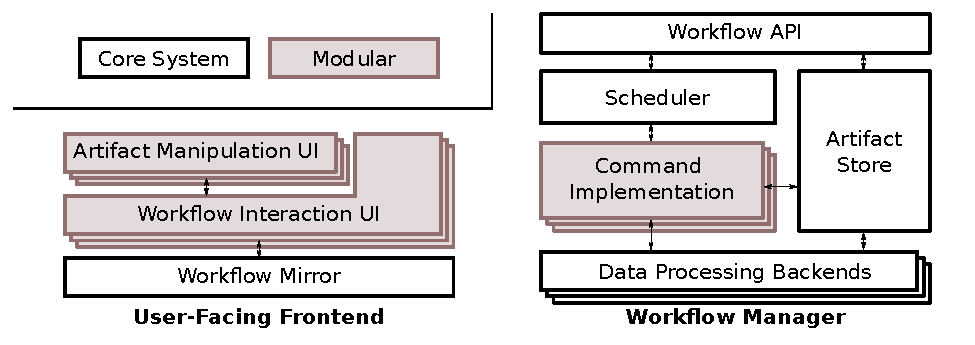
\includegraphics[width=0.7\textwidth]{graphics/systemarch}\\[-5mm]
%   \caption{Vizier's architecture, comprised of a user-facing frontend component and a backend component.}\label{fig:vizier-architecture}
% \end{figure}
% %%%%%%%%%%%%%%%%%%%%%%%%%%%%%%%%%%%%%%%%

%%%%%%%%%%%%%%%%%%%%%%%%%%%%%%%%%%%%%%%%%%%%%%%%%%%%%%%%%%%%%%%%%%%%%%%%%%%%%%%%
\pagebreak[4]
\subsection{Solution Overview}
\label{sec:solution-overview}

%%%%%%%%%%%%%%%%%%%%%%%%%%%%%%%%%%%%%%%%
\begin{wrapfigure}[12]{r}[0pt]{12cm}
  \centering
  \includegraphics[width=0.7\textwidth]{graphics/systemarch}\\[-5mm]
  \caption{Vizier's architecture, comprised of a user-facing frontend component and a backend component.}\label{fig:vizier-architecture}
\end{wrapfigure}
%%%%%%%%%%%%%%%%%%%%%%%%%%%%%%%%%%%%%%%%
An overview of Vizier's architecture is shown in \Cref{fig:vizier-architecture}.
Addressing requirement \textbf{W1}, the central abstraction in Vizier is a workflow: a linear sequence of steps. % taken by the user in pursuit of a specific objective.
Unlike classical workflow systems, Vizier does not require users to explicitly declare information flow between steps.
Rather Vizier borrows the model employed in popular computational notebooks like Jupyter, where inter-cell communication occurs through a global state (artifacts) passed sequentially through steps.
Following notebook conventions, we refer to these steps as \emph{cells}, and the global state as a \emph{scope}, a map from artifact name to the version of the artifact valid at this point in the workflow. Vizier stores artifacts in common formats through a versioned \textbf{Artifact Store} (\Cref{sec:data-artifacts}), addressing requirement \textbf{A2}.
In \Cref{sec:vizier-workflows}, we formalize Vizier's workflow model, and show how we satisfy requirement \textbf{W3} by instrumenting how each cell interacts with the scope, allowing us to determine what artifact versions are valid.

Vizier's workflow semantics, paired with the versioned artifact store and workflow versioning (\Cref{sec:vizier-history}) addresses requirement \textbf{W2}. % as notebooks have a natural concept of logical order (the order of cells in the notebook) that can be adjusted over time.
% Adding workflow versioning  is sufficient to fully address the requirement.
In contrast, classical notebooks like Jupyter or Zeppelin rely on the global state of an interpreter for inter-cell communication.
Reverting this state to an earlier revision is challenging~\cite{zelnicki:2017:nodebook}, limiting their ability to satisfy requirement \textbf{W3}.
Vizier instead relies on its versioning system, allowing its \textbf{Scheduler} to automatically detect and re-evaluate stale cells (\Cref{sec:vizier-scheduler}).
To address requirement \textbf{A3}, we designed a light-weight uncertain data model that is implemented in Vizier in the form of \textit{caveats}, annotations on data that indicate uncertain values and rows  (\Cref{sec:data-docum-error}).

Addressing requirement \textbf{A1} requires modularity in both Vizier's front- and back-end components.
First, the user's interactions with a workflow and artifacts, whether through a scripting language, graphical interaction, or any other modality, need to be captured for replay (simultaneously addressing requirement \textbf{A4}). In Vizier this is achieved by requiring that every update to an artifact made through a particular modality has to be reflected as an operation in the workflow, i.e., a data update is translated into a workflow update.
Vizier manages a collection of \textbf{Command Implementations} that implement the logic behind these artifact transformations (\Cref{sec:multimodality}).
To streamline the implementation of commands, Vizier's data formats and transformations are built over standard \textbf{Data Processing Backends} like Apache Spark.
% For example, Vizier supports fine-grained provenance over datasets by encoding them as Spark data frames.

The frontend is implemented over a \textbf{Workflow Mirror} that uses websockets to reflect a live view of the workflow the user is editing.
Vizier automatically derives a default \textbf{Artifact Manipulation User Interface} for its notebook interface from each command's parameter schemas. This interface suffices for many templated commands, but the frontend can be further extended to provide a more customized experience, for example for Spreadsheet-style direct manipulation of data (\Cref{sec:spreadsheets}).
As illustrated in \Cref{fig:screenshot}, the frontend displays three \textbf{Workflow Interaction User Interfaces} by default: (i) A direct display of the workflow as a notebook, (ii) a table of contents summary of the notebook, including highlighting from documentation, and (iii) a list of artifacts derived by the notebook.
Several of these components, including the notebook and the artifact list provide access to direct manipulation interfaces.
Additional views currently implemented in Vizier include: (iv) A caveat view (\Cref{sec:data-docum-error}) that shows and tracks potential errors in the workflow and data, (v) a history view that shows the evolution of the workflow over time, and (vi) a data provenance subway diagram view.

%%%%%%%%%%%%%%%%%%%%%%%%%%%%%%%%%%%%%%%%%%%%%%%%%%%%%%%%%%%%%%%%%%%%%%%%%%%%%%%%
\begin{figure}
  \includegraphics[width=\textwidth]{graphics/screenshot.pdf} 
  \caption{The Vizier User Interface}
  \label{fig:screenshot}
\end{figure}
%%%%%%%%%%%%%%%%%%%%%%%%%%%%%%%%%%%%%%%%%%%%%%%%%%%%%%%%%%%%%%%%%%%%%%%%%%%%%%%%

%%% Local Variables:
%%% mode: latex
%%% TeX-master: "../2022_IEEE_DEB_Vizier"
%%% End:

%!TEX root=../2022_IEEE_DEB_Vizier.tex
%%%%%%%%%%%%%%%%%%%%%%%%%%%%%%%%%%%%%%%%%%%%%%%%%%%%%%%%%%%%%%%%%%%%%%%%%%%%%%%%
\section{Versioned Data Artifact Store}
\label{sec:data-artifacts}

Steps in Vizier workflows create, read, and update \textit{``data artifacts''} or artifacts for short.
To maximize interoperability between cells, Vizier establishes standards for how these artifacts are serialized, which we now discuss. Versions of artifacts are immutable. 
An update to an artifact creates a new object representing the updated artifact. Immutability greatly simplifies handling of state in Vizier and enables us to share artifact versions across multiple revisions of a workflow.

\mypara{Dataset Artifacts}
Tabular data is represented by Vizier as a Spark dataframe~\cite{AX15}, a logical encoding of how a dataset is derived from source data.
The choice to store datasets through a logical representation (specifying the computation instead of its result) is driven largely by the need for managing annotations (requirement \textbf{A3} which is implemented by rewriting the computation to handle annotations), but also results in lower space consumption.
% Because data frames are not serializable, Vizier instead stores dataframe constructors: standardized logic for instantiating a data frame, e.g. by transforming or applying other artifacts.

% Vizier's dataframe constructors are a close analog of SparkML's \texttt{Pipeline}s, which provide a serializable representation of data frame transformation logic.
% Although Vizier provides a pipeline data frame constructor, Pipelines are strictly a representation of transformations, normally requiring glue code to apply the pipeline to an independently loaded dataset;
% Constructors completely capture the logic needed to instantiate a dataframe.

\mypara{Parameter Artifacts}
A parameter artifact can be any primitive value of any data type supported by Apache Spark; We note that this includes simple nested collections like Arrays and Maps.
This type of artifact provides a way to parameterize scripts and other system components, particularly for non-technical users.
% Vizier provides a ``Set Parameter'' command that allows users to specify parameters;
and parameter artifacts are used to pass simple data (e.g., simple constants in Python) between cells.

In addition to these two artifact types, Vizier also supports plots (stored in the vegalite~ \cite{DBLP:journals/tvcg/SatyanarayanMWH17} format), blobs and uninterpreted files, and language-specific constructs, e.g., Python function definitions. For lack of space, we do not further  discuss these other artifact types.

% \mypara{Chart Artifacts}
% Although Vizier provides means for plot generation (e.g., Bokeh, Matplotlib) through messages emitted by a cell, a standardized vegalite~\cite{DBLP:journals/tvcg/SatyanarayanMWH17} artifact format allows multiple cells to collaboratively edit a plot.
% For example, a ``Chart'' command makes it easy for users to quickly visualize a dataset, and then a Spark or Python cell can refine the resulting visualization by tweaking labels, adding markers, or adjusting colors.

% \mypara{Blob and File Artifacts}
% As a fallback to other data formats, Vizier allows cells to export state through a simple blob format.
% For example, Python falls back to encoding global state in `pickle' format, which is stored as a simple blob.
% The blob store is encoded as an in-memory array; If the artifact is large enough to warrant disk IO (e.g., a large model), requires a directory structure (e.g., parquet files), or is otherwise tied to the filesystem, Vizier provide a file artifact format.
% File artifacts are stored in a unique location tied to the artifact identifier.

% \mypara{Function Artifacts}
% Symbols representing language-specific constructs like functions, classes, and imported modules are encoded as raw code.
% Each artifact stores condains code that defines a single symbol under a specific name.
% At time of writing, support for function artifacts requires explicit cross-platform implementation support, although efforts are under way to provide a standardized cross-language interface.




%%% Local Variables:
%%% mode: latex
%%% TeX-master: "../2022_IEEE_DEB_Vizier"
%%% End:

% %!TEX root=../2022_IEEE_DEB_Vizier.tex
\section{Microkernel Notebooks}
As we outline above, a typical computational notebook relies on a kernel, a long-lived interpreter for a scripting language for a scripting language like python that retains the notebook's intermediate state.
When a cell is executed by the user, its contents are evaluated by the long running interpreter; the interpreter's state changes, and any output produced by the cell (e.g., console logs, charts, or maps) is displayed alongside the cell.
This behavior is independent of the order in which the cell appears in the notebook: The user may return to an earlier cell and modify it, but this cell is simply run against the current state of the interpreter.

Although this design allows users to revise cells in the notebook without being forced to re-run all of the notebooks code from scratch, it does pose several problems.
Most notably that it forces users to reason about the internal state of the kernel, for example by manually adopting a single static assignment variable allocation pattern.
Second, it also requires users to manually keep track of how different notebook cells relate to one-another; When a cell is modified, other cells that depend on it may also need revision.
Finally, in this design, persistence (e.g., of the results of a slow-running computation) must be managed entirely by the user.
Moreover, it is up to the user to manually manage this state to ensure consistent versioning, and portability.

One class of systems including Vizier~\cite{BS20,BB19} and Nodebook address these challenges by checkpointing global notebook state in between cell executions and restoring it when a cell is re-executed.
Thus, the cell is always evaluated on the state version emitted by the preceding cell, and changes to the state can be identified so that subsequent cells that depend on modified outputs can be re-evaluated.
This model 


\begin{itemize}
	\item Standard API for interacting with notebook state facilitates multi-modality
	\begin{itemize}
		\item No $N^2$ problem like for jupyter kernels
		\item Not just notebooks
	\end{itemize}
	\item Typed API allows fine-grained provenance
	\begin{itemize}
		\item Reproducibility
		\item Automatic refresh
		\item No hidden (mystical) dependencies
	\end{itemize}
	\item Challenges:
	\begin{itemize}
		\item Communicating state between kernels
		\item 2-dimensional version model (cell-order vs historical-order <- better name for this exists)
		\item Input/output changes in history vs Operation changes in history
		\begin{itemize}
			\item Vizier: Module vs Cell vs Result
			\item The Vizier execution state-model
		\end{itemize}
		\item Scheduling / Deciding state
	\end{itemize}
\end{itemize}

%%% Local Variables:
%%% mode: latex
%%% TeX-master: "../2022_IEEE_DEB_Vizier"
%%% End:

%!TEX root=../2022_IEEE_DEB_Vizier.tex
\section{Workflow Provenance Model and Runtime}
\label{sec:vizier-workflows}

In this section, we outline Vizier's workflow and versioning model, how we determine which cells of a workflow need to be re-executed if a cell is changed, and introduce the parallel scheduler of the system.

% multi-tiered, two-dimensional provenance model.
% We first relate the model to both classical workflow provenance and modern computational notebooks, then discuss how Vizier's model incorporates a temporal dimension, and finally discuss state invalidation and re-evaluation.

\newcommand{\notebook}{\mathcal N}
\newcommand{\workflow}{\mathcal W}
\newcommand{\artifact}{a}
\newcommand{\nbcell}{c}
\newcommand{\outputval}{o}
\newcommand{\readset}{\vec r}
\newcommand{\writeset}{\vec w}
\newcommand{\globalscope}{\mathcal G}
\newcommand{\outputdomain}{\mathcal O}
\newcommand{\valuedomain}{\mathcal D}
\newcommand{\undefinedval}{\bot}
\newcommand{\unknownval}{\circledcirc}
\newcommand{\keyset}{\texttt{keys}}
\newcommand{\changeset}{\Delta}
\newcommand{\variabledomain}{\Sigma}
\newcommand{\diff}[2]{\Delta(#1, #2)}
\newcommand{\evalnb}[1]{\llbracket #1 \rrbracket}

\begin{figure}
  \centering
  \begin{minipage}{0.9\textwidth}
  \begin{lstlisting}[style=pynotebook]
data = read_csv("social_data.csv")
show(data)
  \end{lstlisting}

  \begin{lstlisting}[style=pynotebook]
data["latlon"] = geocode(data["address"])
show(data)
  \end{lstlisting}

  \begin{lstlisting}[style=pynotebook]
censusblocks = read_geojson("blocks.json")
show(censusblocks)
  \end{lstlisting}

  \begin{lstlisting}[style=pynotebook]
data = spatial_join(data, censusblocks, ["latlon", "geometry"])
count_per_block = data.groupby("block_id").count()
show(count_per_block)
  \end{lstlisting}
  \end{minipage}\\[-4mm]
  \caption{A simplified example notebook}
  \label{fig:exampleNotebook}
\end{figure}

%%%%%%%%%%%%%%%%%%%%%%%%%%%%%%%%%%%%%%%%%%%%%%%%%%%%%%%%%%%%%%%%%%%%%%%%%%%%
%%%%%%%%%%%%%%%%%%%%%%%%%%%%%%%%%%%%%%%%%%%%%%%%%%%%%%%%%%%%%%%%%%%%%%%%%%%%
\subsection{Workflow Model}
\label{sec:vizier:eval}

A workflow in Vizier is a sequence of workflow steps (cells) that can read and write artifacts. 
Artifacts are versioned at the granularity of cells. 
A cell writing an artifact $\artifact$ causes a new version of $\artifact$ to be created. 
We will discuss the APIs Vizier exposes to the data interaction modalities for accessing artifacts in \Cref{sec:multimodality}. 
The semantics of a Vizier workflow is the serial execution of the cells of the workflow, where the latest version of each artifact is passed as input to the cell that will be executed next. 
Thus, as long as the cells themselves are deterministic, the artifact versions created by the execution of a workflow are uniquely determined by the workflow itself.

%%%%%%%%%%%%%%%%%%%%%%%%%%%%%%%%%%%%%%%%%%%%%%%%%%%%%%%%%%%%%%%%%%%%%%%%%%%%%%%%
\begin{exam}
  \label{ex:introduction}
  \Cref{fig:exampleNotebook} shows a notebook with a simplified data ingestion, cleaning, and analysis task.
  The notebook loads the dataset (cell 1), geocodes listed street addresses (cell 2), loads a collection of census blocks (cell 3), and computes summary statistics for each census block (cell 4).
  We use this  notebook to illustrate a key challenge of traditional  notebook architectures.
  %
  The user modifies cell 2 to switch to a different geocoder, potentially requiring re-evaluation of the notebook.
  In this specific notebook, the user had the foresight to write in an idempotent style, making it unnecessary to re-run cell 1 to recover the state needed to run cell 2 correctly.
  It is also unnecessary to re-run cell 3, as it does not depend on the output of cell 2.
  However, in traditional notebooks like Jupyter the burden of deciding which cells to re-evaluate rests on the user, creating added overhead and increasing the chance of errors.
\end{exam}
%%%%%%%%%%%%%%%%%%%%%%%%%%%%%%%%%%%%%%%%%%%%%%%%%%%%%%%%%%%%%%%%%%%%%%%%%%%%%%%%

Formally, a Vizier workflow is a sequence $\notebook = \{ \nbcell_1, \ldots, \nbcell_N \}$ of cells. 
The versions of artifacts valid after execution of cell $\nbcell_i$ are modeled as a global scope $\globalscope$ that maps artifact names to artifact versions or the distinguished symbol $\undefinedval$, which indicates that no version of the artifact has been produced yet.  
A cell $\nbcell$ is a function that takes a scope $\globalscope$ as input and produces an updated scope $\globalscope'$: $\nbcell (\globalscope) = \globalscope'$. 
We use $\readset_{\globalscope,i}$ to denote the names of artifacts accessed by cell $\nbcell_i$ applied to $\globalscope_i$. 
The scope parameter is necessary, because a cell may dynamically decide which artifacts to read based on the content of other artifacts.
%
The result $\evalnb{\notebook}$ of  evaluating workflow $\notebook = \{ \nbcell_1, \ldots, \nbcell_N \}$ is defined as the scope $\globalscope_n$ produced by starting with an empty scope $\globalscope_0$ (where all artifact names are mapped to $\undefinedval$), and by computing $\globalscope_{i} = \nbcell_{i}(\globalscope_{i-1})$.








% Cell evaluation in Vizier happens in notebook-order.

% Each cell is (conceptually) evaluated on the scope emitted by the preceding cell.
% Like the workflow systems that inspired it, Vizier retains inter-cell snapshots of scope to preserve notebook-order evaluation semantics while still allowing users to backtrack.


% Denote by $\globalscope$ a global scope that we will formalize shortly;

% We model a cell $\nbcell (\globalscope) = (\globalscope', \readset, \outputval)$ as a deterministic function applied to a global scope that returns a new global scope $\globalscope'$, a read set $\readset$, and an opaque output object $\outputval$ in $\outputdomain$.
% Evaluating the notebook $\evalnb{\notebook} = (\globalscope_N, [\outputval_1, \ldots, \outputval_N)$ produces a final scope $\globalscope_N$ and a sequence of outputs $\outputval_1, \ldots, \outputval_N$ through straightforward composition, starting with an empty scope $\globalscope_0$.
% %  formalized as:
% % $$(\globalscope_i, \readset_i, \outputval_i) = \nbcell_i(\globalscope_{i-1})$$
% % In the above,

%%%%%%%%%%%%%%%%%%%%%%%%%%%%%%%%%%%%%%%%
\begin{wrapfigure}[8]{r}[0pt]{11cm}
  \centering
  \vspace{-4mm}
  \includegraphics[width=10.5cm]{graphics/eval.pdf}\\[-5mm]
  \caption{Evaluation logic for the example notebook in \Cref{fig:exampleNotebook}.  Edges are labeled with global scope versions.  Cells that are (re-)evaluated are highlighted, dotted lines represent simulated state flow.}
  \label{fig:exampleEval}
\end{wrapfigure}
%%%%%%%%%%%%%%%%%%%%%%%%%%%%%%%%%%%%%%%%
If workflow $\notebook$ is modified by replacing a cell $\nbcell_i$ with a cell $\nbcell_i'$ (denoted as $\notebook[\nbcell_i \backslash \nbcell_i']$), we need to obtain the updated scope $\evalnb{\notebook[\nbcell_i \backslash \nbcell_i']}$. Of course this can be achieved by evaluating $\notebook[\nbcell_i \backslash \nbcell_i']$.
% In lieu of naively re-evaluating the notebook from scratch,
However, to improve performance,  Vizier attempts to update the output of $\evalnb{\notebook}$ by only re-evaluating a subset of the cells.
First, observe that $\globalscope_1, \ldots, \globalscope_{i-1}$ are independent of $\nbcell_i$; and remain unchanged if $\nbcell_i$ is modified.
It is still necessary to have $\globalscope_{i-1}$ to evaluate $\nbcell_i'$; so Vizier caches all intermediate global scopes after evaluating each workflow revision.

% \begin{figure}
%   \centering
%   \includegraphics[width=0.7\textwidth]{graphics/eval.pdf}
%   \caption{Evaluation logic for the example notebook in \Cref{fig:exampleNotebook}.  Edges are labeled with global scope versions.  Cells that are (re-)evaluated are highlighted, dotted lines represent simulated state flow.}
%   \label{fig:exampleEval}
% \end{figure}

Naively, we have to still re-evaluate $\nbcell_{i+1}, \ldots, \nbcell_{N}$ using the new scope produced by $\nbcell_i'$. Let us denote the scopes produced by this evaluation as
$\globalscope_{i+1}', \ldots, \globalscope_{n}$.
% $\outputval_{i+1}', \ldots, \outputval_{N}'$.
Vizier uses the readsets $\readset_{\globalscope, i+1}, \ldots, \readset_{\globalscope, N}$, to identify cells $\nbcell_{j}$ for which the same output (artifact versions written by the cell) in $\evalnb{\notebook[\nbcell_i \backslash \nbcell_i']}$ is guaranteed. 
Denote by $\changeset(\globalscope, \globalscope') = \{ k |  \globalscope(k) \neq \globalscope'(k)\}$ the names of artifacts that differ between $\globalscope$ and $\globalscope'$. 
We have to re-execute cell $\nbcell_{i+1}$ if an artifact read by $\nbcell_{i+1}$ has changed, which is the case if $\changeset(\globalscope_i, \globalscope_i') \cap \readset_{\globalscope,i+1} \neq \emptyset$. If $\nbcell_{i+1}$ needs to be re-executed, then we set $\globalscope_{i+1}' = \nbcell_{i+1}(\globalscope_{i}')$. Otherwise, we generate $\globalscope_{i+1}$ by merging the changes made by $\nbcell_{i+1}$ in $\notebook$ to $\globalscope_{i}$ into $\globalscope_{i}'$. That is, for all artifacts $k$ we set
$\globalscope_{i+1}'(k) =   \globalscope_{i+1}(k)$ if $k \in \changeset(\globalscope_i, \globalscope_{i+1})$
and $\globalscope_{i+1}'(k) = \globalscope_{i}'(k)$ otherwise.
% begin{cases}
%   \globalscope_{i+1}(k) &\;\;\;\text{\textbf{if}}\,k \in \changeset(\globalscope_i, \globalscope_{i+1})\\
%   \globalscope_{i}'(k) &\;\;\;\text{\textbf{otherwise}}\\
% \end{cases}$$
 The same approach is applied to decide whether to evaluate or skip the remaining cells in $\notebook[\nbcell_i \backslash {\nbcell_i}']$.


% We formalize a global scope $\globalscope = \{ k_1 \rightarrow v_1, k_2 \rightarrow v_2, \ldots \}$ as a total mapping from an infinite alphabet of variable names $k \in \variabledomain$ to a set of domain values $v \in \valuedomain \cup \{\undefinedval\}$.
% The distinguished symbol $\undefinedval$ denotes an ``undefined'' value, and we assume that finitely many elements of $\variabledomain$ are mapped to non-$\undefinedval$ values (i.e., that $\globalscope$ has finite support).
% Denote by $\keyset(\globalscope) = \{ k | (k \rightarrow v) \in \writeset \wedge v \neq \undefinedval\}$ the keys of the finite support of $\globalscope$.
% Denote by $\changeset(\globalscope, \globalscope') = \{ k |  \globalscope(k) \neq \globalscope'\}$ the change set between $\globalscope$ and $\globalscope'$.

% Given the newly computed $\globalscope_i'$, we want to know if $\nbcell_{i+1}$ needs to be evaluated as well;
% If $\nbcell_{i+1}(\globalscope_i') = (\globalscope_{i+1}', \readset_{i+1}', \outputval_{i+1}')$, we can avoid re-evaluating $\nbcell_{i+1}$ if we can prove that $\outputval_{i+1} = \outputval_{i+1}'$.
% Under the assumption that $\nbcell_{i+1}$ is deterministic with respect to inputs $\readset_{i+1}$, we can guarantee that $\outputval_{i+1} = \outputval_{i+1}'$ when $\readset_{i+1} \cap \changeset(\globalscope_{i}, \globalscope_{i}')$ is empty.
% If we do not need to re-evaluate $\nbcell_{i+1}$, we can reconstruct its output by considering how the original evaluation affected the scope: the write set $\writeset_{i+1} = \changeset(\globalscope_{i}, \globalscope_{i+1})$.
% Concretely $\outputval_{i+1}' = \outputval_{i+1}$, $\readset_{i+1}' = \readset_{i+1}$ and
% $$\globalscope_{i+1}'(k) = \begin{cases}
% \globalscope_{i+1}(k) \textbf{ if } k \in \writeset_{i+1}\\
% \globalscope_{i}'(k) \textbf{ otherwise}
% \end{cases}$$
% \noindent The remaining cells of the notebook are processed in a like manner.

 %%%%%%%%%%%%%%%%%%%%%%%%%%%%%%%%%%%%%%%%%%%%%%%%%%%%%%%%%%%%%%%%%%%%%%%%%%%%%%%%
\begin{exam}
  \Cref{fig:exampleEval} continues the running example from \Cref{ex:introduction}.
  The user has replaced the initial version of cell $\nbcell_2$ with an updated version ${\nbcell_2}'$.
  The global scope produced by preceding cells ($\globalscope_1$) may be re-used unchanged to evaluate ${\nbcell_2}'$, producing scope $\globalscope_2'$.
  $\changeset(\globalscope_2, \globalscope_2')$ is the \lstinline{data} artifact, but the readset of $\nbcell_3$ is empty, and so this cell does not need to be re-evaluated.
  Instead $\globalscope_3'$ is derived by merging variables the cell previously changed (i.e., $\changeset(\globalscope_2, \globalscope_3)$) into the current global scope.
  Finally, Vizier identifies that an element of $\readset_{\globalscope,4}$ (the \lstinline{data} variable) has changed between $\globalscope_3$ and $\globalscope_3'$, necessitating a re-evaluation of cell 4.
\end{exam}
 %%%%%%%%%%%%%%%%%%%%%%%%%%%%%%%%%%%%%%%%%%%%%%%%%%%%%%%%%%%%%%%%%%%%%%%%%%%%%%%%

% \mypara{Frozen Cells}
% Vizier allows users to ``freeze'' cells, temporarily replacing them with no-op commands, but preserving all user-interface elements (including cell outputs), and allowing the cell to be easily re-inserted into the notebook.
% This allows users to quickly disable cells with transient purposes (e.g., sampling cells), or avoid triggering expensive computations while working on an earlier part of the notebook.

% \begin{figure}
%   \centering
%   \includegraphics[width=0.45\textwidth]{graphics/history.pdf}\\[-3mm]
%   \caption{History for the running example, assuming cell B was changed as in \Cref{fig:exampleEval}.}
%   \label{fig:exampleHistory}
% \end{figure}

%%%%%%%%%%%%%%%%%%%%%%%%%%%%%%%%%%%%%%%%%%%%%%%%%%%%%%%%%%%%%%%%%%%%%%%%%%%%
%%%%%%%%%%%%%%%%%%%%%%%%%%%%%%%%%%%%%%%%%%%%%%%%%%%%%%%%%%%%%%%%%%%%%%%%%%%%
\subsection{Versioning Workflows}
\label{sec:vizier-history}

%%%%%%%%%%%%%%%%%%%%%%%%%%%%%%%%%%%%%%%%
\begin{wrapfigure}[10]{r}[0pt]{8cm}
  \centering
  \includegraphics[width=0.45\textwidth]{graphics/history.pdf}\\[-3mm]
  \caption{History for the running example, assuming cell 2 was changed as in \Cref{fig:exampleEval}.}
  \label{fig:exampleHistory}
\end{wrapfigure}
%%%%%%%%%%%%%%%%%%%%%%%%%%%%%%%%%%%%%%%%
Vizier maintains a branching history of the evolution of the notebook.
% We use the term workflow ($\workflow = c_1, \ldots, c_N$) to denote a single state of the notebook.
A cell is further subdivided into (i) \textbf{cell metadata} ($c_i$) that is unique to the workflow (e.g., timestamps and execution status), (ii) \textbf{results} ($r_i$) of executing the cell, and (iii) a \textbf{module} ($m_i$) describing the command executed in the cell.
The latter two components (results and modules) may be shared across workflows.
% In other words, a single cell object acts as a many-to-many-to-many (i.e., 3-ary) relationship between workflow, module, and result entities.
A module object describes the command to be evaluated in a cell.  
This includes its type (e.g., Python or Scala script; SQL query; or one of the graphical widgets), as well as any parameters to the command (e.g., the script itself, or the artifact name to materialize query results as). 
A results object stores references to versions of artifacts in the artifact store created by the execution of the cell. 
We do not materialize the full global scope after each cell, but rather only the changes made to the global scope by the cell (i.e., the cell's write set). 
Any global scope $\globalscope_i$ can be reconstructed from the preceding write sets.

% A results object consists of three items: (i) Messages output by the cell (i.e., $\outputval$), (ii) The cell's readset as a list of name/artifact pairs, and (iii) The cell's writeset as a list of name/artifact pairs.
% Deletion is encoded by writing the distinguished value \texttt{null} to a name.
% As a performance optimization, name/artifact pairs do not embed the artifact literal, but rather a unique artifact identifier.
% This allows for efficient equivalence testing, while avoiding duplication; For example, a ``copy artifact" instruction only needs to clone the artifact identifier under a new name, and not the entire artifact.

% \mypara{Global scope}
% Note that the organizational structure used to persist history information differs from the global scope model used to reason about cell re-use.
% However, the two representations are equivalent.
% Denote by $m_1 \circ m_2$ the right-preferenced composition of \emph{partial} maps $m_1$ and $m_2$ as follows:
% $$m_1 \circ m_2 = \{ k\rightarrow v | (k \rightarrow v) \in m_1 \wedge \not\exists v' \text{ s.t. } (k \rightarrow v') \in m_2 \} \cup m_2$$
% Any global scope $\globalscope_N$ can be recovered by composing the preceding writesets: $\globalscope_N = \globalscope_0 \circ \writeset_1 \circ \ldots \circ \writeset_N$


\begin{exam}
 \Cref{fig:exampleHistory} continues our running example, which in our new terminology is a single branch comprised of two workflows $\workflow_1$ and $\workflow_2$.
  Both notebooks are comprised of four cell objects each.
  Cells 1, 3, and 4 were unchanged between workflows, and so the corresponding cell objects for $\workflow_2$ reference the same module description object as the corresponding cell for $\workflow_1$, while the module descriptions referenced by $\nbcell_2$ and ${\nbcell_2}'$ differ.
  Cells 1 and 3 do not need to be re-evaluated, and so can share their result objects, while Cells 2 and 4 both require re-evaluation and create new result objects.
\end{exam}

%%%%%%%%%%%%%%%%%%%%%%%%%%%%%%%%%%%%%%%%%%%%%%%%%%%%%%%%%%%%%%%%%%%%%%%%%%%%%%%%
\mypara{Workflow and Branch History}
Similar to version control systems like git, each workflow version in Vizier stores a reference to the workflow version it was derived from.
% The difference between workflow versions can be computed by comparing the sequence of modules referenced by the workflow's cells; but simple summary information including the type of change (insert, delete, update) and the affected module (if appropriate) is cached with the workflow object.
A branch is an append-only sequence of workflow versions. % with associated metadata (e.g., a branch name).
The branch contains a reference to the most recent workflow version in the branch. % prior versions are tracked through the series of derived-from references in the workflows themselves.
A new branch may be created from any existing workflow version, including a historical one.

%%%%%%%%%%%%%%%%%%%%%%%%%%%%%%%%%%%%%%%%%%%%%%%%%%%%%%%%%%%%%%%%%%%%%%%%%%%%
%%%%%%%%%%%%%%%%%%%%%%%%%%%%%%%%%%%%%%%%%%%%%%%%%%%%%%%%%%%%%%%%%%%%%%%%%%%%
\subsection{Parallel Scheduler}\label{sec:vizier-scheduler}

The evaluation model presented in \Cref{sec:vizier:eval} relies exclusively on \textit{dynamic provenance}, where Vizier is informed about the readset and writeset of a cell at runtime when the cell accesses artifacts through Vizier's API.
% that assist in determining whether a cell needs to be re-evaluated.
However, dynamic provenance is not always sufficient.
For example, Vizier evaluates cells in parallel where possible, but dynamic provenance is not available until the cell has already been evaluated.
Static provenance, which can derive a cell's read and write sets through static dataflow analysis of its source code, can be computed upfront.
However, static dataflow analysis is of necessity an approximation for some cell types; language features like control flow and dynamic code evaluation can lead to over- (or under-) estimates of the cell's read and write sets. % , especially with respect to a specific global scope.
Vizier uses a novel approach which refines static provenance at runtime using dynamic provenance~\cite{DG22}.

Fundamentally, Vizier's scheduler needs to assign each cell in a running workflow to one of four lifecycle stages: (i) \textbf{DONE} when the cell has a valid result object, (ii) \textbf{PENDING} when the cell depends (directly or transitively) on a cell that does not have a result object, and (iii) \textbf{RUNNING} when the cell's dependencies have a valid result object but the cell itself does not.
We further distinguish as (iv) \textbf{STALE} those cells in the \textbf{PENDING} stage for which we can conclusively determine that re-evaluation is required.
% Lifecycle stage transitions are monotonic.

To manage lifecycle transitions, Vizier's scheduler relies on a combination of static and dynamic provenance~\cite{DG22}.
It uses static provenance to generate an over-approximation on the read and write dependencies of a cell\footnote{As we argue in~\cite{DG22}, to deal with languages that support dynamic code evaluation such as Python, it would be necessary to allow under-approximations of read and write sets (missed data dependencies) and compensate for them at runtime. However, this not implemented in Vizier yet; attempts to dynamically read variables not in the maximal readset are flagged as errors.}.
  % Vizier does not presently support purely dynamic dependencies through e.g., dynamic code evaluation.  A read or write access on a variable not discovered through static analysis triggers an execution error.}.
Accordingly, the scheduler tracks an over-approximation of the read and writesets at each step of the workflow, and refines them when the execution of cell finishes and we know its precise read and write set. 
This approximation is used by Vizier's scheduler to omit cells from re-execution or schedule them for parallel execution if we can determine that it is safe to do so based on these over-approximations.

% Approximate global scopes generalize our prior definition of a global scope by extending the value domain to include the value $\unknownval$, denoting an unresolved value (i.e. variables in an approximate global scope are drawn from $\valuedomain \cup \{\undefinedval, \unknownval\}$).
% Like a regular global scope, an approximate global scope is derived by concatenating writesets ($\globalscope_i = \globalscope_{i-1} \circ \writeset_i$).
% However, if the cell is in a lifecycle stage other than \textbf{DONE}, its previous writeset is not valid.
% Instead, Vizier uses static analysis to derive an upper bound on the writeset $\writeset_{\max} \subseteq \variabledomain$, the maximal set of variables that the cell is allowed to write to.
% When the cell's writeset is not (or may not be) valid, the approximate global scope is instead updated by making each element of $\writeset_{\max}$ an unknown:
% $\globalscope_{i} = \globalscope_{i-1} \circ \{ k \rightarrow \unknownval | k \in \writeset_{\max, i} \}$

% \Cref{alg:lifecycleStage} explains how Vizier derives the lifecycle stage of a cell from the global scope emitted by the preceding cell, the cell's readset (if it exists), and the bound on the readset derived from static analysis.
% The first consideration is whether the cell's prior result object is still valid.
% If there is no prior result object (e.g., because the cell is newly inserted), or if the prior result object is definitely invalid (i.e., because a previously read value was definitely overwritten by a re-evaluated cell), the cell must be re-evaluated.
% What remains is whether the cell can be immediately evaluated (all variables in the upper bound on the readset are defined), or not.

% \begin{algorithm}
% \caption{\lstinline{lifecycle_stage}($\globalscope$, $\readset$, $\readset_{\max}$)}
% \label{alg:lifecycleStage}
% \begin{algorithmic}
%   \REQUIRE{$\globalscope$: The approximate global scope from the prior cell.}
%   \REQUIRE{$\readset$: Either a partial map from $\variabledomain$ to $\valuedomain$ denoting the actual read set if one exists, or $\unknownval$ if the cell is new.}
%   \REQUIRE{$\readset_{\max}$: A set over $\variabledomain$, denoting the statically derived upper bound on the cell's read set.}
%   \ENSURE{$\ell$: The current lifecycle stage of the cell.}
%   \IF{$\readset = \unknownval$ or there exists a $(k \rightarrow v) \in \readset$ such that $\globalscope(k) \neq \unknownval$ and $\globalscope(k) \neq v$}
%     \IF{there exists a $k \in \readset_{\max}$ such that $\globalscope(k) = \unknownval$}
%       \STATE $\ell = \textbf{STALE}$
%         \COMMENT{The cell needs to be re-evaluated, but is missing a dependency}
%     \ELSE
%       \STATE $\ell = \textbf{RUNNING}$
%         \COMMENT{The cell needs to be re-evaluated, and is ready to run}

%     \ENDIF
%   \ELSIF{there exists a $(k \rightarrow v) \in \readset$ where $\globalscope(k) = \unknownval$}
%     \STATE $\ell = \textbf{PENDING}$
%       \COMMENT{The cell may not need re-evaluation, but we don't know yet.}
%   \ELSE
%     \STATE $\ell = \textbf{DONE}$
%       \COMMENT{We can guarantee that the cell does not need re-evaluation.}
%   \ENDIF
% \end{algorithmic}
% \end{algorithm}

% When a cell transitions into the \textbf{RUNNING} state, the scheduler starts the corresponding cell.
% When the cell finishes, it has a state that matches the preceding global state, and transitions into the \textbf{DONE} state.

%%% Local Variables:
%%% mode: latex
%%% TeX-master: "../2022_IEEE_DEB_Vizier"
%%% End:
% %!TEX root=../2022_IEEE_DEB_Vizier.tex
\section{Microkernel Notebooks}
As we outline above, a typical computational notebook relies on a kernel, a long-lived interpreter for a scripting language for a scripting language like python that retains the notebook's intermediate state.
When a cell is executed by the user, its contents are evaluated by the long running interpreter; the interpreter's state changes, and any output produced by the cell (e.g., console logs, charts, or maps) is displayed alongside the cell.
This behavior is independent of the order in which the cell appears in the notebook: The user may return to an earlier cell and modify it, but this cell is simply run against the current state of the interpreter.

Although this design allows users to revise cells in the notebook without being forced to re-run all of the notebooks code from scratch, it does pose several problems.
Most notably that it forces users to reason about the internal state of the kernel, for example by manually adopting a single static assignment variable allocation pattern.
Second, it also requires users to manually keep track of how different notebook cells relate to one-another; When a cell is modified, other cells that depend on it may also need revision.
Finally, in this design, persistence (e.g., of the results of a slow-running computation) must be managed entirely by the user.
Moreover, it is up to the user to manually manage this state to ensure consistent versioning, and portability.

One class of systems including Vizier~\cite{BS20,BB19} and Nodebook address these challenges by checkpointing global notebook state in between cell executions and restoring it when a cell is re-executed.
Thus, the cell is always evaluated on the state version emitted by the preceding cell, and changes to the state can be identified so that subsequent cells that depend on modified outputs can be re-evaluated.
This model 


\begin{itemize}
	\item Standard API for interacting with notebook state facilitates multi-modality
	\begin{itemize}
		\item No $N^2$ problem like for jupyter kernels
		\item Not just notebooks
	\end{itemize}
	\item Typed API allows fine-grained provenance
	\begin{itemize}
		\item Reproducibility
		\item Automatic refresh
		\item No hidden (mystical) dependencies
	\end{itemize}
	\item Challenges:
	\begin{itemize}
		\item Communicating state between kernels
		\item 2-dimensional version model (cell-order vs historical-order <- better name for this exists)
		\item Input/output changes in history vs Operation changes in history
		\begin{itemize}
			\item Vizier: Module vs Cell vs Result
			\item The Vizier execution state-model
		\end{itemize}
		\item Scheduling / Deciding state
	\end{itemize}
\end{itemize}

%%% Local Variables:
%%% mode: latex
%%% TeX-master: "../2022_IEEE_DEB_Vizier"
%%% End:

%!TEX root=../2022_IEEE_DEB_Vizier.tex

\section{Multimodality}
\label{sec:multimodality}

As noted in \Cref{sec:vizier-history}, cells in Vizier implement a variety of different modalities, including scripting languages (e.g., Python, Scala), query languages (e.g., SQL), as well as graphical widgets for data ingestion, transformation, and curation (e.g., Load Dataset, Pivot Table, Repair Key).
We refer to the evaluation logic for each modality as \emph{cell command}.
Each cell in a Vizier workflow identifies the command that should run to evaluate the cell, along with a set of arguments to that command.
For example, the SQL cell (\texttt{sql.query}) takes two arguments: the text of a SQL query, and an optional name to materialize the result table as. In this section, we discuss how these modalities are implemented as cell types in Vizier. % and how they are presented in Vizier's notebook view.

A command is defined by the following methods:
(i) \textbf{schema}: Returns a schema for the arguments the command accepts;
(ii) \textbf{summary(arguments)}: Returns a textual description of the behavior of the command when parameterized by the provided arguments;
(iii) \textbf{dependencies(arguments)}: Returns the over-approximation of the set of names of artifacts read (resp., written) by the cell as parameterized by the provided arguments, or indicates that either or both bounds can not be computed; and
(iv) \textbf{evaluate(arguments, context)}: Evaluates the cell on the command, parameterized by the provided arguments and a context object.

The context object on which commands are evaluated provides a read/write interface to the global scope and a way to emit messages to be displayed alongside the cell in the notebook view.
As we discuss in \Cref{sec:vizier-workflows}, the global scope maps artifact names to artifact versions.
Artifacts are not persisted directly as part of the global scope, but rather are references to our write-only artifact store.\footnote{As mentioned before, artifact versions are immutable in Vizier which simplifies version management. We leave optimizations that selectively violate this policy and update artifacts or store deltas instead of creating full updated versions of artifacts to future work.}
When a cell implementation writes an artifact through the context, the artifact version is serialized and written into the artifact store.
The artifact store assigns the artifact (version) a unique identifier, which is then saved into the scope.
Similarly, to read an artifact, a cell implementation first reads the artifact identifier out of the scope, and then accesses the corresponding artifact version from the store.


%\subsection{Language APIs}
% \mypara{Language APIs}
Cells implementing runtimes for general-purpose languages need to provide users of those languages with a way to interact with the global notebook state.
This entails (i) providing a mechanism to reference the scope and import artifacts within a language-specific format, and (ii) predicting how the user-provided code will interact with the state to bound provenance.

\mypara{Python}
%
Python cells are evaluated in an independent interpreter to avoid concurrency bottlenecks from the global interpreter lock (GIL).
Thus, a key challenge is minimizing the volume of state transferred into and out of each interpreter.
Global scope is lazily loaded by populating the global state with a set of proxy objects, one for each artifact in the scope. % We discuss this based on the example of Python and SQL cells.
%
% When a variable is accessed, the proxy object is ``hydrated'' from the artifact store; From that point on, the proxy object routes all function invocations, property accesses, and operator overload invocations to the hydrated artifact.
% Several small values, including primitive constants and module references, are not compatible with proxy objects, but are small enough to allow them to be hydrated in all cells with negiligible performance cost.
%
Access to the Vizier context for messaging and artifact access occurs through a control bus that, by default, operates over the python process' standard input and output streams.
% Python's normal standard output and error streams are overridden and any output over these channels is converted into control messages; Standard input is disabled for the user-provided script.
Vizier defines a special `show' command within the module to produce structured messages (analogous to placing an item on the last line of a Jupyter cell).
The show command includes support for most Vizier-defined types, matplotlib and bokeh plots, and provides fallbacks using the Jupyter-standard \texttt{\_repr\_html\_} method, or direct stringification as a final resort.
% Vizier also discourages direct file IO by overriding the \texttt{open} command to print a warning message.
%
For predictive dependency tracking, and to identify variables that are modified, Vizier relies on Python's \texttt{ast} module, which provides an introspective compilation and code analysis framework.
Vizier performs lightweight dependency analysis~\cite{DG22} to bound the cell's read and write dependencies.

% identify variables accessed or modified by the cell's code.
% This analysis is used both to bound the read and write dependencies, as well as to determine which variables are exported into the global scope at the end of the cell.
% The AST module is also used to extract code for exported function, module, and class symbols.

\mypara{SQL}
%
SQL cells are parsed and evaluated by Apache Spark.
% Spark provides a convenient global catalog, allowing access to named functions, tables, and other values.
% However, because the specific assignment of names to values varies depending on position in the notebook, relying on the global catalog is not thread-safe.
% Instead,
Vizier intercepts the parsed SQL query AST and manually injects references to the corresponding artifacts --- either datasets or python functions --- where needed.
Spark-provided view name decorators make it possible for the injected views to retain their names from the query, avoiding incomprehensible error messages.
The same injection logic is also used to statically identify exact read and write dependencies.

% Spark has native support for Python User-Defined Functions, but this support is geared towards users accessing spark through its python frontend (\texttt{pyspark}).
% Crucially, it relies on a customized serialization format (\texttt{cloud-pickle}) that is not portable across versions of the serialization library or python.
% When Vizier identifies a reference to a python-defined UDF in a SQL query, it spins up a python interpreter, serializes the UDF, and caches it for subsequent use.

% \mypara{Scala}
% Scala cells are run directly within the Vizier JVM through the Scala reflection toolbox.
% % This feature of Scala allows scala code to be compiled and evaluated at runtime; including support for access to global state.
% % The evaluated code does not have access to local variables; Vizier works around this by passing state in through a thread-local global variable.
% % Like Python cells, Vizier overrides the \texttt{print} and \texttt{println} methods to produce messages rather than standard out.
% At present, access to global state in a scala cell occurs manually; A \texttt{vizierdb} object is created to allow cells to interact with the global scope, or to display more elaborate messages than text allows.
% Similarly, at time of writing, dependency analysis is not yet supported.


%%% Local Variables:
%%% mode: latex
%%% TeX-master: "../2022_IEEE_DEB_Vizier"
%%% End:

% 
\section{The Notebook Modality}\label{sec:notebook-modality}



%%% Local Variables:
%%% mode: latex
%%% TeX-master: "../2022_IEEE_DEB_Vizier"
%%% End:

%!TEX root=../2022_IEEE_DEB_Vizier.tex
\section{Interactive Spreadsheets}
\label{sec:spreadsheets}

A key feature of Vizier is support for direct interaction with artifacts~\cite{BS20}, most notably a spreadsheet-like interface for interacting with Spark Data Frames.
Spreadsheets provide a data exploration experience that is distinct from notebooks.
Users are limited to a single dataset, but have significantly more flexibility when exploring the data.
For example, it is common on small datasets (e.g., under 1000 rows) for users to complete preliminary data cleaning tasks like outlier detection, data integration, repair of typos and outliers, and even some limited computation (e.g., deriving new fields) in a spreadsheet prior to working with the data further (e.g., in a notebook).
Another common use case is manual data entry; The user may enter the entire dataset, or may generate a data entry template (e.g., with a script) and import the resulting file into another tool.

% In both cases, the relationship to the original dataset, and any consequent provenance information is lost.
Vizier's spreadsheet interface is intended to provide a view over a subset of the notebook, allowing users to interact with the dataset in the appropriate modality, while simultaneously preserving workflow provenance  through interactions.
% Furthermore, our goal is to present the spreadsheet as a View over a subset of the notebook.
As the user interacts with the spreadsheet, their edits are reflected in the notebook as new cells.
As the user edits the notebook, their edits are likewise reflected in the spreadsheet --- If the source data frame is updated in the notebook, Vizier attempts to re-apply the user's edits to the updated data.

\mypara{Track Changes as a View}
%
To support bi-directional interaction between spreadsheet and notebook views, Vizier implements a series of specialized cell types that mimic SQL DDL and DML operations, allowing for inserting, deleting, or reordering columns and rows, or for updating individual cell values.
We refer to the operations described by these cell types collectively as the Vizual language~\cite{FG16,BS20}.

Vizual is based on the principle that the user's interactions with a database  can be modeled as views over an original version of the data.
As prior work has shown, a view defined over a table can mimic the effects of any DDL~\cite{DBLP:journals/pvldb/CurinoMZ08} or DML~\cite{DBLP:journals/pvldb/NiuALFZGKLG17} operation applied to the table.
Analogously, each Vizual cell in the notebook uses Spark's standard data frame manipulation language to apply a successive transformation to the dataset that mimics the user's interaction.
To ensure that the spreadsheet remains responsive, a shim layer tentatively injects predicted updates to the user's interactions until the effects of the user's edit are fully applied~(e.g., as \cite{DBLP:conf/icde/GuptaDGUW09}).

In SQL DML, update operations specify target rows by a predicate.
By contrast, operations in a spreadsheet explicitly target specific rows of data, requiring Vizier to assign unique identifiers to each record to encode their order in the spreadsheet\footnote{We assume that the number of columns will remain manageable and reference them purely by name}.
To allow Vizual operations to be replayed as source data changes, these identifiers should remain stable through data transformations.
For derived data, Vizier uses a row identity model similar to GProM's~\cite{DBLP:journals/debu/ArabFGLNZ17} encoding of provenance.
Derived rows, such as those produced by declaratively specified table updates, are identified by an appropriate combination of input tuple identifiers. For example, rows in the output of a join are identified by combining identifiers from the source rows that produced them into a single identifier, and rows in the output of a projection or selection use the identifier of the source row that produced them.
% as follows:
% (i) Rows in the output of a projection or selection use the identifier of the source row that produced them;
% (ii) Rows in the output of a \texttt{UNION ALL} are identified by merging the identifier of the source row with an identifier marking which side of the union the row came from (note that this change renders the \texttt{UNION} operator non-commutative).
% (iii) Rows in the output of a cross product or join are identified by combining identifiers from the source rows that produced them into a single identifier; and (iv) Rows in the output of an aggregate are identified by each row's group-by attribute values.

The remaining challenge is assigning row identifiers to source data, which we want to remain stable through changes to the source data so that spreadsheet operations can be replayed.
Ideally, the data would include a unique identifier that we can leverage; but this is not always the case.
Storing the data in a revision control system~\cite{DBLP:conf/cidr/BhardwajBCDEMP15,DBLP:journals/pvldb/HuangXLEP17}, is not always a viable option~\cite{DBLP:conf/sigmod/AlagiannisBBIA12}.
A more heavyweight approach is to link records across revisions of a dataset~\cite{DBLP:conf/sigmod/YilmazWXNEP18}, but this adds non-negligible overhead to common-case data revisions.
Vizier presently supports persistent identifiers through append- or edit-only revisions by assigning each record a unique identifier based on its position, and a hash of its contents.
This approach has the benefit of being lightweight (it can be applied in a single pass), and resilient.
In contrast to simply using a hash-based identifier, the approach supports duplicate records.
Conversely, solely using a position-based identifier could lead to spreadsheet operations being applied to the wrong row in case of insertions.
%
While techniques for creating identifiers that are stable under updates has been studied extensively for XML databases (e.g., ORDPATH~\cite{DBLP:conf/sigmod/ONeilOPCSW04}) and recently also for spreadsheet views of relational databases~\cite{DBLP:journals/pvldb/BendreSZZCP15}, the main challenge we face in Vizier is how to retain row identity when a new version of a dataset is loaded into Vizier, as opposed to keeping identity consistent once the data is already in the system.
% In this scenario we only have access to two (identifier-free) snapshots of the dataset and no further information on how they relate to each other.

%% Local Variables:
%%% mode: latex
%%% TeX-master: "../2022_IEEE_DEB_Vizier"
%%% End:

%!TEX root=../2022_IEEE_DEB_Vizier.tex

%%%%%%%%%%%%%%%%%%%%%%%%%%%%%%%%%%%%%%%%%%%%%%%%%%%%%%%%%%%%%%%%%%%%%%%%%%%%%%%%
\section{Data Documentation, Error, and Uncertainty Management with Caveats}
\label{sec:data-docum-error}

Like notebook systems, Vizier enables users to document their workflow through markdown cells which do not manipulate artifacts, but simply serve as documentation. 
However, some documentation is specific to individual artifacts, or their component parts (e.g., rows, or columns); 
We would like such documentation to accompany the data as it is transformed~\cite{kumari:2021:cidr:datasense}.
Like other annotation management systems including Mondrian~\cite{GK05} and DBNotes~\cite{bhagwat-05-anmsrd},
Vizier empowers users to annotate data with textual comments. 
However, in contrast to these systems, in Vizier these annotations also have a precise semantics: they encode uncertainty about an attribute value of a row or the existence of a row. 
This is important, because uncertainty arises naturally in most data science pipelines (e.g., because of errors in the data or because of heuristic choices during data cleaning) and if data analysis ignores the uncertainty in the data, it can lead to analysis results that cannot be trusted.
To address this issue, caveats are propagated through operations on dataset artifacts in Vizier using an efficient uncertain query semantics we have developed~\cite{FH19, FH21}. 
Thus, caveats on values and rows in the result of an analysis conducted using Vizier encode information about how data cleaning and curation operations on the data used in the analysis affect the analysis result. 
Furthermore, Vizier's implementation of data cleaning operations introduce caveats to encode information about other possible repairs.

%%%%%%%%%%%%%%%%%%%%%%%%%%%%%%%%%%%%%%%%%%%%%%%%%%%%%%%%%%%%%%%%%%%%%%%%%%%%%%%%
\subsection{Incomplete Databases}
\label{sec:incomplete-databases}

Formally, caveats in Vizier are based on an approximation of incomplete databases. An incomplete database $\pdb = \{D_1, \ldots, D_n\}$ is a set of deterministic databases called possible worlds that encode alternative possibilities for the state of the real world: one possible world corresponds to the actual state of the real world, but we do not know which. 
As an example, consider an analyst that has to find the names of important customers (e.g., who ordered products totaling more than \$500). 
An example instance is shown in \Cref{fig:example-customer-database}. 
A common method for primary key repair is to group rows by their PK values and select one row from each group to be retained. 
However, typically we have insufficient information to know which row is the correct choice and will have to rely on heuristics (e.g., selecting the most recently updated row if this information is available). 
Incomplete databases can be used to model this uncertainty: we create an incomplete database whose worlds are all the repairs of the database violating the constraint~\cite{DBLP:journals/vldb/BeskalesIGG14}.
\Cref{fig:example-customer-database} shows two (out of 4) possible repairs for this dataset.

%%%%%%%%%%%%%%%%%%%%%%%%%%%%%%%%%%%%%%%%
\begin{figure}[t]
  \centering

  \begin{minipage}[b]{0.31\linewidth}
\centering
    \textbf{Customer Relation}\\[3mm]
    %%%%%%%%%%%%%%%%%%%%%%%%%%%%%%%%%%%%%%%%
    \begin{tabular}{c|c|c}
      \thead{cid} & \thead{name} & \thead{total} \\     \hline
      1         & Peter          Petersen        & 1000 \\
      1         & Peter          Petersen        & 950  \\
      2         & Bob            Smith           & 300  \\
      3         & Alice          Smith           & 400  \\
      3         & Alice          Smith           & 600  \\
    \end{tabular}
    %%%%%%%%%%%%%%%%%%%%%%%%%%%%%%%%%%%%%%%%
  \end{minipage}
%
  \begin{minipage}[b]{0.31\linewidth}
\centering
    \textbf{Possible       World           (Repair) $D_1$}\\[3mm]
    %%%%%%%%%%%%%%%%%%%%%%%%%%%%%%%%%%%%%%%
    \begin{tabular}{c|c|c}
      \thead{cid} & \thead{name} & \thead{total} \\       \hline
      1         & Peter          Petersen        & 1000   \\
      2         & Bob            Smith           & 300    \\
      3         & Alice          Smith           & 400    \\
    \end{tabular}
    %%%%%%%%%%%%%%%%%%%%%%%%%%%%%%%%%%%%%%%%
  \end{minipage}
%
  \begin{minipage}[b]{0.31\linewidth}
\centering
    \textbf{Possible       World           (Repqir) $D_2$}\\[3mm]
    %%%%%%%%%%%%%%%%%%%%%%%%%%%%%%%%%%%%%%%
    \begin{tabular}{c|c|c}
      \thead{cid}   & \thead{name} & \thead{total} \\       \hline
      1           & Peter          Petersen        & 1000   \\
      2           & Bob            Smith           & 300    \\
      3           & Alice          Smith           & 600    \\
    \end{tabular}
    %%%%%%%%%%%%%%%%%%%%%%%%%%%%%%%%%%%%%%%%
  \end{minipage}


  %%%%%%%%%%%%%%%%%%%%%%%%%%%%%%%%%%%%%%%%
  \begin{minipage}{0.31 \textwidth}
    \centering
    \textbf{Certain Answers}\\[3mm]
    %%%%%%%%%%%%%%%%%%%%%%%%%%%%%%%%%%%%%%%%
    \begin{tabular}{c}
      \thead{name}\\ \hline
      Peter Petersen \\
    \end{tabular}
    %%%%%%%%%%%%%%%%%%%%%%%%%%%%%%%%%%%%%%%%
  \end{minipage}
  %%%%%%%%%%%%%%%%%%%%%%%%%%%%%%%%%%%%%%%%
  %
  %%%%%%%%%%%%%%%%%%%%%%%%%%%%%%%%%%%%%%%%
  \begin{minipage}{0.31 \textwidth}
    \centering
    \textbf{Answers in $D_1$}\\[3mm]
    %%%%%%%%%%%%%%%%%%%%%%%%%%%%%%%%%%%%%%%%
    \begin{tabular}{c}
      \thead{name}\\ \hline
      Peter Petersen \\
    \end{tabular}
    %%%%%%%%%%%%%%%%%%%%%%%%%%%%%%%%%%%%%%%%
  \end{minipage}
  %%%%%%%%%%%%%%%%%%%%%%%%%%%%%%%%%%%%%%%%
  %
  %%%%%%%%%%%%%%%%%%%%%%%%%%%%%%%%%%%%%%%%
  \begin{minipage}{0.31 \textwidth}
    \centering
    \textbf{Answers in $D_2$}\\[3mm]
    %%%%%%%%%%%%%%%%%%%%%%%%%%%%%%%%%%%%%%%%
    \begin{tabular}{c}
      \thead{name}\\ \hline
      Peter Petersen \\
      Alice Smith\\
    \end{tabular}
    %%%%%%%%%%%%%%%%%%%%%%%%%%%%%%%%%%%%%%%%
  \end{minipage}
  %%%%%%%%%%%%%%%%%%%%%%%%%%%%%%%%%%%%%%%%


  \caption{Example customer database violating the primary key constraint that cid is unique and two possible worlds corresponding to some of the possible repairs of the database achieved by selecting one row among each group of rows with the same primary key value.}\label{fig:example-customer-database}
\end{figure}
%%%%%%%%%%%%%%%%%%%%%%%%%%%%%%%%%%%%%%%%

Typical constraint-repair algorithms will select one repair (one possible world) based on a heuristic like selecting the row whose values are most common in the dataset~\cite{RC17}. For instance, the cleaning algorithm may choose $D_1$ and the user would then evaluate their query (shown below) over $D_1$.

\begin{lstlisting}
                  SELECT name FROM Customer WHERE total > 500;
\end{lstlisting}

%%%%%%%%%%%%%%%%%%%%%%%%%%%%%%%%%%%%%%%%
\begin{wrapfigure}[15]{r}[0pt]{8cm}
  \centering
    % \textbf{UA-DB with Selected Guess $D_1$}\\[3mm]
    %%%%%%%%%%%%%%%%%%%%%%%%%%%%%%%%%%%%%%%
    \includegraphics[width=8cm]{graphics/caveatted_data.png}
    % \begin{tabular}{c|c|c|c}
    %   \thead{cid} & \thead{name} & \thead{total} & \\       \hline
    %   1         & Peter          Petersen        & 1000 &   \\
    %   2         & Bob            Smith           & 300  & \rowcaveat  \\
    %   3         & Alice          Smith           & 400  & \rowcaveat  \\
    % \end{tabular}
    %%%%%%%%%%%%%%%%%%%%%%%%%%%%%%%%%%%%%%%%
  \caption{A UB-DB in Vizier encoding $D_1$ with possibly uncertain cells marked with caveats.}\label{fig:ub-db-encoding-d-2-with-p}
\end{wrapfigure}
%%%%%%%%%%%%%%%%%%%%%%%%%%%%%%%%%%%%%%%%
While such heuristics may be quite effective on average and are certainly superior to just randomly selecting a world, it is unavoidable that they fail for some cleaning scenarios. 
An alternative approach called consistent query answering~\cite{B11} takes a conservative stance, instead of selecting one repair, we reason about all possible repairs and only return query answers (the so-called \textit{certain answers}) that are in the query's results for every repair (i.e., are guaranteed to be in the result independent of which repair is correct). 
This approach has the advantage that only correct query answers are returned, but is computationally expensive, may exclude many very likely answers (if they are not 100\% certain), and is not closed (it is not possible to evaluate queries with certain answer semantics over the certain answers of a query).


%%%%%%%%%%%%%%%%%%%%%%%%%%%%%%%%%%%%%%%%%%%%%%%%%%%%%%%%%%%%%%%%%%%%%%%%%%%%%%%%
\subsection{Attribute- and Row-level Caveats and\\ Uncertainty-Annotated Databases}
\label{sec:attribute-row-level}
%
\begin{wrapfigure}[6]{r}[0pt]{8cm}
  \vspace*{-5mm}
  \centering
  \vspace*{-14mm}
  \includegraphics[width=8cm]{graphics/caveats.png}
  \caption{Caveats annotating the relation $D_1$}
\end{wrapfigure}
%


For Vizier, we developed an uncertain data model called
uncertainty-annotated databases~\cite{FH19} that annotates one
possible world (the so-called \textit{selected-guess world}) with an under-approximation  of certain answers (if we claim that a row is certain, then it is certain) that can be computed efficiently. This is encoded by annotating a subset of a dataset's rows with row-level caveats to mark them as not being certain.  The reason that we use an under-approximation is to be able to evaluate complex queries (full relational algebra including aggregation) efficiently (with PTIME data complexity and small overhead over deterministic query processing). Furthermore, attribute-level caveats are used to mark attribute values as uncertain (they may not be the same in every possible world) which is similar in nature to certain answers with nulls~\cite{L16a}.

% %%%%%%%%%%%%%%%%%%%%%%%%%%%%%%%%%%%%%%%%
% \begin{figure}[t]
%   \centering

% \begin{minipage}[b]{0.31\linewidth}
% \centering
%     \textbf{UA-DB with Selected Guess $D_1$}\\[3mm]
%     %%%%%%%%%%%%%%%%%%%%%%%%%%%%%%%%%%%%%%%
%     \begin{tabular}{c|c|c|c}
%       \thead{cid} & \thead{name} & \thead{total} & \\       \hline
%       1         & Peter          Petersen        & 1000 & \rowcaveat  \\
%       2         & Bob            Smith           & 300  & \rowcaveat  \\
%       3         & Alice          Smith           & 400  & \rowcaveat  \\
%     \end{tabular}
%     %%%%%%%%%%%%%%%%%%%%%%%%%%%%%%%%%%%%%%%%
%   \end{minipage}

%   \caption{UB-DB encoding $D_2$ with possibly uncertain rows marked with caveats (aster ix).}\label{fig:ub-db-encoding-d-2-with-p}
% \end{figure}
% %%%%%%%%%%%%%%%%%%%%%%%%%%%%%%%%%%%%%%%%

%%%%%%%%%%%%%%%%%%%%%%%%%%%%%%%%%%%%%%%%%%%%%%%%%%%%%%%%%%%%%%%%%%%%%%%%%%%%%%%%
% \subsection{Queries over Uncertainty-Annotated Databases}
% \label{sec:uncert-annot-datab}

% In~\cite{FH19} we introduced a query semantics for UA-DBs that

% %%%%%%%%%%%%%%%%%%%%%%%%%%%%%%%%%%%%%%%%%%%%%%%%%%%%%%%%%%%%%%%%%%%%%%%%%%%%%%%%
% \subsection{Implementation in Spark}
% \label{sec:implementation-spark}





%%% Local Variables:
%%% mode: latex
%%% TeX-master: "../2022_IEEE_DEB_Vizier"
%%% End:


%%%%%%%%%%%%%%%%%%%%%%%%%%%%%%%%%%%%%%%%%%%%%%%%%%%%%%%%%%%%%%%%%%%%%%%%%%%%%%%%
\section{Conclusions and Future Work}
\label{sec:conclusions}

In this paper, we have made the case for a multi-modal data science platform built on top of an incremental, data-centric workflow engine and have introduced the reader to Vizier, our system implementing this vision. 
Because each modality (notebooks, spreadsheets, the caveat view, etc\ldots) is a ``view'' interacting with the same underlying workflow and datasets, it is easy to extend the system to support new interaction paradigms in the future.  Building our system so that cells execute in isolation and only interact through dataflow makes it easy to add new cell types to the system, because we only have to worry about the interaction of the new cell type with  data artifacts. 
Thus, adding support for other interaction modalities (e.g., new programming languages) into the system is straight-forward: we implement a new cell type and an API to access Vizier artifacts from within the modality.

As demonstrated in recent preliminary work, having a scheduler that revises its schedule based on dependencies discovered at runtime and using static dataflow analysis, we can execute notebook cells in parallel and avoid re-executing cells that are guaranteed not to change during automatic refresh.
Significantly more opportunities for avoiding work exist, in particular by leveraging Vizier's standardized representation of artifacts.
For example, by representing updates to dataset artifacts as change sets, existing approaches for incremental view maintenance can reduce the runtime overhead of recomputing workflow steps, as well as the space costs of preserving multiple artifact versions. Another interesting direction for future work is to study incremental maintenance of workflow results when the definition of a workflow step changes. This is an novel variation of the traditional incremental view maintenance problem where we have to update the result based on a change to the query rather than based on a change to the data.

Similarly, standard representations of artifacts can be used to help users better understand the outputs of their workflows.
For example, numerous efforts have explored causal explanations in database query results (\cite{DBLP:conf/sigmod/KanagalLD11,DBLP:journals/pvldb/MeliouGMS11,DBLP:journals/pvldb/MeliouRS14,DBLP:journals/ftdb/GlavicMR21}, and explainability in machine learning has recently become an area of active research.
For such techniques to be truly valuable, they need to operate across artifact types. For example, what would it take to link a sudden change in predictions made by a model to the addition of a new category in source data five transformations removed from the model training step. With Vizier's uncertainty model and provenance tracking we lay the ground work to develop methods for generating explanations that span multiple steps in a workflow. 

Finally, we note that Vizier provides a ``ground-up'' approach to stitching different interaction modalities into a single workflow.
Tools implemented as views over Vizier's workflow model seamlessly interact with each other, with coarse-grained provenance, reactive cell execution, and repeatability/reproducibility.
However, these capabilities are limited to a single Vizier instance, and are of limited value to already existing tools.
An important open challenge is the design of a federated infrastructure for data analytics workflows, allowing multiple Vizier instances or unrelated tools to interoperate.


%%%%%%%%%%%%%%%%%%%%%%%%%%%%%%%%%%%%%%%%%%%%%%%%%%%%%%%%%%%%%%%%%%%%%%%%%%%%%%%%
% ACKNOWLEDGEMENTS
\mypara{Acknowledgements} This work was supported by NSF Awards ACI-1640864, IIS-1750460, IIS-1956149, and IIS-2125516. % and \ldots

%%%%%%%%%%%%%%%%%%%%%%%%%%%%%%%%%%%%%%%%%%%%%%%%%%%%%%%%%%%%%%%%%%%%%%%%%%%%%%%%
% BIBLIOGRAPHY
%\bibliographystyle{abbrv}
%\bibliography{2022_IEEE_DEB_Vizier.bib}

\documentclass[11pt]{article}

\usepackage{deauthor,times,graphicx}
\usepackage{color,colortbl}
% \usepackage[dvipsnames]{xcolor}
% \usepackage{hyperref}
\usepackage{amsmath}
\usepackage{amssymb}
\let\proof\relax
\let\endproof\relax
\usepackage{amsthm}
\usepackage{cleveref}
\usepackage{wrapfig}
\usepackage{url}
\usepackage{stmaryrd,amssymb}
\usepackage{listings}
\usepackage{algorithm}
% \usepackage[noend]{algorithmic}
\usepackage{fancybox}


%%%%%%%%%%%%%%%%%%%%%%%%%%%%%%%%%%%%%%%%
% Theorems, Definitions, Examples
%%%%%%%%%%%%%%%%%%%%%%%%%%%%%%%%%%%%%%%%
\newtheorem{theo}{Theorem}
\numberwithin{theo}{section}
\newtheorem{lem}[theo]{Lemma}
\newtheorem{propo}[theo]{Proposition}
\newtheorem{coll}[theo]{Corollary}
\newtheorem{exam}{Example}
\numberwithin{exam}{section}
\newtheorem{defi}{Definition}
\numberwithin{defi}{section}


%%%%%%%%%%%%%%%%%%%%%%%%%%%%%%%%%%%%%%%%%%%%%%%%%%%%%%%%%%%%%%%%%%%%%%%%%%%%%%%%
\usepackage{todonotes}
\newcommand{\BG}[1]{\todo[inline]{\textbf{Boris:} #1}}
\newcommand{\OK}[1]{\todo[inline]{\textbf{Oliver:} #1}}
\newcommand{\JF}[1]{\todo[inline]{\textbf{Juliana:} #1}}
\newcommand{\MB}[1]{\todo[inline]{\textbf{Mike:} #1}}

\newcommand{\jfedit}[1]{\textcolor{red} {#1}}


%%%%%%%%%%%%%%%%%%%%%%%%%%%%%%%%%%%%%%%%%%%%%%%%%%%%%%%%%%%%%%%%%%%%%%%%%%%%%%%%
% OUR SETUP
\newcommand{\mypara}[1]{\medskip\noindent\textbf{{#1}.}}

\ifdefined\thead
\else
  \newcommand{\thead}[1]{\textbf{#1}}
\fi
\newcommand{\rowcaveat}{\textbf{\textcolor{red}{$\ast$}}}
\newcommand{\pdb}{\mathcal{D}}

%%%%%%%%%%%%%%%%%%%%%%%%%%%%%%%%%%%%%%%%%%%%%%%%%%%%%%%%%%%%%%%%%%%%%%%%%%%%%%%%
% DOCUMENT
\begin{document}

%%%%%%%%%%%%%%%%%%%%%%%%%%%%%%%%%%%%%%%%%%%%%%%%%%%%%%%%%%%%%%%%%%%%%%%%%%%%%%%%
% LST DEFS

%%%%%%%%%%%%%%%%%%%%%%%%%%%%%%%%%%%%%%%%
% Colors
%%%%%%%%%%%%%%%%%%%%%%%%%%%%%%%%%%%%%%%%
\definecolor{lstpurple}{rgb}{0.5,0,0.5}
\definecolor{lstred}{rgb}{1,0,0}
\definecolor{lstreddark}{rgb}{0.7,0,0}
\definecolor{lstredl}{rgb}{0.64,0.08,0.08}
\definecolor{lstmildblue}{rgb}{0.66,0.72,0.78}
\definecolor{lstblue}{rgb}{0,0,1}
\definecolor{lstmildgreen}{rgb}{0.42,0.53,0.39}
\definecolor{lstgreen}{rgb}{0,0.5,0}
\definecolor{lstorangedark}{rgb}{0.6,0.3,0}
\definecolor{lstorange}{rgb}{0.75,0.52,0.005}
\definecolor{lstorangelight}{rgb}{0.89,0.81,0.67}
\definecolor{lstbeige}{rgb}{0.90,0.86,0.45}


% Declare bold typewriter font with Computer Modern
\DeclareFontShape{OT1}{cmtt}{bx}{n}{<5><6><7><8><9><10><10.95><12><14.4><17.28><20.74><24.88>cmttb10}{}

%%%%%%%%%% SQL + proveannce listing settings
\lstdefinestyle{psql}
{
tabsize=2,
basicstyle=\small\upshape\ttfamily,
language=SQL,
morekeywords={PROVENANCE,BASERELATION,INFLUENCE,COPY,ON,TRANSPROV,TRANSSQL,TRANSXML,CONTRIBUTION,COMPLETE,TRANSITIVE,NONTRANSITIVE,EXPLAIN,SQLTEXT,GRAPH,IS,ANNOT,THIS,XSLT,MAPPROV,cxpath,OF,TRANSACTION,SERIALIZABLE,COMMITTED,INSERT,INTO,WITH,SCN,UPDATED,PARTITION,BY,PRECEDING,FOLLOWING,CURRENT,ROW,ROWS,RANGE,GROUPING,SETS,CUBE,ROLL,UP},
extendedchars=false,
keywordstyle=\bfseries,
mathescape=true,
escapechar=@,
sensitive=true
}


%%%%%%%%%% SQL + proveannce listing settings - colorful version
\lstdefinestyle{psqlcolor}
{
tabsize=2,
basicstyle=\small\upshape\ttfamily,
language=SQL,
morekeywords={PROVENANCE,BASERELATION,INFLUENCE,COPY,ON,TRANSPROV,TRANSSQL,TRANSXML,CONTRIBUTION,COMPLETE,TRANSITIVE,NONTRANSITIVE,EXPLAIN,SQLTEXT,GRAPH,IS,ANNOT,THIS,XSLT,MAPPROV,OF,TRANSACTION,SERIALIZABLE,COMMITTED,INSERT,INTO,WITH,SCN,UPDATED},
extendedchars=false,
keywordstyle=\bfseries\color{lstpurple},
deletekeywords={count,min,max,avg,sum},
keywords=[2]{count,min,max,avg,sum,first,last,lead,lag,cxpath},
keywordstyle=[2]\color{lstblue},
stringstyle=\color{lstreddark},
commentstyle=\color{lstgreen},
mathescape=true,
escapechar=@,
sensitive=true
}


%%%%%%%%%% DATALOG style
\lstdefinestyle{datalog}
{
basicstyle=\footnotesize\upshape\ttfamily,
language=prolog
}




%%%%%%%%%% listings settings for pseudo code
\lstdefinestyle{pseudocode}
{
  tabsize=3,
  basicstyle=\small,
  language=c,
  morekeywords={if,else,foreach,case,return,in,or},
  extendedchars=true,
  mathescape=true,
  literate={:=}{{$\gets$}}1 {<=}{{$\leq$}}1 {!=}{{$\neq$}}1 {append}{{$\listconcat$}}1 {calP}{{$\cal P$}}{2},
  keywordstyle=\color{lstpurple},
  escapechar=&,
  numbers=left,
  numberstyle=\color{lstgreen}\small\bfseries,
  stepnumber=1,
  numbersep=5pt,
}

% \definecolor{pynotebookcellbg}{RGB}{247,247,247}
\definecolor{pynotebookcellbg}{gray}{0.95}

\lstdefinestyle{pynotebook}
{
  tabsize=3,
  basicstyle=\small\upshape\ttfamily,
  language=python,
  extendedchars=true,
  mathescape=true,
  morekeywords={show,read_csv,read_geojson,groupby,spatial_join,geocode,count},
  keywordstyle=\color{Blue},
  stringstyle=\itshape\color{Sepia},
  identifierstyle=\bfseries\color{OliveGreen},
  escapechar=&,
  numbers=left,
  numberstyle=\tiny\bfseries\ttfamily\color[gray]{0.7},
  stepnumber=1,
  numbersep=5pt,
  frame=single,
  frameround=tttt,
  backgroundcolor=\color{pynotebookcellbg}
}

\lstset{style=psqlcolor}

%%%%%%%%%%%%%%%%%%%%%%%%%%%%%%%%%%%%%%%%%%%%%%%%%%%%%%%%%%%%%%%%%%%%%%%%%%%%%%%%

\newcommand{\tinysection}[1]{
  \medskip \noindent \textbf{#1}.
}

%%%%%%%%%%%%%%%%%%%%%%%%%%%%%%%%%%%%%%%%%%%%%%%%%%%%%%%%%%%%%%%%%%%%%%%%%%%%%%%%
% TITLE AND AUTHORS
\title{The Right Tool for the Job: Data-Centric Workflows in Vizier}
%\title{It's a Notebook, It's a Spreadsheet, \ldots It's Vizier!}

\author{Oliver Kennedy,$^{\star}$~~Boris Glavic,$^{\diamond}$~~Juliana Freire,$^{\dagger}$~~and~~Michael Brachmann$\,^{\star}$\\
$^{\star}$~University at Buffalo, USA\\
$^{\diamond}$~Illinois Institute of Technology, USA\\
$^{\dagger}$~New York University, USA
}

\maketitle

\graphicspath{{submissions/workflow-vizier-glavic/}}

%%%%%%%%%%%%%%%%%%%%%%%%%%%%%%%%%%%%%%%%%%%%%%%%%%%%%%%%%%%%%%%%%%%%%%%%%%%%%%%%
% ABSTRACT
\begin{abstract}
  Data scientists use a wide variety of systems with a wide variety of
  user interfaces such as spreadsheets and notebooks for their data
  exploration, discovery, preprocessing, and analysis
  tasks. % For instance, spreadsheet interfaces are used for manual curation and simple types of analysis; notebook interfaces are used for data preprocessing, analysis, and visualization; and big data platforms, workflow systems, and database systems are used for more advanced querying and for deploying data analysis pipelines that were prototyped using notebooks.
  While this wide selection of tools offers data scientists the
  freedom to pick the right tool for each task, each of these tools
  has limitations (e.g., the lack of
  reproducibility % and automatic refresh of outdated results in
  of
  notebooks), % or the limited support of spreadsheets to specify batch data transformations),
  data needs to be translated between tool-specific formats, and
  common functionality such as versioning, provenance, and dealing
  with data errors often has to be implemented for each
  system. We argue that rather than alternating between task-specific
  tools, a superior approach is to build multiple user-interfaces on top
  of a single incremental workflow / dataflow platform with built-in
  support for versioning, provenance, error \& tracking, and data
  cleaning. We discuss Vizier, a notebook system that implements this
  approach, introduce the challenges that arose in building such a
  system, % , and compare the approach against state-of-the-art systems. Furthermore, we
  and highlight how our work on Vizier lead to novel research in
  uncertain data management and incremental execution of workflows.
\end{abstract}
%%%%%%%%%%%%%%%%%%%%%%%%%%%%%%%%%%%%%%%%%%%%%%%%%%%%%%%%%%%%%%%%%%%%%%%%%%%%%%%%


%%%%%%%%%%%%%%%%%%%%%%%%%%%%%%%%%%%%%%%%%%%%%%%%%%%%%%%%%%%%%%%%%%%%%%%%%%%%%%%%
\input{submissions/workflow-vizier-glavic/sections/introduction}
% \input{sections/requirements}
\input{submissions/workflow-vizier-glavic/sections/overview}
\input{submissions/workflow-vizier-glavic/sections/artifacts}
% \input{sections/microkernel_architecture}
\input{submissions/workflow-vizier-glavic/sections/vizier}
% \input{sections/microkernel_architecture}
\input{submissions/workflow-vizier-glavic/sections/symbolic_artifacts}
% \input{sections/notebook_view}
\input{submissions/workflow-vizier-glavic/sections/spreadsheets}
\input{submissions/workflow-vizier-glavic/sections/caveats}

%%%%%%%%%%%%%%%%%%%%%%%%%%%%%%%%%%%%%%%%%%%%%%%%%%%%%%%%%%%%%%%%%%%%%%%%%%%%%%%%
\section{Conclusions and Future Work}
\label{sec:conclusions}

In this paper, we have made the case for a multi-modal data science platform built on top of an incremental, data-centric workflow engine and have introduced the reader to Vizier, our system implementing this vision. 
Because each modality (notebooks, spreadsheets, the caveat view, etc\ldots) is a ``view'' interacting with the same underlying workflow and datasets, it is easy to extend the system to support new interaction paradigms in the future.  Building our system so that cells execute in isolation and only interact through dataflow makes it easy to add new cell types to the system, because we only have to worry about the interaction of the new cell type with  data artifacts. 
Thus, adding support for other interaction modalities (e.g., new programming languages) into the system is straight-forward: we implement a new cell type and an API to access Vizier artifacts from within the modality.

As demonstrated in recent preliminary work, having a scheduler that revises its schedule based on dependencies discovered at runtime and using static dataflow analysis, we can execute notebook cells in parallel and avoid re-executing cells that are guaranteed not to change during automatic refresh.
Significantly more opportunities for avoiding work exist, in particular by leveraging Vizier's standardized representation of artifacts.
For example, by representing updates to dataset artifacts as change sets, existing approaches for incremental view maintenance can reduce the runtime overhead of recomputing workflow steps, as well as the space costs of preserving multiple artifact versions. Another interesting direction for future work is to study incremental maintenance of workflow results when the definition of a workflow step changes. This is an novel variation of the traditional incremental view maintenance problem where we have to update the result based on a change to the query rather than based on a change to the data.

Similarly, standard representations of artifacts can be used to help users better understand the outputs of their workflows.
For example, numerous efforts have explored causal explanations in database query results (\cite{DBLP:conf/sigmod/KanagalLD11,DBLP:journals/pvldb/MeliouGMS11,DBLP:journals/pvldb/MeliouRS14,DBLP:journals/ftdb/GlavicMR21}, and explainability in machine learning has recently become an area of active research.
For such techniques to be truly valuable, they need to operate across artifact types. For example, what would it take to link a sudden change in predictions made by a model to the addition of a new category in source data five transformations removed from the model training step. With Vizier's uncertainty model and provenance tracking we lay the ground work to develop methods for generating explanations that span multiple steps in a workflow. 

Finally, we note that Vizier provides a ``ground-up'' approach to stitching different interaction modalities into a single workflow.
Tools implemented as views over Vizier's workflow model seamlessly interact with each other, with coarse-grained provenance, reactive cell execution, and repeatability/reproducibility.
However, these capabilities are limited to a single Vizier instance, and are of limited value to already existing tools.
An important open challenge is the design of a federated infrastructure for data analytics workflows, allowing multiple Vizier instances or unrelated tools to interoperate.


%%%%%%%%%%%%%%%%%%%%%%%%%%%%%%%%%%%%%%%%%%%%%%%%%%%%%%%%%%%%%%%%%%%%%%%%%%%%%%%%
% ACKNOWLEDGEMENTS
\mypara{Acknowledgements} This work was supported by NSF Awards ACI-1640864, IIS-1750460, IIS-1956149, and IIS-2125516. % and \ldots

%%%%%%%%%%%%%%%%%%%%%%%%%%%%%%%%%%%%%%%%%%%%%%%%%%%%%%%%%%%%%%%%%%%%%%%%%%%%%%%%
% BIBLIOGRAPHY
%\bibliographystyle{abbrv}
%\bibliography{2022_IEEE_DEB_Vizier.bib}

\input{submissions/workflow-vizier-glavic/2022_IEEE_DEB_Vizier.bbl}

\end{document}


\end{document}


\end{document}

\end{article}

\end{articlesection}

\begin{awardsection}
\begin{award}{Letter from the Rising Star Award Winner}
{Joy Arulraj}{Georgia Tech, USA}
\documentclass[11pt]{article}
\usepackage{deauthor,times}

\begin{document}

I am honored to receive the 2022 IEEE TCDE Early Career Award “for contributions to the design of query processing engines for non-volatile memory and video database systems.” I am thankful to my nominator, letter writers, and the award committee members, as well as my students, colleagues, collaborators, and sponsors who have helped shape our research agenda. I want to use this opportunity to present an overview of our ongoing work on video database systems and highlight the importance for our community to rethink video database systems.

There is a lot of excitement in industry and academia around building Data Lakes for Big Data. It is important to note that video data will be a significant source of Big Data. For example, it would take a lifetime to watch all the YouTube videos uploaded in a single hour. To extract insights hidden in these videos, it is essential to automatically analyse them at scale. There are several real-world applications of video analytics ranging from climate prediction to urban planning.

Video Database Systems 1.0
Database researchers have long recognized the potential of organizing and querying video databases. QBIC from IBM Research and Chabot from Berkeley were pioneering projects in the video database systems space in the 1990s. These systems were designed around the observation that traditional database systems are tailored for alphanumeric, structured data. To address the limitations of traditional database systems, these systems sought to transform each frame into a numeric feature representation, and then retrieve frames similar to the queried frame based on the distance between the feature vectors. While this technique could return images with similar color or texture, it could often return semantically irrelevant results (e.g., searching for a bluish-white image of a beach might result in a bluish-white image of a living room). This is because the computer vision techniques in the early 2000s could not robustly extract richer semantics from the image – like the fact that the image is that of a beach and not just a generic bluish-white image.

What is New Now?
This is no longer a problem, thanks to advances in computer vision over the last decade with the availability of large labeled datasets like ImageNet that are used to train complex neural networks like ResNet. This has led to a resurgence of interest in video database systems 2.0 at several institutions like Georgia Tech, Google, Microsoft, MIT, Stanford, and Washington. Unlike video database systems 1.0, these systems leverage deep learning models to extract richer semantics from each frame, ranging from the locations of different objects inside an image to detecting emotions.

Challenges in Video Database Systems 2.0
However, there are several challenges that these systems must tackle. These include (1) usability, (2) computational cost, (3) accuracy guarantees, and (4) type of queries. First, it is still challenging for a domain expert to set up a query pipeline for video analytics as that requires low-level imperative programming across multiple libraries and frameworks (e.g., OpenCV, PyTorch, Pandas, etc.). So, to find red-colored SUVs in a collection of images, the user needs to write around a hundred lines of Python code requiring expertise in computer vision and systems. Second, deep learning models are expensive to run. Naïvely running a model on every video frame is cost-prohibitive at scale. For example, the estimated cost for processing one month’s video from a camera using Google’s Cloud Vision API amounts to $225 K and $350 K for the image classification and the object localization tasks, respectively. The cost increases with the complexity of the vision task. 

Third, unlike traditional database systems, accuracy is neither guaranteed nor expected in video database systems. This is because the model may return wrong inference results due to incorrect training data. Errors accumulate in complex queries that rely on multiple deep learning models. Furthermore, users themselves may require different accuracy targets. For example, an officer doing a license plate search requires higher accuracy than an urban planner analyzing traffic flow patterns. Fourth, users are interested in issuing semantically richer queries. Most work in our community has focused on only detecting “objects” of interest. However, users might be interested in querying for “actions” of interest. It is not sufficient to look at each frame independently to answer such action queries. For example, the model requires context across a sequence of frames to distinguish between a left and a right turn of a car. 

EVA Database System
I will next discuss how we tackle some of these challenges in the EVA database system we are developing at Georgia Tech. EVA is an end-to-end database system tailored for videos [https://georgia-tech-db.github.io/eva/index.html]. We are redesigning all the layers of the system, starting from the storage manager up to the query optimizer. EVA supports a declarative SQL-like language with video-specific functionality to address the usability challenge. This allows domain experts to easily issue video analytics queries without requiring low-level imperative programming. Furthermore, they can reuse the query language across different applications. The user only needs to write a short SQL query to find red-colored SUVs in a collection of images. To lower the computational cost, EVA optimizes declarative queries using a Cascades-style optimizer. The optimizer is tailored for user-defined functions that wrap around deep learning models. It automatically materializes and reuses the results of expensive user-defined functions (i.e., models). EVA uses symbolic analysis of predicates to identify opportunities for reusing results. Its optimizer uses a reuse-aware cost function to guide decisions like predicate reordering and model selection. 

Third, EVA leverages the flexibility in accuracy targets to reduce query processing time. In particular, it selects the appropriate “physical” deep learning model for a given “logical” vision task (e.g., object detection) to meet the accuracy requirement (e.g., YOLOv4 vs. Faster-RCNN). It processes different chunks of a given video using different models in the ensemble to lower query processing time while meeting the accuracy requirement. Lastly, EVA supports complex action-based queries. Action localization task requires a more expensive neural network than object detection. So, the query optimizer trains a reinforcement learning agent to adaptively pick video chunks that are then fed to the action classifier. This is an exciting combination of Data Management for ML and ML for Data Management. The agent learns to tune three knobs: sampling rate, chunk length, and resolution, for adaptively constructing the next video chunk.

In conclusion, I hope this letter got you interested in exploring the space of video database systems. Our work, recognized by this award, is but one part of this tidal wave. It will take our entire community to unlock the full potential of video database systems for practitioners. We can make a significant difference in several open problems -- data cleaning, multi-modal query processing, fairness, holistic query optimization, multi-tier storage management, provenance, etc. I hope we will rise to the occasion and help develop the next generation of video database systems.

\end{document}

\end{award}
\newpage
\begin{award}{Letter from the Rising Star Award Winner}
{Leilani Battle}{University of Washington, USA}
\documentclass[10pt]{article}

%% % Palatino font
%% \usepackage[T1]{fontenc}
%% \usepackage[sc]{mathpazo}

%% \usepackage{comment}
%% \usepackage{hyperref}
%% \usepackage{xcolor}
%% \usepackage{geometry}
%% \usepackage{enumitem}
%% \usepackage{natbib}
%% \usepackage{wrapfig}
%% \usepackage{graphicx}
%% \usepackage{titling}

%% \geometry{letterpaper, margin=1in,bottom=0.8in, top=0.7in}
%% %\setlength{\bibsep}{1pt} % or use whatever dimension you want
%% %\renewcommand{\bibfont}{\scriptsize} % or any other  appropriate font command
%% %\renewcommand\bibsection{\subsubsection*{\refname}\vspace{-2.5mm}}

%% \setlength{\droptitle}{-5em}   % This is your set screw

%% Names
\newcommand{\leilani}[1]{{\color{violet}(leilani: #1)}}

%% Proposal titles
\newcommand{\mytitle}{\large Letter from the Rising Star Award Winner}

%% Title
\title{\textbf{\mytitle\vspace{-5mm}}}

%% Authors
%\author{
%        \normalsize \textbf{Leilani Battle}, University of Washington, %\href{mailto:leibatt@cs.washington.edu}{leibatt@cs.washington.edu}
%}
%\date{\vspace{-5mm}}
%\date{}

\begin{document}
%\maketitle
%\vspace{-10mm}
%\section*{Letter from the Rising Star Award Winner}

It is an honor to receive the TCDE Rising Star Award ``for contributions to interactive data-intensive systems for exploratory data analysis.'' Thank you to the awards committee as well as my nominator, letter writers, mentors, collaborators, graduate and undergraduate advisees, and of course my family for supporting my career. I could not have done this without you!

Designing systems for exploratory data analysis requires knowledge of how to efficiently clean, process, and model data at scale, as well as a deep understanding of how people interpret and manipulate this data to extract insights and make decisions. In this letter, I highlight four major challenges at the intersection of data management, visualization, human-computer interaction, and machine learning that I believe will shape the future of exploratory data analysis research.

\paragraph{How Can We Model Users More Efficiently?}
With the constant stream of advancements in artificial intelligence and machine learning, a natural question is: how can we leverage existing modeling techniques to anticipate and provision for users' interactions within data exploration systems?
A few projects explore the use of decision trees, Markov chains, and Markov decision processes (including my own work), but alternative techniques such as neural network architectures are difficult to apply to abstract sequences of user interaction logs. A major hurdle in this space is that we struggle to collect enough data to sufficiently train large interaction models.
%The key problem is that current modeling techniques, for example neural network architectures, often require massive quantities of input data. When training these models on the analysis behaviors of data scientists, it is borderline infeasible to collect enough data outside of major companies. On top of this, companies must be careful about how they manage customer data, and are justifiably wary of releasing it externally. An alternative is to collect abstract queries rather than user data, but my research shows how removing the interaction context can make this data somewhat useless for behavior modeling. Another possibility is to generate simulation data, but there is very little (if any) work on simulating ``realistic'' data exploration behavior. For example, what does it mean for simulated exploration interactions to be realistic?
How can we collect enough data to support current modeling techniques, or how can we design models to use minimal interaction data in behavior-driven optimization contexts?

\paragraph{How Can We Increase the Transfer of Innovations Across Areas?}
My research often involves translating innovations in visualization and HCI, such as theories of human analysis behavior and principles of interface design, into practical data processing optimizations of interest to the data management community. However, much of this work has to be done manually, because we lack effective processes for translating ideas across these areas.
%In contrast, theory and systems work in visualization is often still disjoint.
I see opportunities to cross pollinate not just research ideas, but entire methodologies between communities.
For example, tight integration between theory and systems work has led to significant breakthroughs in database research.
In a similar fashion, developing \emph{systematic processes} for translating theory in visualization and HCI into hints to database management systems is an exciting research direction. One approach could be developing \emph{programmable} theories of visualization and interaction behavior, which could then be compiled to query languages such as SQL.

\paragraph{How Can We Design More Modular and Integrative Tools?}
Data scientists are constantly changing their workflows in response to shifts in data analysis environments, modalities, and best practices. As a result, there is no one size fits all solution to data science, and the ``winners'' tend to be the tools that offer the greatest flexibility, one example being Jupyter Lab. I am happy to see our community shift towards supporting computational notebook environments such as Jupyter Lab, 
%However, in some ways it seems we are \emph{following} rather than \emph{setting} these trends in data science. Part of the problem is that we neglect to build our systems with integration in mind.
but to maximize our impact, we need to shift our design methodology away from monolithic systems towards \emph{modular} libraries and \emph{integrative} toolkits. 
%Our experiments may be reproducible, but our tools are unusable!
%An exciting avenue for future research is building integration-driven data exploration tools that are comprised of modular components.
With this approach, data scientists can pick and choose which components to use and easily connect them together as needed. Unfortunately, this is the opposite of how many visualization systems and database management systems are designed, requiring a paradigm shift across areas.

\paragraph{How Can We Design More Socially Responsible Tools?}
Our community works hard to make data science tools faster, more efficient, more robust, and more fair. We should be proud of our achievements, but we still have a long way to go. For example, our innovations lead to tangible improvements in the daily work of data scientists and data engineers, but what about the tools \emph{they} build using our technology, and the people impacted by them? How do we design data science tools that maximize societal benefits while minimizing potential societal harms? And how can we develop pathways within the data science pipeline for those affected to promote data equity and seek data justice?

I hope this letter provides a new perspective on human-centered data science work, and encourages you to take action towards building a better world. My work has widened the path towards this goal, as recognized by this award, but it takes a community to execute paradigm shifts and make lasting change. And we can't do this alone. By partnering with other critical areas such as human-computer interaction, visualization, and machine learning, we can build a positive legacy in data science.

%% \raggedleft{Leilani Battle\\
%% University of Washington, USA}


\bibliographystyle{abbrv}
\bibliography{references}

\end{document}

\end{award}
\end{awardsection}


\begin{callsection}

%  This section will be empty for your version
%
%  Calls for papers section.  Use the callsection environment.
%  Each call for papers is contained in an call environment, where the single 
%  required options to \begin{call} is the name of the conference.
% typically calls are stored in a "calls" directory
%
\begin{call}{TCDE Membership Form}
\centerline{\includegraphics[width=\textwidth, bb= 0 0 590 760] {tcde.pdf}}
\end{call}

\end{callsection}

\end{bulletin}
\end{document}
